\documentclass[
    pdftex,
    a4paper,
    oneside,
    parskip,
    numbers=noenddot,
    listof=totoc,
    bibliography=totoc,
    hyperfootnotes=false
]{scrreprt}
\setuptoc{toc}{totoc}

\newcommand{\thesistitle}{Power-Benchmark: Benchmarking RL-agents for Power Grids}
\newcommand{\thesistype}{M A S T E R ' S \hspace{0.2em} T H E S I S}
\newcommand{\thesistypedesc}{for the Department of Electrical Engineering and Computer Science \\
    of the university of Kassel}
\newcommand{\thesisauthorname}{Giulio Maximilian Pazzi}
\newcommand{\thesisauthorhomestreet}{...}
\newcommand{\thesisauthorhometown}{Kassel}
\newcommand{\thesisauthormatrikelnumber}{...}
\newcommand{\thesisauthoremail}{...}
\newcommand{\thesisdepartment}{Department Intelligent Embedded Systems}
\newcommand{\thesisfirstreviewer}{Prof.\ Dr.\ Bernhard Sick}
\newcommand{\thesissecondreviewer}{Prof.\ Dr.\ Joel Greenyer}
\newcommand{\thesissupervisor}{Dominik Köhler,\ M.Sc.}
% \newcommand{\thesisdate}{\today}
\newcommand{\thesisdate}{September 16, 2026}

\usepackage[numbers]{natbib} 

% Select input encodung, usually utf8 is the best choice, on windows, \usepackage[latin1]{inputenc} maybe required
\usepackage[utf8]{inputenc}
\usepackage[T1]{fontenc}
\usepackage[english]{babel}
\usepackage{csquotes}
\usepackage{xcolor}

\MakeOuterQuote{"} % Damit ist es möglich, " " zu verwenden ohne Umlaut zu erzeugen
\defaulthyphenchar=127 % Dadurch werden auch Wörter mit Bindestrich getrennt, die schon Bindestriche enthalten.

% Todo notes
\usepackage{todonotes}
\newcommand{\question}[2][]{%
    \todo[color=blue!40, #1]{#2}%
}

% geometry
\usepackage{framed}
\usepackage[bindingoffset=1cm, left=2.5cm, right=2.5cm, top=2.5cm, bottom=2.5cm]{geometry}

% Headline
\usepackage{fancyhdr}
\pagestyle{fancy}
\renewcommand{\chaptermark}[1]{\markboth{\thechapter\ #1}{}}
\lhead{\leftmark} \rhead{\thepage}
\cfoot{}
\fancypagestyle{plain}{}

\RedeclareSectionCommand[beforeskip=1.5cm,afterskip=1cm]{chapter}

% Colors
\usepackage{color}
\usepackage{colortbl}

% Tables
\usepackage{tabularx}
\usepackage{multirow}
\setlength{\tabcolsep}{4pt}

% Drawing graphs etc.
\usepackage{pgf}
\usepackage{tikz}
\usetikzlibrary{shapes.geometric,arrows,automata}

\tikzstyle{startstop} = [rectangle, rounded corners, 
minimum width=3cm, 
minimum height=1cm,
text centered, 
draw=black, 
fill=red!30]

\tikzstyle{io} = [trapezium, 
trapezium stretches=true, % A later addition
trapezium left angle=70, 
trapezium right angle=110, 
minimum width=3cm, 
minimum height=1cm, text centered, 
draw=black, fill=blue!30]

\tikzstyle{process} = [rectangle, 
minimum width=3cm, 
minimum height=1cm, 
text centered, 
text width=3cm, 
draw=black, 
fill=orange!30]

\tikzstyle{decision} = [diamond, 
minimum width=3cm, 
minimum height=1cm, 
text centered, 
draw=black, 
fill=green!30]
\tikzstyle{arrow} = [thick,->,>=stealth]

% Footnotes
\usepackage{footmisc}

\usepackage{xspace}
\newcommand{\sic}{[\acs{sic}]\xspace}

% math
\usepackage{amsmath}
\usepackage{amssymb}
\usepackage{siunitx}

% lists
\usepackage{paralist}

% Figures
\usepackage{graphicx, wrapfig}
\usepackage{subcaption}

% Hyperlinks
\usepackage[hyphens]{url}
\usepackage{hyperref}
\hypersetup{colorlinks, citecolor=black, linkcolor=black, urlcolor=black}

% Minted
\usepackage[chapter]{minted}
%\usemintedstyle{xcode}
\setminted{frame=single,tabsize=2,linenos,autogobble}

\newmintinline[code]{text}{breaklines}

\newminted[mdcodeblock]{md}{autogobble,frame=none,linenos=false,breaklines}

% list of abbreviations
\usepackage[printonlyused]{acronym}

% Set line pitch
\usepackage{setspace}
\onehalfspacing              % anderthalbzeilig (oder auch \doublespace)

%fancyBox
%\usepackage{fancybox}

% Layout corrections
\clubpenalty = 10000
% Layout corrections
\widowpenalty = 10000
\displaywidowpenalty = 10000

% Figures
\usepackage{caption}
\usepackage[hypcap=true,labelformat=simple]{subcaption}
\renewcommand{\thesubfigure}{(\alph{subfigure})}
\usepackage{placeins}

% Tables
\usepackage{booktabs}
\usepackage{enumitem}
\usepackage{multirow}
\usepackage{rotating} 

% Texts
\usepackage{seqsplit}

% Frequently used column types
\newcolumntype{C}[1]{>{\centering\arraybackslash}p{#1}} % centering column type with fixed width
\newcolumntype{R}[1]{>{\raggedleft\arraybackslash}p{#1}} % right aligned column type with fixed width
\newcolumntype{L}[1]{>{\raggedright\arraybackslash}p{#1}} % left aligned column type with fixed width

% Shortcuts for referencing floats:
\newcommand{\fig}[1]{\figurename~\ref{#1}} %shortcut for a figure reference
\newcommand{\tab}[1]{Table~\ref{#1}} %shortcut for a table reference
\newcommand{\eq}[1]{(\ref{#1})} %shortcut for an equation reference
\newcommand{\lst}[1]{Listing~\ref{#1}} %shortcut for a listing reference
\newcommand{\sect}[1]{Section~\ref{#1}} %shortcut for a Section reference

% Personal shortcuts
\usepackage{etoolbox}

\newenvironment{note}[2]{%
  \begin{leftbar}%
  #1%
  \ifstrempty{#2}{}{ \cite{#2}}%
  \begin{itemize}%
}{%
  \end{itemize}%
  \end{leftbar}%
}

\newenvironment{unfinished}{%
  \begin{leftbar}%
}{%
  \end{leftbar}%
}

\usepackage{chngcntr}
\counterwithout{equation}{section}

\usepackage{xspace}
\newcommand{\benchmark}{\textit{Power Benchmark}\xspace}

\newcommand{\thesisrepo}{\url{https://github.com/Giulcoo/power-benchmark-thesis}}
\newcommand{\coderepo}{\url{https://github.com/Giulcoo/power-benchmark}}
\newcommand{\documentation}{https://github.com/Giulcoo/power-benchmark/wiki}

\newcounter{sublisting}[listing]
\renewcommand{\thesublisting}{\thelisting\alph{sublisting}}


% For creating overview tables for scores in experiment result
% #1 caption
% #2 label
% #3 table body (rows, already separated by & and \\, incl. \midrule)
\newcommand{\agentresulttable}[3]{%
  \begin{table}[htbp]
    \centering
    \caption{#1}
    \label{#2}
    \begin{tabular}{lrrr}
      \toprule
      Metric & Do-Nothing & Greedy & PPO \\
      \midrule
      #3
      \bottomrule
    \end{tabular}
  \end{table}
}
 
\begin{document} 

    \pagenumbering{roman} 

    \begin{titlepage}
	%select font without serifs
	\sffamily

	% Logo
	\begin{tabularx}{\textwidth}{@{}l@{}>{\raggedleft\arraybackslash}X@{}r@{}}
		\multirow{2}{*}{
\includegraphics[width=5.8cm]{images/Logo_UniKassel}} &
		\raisebox{-1mm}{\small{Department Electrical Engineering/Computer Science}} \\
		&\raisebox{-1mm}{\small{\thesisdepartment}} &
	\end{tabularx}

	\vspace{2.5cm}

	\begin{center}
		% Title and subtitle
		\huge{\thesistitle}

		\vspace{3cm}

		\renewcommand{\baselinestretch}{1.3}
		\Large{\thesistype}

		\large
		\thesistypedesc
	\end{center}

	\vspace{1.5cm}
	\renewcommand{\baselinestretch}{1}
	\begin{table}[htpb]
		\centering
		\begin{tabular}{ll}
			\\
			Submitted by: & \thesisauthorname \\
			Address: & \thesisauthorhomestreet \\
			& \thesisauthorhometown \\
			\\
			Student number: & \thesisauthormatrikelnumber \\
			E-Mail: & \thesisauthoremail \\
			\\
			Submitted in: & \thesisdepartment \\
			\\
			First reviewer: & \thesisfirstreviewer \\
			Second reviewer: & \thesissecondreviewer \\
			\\
			Supervisor: & \thesissupervisor \\
			\\
			Submition date: & \thesisdate \\
		\end{tabular}
	\end{table}

	% font with serifs
	\rmfamily
\end{titlepage}

    \setcounter{page}{0}
\chapter*{Affidavit}

I hereby declare that I have written this thesis independently and only with the aids permitted by the examination regulations of the University of Kassel.
The literature used is listed in the bibliography.
I have marked any content taken verbatim or in substance as such.

\vspace{1cm}

Kassel, \thesisdate

\begin{flushright}
  \underline{\hspace{7cm}} \\
  \thesisauthorname

  % \underline{\hspace{7cm}} \\
  % Weitere Autoren von Dokumentationen...
\end{flushright}
    \chapter*{Summary}

% Inhaltsverzeichnis und Kopfzeile
\addcontentsline{toc}{chapter}{Summary}
\markboth{Summary}{Summary}

The growing complexity of power grids, coupled with the increasing usage of agents such as reinforcement learning agents and heuristic controllers in these systems, creates a need for reliable methods to evaluate and compare strategies for power grid operation. Existing benchmarks often focus on aggregated performance measures, such as cumulative reward, which enable agents to be ranked. However, these measures offer limited insight into the individual strengths, weaknesses and behaviour of the agents. This thesis addresses this gap by designing and implementing \benchmark, a configurable benchmarking tool for agents in power grid operation.

The benchmark combines quantitative scoring with detailed diagnostic feedback. Reinforcement learning agents are evaluated across configurable scenarios covering different grids, profiles, and grid modifications. Their performance is measured using multiple grid metrics, which cover different categories of power grid operation. Each metric is normalised to form a score, which is then aggregated hierarchically to form a total score. To analyse the results, \benchmark offers textual and visual presentations as well as replay functionality that enable the inspection of agent actions and resulting grid states over time.

The benchmark is evaluated through a series of thorough experiments that assess agents' performance in a variety of scenarios. The results of the experiments demonstrate that benchmarking power grid agents should not be reduced to a single aggregated score or to a single evaluation scenario. A deep analysis of multiple scores and a diverse set of scenarios is necessary to gain more knowledge of each agent.

    \tableofcontents

    \chapter*{Acronyms}

% Inhaltsverzeichnis und Kopfzeile
\addcontentsline{toc}{chapter}{Acronyms}
\markboth{Acronyms}{Acronyms}

\begin{acronym}[XXXXX] 
    \acro{ac}[AC]{Alternating Current}
    \acro{a3c}[A3C]{Asynchronous Advantage Actor-Critic}
    \acro{cmdp}[CMDP]{constrained Markov Decision Process}
    \acro{dc}[DC]{Direct Current}
    \acro{drl}[DRL]{Deep Reinforcement Learning}
    \acro{dqn}[DQN]{Deep Q Network}
    \acro{gae}[GAE]{Generalized Advantage Estimation}
    \acro{gin}[GIN]{Graph Isomorphism Network}
    \acro{gine}[GINE]{Graph Isomorphism Network with Edge features}
    \acro{gnn}[GNN]{Graph Neural Network}
    \acro{grl}[GRL]{Graph Reinforcement Learning}
    \acro{hvdc}[HVDC]{High Voltage Direct Current}
    \acro{lsi}[LSI]{load shedding and islanding}
    \acro{l2rpn}[L2RPN]{Learning to Run a Power Network}
    \acro{mdp}[MDP]{Markov Decision Process}
    \acro{mlp}[MLP]{Multi-Layer Perceptron}
    \acro{ml}[ML]{Machine Learning}
    \acro{opf}[OPF]{optimal power flow}
    \acro{pomdp}[POMDP]{Partially Observable Markov Decision Process}
    \acro{ppo}[PPO]{Proximal Policy Optimization}
    \acro{rl}[RL]{Reinforcement Learning}
    \acro{rms}[RMS]{root mean square}
    \acro{sgd}[SGD]{Stochastic Gradient Descent}
    \acro{tlo}[TLO]{transmission line overload}
    \acro{tso}[TSO]{Transmission System Operator}
\end{acronym}

\acrodefplural{gnn}[GNNs]{Graph Neural Networks}
\acrodefplural{tso}[TSOs]{Transmission System Operators}
\acrodefplural{mlp}[MLPs]{Multi-Layer Perceptrons}

% Auf diese Weise kann der Plural von unbekannten Wörtern definiert werden (für \acp{..})
% \acrodefplural{ha}[HAs]{Hausaufgaben}
% \acrodefplural{rq}[RQs]{Forschungsfragen}

% \begin{acronym}[XXXXXX] % Anzahl der X gibt an, welche Breite das längste Acronym hat
%     % Es werden nur Akronyme übernommen, die auch verwendet werden
%     \acro{api}[API]{Application Programming Interface}
%     \acro{css}[CSS]{Cascading Style Sheet}
%     \acro{gui}[GUI]{Graphical User Interface}
%     \acro{ha}[HA]{Hausaufgabe}
%     \acro{html}[HTML]{Hypertext Markup Language}
%     \acro{http}[HTTP]{Hypertext Transfer Protocol}
%     \acro{https}[HTTPS]{Hypertext Transfer Protocol Secure}
%     \acro{id}[ID]{Identifier}
%     \acro{ide}[IDE]{Integrated Development Environment}
%     \acro{ip}[IP]{Internet Protocol}
%     \acro{json}[JSON]{JavaScript Object Notation}
%     \acro{jvm}[JVM]{Java Virtual Machine}
%     \acro{rest}[REST]{Representational State Transfer}
%     \acro{rq}[RQ]{Forschungsfrage}
%     \acro{sdk}[SDK]{Software Development Kit}
%     \acro{ssh}[SSH]{Secure Shell}
%     \acro{ui}[UI]{User Interface}
%     \acro{url}[URL]{Uniform Resource Locator}
%     \acro{xml}[XML]{Extensible Markup Language}

%     \vspace{\parskip}

%     \acro{bzw}[bzw.]{beziehungsweise}
%     \acro{dh}[d.h.]{das heißt}
%     \acro{etc}[etc.]{et cetera}
%     \acro{idR}[i.d.R.]{in der Regel}
%     \acro{oBdA}[o.B.d.A.]{ohne Beschränkung der Allgemeinheit}
%     \acro{sic}[sic]{sic erat scriptum}
%     \acro{usw}[usw.]{und so weiter}
%     \acro{uU}[u.U.]{unter Umständen}
%     \acro{vgl}[vgl.]{vergleiche}
%     \acro{zB}[z.B.]{zum Beispiel}
% \end{acronym}


    \pagebreak
    \pagenumbering{arabic} 

    \chapter{Introduction}\label{ch:introduction}
This chapter introduces the topic of this thesis and motivates the need for a benchmarking tool for \ac{rl} agents in power grid operation. Section \ref{sec:motivation} outlines the increasing complexity of power grid operation and the growing role of \ac{rl} in addressing it, together with the resulting need for reliable benchmarking. Section \ref{sec:problem-statement} then identifies the gap in existing benchmarking tools that this work addresses. Building on this, Section \ref{sec:research-question} formulates the research question guiding this thesis. Section \ref{sec:contributions} summarises the main contributions made to answer this research question. Finally, Section \ref{sec:thesis-structure} outlines the structure of the remainder of this thesis. 

\section{Motivation}\label{sec:motivation}
Power grids are complex systems operated by \ac{tso} organisations that aim to keep the grid in a stable state. Traditionally, power generation relied on fuel-based power sources (e.g. coal, natural gas and nuclear) \cite{rl4network_operation}, and the only fluctuating grid component that had to be predicted was the power consumption at the loads. Nowadays, the trend has shifted towards increasingly incorporating renewable energy sources \cite{us_epa_power_2022}. Renewable energy sources are more decentralised than traditional power sources \cite{RoleOfGridExtensionsEurope} and fluctuate in energy production, depending on external factors such as weather conditions \cite{challenges_integrating_var_renewables}. This, together with the fluctuating power consumption, brings a greater challenge in stabilising power grids. 

Improvements in \ac{rl} enabled \ac{rl} agents to solve complex problems involving large data sets \cite{glavic2017reinforcement}. This has driven progress in research on the use of \ac{rl} in power grid operation \cite{fan2022powergym}, in order to train an agent to stabilise a grid, even with high fluctuation. Furthermore, due to work such as the \ac{l2rpn} challenge, many researchers were encouraged to develop different approaches in solving the problem of maintaining grid stability \cite{l2rpn}. 

Before such agents can be trusted or deployed in real-world applications, their performance needs to be rigorously and fairly evaluated. Benchmarks are necessary for comparing different agents and building trust in their real-world use in power grids. For this reason, challenges such as \ac{l2rpn} and benchmarks such as RL2Grid by \citet{rl2grid} or PowerGym by \citet{fan2022powergym} emerged. 

\section{Problem Statement}\label{sec:problem-statement}
As already mentioned in the previous section, several \ac{rl} benchmarks for power grid operation already exist. However, these benchmarks rely strongly on a single cumulative reward score. While a single aggregated score might hint towards the quality of an agent's performance, it does not reveal strengths and weaknesses or expose undesirable behaviours. These existing tools offer limited diagnostic capabilities that would help visualise an agent's decisions and performance during evaluation. 

Furthermore, current benchmarks typically evaluate agents on a fixed and narrow set of scenarios. This limits the insight into how agents handle varying grid conditions, such as different grid sizes, unbalanced generation or consumption, and maintenance of grid components.

Benchmarking \ac{rl} agents in power grids requires both quantitative scoring, which includes multiple metric values that form scores for easier comparison between agents, and qualitative feedback, which provides a deeper understanding of agents' strengths, weaknesses and behaviour. This creates the research gap, as the benchmark's reviewed in this thesis do not provide both an aggregated performance score and a detailed, multi-scenario diagnostic feedback.

\section{Research Question}\label{sec:research-question}
From the motivation presented in Section \ref{sec:motivation} and the research problem defined in Section \ref{sec:problem-statement}, the following research question arises:

\begin{displayquote}
How can a benchmarking tool be designed to quantitatively and qualitatively evaluate and compare agents for power grid operation, providing both an overall performance score and detailed feedback on their strengths and weaknesses across different operating scenarios?
\end{displayquote}



\section{Contributions}\label{sec:contributions}
To answer the research question, this thesis presents a design and implementation of \benchmark, a benchmarking tool for \ac{rl} agents in power grid operation. In particular, this work provides a hierarchical, normalised scoring system, which enables both a single overall comparison and granular breakdowns of performance for different aspects of the evaluation. It offers a configurable scenario system, which enables diverse, reproducible test conditions across many operating situations. Furthermore, it includes qualitative diagnostic tools, with replay visualisation of the agent's actions and the benchmark results, enabling in-depth inspection of agent behaviour over time, across scenarios, and across benchmark metrics. 

Additionally, it integrates support for using custom \ac{rl} agents, as well as baseline agents, including hyperparameter tuning, training and evaluation for each of the configured scenarios. Afterwards, the standardised scoring makes it possible to compare multiple agents against each other and to find strengths and weaknesses for each. 

The presented benchmark is compared against previously mentioned existing benchmarking tools, highlighting how \benchmark contributes to a new direction of qualitative benchmarking of \ac{rl} agents in power grid operation. The source code of \benchmark is publicly available at \coderepo, while the source code of this thesis, along with additional resources such as the experiment result files, is available at \thesisrepo.




\section{Thesis Structure}\label{sec:thesis-structure}
The remainder of this thesis is structured as follows. Chapter \ref{ch:background} introduces the necessary fundamentals in power grid operation, \ac{rl} and benchmarking, for a better understanding of the theory and terminology used throughout this work. Following this, Chapter \ref{ch:related-work} presents existing research on the application of \ac{ml} in power grids and benchmarking tools for \ac{rl}. Chapter \ref{ch:methodology} presents the conceptual design of \benchmark, including its scenario design and scoring system. Chapter \ref{ch:implementation} describes the technical implementation of \benchmark, covering the implementation of scenarios, the integration of agents and the formats in which the benchmark results can be visualised. Chapter \ref{ch:experiments} presents the experimental setup and results, using \benchmark on a variety of different trials and agents. Chapter \ref{ch:discussion} discusses multiple aspects of this work. This covers the design decisions made throughout this work, evaluation of \benchmark against the principles of a well-designed benchmark covered in Chapter \ref{ch:background}, comparison of existing benchmark tools presented in Chapter \ref{ch:related-work}, reflection on the lessons learned from the experiments, and limitations of this thesis. Finally, Chapter \ref{ch:conclusion} summarises the main contributions and findings of this thesis and outlines directions for future work. 
    \chapter{Background}\label{ch:background}
This chapter provides the theoretical foundations for the work presented in this thesis. It introduces the three main concepts which the thesis builds on, power grid operation, reinforcement learning and benchmarking. Section \ref{sec:power_grid_op} explains the fundamentals of electric circuits and how power grids are structured and operated. Section \ref{sec:rl} introduces reinforcement learning and relevant algorithms of it. Finally, Section \ref{sec:benchmarks} focusses on the definition and structure of benchmarks and what good principles are when creating them.



% ============================================================
% ============================================================
\section{Power Grid Operation}\label{sec:power_grid_op}
Power grids are complex systems that, to this date, require human experts from \ac{tso} organisations to operate on them \cite{pptopogym}. They are highly sensitive systems in which the state of numerous components changes within fractions of a second. At the same time, they are indispensable to modern society because most critical infrastructure depends on a reliable electricity supply.

As well as being important to society, power grids are costly to operate and maintain. Operational errors can damage expensive equipment and, in the worst case, cause the entire system to collapse. For example, if their physical limits are exceeded, transmission lines may overheat, which restricts the amount of power that can be generated. This consequently leads to higher operational costs and a greater environmental impact. The increasing integration of renewable energy sources into power grids over the past decades \cite{us_epa_power_2022} has further complicated their operation. These sources are inherently harder to predict and disrupt the grid's balance if not managed properly.

This section provides the necessary background information on electric circuits and power grids. It begins in Section \ref{ssec:electric-circuits} with the fundamentals of electric circuits and the process of electric power generation. Building on this, it goes on to introduce the structure and components of power grids in Section \ref{ssec:power-grids}. Finally, in Section \ref{ssec:ctrl-power-grids} it addresses the challenges involved in operating and maintaining a stable power grid, focusing on the key constraints and characteristics of this process. The remainder of this thesis focuses on the transmission grid, as this is the level most relevant to the control tasks discussed in Section \ref{ssec:ctrl-power-grids}.


% ++++++++++++++++++++++++++++++++++++++++++++++++++++++++++++
\subsection{Fundamentals of Electric Circuits}\label{ssec:electric-circuits}
Electricity is the movement of electric charge in conductive materials. One way to describe this is through an analogy with water. For electricity to flow, there must be a material that conducts electricity and through which electricity can flow. In the water analogy, the conductor is represented by a water pipe, through which water flows. 
In this environment, there are multiple base units to measure electricity from.

In electricity there is \textbf{electric charge}, which is measured in coulombs (\textbf{C}) \cite{rl4network_operation}. Electrons carry a negative charge of $1.602 \times 10^{-19}C$; a deficit of electrons gives a positive charge, while a negative charge occurs for a large number of electrons \cite{fundamentals_circuit_analysis}. If a ring were placed around a water pipe and the amount of water passing through the ring per second were measured, the result would be the flow rate. In electricity, this \textbf{current} is the rate at which electric charges flow in a conductor and it is measured in amperes (\textbf{A} or \textbf{I}). One ampere is the flow of one coulomb of charge per second ($C/s$) \cite{fundamentals_circuit_analysis}.

For water to be able to flow, there must be a pressure difference in the water pipe. With a greater pressure difference, more water will flow (e.g. due to a height difference in the pipe) \cite{rl4network_operation}. For current to flow there must be a difference in electric potential between two points, which is called \textbf{voltage} (\textbf{V}) \cite{rl4network_operation}. Voltage, which is the electric potential difference, creates an electric field inside the conductor, which makes charges move and produce current. The higher the potential difference is, the greater is the flow of electric charge in a conductor \cite{fundamentals_e_circuits}.

Some water pipes are smaller than others, which restricts the amount of water flowing through them. 
In electrical circuits \textbf{resistance} (\textbf{R}) limits the flow of current \cite{rl4network_operation}. Materials that conduct electricity poorly have higher resistance, which causes less current to flow in them. For example in glass, electrons do not move easily, hence there is less current and higher resistance. However in copper, electrons move more easily and produce more current, thus resulting in low resistance. In Equation \eqref{eq:resistance} the mathematical form of resistance shows that resistance depends on the cross-sectional area $A$, the length $l$ and resistivity $\rho$ of the conductor \cite{fundamentals_e_circuits}. In the example of copper and glass, copper has a much lower resistivity of $1.72 \times 10^{-8}$, while glass has a resistivity of $10^{12}$ \cite{fundamentals_e_circuits}. The length of a conductor also affects the resistance, which is a problem that power grids have, as some transmission lines are multiple kilometres long \cite{hvdcReviewIEEE}.

\begin{equation}\label{eq:resistance}
    R = \rho\frac{l}{A}
\end{equation}

\subsubsection{AC and DC Electrical Systems}
In an electrical system, current and voltage behave in two different ways. The simplest way is \ac{dc}, where the electric current flows in one constant direction. In this system the voltage is either constant or has a slow variation over time \cite{fundamentals_e_circuits}. An example of this is a battery, as it provides a fixed voltage, where electrons flow continuously from the negative terminal into the circuit and back to the positive terminal of the battery \cite{distributed_power_generation}. In the other way, in \ac{ac}, voltage and current are time-varying sinusoidal signals. They do not have fixed values like in \ac{dc}, as they change over time in a periodic way. An \ac{ac} system has a frequency, which indicates the number of oscillations per second in the sinusoidal waveform \cite{fundamentals_e_circuits}. In theory \ac{dc} electrical systems also behave as a sinusoidal wave, but the frequency is typically around 0 Hz, which makes the voltage and current stay at a fixed value \cite{fundamentals_e_circuits}.

\subsubsection{Types of Power}
In physics, power defines the rate at which energy is delivered. In electric circuits there are two types of power, active and reactive power. 
\textbf{Active power} is the power that performs useful work, such as mechanical motion, heat, or the generation of light. It is measured in watts (\textbf{W}), which is equivalent to $J/s$ (joules per second) \cite{fundamentals_circuit_analysis}.

In \ac{ac} systems, voltage and current can be shifted in time relative to each other. This shift is described by the phase angle $\phi$ between their sinusoidal waveforms. If voltage and current are perfectly in phase, all transferred power is active power. However, components such as inductors and capacitors cause a phase shift because they temporarily store energy in magnetic or electric fields and later return this energy to the circuit. The resulting cyclic exchange of energy is represented by \textbf{reactive power} $Q$ \cite{fundamentals_e_circuits,power_sys_analysis}. Reactive power is measured in volt-amperes reactive (\textbf{VAR}) \cite{power_sys_analysis}. It does not perform useful work at a load in the same way as active power. Nevertheless, current associated with reactive power still flows through the electrical network. Therefore, reactive power contributes to the total current carried by transmission lines and electrical equipment \cite{power_sys_analysis}.

Active and reactive power can be combined using \textbf{complex power}, as shown in 
Equation \eqref{eq:complex-power}, where $P$ is active power and $Q$ is reactive power.

\begin{equation}\label{eq:complex-power}
\mathbf{S} = P + jQ,
\end{equation}

The magnitude of the complex power is the \textbf{apparent power}, which is measured in volt-amperes (\textbf{VA}). For sinusoidal voltages and current, the three quantities of active power, reactive power and apparent power can be expressed using their 
\ac{rms} values as shown in Equation \eqref{eq:three-powers} \cite{power_sys_analysis,fundamentals_e_circuits}.

\begin{equation}\label{eq:three-powers}
\begin{aligned}
P &= V_{\mathrm{rms}} I_{\mathrm{rms}} \cos(\phi), \\
Q &= V_{\mathrm{rms}} I_{\mathrm{rms}} \sin(\phi), \\
|S| &= V_{\mathrm{rms}} I_{\mathrm{rms}} = \sqrt{P^2 + Q^2}.
\end{aligned}
\end{equation}

When current flows in a resistor, part of the electrical energy is converted to heat, which is called \textbf{dissipated power}. Equation \eqref{eq:heat_power_dc} and Equation \eqref{eq:heat_power_ac} show how dissipated power is defined for \ac{dc} and \ac{ac} electrical systems. They use $V = IR$, which is known as Ohm's law \cite{rl4network_operation}. Both equations are important formulas for power grids, as power lines overheat when the current becomes too high, which damages the grid. Furthermore, the formula shows that increasing the current has a significant impact on the lines as it is proportional to the square of the current. 

\begin{equation}\label{eq:heat_power_dc}
    \begin{aligned}
        P &= VI, \qquad\qquad V = IR \qquad\qquad\Rightarrow\qquad P = I^2R
    \end{aligned}
\end{equation}

\begin{equation}\label{eq:heat_power_ac}
    \begin{aligned}
        P &= \frac{1}{2}V_{max}I_{max}, \qquad V = IR \qquad\Rightarrow\qquad P = \frac{1}{2}I_{max}^2R
    \end{aligned}
\end{equation}

Over long distances, electrical power is transported at higher voltage to reduce the current flowing in the transmission lines \cite{rl4network_operation}. Equation \eqref{eq:high_voltage_low_current} shows for \ac{dc} electrical systems why this is the case. Increasing the voltage proportionally reduces the current. Thus, the higher the voltage, the lower the current, and the heat loss drops quadratically, leaving the power line in a stable state without overheating. Maintaining a high level of voltage for each conductor is essential to ensure a sustainable flow of current \cite{rl4network_operation}. The same applies to \ac{ac} electrical systems, where maintaining voltage levels within acceptable limits is crucial for a stable power grid. 

Another challenge with \ac{ac} systems is that a large amount of reactive power increases the line's current, even when the active power stays the same. For this reason control over the reactive power is also important for a stable grid \cite{power_sys_analysis}.

\begin{equation}\label{eq:high_voltage_low_current}
    \begin{aligned}
    P_{total} = VI \qquad\Rightarrow\qquad I = \frac{P_{total}}{V}\\
    P_{loss} = I^2R = (\frac{P_{total}}{V})^{2}R
    \end{aligned}
\end{equation}

\subsubsection{Electric Power Generation}
There are multiple steps that lead to electric power generation. It begins with a primary energy source, such as fossil fuels (e.g. coal and gas), nuclear energy, water flow, wind and solar radiation \cite{power_sys_analysis}. This primary energy is converted into electric energy. To achieve this, most power plants convert the energy first into mechanical energy, e.g. through steam turbines in thermal plants, water turbines in hydropower plants and wind turbines in wind parks \cite{electircal_machines}. Based on electromagnetic induction, the generator converts mechanical energy into electrical energy in the form of alternating current and voltage \cite{electircal_machines}.


% ++++++++++++++++++++++++++++++++++++++++++++++++++++++++++++
\subsection{Power Grids}\label{ssec:power-grids}
A power grid is a network that transports electricity from multiple sources to multiple loads. It consists of \textbf{generators}, which provide the power, \textbf{transmission lines}, that connect the whole grid, and \textbf{loads}, or power sinks, which consume the generated electricity. Between the generators and loads, \textbf{substations} are the intermediate grid nodes. Through the connected transmission lines, the power flows from generators, to substations and then it reaches the loads. Another important component is \textbf{transformers}, which regulate the voltage levels \cite{rl4network_operation}.

Figure \ref{fig:simple_power_network} shows a simple power grid, with two generators (denoted g), three loads (denoted c), five substations (denoted s) and network lines (denoted l) to connect the whole grid. In this grid there are many ways for the electricity to flow from generators to loads. For example if the current flowing from generator $g_1$ to load $c_2$ through the lines $l_5$ and $l_6$ is too high, it can also be redirected to other lines, such as line $l_7$, to distribute the current more evenly.

\begin{figure}[htp]
    \centering
    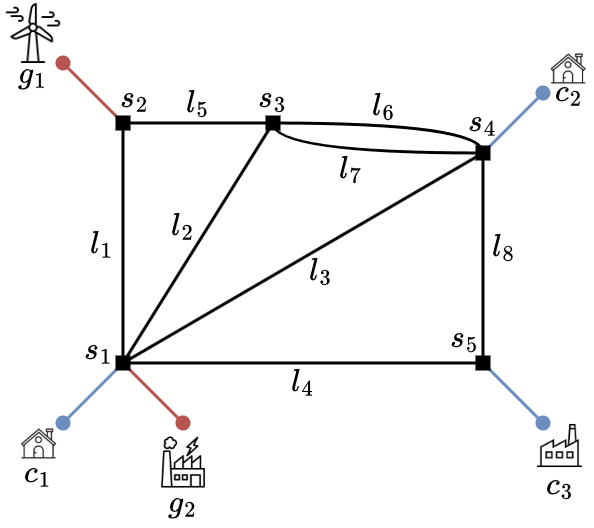
\includegraphics[width=0.45\textwidth]{images/background/simple_power_grid.png}
    \caption{Example of a simple power grid \cite{rl4network_operation}}
    \label{fig:simple_power_network}
\end{figure}

In electrical circuits a set of fundamental rules, called Kirchhoff's laws, define how the electricity flows through them:
\begin{quotation}
    \noindent
    \textbf{Voltage law:} Voltage around any closed loop sums to zero.\\
    \textbf{Current law:} Current entering and exiting any node sums to zero.
\end{quotation}
These laws also apply to power grids, which are essentially large, complex circuits \cite{rl4network_operation}. With the usage of the equations from Section \ref{ssec:electric-circuits} on delivered power, voltages and power loss, and Kirchhoff's laws, the behaviour of the power grid is analysed and predicted.

\subsubsection{Power Grid Components}
Each power grid has a variety of potential power sources. Traditionally, these sources were fuel-based (e.g. coal, natural gas and nuclear), located close to the cities that used them \cite{rl4network_operation}.
In modern power grids, power generation is also done using renewable energy sources, such as solar and wind power \cite{rl4network_operation}. These are often located in places far from any big cities, hence the distances to loads are greater \cite{RoleOfGridExtensionsEurope}. 
The distances between generators and loads are not the only difference with traditional power sources. Renewable energy sources also present a new challenge. 
These power sources are less predictable than traditional ones, as their generation of power relies on weather conditions and other factors \cite{challenges_integrating_var_renewables}. 
Consequently, they will not always produce electricity when it is needed. For example, if the highest power demand in winter occurs in the evening, solar panels are highly unreliable in countries such as those in the Nordic region, where the sun sets early in winter.
The different distances between generators and sources, and the variable power generation and demand, must be managed to maintain a stable power grid.

As already mentioned in Section \ref{ssec:electric-circuits}, for electrical systems there are two types of currents, \ac{ac} and \ac{dc}. When transporting electricity in the power grid with transmission lines, one of those two options has to be used. While \ac{dc} offers constant voltage transmission, \ac{ac} enables voltages to be raised or lowered using power transformers \cite{rl4network_operation}. Both allow high voltage transmission, though the variability of voltages in \ac{ac}, makes the transmission easier to control and less expensive than converters needed in \ac{dc} \cite{hvdcReviewIEEE}. For this reason power grids use mostly \ac{ac} \cite{rl4network_operation}. However, there are some use cases where \ac{dc} is used, such as \ac{hvdc}. In transmissions over far distances, like in submarine cables between countries or when transmitting power from offshore wind farms, \ac{hvdc} offers an advantage \cite{hvdcReviewEnergyWeek}. There is a transmission distance, where the total cost for \ac{dc} is lower than with \ac{ac}. This distance is called the break-even distance and is around 500 to 800km \cite{hvdcReviewIEEE}.
Furthermore, \ac{dc} transmission is used to connect two asynchronous \ac{ac} networks (networks with different frequencies). To make this possible a rectifier converts \ac{ac} to \ac{dc} and an inverter converts \ac{dc} back to \ac{ac} \cite{hvdcReviewEnergyWeek}.

The nodes connecting everything in the power grid are buses. Buses are single, fundamental electrical nodes, representing a single voltage level at a specific location, to which other grid components, like lines, loads or generators are connected \cite{pandapower}. Substations, on the other hand, contain multiple buses that together form a station-level-structure, which can be split or coupled. Splitting a substation means distributing grid components that are connected to the substation across multiple buses \cite{pptopogym}.

The power grid is split into four categories when it comes to the transport of power \cite{us_elec_industry_primer}. 
The \textbf{high voltage transmission grid} and \textbf{transmission grid} operate at high voltages for long-distance transport from large generation sites to regional substations. The high voltage transmission grid works above 765 kV \cite{us_elec_industry_primer}, while the transmission grid is maintained between 100 kV and 765 kV \cite{grl4powergrids}.
The \textbf{sub-transmission grid} is an intermediate layer which connects transmission substations to distribution substations and maintains voltages under 70 kV \cite{us_elec_industry_primer}.
The last layer is the \textbf{distribution grid}, which operates at the lowest voltages to safely deliver power to consumers. It manages voltages under 34 kV \cite{us_elec_industry_primer}. Most households receive power at much lower voltages. For example, households in Europe receive 230 volts and households in North America 120 volts \cite{rl4network_operation}. To ensure safe power delivery to homes, a step-down transformer is required to lower the voltage for local distribution \cite{rl4network_operation}.

Among these four categories, this thesis focuses specifically on the \textbf{transmission grid}, as this is the level at which \acp{tso} (see Section \ref{ssec:ctrl-power-grids}) actively manage power flow and grid stability.


% ++++++++++++++++++++++++++++++++++++++++++++++++++++++++++++
\subsection{Controlling Power Grids}\label{ssec:ctrl-power-grids}
As discussed in the previous sections, power grids contain multiple components. These have constraints, characteristics and behaviours to consider when operating on a power grid. This section presents the key aspects of power grid operation and explains how control centres, operated by \acp{tso}, manage the \textbf{transmission grid} to ensure stability and reliability.

\subsubsection{Constraints and Characteristics of Power Grids}\label{sssec:const_character_pg}
There are three primary constraints to ensure a stable power grid. Firstly, as previously mentioned, heat loss damages the network lines. For this reason the thermal limits of each line must be respected, and the voltage must be kept high to avoid exceeding them. Secondly, the voltage has to be in a correct range, as voltages must be kept high for transmission and lower for delivery to loads. 
Grid voltage must typically remain within $\pm10\%$ of its nominal rated value for low-voltage networks \cite{en50160}, though tighter limits may apply in transmission grids depending on national grid codes \cite{ansi_c84}. This ensures that the equipment operates safely and the power grid remains stable and reliable.
Lastly, generation and load must be balanced at all times. If power generation exceeds demand, then the power grid becomes unstable. Conversely, if there is not enough power to deliver to the loads, then power outages happen. 
Despite these constraints, operating the power grid is a time-domain challenge \cite{rl4network_operation}. Power grids have a brief window in which they can exceed their limits without the system collapsing. Solutions do not have to be implemented immediately when lines are overloaded. A short overload does not result in immediate disconnection, but the aim must always be to keep the grid in a stable state.

In addition to these constraints, the characteristics of power grids must be considered. Firstly, a power grid is a meshed network, meaning it contains many potential network states \cite{grl4powergrids}. The grid contains a number of switchable components, such as lines that are switched in or out of service, and busbars at substations that are split or coupled \cite{rl4network_operation}. These components enable electricity to be redirected and the flow to be controlled. Figure \ref{fig:power_op} illustrates this behaviour, showing the substation $s_3$ being split on two buses, to separate the flow coming from $s_1$ and $s_2$, while the line $l_3$ is out of service. 
Lastly, power grids are static in the sense that network operators cannot create new interconnected elements whenever they are needed. Expanding a power grid is a time-consuming process involving the construction of new grid elements \cite{rl4network_operation}.

\begin{figure}[htp]
    \centering
    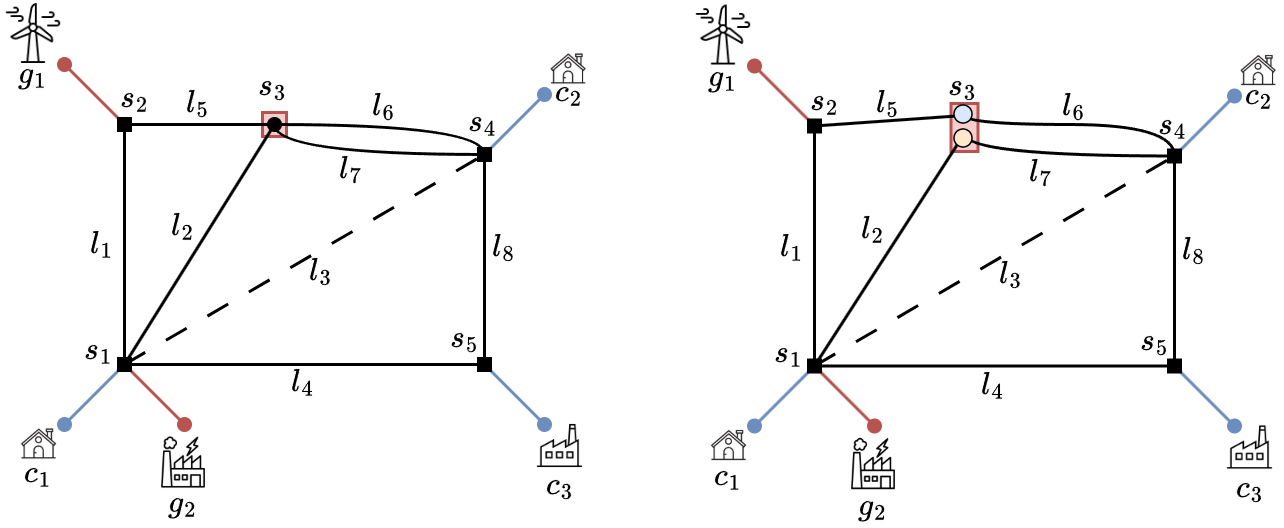
\includegraphics[width=0.9\textwidth]{images/background/power_grid_operation.png}
    \caption{Example of substation splitting and out of service lines (indicated by dotted lines) \cite{rl4network_operation}}
    \label{fig:power_op}
\end{figure}

\subsubsection{Operating on Power Grids}
The \ac{tso} chooses from a handful of actions, to operate on the power grid. The cheapest option is to switch lines in or out of service; splitting or coupling substations is more expensive. Increasing or reducing the output of a generator to adjust the flows on the lines is even worse in terms of costs, as it affects the energy market and increases costs for customers. Disconnecting loads is the most expensive action and should be avoided, as it causes disruptive effects on society, businesses, and people's daily lives \cite{rl4network_operation}. 

The transmission of power grids is controlled from control centres. These centres observe all elements of a grid and control some of them. 
For instance, they have full control over lines and substations via remote commands. Furthermore, they adjust the output of generators through remote instructions. Even some of the loads in a grid are controllable, though most of them are controlled by distribution system operators \cite{rl4network_operation}.

While a small to medium-sized country only has one control centre, larger countries (e.g. USA and Canada) have multiple control centres, which coordinate operations with neighbouring centres \cite{rl4network_operation}. 
These centres work continuously, as they must always comply with the constraints mentioned at the beginning of this section (thermal limits, voltage ranges, and the balance between generators and loads).
To increase the safety in a power grid, these centres must also be able to anticipate contingency states (i.e. states with unexpected failures or losses of key components). Examples of such techniques include $N-1$ or $N-k$ contingency analysis, in which the grid is simulated running with one or k elements removed \cite{nk_outages}. $N-0$ analysis is also used, which would be the base-case power flow simulation analysis, with no elements removed. These analyses enable operators to ensure safer operation even after failures occur.
Another possible situation is that there is a scheduled outage due to grid element maintenance.
Grid operators need to be aware of these situations and also plan for and manage system peaks during the day or during different seasons \cite{rl4network_operation}.



% ============================================================
% ============================================================
\section{Reinforcement Learning}\label{sec:rl}
\ac{rl} is a branch of \ac{ml} in which an agent interacts with an environment and learns to make decisions. Instead of learning from a fixed dataset, in \ac{rl} the agent receives feedback in the form of rewards, which it seeks to optimise. This design makes \ac{rl} particularly suited for solving decision-making problems, such as operating a power grid. This section provides the necessary background on \ac{rl}, by first explaining the fields of \ac{ml} in Section \ref{ssec:fields-learning} and then showing the theory and concrete algorithms of \ac{rl} in Section \ref{ssec:rl-terminology} and Section \ref{ssec:example-agents}. 

% ++++++++++++++++++++++++++++++++++++++++++++++++++++++++++++
\subsection{Fields of Learning}\label{ssec:fields-learning}
In the field of \ac{ml} there are multiple different types of learning. Each of them has different approaches to learning and how they are used varies significantly. While this thesis focusses on \ac{rl}, the fields of supervised and unsupervised learning are related to it.

\begin{figure}[htp]
    \centering
    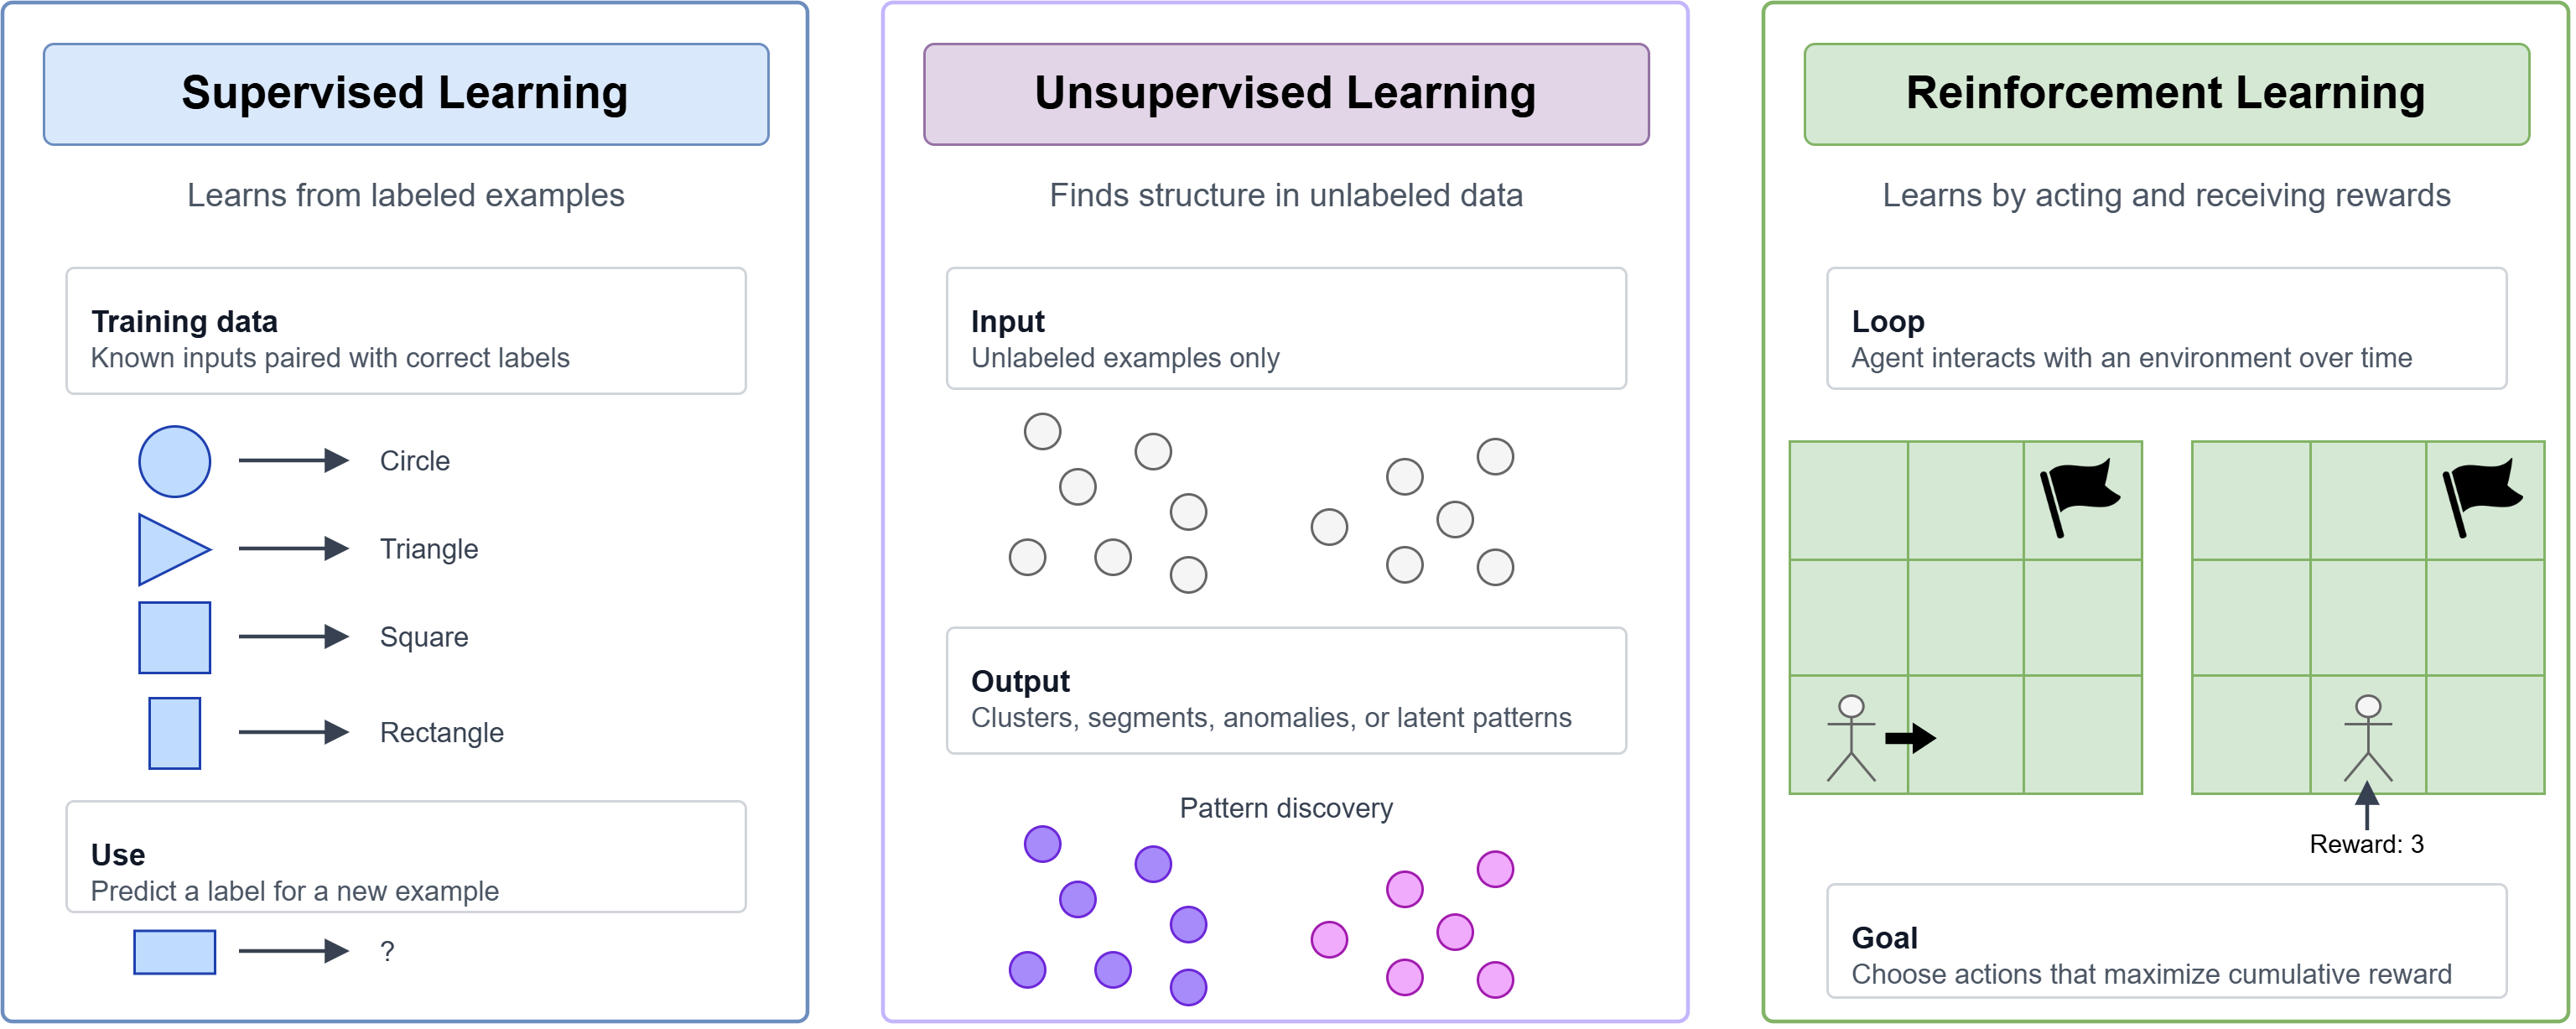
\includegraphics[width=0.96\textwidth]{images/background/learnings_example.png}
    \caption{Example of supervised, unsupervised and reinforcement learning}
    \label{fig:learnings_example}
\end{figure}

When the goal is to learn a function that maps inputs to correct outputs (labels), based on example input-output pairs, then supervised learning is useful. For the training phase in supervised learning a data set with correct labelling for each input is provided. This type of learning is supervised, as the data set is put together by some knowledgeable supervisor who will then observe how well the model predicts the labels \cite{rl_introduction}. 
Figure \ref{fig:learnings_example} demonstrates an example of supervised learning. The model receives a list of labelled data, a mapping of geometrical shapes and their names, and it uses this data to train. Once the model is trained, it labels new shapes using the knowledge it gained from the training data. Depending on the types of labels, supervised learning problems are categorised as either classification (when the label is a discrete category, as in the shape example) or regression (when the label is a continuous value) \cite{statisticalLearning}. Forecasting is a common application of regression. The model learns a mapping from time (and possibly other features) to a continuous predicted value (e.g. forecasting the weather for the next hours as seen in Section \ref{sec:application-power-grids}).

When the data is unlabelled and the goal is to find structure behind the data that might not be visible, then it is called unsupervised learning \cite{rl_introduction}. For example the unlabelled data seen in Figure \ref{fig:learnings_example}, where each data point is scattered around a two-dimensional plane. The model searches for a structure in this data, by choosing labels for each of the data points. In this case the cluster on the left and the cluster on the right are recognised and grouped, giving each point in each cluster a label (showcased as colour in the example), with each point in one cluster having the same label.

\ac{rl} takes a different approach in learning, as it is an optimisation problem seeking to improve a strategy $\pi$, called policy, to maximise reward. In Figure \ref{fig:learnings_example} the goal of the \ac{rl} agent is to move to the finish line. Every time the agent moves and lands in a new state a reward is returned. In this example the reward should be minimised, as the reward is the distance to the finish line. Hence, whenever the agent moves away from the finish line, a worse reward value will be returned, signalling to the agent, that it is moving away from the goal. As seen, \ac{rl} agents are interactive and goal-directed \cite{rl_introduction}, making decisions sequentially and learning with the reward to improve the actions selected by the agent. Supervised and unsupervised learning, however, have a fixed dataset and do not interact with any environment. The next section will explain in more detail how \ac{rl} is structured.


% ++++++++++++++++++++++++++++++++++++++++++++++++++++++++++++
\subsection{Reinforcement Learning Terminology}\label{ssec:rl-terminology}
This section summarises the key terminology of \ac{rl}, providing the formal framework and vocabulary necessary to understand the algorithms discussed later in this thesis. Based on the intuitive introduction to \ac{rl} given in Section \ref{ssec:fields-learning}, the following definitions formalise the concepts of states, actions, rewards and policies that form the basis of the interaction between an agent and its environment. The main source of the definitions of this section comes from \citet{rl_introduction}.

The environment of \ac{rl} is often modelled as a \ac{mdp}, which is a tuple that generally has the elements $\langle \mathcal{S}, \mathcal{A}, \mathcal{T}, \mathcal{R}, \gamma \rangle$. 
$\mathcal{S}$ represents the possible states of the environment, some states are also terminal (e.g. in cases of violation or exceeding a limit of the environment). A state contains the complete, exact description of the environment at a given time. In some cases, however, the agent does not have access to the full state, but only to an observation of it. This contains partial information about the state and models what the agent actually perceives of the environment \cite{openaiRLIntro}. Such settings are formally modelled as a \ac{pomdp} rather than a standard \ac{mdp} \cite{pomdp}. $\mathcal{A}$ represents the action space, while $\mathcal{T}$ describes the dynamics of the environment. Formally, $\mathcal{T}(s',r|s,a) = \Pr\{S_{t+1}=s', R_{t+1}=r \mid S_t=s, A_t=a\}$ is the joint probability of transitioning to state $s'$ and receiving reward $r$, given that the agent is in state $s$ and takes action $a$. From this, the state-transition probabilities are derived as $p(s'|s,a) = \sum_{r \in \mathcal{R}} \mathcal{T}(s',r|s,a)$, describing the probability of reaching state $s'$ given state $s$ and action $a$.
For a state $S_t \in \mathcal{S}$ in the timestep $t$, the agent selects one possible action $A_t \in \mathcal{A}$. This leads to the state $S_{t+1} \in \mathcal{S}$ and the reward $R_{t+1} \in \mathcal{R} \subset \mathbb{R}$, sampled according to $\mathcal{T}$. The reward is an immediate feedback to the agent on its decision.
Figure \ref{fig:rl-loop} shows these steps that are part of the whole \ac{rl} loop for each timestep $t$. For each step the agent receives the new state and reward and decides the next action. 
The factor $0 \le \gamma \le 1$, also called discount factor, balances the importance of future rewards against immediate ones. This is used for the discounted return 
\[G_t = R_{t+1} + \gamma R_{t+2} + \gamma^2 R_{t+3} + \cdots = \sum_{k=0}^{\infty} \gamma^k R_{t+k+1}\] 
where $\gamma^{k}$ defines how much weight a reward received $k$ timesteps in the future has. In a finite \ac{mdp} there is the horizon $H$, which defines the length of an episode, where the timesteps are defined as $0 \le t \le H$. 

\begin{figure}[htp]
    \centering
    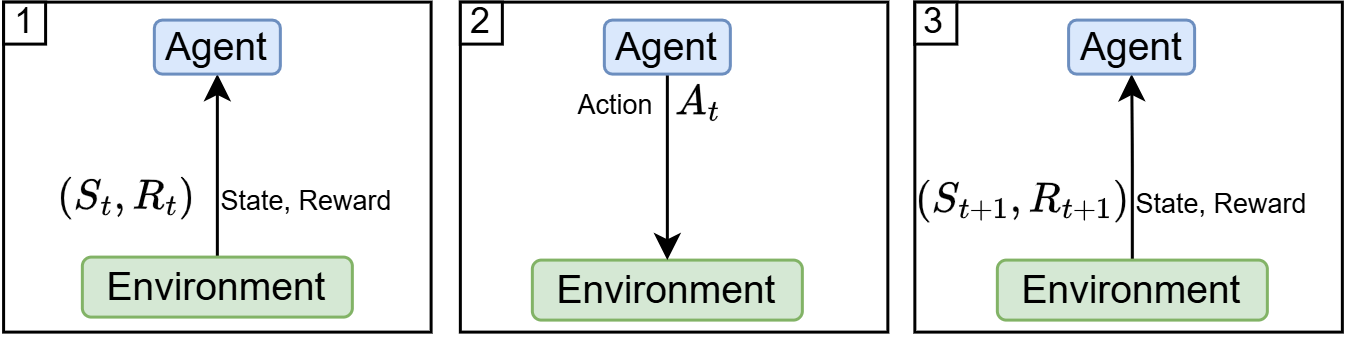
\includegraphics[width=0.8\textwidth]{images/background/RL_loop.png}
    \caption{Steps of the \ac{rl} loop at timestep $t$}
    \label{fig:rl-loop}
\end{figure}

The agent's \textbf{policy} $\pi:\mathcal{S} \times \mathcal{A} \rightarrow [0,1]$ represents the decision-making strategy that the agent follows. Simply said the policy is a mapping that decides for each state, with what probability it chooses an action. If the policy is deterministic and not stochastic, it creates a direct mapping from state to action to take \cite{openaiRLIntro}. While the reward is an immediate feedback, on the long run the \textbf{value function} $v_{\pi}(s)$ defines how favourable a state is for the agent. It defines for the agent how favourable the current state $s$ is under policy $\pi$ for future timesteps, expressed as the expected cumulative reward. The formal definition is
\[v_{\pi}(s) = \mathbb{E}_{\pi}\!\left[ G_t \mid S_t = s \right]\]
with $\mathbb{E}_{\pi}\!\left[ \cdot \right]$ being the expected value given that the agent follows policy $\pi$. 
The expected return is defined as the value of taking action $a$ in state $s$ under the policy $\pi$ and is denoted as 
\[q_{\pi}(s,a) = \mathbb{E}_{\pi}\!\left[ G_t \mid S_t = s, A_t = a \right]\]
In value-based algorithms the goal is to learn and maximise expected value and return \cite{rl2grid}. In case of finite \ac{mdp}, the agent's goal is to maximise the expected cumulative discounted sum of rewards over these timesteps \cite{grl4powergrids}.

For learning the agent's strategy, there are two approaches in \ac{rl}. For \textbf{on-policy} algorithms, they learn and update their policy through actions taken by their own policy. In each step the policy decides the next action and with the resulting data, the same policy is updated. 
\textbf{Off-policy}, on the other hand, uses two policies. The target policy is the policy that is being learned and improved, while the behaviour policy controls the agent's actions and generates the data that is used to update the target policy. As the target policy differs from the behaviour policy that generates the data, off-policy algorithms learn from data collected by any policy. This includes past versions of the behaviour policy. This is unlike on-policy algorithms, which require data generated by the exact policy being updated.

For the next immediate timesteps, \ac{rl} systems may also utilize a model of the environment, which simulates its behaviour and enables predictions of how it responds. It can be used to predict the reward, depending on a state and action that was chosen. \ac{rl} systems that use these models are called \textbf{model-based} and those without are known as \textbf{model-free}. Model-based learners plan ahead, while model-free systems are trial-and-error learners. 

Another parameter that needs to be chosen in a \ac{rl} algorithm is whether the agent favours \textbf{exploration} or \textbf{exploitation}. When the agent favours exploration, it aims to visit new states to discover more about the environment. As for exploitation, the agent uses the current knowledge to maximise reward in each step. Exploration provides insights into the environment, expanding the knowledge that the agent collects about it. Exploitation uses this knowledge to improve the agent's strategy. This illustrates the exploration-exploitation dilemma. Relying solely on exploration prevents the agent from exploiting its accumulated knowledge, while relying solely on exploitation prevents it from discovering potentially better actions. Thus it is important to find a suitable balance between these two approaches, in order that the agent continues to learn and improve itself.

% ++++++++++++++++++++++++++++++++++++++++++++++++++++++++++++
\subsection{Example Agents}\label{ssec:example-agents}
One simple example of an agent is a \textbf{greedy} agent. The following equation defines its strategy. 
\[A_t \doteq \underset{a}{\arg\max}\, q_t(s_t, a)\]
Here, $A_t$ is the action selected at timestep $t$, and $q_t(s_t, a)$ is the agent's current estimate of the value of taking action $a$ in state $s_t$. The greedy agent always aims to choose the action with the highest estimated value. 
It has no explorative strategy at all, which makes the reward estimation harder and less precise. When the rewards are noisy, more exploration is necessary to find an optimal action. An explorative alternative to the greedy agent is the \textbf{$\varepsilon$-greedy} algorithm, which adds randomness to the greedy agent's actions. With a probability of $\varepsilon$, the agent performs a random action, in order to explore the environment more. The higher this probability, the more explorative and less exploitative the agent becomes \cite{rl_introduction}, illustrating the exploration-exploitation dilemma introduced in Section \ref{ssec:rl-terminology}.

\subsubsection{Value-based agents}
A classical value-based algorithm is \textbf{Q-Learning}. It aims to improve the policy by updating values in a Q-table using an off-policy approach. This is a lookup table where each entry $q(s,a)$ is a heuristic for how favourable it is to take action $a$ in state $s$. The goal is to create a heuristic for the optimal action-value function
\[q^*(s,a) = \mathbb{E}_{\pi}\!\left[ R_{t+1} + \gamma\ \max_a\ q(S_{t+1}, a) \mid S_t = s, A_t = a \right]\]
which is the Bellman optimality equation in an action-value form \cite{foundationsRL}. This is achieved by improving the lookup table iteratively. The needed information for this is $(s_t,a_t,r_{t+1},s_{t+1})$, where $a_t$ is derived from the behaviour policy and a system model generates $r_{t+1}$ and $s_{t+1}$. The update of the Q-table is done with the following function 
\[
q_{t+1}(s_t,a_t) \leftarrow q_t(s_t,a_t) - \alpha_t(s_t,a_t)
\Big[q_t(s_t,a_t) - (r_{t+1} + \gamma \max_a q_t(s_t,a))\Big]
\]
with $q_t(s_t,a_t)$ being the current estimation on how favourable action $a_t$ is in state $s_t$ is, $\max_a q_t(s_t,a)$ as the best estimated value of the next state and $\alpha_t(s_t,a_t)$ being the learning rate, controlling the update magnitude \cite{foundationsRL}. In summary, the update can be summarised as
\[
\text{new estimate} = \text{old estimate} + \text{step size} \times \text{error}
\]
thus, the current estimate is moved towards a better estimate using the current error. The target policy is then updated with 
\[
\pi_{t+1}(a \mid s_t) =
\begin{cases}
1 & \text{if } a = \arg\max_a q_{t+1}(s_t, a), \\
0 & \text{otherwise}
\end{cases}
\quad \text{\cite{foundationsRL}.}
\]

A variation of this is \textbf{\ac{dqn}}, which uses a deep neural network to approximate the Q-values \cite{grl4powergrids}. In general, \ac{rl} algorithms that use a deep neural network to represent their policy, value function or model of the environment are called \ac{drl} algorithms. They combine deep learning with \ac{rl} \cite{deepRLIntro}.

\subsubsection{Policy-based}
A pure policy-based algorithm is \textbf{Monte Carlo Policy Gradient (REINFORCE)}. It uses a parameterised stochastic policy $\pi_\theta$ and its goal is to maximise $J(\theta)$, which is the expected return under $\pi_\theta$. For each episode of the algorithm, a trajectory $\{s_0,a_0,r_1,...,s_T\}$ is generated using the current policy $\pi_\theta$. Then the policy is improved by iterating over all $t=0,...,T-1$. This is done by first updating the value with 
\[
    q_t(s_t, a_t) = \sum_{k=t+1}^{T} \gamma^{\,k-t-1} r_k
\]
which is the return from time $t$. This is used for the Monte Carlo estimation $q_\pi(s_t,a_t) \approx q_t(s_t, a_t)$ of the action-value function under policy $\pi$ \cite{foundationsRL}. To update the policy the function
\[
\theta \leftarrow \theta + \alpha \, \nabla_\theta \ln \pi_\theta(a_t \mid s_t)\, q_t(s_t, a_t)
\]
is used \cite{foundationsRL}. $\alpha$ is the learning rate, which defines the size of the update steps, and $\nabla_\theta$ is the gradient operator. When the return from time $t$ $q_t(s_t, a_t)$ is high, the probability of $a_t$ is increased, when it is low it will be decreased. The gradient $\nabla_\theta \ln \pi_\theta(a_t \mid s_t)$ is a vector, which gives a direction. Moving to that direction increases the probability of choosing $a_t$ in state $s_t$ \cite{rl_introduction}.

\textbf{Actor-Critic} is a policy- and value-based hybrid. The algorithm contains an actor, which learns policies to maximise rewards, and a critic, which evaluates the policies from the actor, by estimating the value function. This balances pure policy methods and pure value function methods. While the critic stabilises learning, the actor handles action selection. Variations of this are the \textbf{\ac{a3c}} and \textbf{\ac{ppo}} algorithms. In \ac{a3c} multiple agents run in parallel. While each agent collects experience independently a shared global model is updated asynchronously. In the case of \ac{ppo}, the policy updates are clipped in order to stabilise the training process by preventing large jumps in the policy, which could otherwise lead to oscillations \cite{grl4powergrids}.



% ============================================================
% ============================================================
\section{Benchmarks}\label{sec:benchmarks}
This section defines benchmarks and the principles to follow when creating them. 
Benchmarks are extremely important in development and research because they provide a shared reference point that clearly defines how improvement is measured. This standardised evaluation makes results interpretable and comparable across projects and teams \cite{mlperf_benchmark,ml_benchmarks}.
This drives progress when benchmarks and their results are published. It leads to competition between multiple developers and, furthermore, helps with improvement in research \cite{mlperf_benchmark, ml_benchmarks, building_benchmarks4models}.
Benchmarks are also used to compare specific aspects. For example, a benchmark that evaluates machine learning models could be used to compare different models, training configurations, or hardware systems \cite{ml_benchmark_design}.
This comparability also supports decision-making by indicating which evaluated inputs to use in the real world \cite{building_benchmarks4models}. 
Furthermore, benchmarks make it easy for inexperienced people to understand what constitutes strong or weak performance in the evaluated field \cite{building_benchmarks4models}. 

Section \ref{sec:rw-benchmarking} provides some examples of implemented benchmarks. It shows how the benchmarks are structured for different reinforcement learning and power grid scenarios.


% ++++++++++++++++++++++++++++++++++++++++++++++++++++++++++++
\subsection{Structure of a Benchmark}\label{ssec:structure-benchmark}
Figure \ref{fig:general-benchmark} shows a general structure that every benchmark shares. In simplified terms, a benchmark is an algorithm that reads an input and returns a rating of the input using one or more scores. Benchmarks come in many forms, as they are used in a variety of different fields, in and outside of science. Even in the same field benchmarks have many forms. While a \textbf{micro-benchmark} evaluates a specific component of a benchmarked entity, a \textbf{macro-benchmark} analyses a specific task and how well this entity performs in it. An \textbf{end-to-end benchmark}, on the other hand, evaluates how an entity performs in total, from start to finish \cite{ml_benchmark_design}.

As Figure \ref{fig:general-benchmark} demonstrates, a benchmark algorithm consists of multiple components. Firstly, in order to evaluate the input, the benchmark requires data or configurations that form part of its context. The data needed in a macro- or micro-benchmark covers much less of the input's context than an end-to-end benchmark, as the latter covers a much broader scope. In the macro- and micro-benchmark the data is specialised in one aspect of the input's context. Specified tasks are then performed on these data or with these configurations, to test the behaviour of the input in different situations. For each task, metrics are measured, which are evaluated by a scoring function. This function may use a baseline or reference values to convert the measured metrics into a specific score. Finally, the output is created by using the calculated scores or by aggregating them (e.g. by computing the average value).

\begin{figure}[htp]
    \centering
    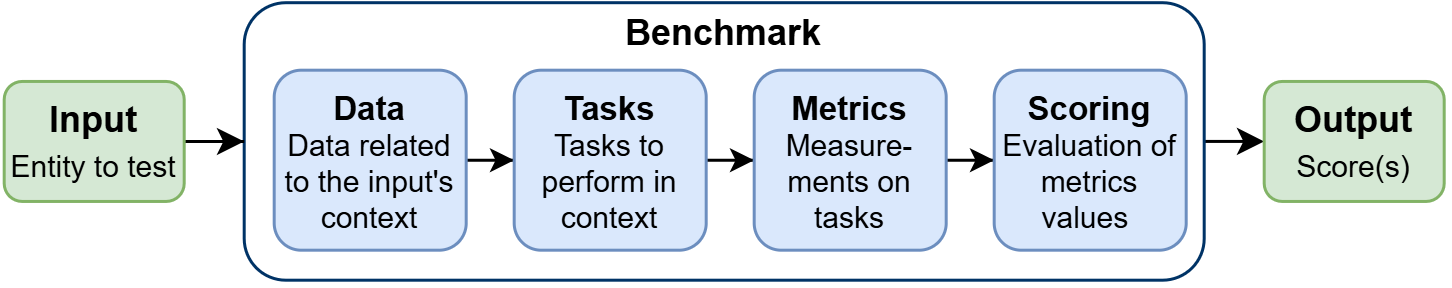
\includegraphics[width=0.8\textwidth]{images/background/general_benchmark_overview.png} 
    \caption{General structure of a benchmark}
    \label{fig:general-benchmark}
\end{figure}

% ++++++++++++++++++++++++++++++++++++++++++++++++++++++++++++
\subsection{Principles of a Benchmark}\label{ssec:principles-benchmark}
In order to construct a benchmark, there exists a series of principles that must be followed. In their absence, the relevance of a benchmark might be questionable, and its capacity to drive progress in the field might be limited. This section will provide a comprehensive overview of the fundamental principles that must be observed when constructing a benchmark, to ensure its quality. 

\paragraph{Definition of the Objective.} 
It is essential to define the objectives of the benchmark prior to its development. It must be clear what kind of goals or improvements the benchmark wants to achieve (e.g. cost-efficiency, quality of input-entity, speed or computational efficiency, etc.). By establishing these criteria at the initiation of the process, it is clear which data, tasks and metrics to use and which ones are not relevant. With this, the benchmark is precise with the resources it is using, not omitting anything important and not using any unneeded resources. 

\paragraph{Reproducibility.}
The utilisation of a benchmark must ensure reproducibility, thereby guaranteeing that the same input always yields the same output score. This is of fundamental importance for the reliability and comparability with other inputs. Certain benchmarks select context and tasks at random for a given input. This approach is appealing as it allows for the testing of diverse scenarios in each iteration, though it complicates the comparison of different inputs. In this particular instance, it is necessary for the benchmark to include a configurable seed, thus enabling the testing of two distinct inputs using the same seed and, by consequence, the same scenarios. Furthermore, reproducibility is ensured by creating a standardised evaluation algorithm. The data, tasks, metrics and scoring inside the benchmark must always follow a fixed and predefined structure.

\paragraph{Comparability.}
The ability to make meaningful comparisons is a crucial aspect of establishing a high-quality benchmark. Without the implementation of effective comparability measures, it is challenging for users to identify the most effective input or to determine whether they were enhancing the benchmarked inputs. Comparability does not necessarily imply that it is obvious which input was the best. Two different inputs may have their own strengths and weaknesses and perform better in certain scenarios than others. 

\paragraph{Transparency.}
If the benchmark is built transparently, so that the user understands how the output scoring is being calculated, it becomes more comprehensible, what the strengths and weaknesses of each input are. Perhaps one input is suitable for a specific task, or perhaps it performs perfectly in general but has some weaknesses. To achieve transparency, the outcomes of the benchmark must be interpretable, so that users can understand what the scores mean, how they are calculated, and how they relate to the performance of the input. With sufficient transparency and reproducibility, users can get a clear idea of how their inputs perform, which one to use in which situation, and which aspects to improve.

\paragraph{Relevance.}
A benchmark must be relevant to the field in which it is used. The evaluation data has to be reliable, representing the context in which the inputs are tested and aligning with real-world scenarios in which the inputs are used. Otherwise, the inputs will not encounter the problems and challenges present in real applications. 

\paragraph{Representativeness.}
Furthermore, the benchmark must be representative, meaning diverse scenarios and edge cases have to be covered to ensure the inputs are suitable for all use cases. Of course, this depends on what the benchmark tests. If it is a very specific test (e.g. a macro-benchmark, as described in \cite{ml_benchmark_design}), then the scenarios may be very similar, as the evaluation focuses on one aspect. However, if the benchmark tests generalisation and how well the inputs behave in different scenarios, it must be free from bias and ensure a fair comparison between different approaches.
    \chapter{Related Work}\label{ch:related-work}
This chapter provides a comprehensive overview of the preceding works that are related to the subject of this thesis. This chapter first presents the use cases of different \ac{ml} algorithms in the field of power grids and its operation. Secondly, a series of past works will be presented, providing both general and power grid-specific benchmarks for \ac{rl} algorithms.


% ============================================================
% ============================================================
\section{Applications on Power Grids}\label{sec:application-power-grids}
This section is focused on past work on the application of \ac{ml} algorithms on power grids. Firstly, a number of examples will be given of forecasting systems, which provide estimates of future states of grid components. Subsequently, an analysis of a range of \ac{rl} algorithms that control power grids with different objectives will be made. The following summary will demonstrate how past works have already demonstrated the usefulness of \ac{rl} agent-based control systems in managing grids, and how they are used in a variety of situations, from the control of specific grid components to the alteration of the grid's topology in order to optimise power flow. 


% ++++++++++++++++++++++++++++++++++++++++++++++++++++++++++++
\subsection{Forecasting Systems}
Supervised learning approaches are useful for forecasting systems in power grids. Most of these systems solve a time-series problem, meaning the data is time-dependent. These systems are trained to predict specific labels in the grid at future timestamps, which helps maintain grid stability. 
Studies such as \citet{shortTermLoadForecasting} and \citet{loadForecastingDeepNN} demonstrate how short-term load forecasting is achieved using supervised learning. This is useful for cost estimation for power grid customers, or for predicting energy needs in order to plan when to generate more or less power.

Regarding generators, works such as \citet{meka2021robust} demonstrate how a model that forecasts wind generation is trained using meteorological data together with wind power production. This helps manage the variability caused by wind generation, as with other renewable energies, and makes it easier to integrate wind energy into power grids. 

Regarding the entire power grid, the work of \citet{ngo2024physics} focuses on the implementation of a GNN, which estimates the state of power grid components. This paper presents a common representation of power grids as graphs, where the nodes represent buses and the edges represent transmission lines. This representation is evident in other frameworks and simulation environments, which will be discussed in later sections. Supervised learning is used to train and estimate bus voltage magnitudes, voltage phase angles, and other power grid states using grid measurements.


% ++++++++++++++++++++++++++++++++++++++++++++++++++++++++++++ 
\subsection{Grid Control Systems}\label{ssec:grid-ctrl-systems}
\ac{rl} has use cases in grid control, since power grid operation involves decision-making that needs to be optimised. The \ac{rl} agent performs sequential control decisions while improving its policy to achieve a more stable grid and optimal resource usage. 
Using \ac{rl} for this problem has become more important as the proportion of renewable energy in power grids has increased, as previously mentioned, and these sources have a more unpredictable power generation pattern. Improvements in \ac{rl} and \ac{drl} now enable agents to solve complex problems involving large data sets \cite{glavic2017reinforcement}. Due to this progress, more researchers have attempted to use \ac{rl} for power grid operation \cite{fan2022powergym}.

The typical actions in power grid operation can be divided into three categories. \textbf{Control actions} manage the adjustable components of the power grid. For example, dispatch actions control power generation by increasing or decreasing the output of power plants to match the current load demand. Another example is voltage control throughout the grid. \textbf{Topology actions} modify the grid's configuration, e.g. by opening or closing transmission lines, changing the busbar to which a line is connected, or splitting or merging substations. These actions are useful for controlling power flow in the grid and for avoiding or handling congestion (overloaded transmission lines). The final type of action is \textbf{protection} or \textbf{emergency action}. These actions prevent cascading failures and attempt to restore the grid to a safe state. Examples include load shedding, which disconnects part of the loads from the power grid to temporarily reduce the power demand for the grid, generator tripping, which disconnects generators from the grid to protect them \cite{protecting_synchronous_generators}, or emergency switching, which changes the network's topology to prevent cascading failures throughout the grid components.

\subsubsection{Control Actions on Power Grids}
The work of \citet{glavic2017reinforcement} shows how \ac{rl} has already been used in past research for grid control or emergency actions. Figure \ref{fig:rl-framework-powergrid} shows a framework for building a \ac{rl} algorithm that makes decisions over a power grid, as mentioned in the work. The research mentioned in this paper has considered \ac{rl} agents for a variety of use cases, such as making market decisions through electricity market simulations and controlling the grid, including voltage control, automatic generation control, power demand control, and system restoration to bring the power grid back to a stable state. This work demonstrates how \ac{rl} is already considered an effective approach to solving a variety of control and decision problems in power grids.

\begin{figure}[htp] 
    \centering
    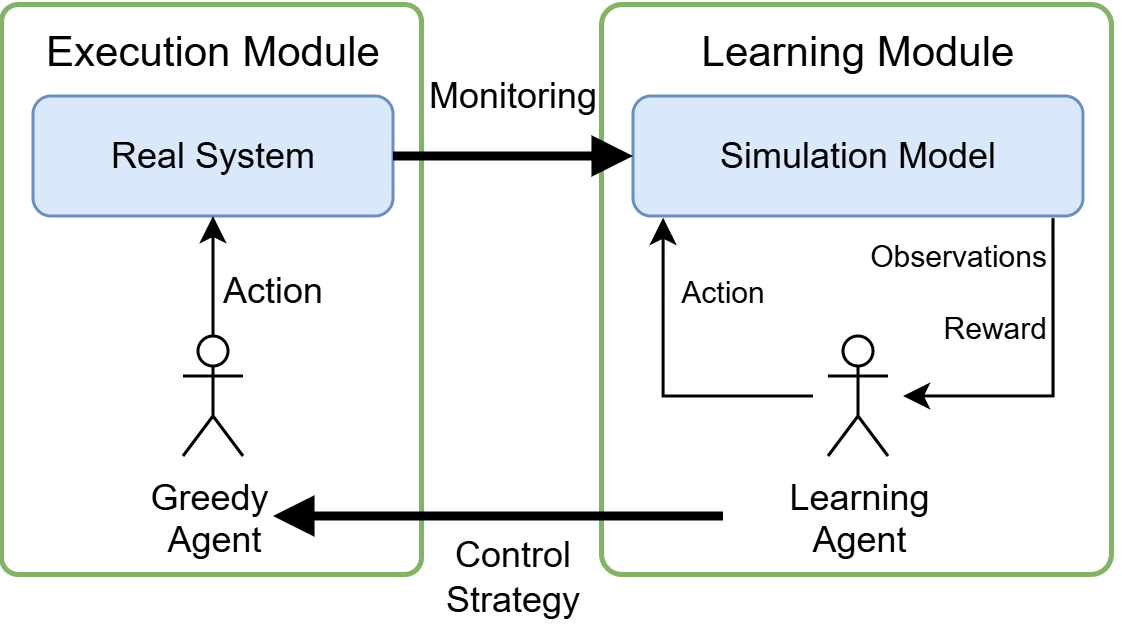
\includegraphics[width=0.8\textwidth]{images/related_work/RL_framework_glavic.png}
    \caption{Framework for a \ac{rl} algorithm in power grid decision and control}
    \label{fig:rl-framework-powergrid}
\end{figure}

Another grid control approach is presented in \citet{barg2023deep}, which uses \ac{drl} to regulate voltage levels at all buses to ensure reliable operation. Each state in the \ac{rl} algorithm contains information on the bus voltages, power flows and network conditions. The agent's actions use controllable grid components to regulate voltage levels. The agent is rewarded for keeping voltages within limits, reducing voltage violations and avoiding unnecessary control actions \cite{barg2023deep}.


\subsubsection{Topology Actions on Power Grids}
A considerable amount of research has been conducted on topology actions involving \ac{rl}. One important research project in this area is the \ac{l2rpn} challenge. The aim of this challenge is to design agents that operate safely over power grids. 
To run the agents for the challenge, the \textbf{Grid2Op} framework was developed. This section refers to the paper by \citet{l2rpn} for details of \ac{l2rpn} and to the Grid2Op documentation to summarise Grid2Op.

Grid2Op emulates the behaviour of a power grid, exposing agents to maintenance operations and topology changes within the grid. The framework focuses on \ac{rl} development and enables actions such as connecting or disconnecting transmission lines, moving grid components (e.g. lines, generators, and loads) to another busbar, redispatching generators, curtailing renewable generators (i.e. asking them to produce less than they are capable of), and controlling power storage units. Grid simulations commonly use \textbf{pandapower}, an open-source library for power system modelling and analysis. This tool enables the simulation of \ac{ac} and \ac{dc} power flow, the execution of \ac{opf}, and the analysis of network states over time \cite{pandapower}.

The paper by \citet{l2rpn} presents the results of the \ac{l2rpn} challenge. For this, an industry-standard synthetic network was used, and the agents had to comply with a few constraints. Deterministic events, such as maintenance, and stochastic events, such as targeted attacks by an adversarial opponent, can disconnect power lines for several hours. Additionally, if a line is overloaded for too long, it automatically disconnects, which can lead to cascading failures. The agent must wait before using these lines again, as it takes a few hours for them to be reconnected. Furthermore, to prevent the overuse or failure of expensive network components, the agent is not permitted to act on the same component too frequently. The agent's run is terminated by a "Game Over" condition when the total demand is not met. In the \ac{l2rpn} challenge, only two actions are permitted: topology changes and changes to the power generation of the power plants within the grid. Each action is checked against the previously mentioned constraints before being fed into a power flow simulator to calculate the next network state.

Each of the participants' agents went through 24 test scenarios. For each scenario, the participants were given a validation dataset during training and a test dataset for the final leaderboard. The evaluation and scoring of each agent are discussed in detail in Section \ref{ssec:power-benchmark}. 
Of the approaches, the three best ones all used \ac{rl} to solve this optimisation problem. 
The agent with the best performance reduced the possible actions to 1000 to reduce complexity. They used a policy parameterised by a neural network with a few million parameters, which they trained with an evolutionary algorithm instead of standard \ac{drl} strategies (e.g. \ac{ppo} or \ac{dqn}). In the evolutionary algorithm, multiple policies were trained and the best ones were selected and mutated, iteratively improving the policy weights. 
The second-best agent initially used expert-guided exploration to reduce the action space to 200 actions. They then trained a neural network to imitate this expert agent, although this imitation agent performed slightly worse. Finally, they used an actor-critic model with \ac{ppo}, initialised with the imitation agent and trained to improve long-term planning. This improved their strategy, earning them second place in the challenge. The third-best-performing agent used a \ac{dqn} variation that directly learns a policy mapping grid states to topology actions.

This challenge encouraged many participants to develop different approaches to solving the problem of power grid operation. The Grid2Op framework made it possible for many developers and researchers to begin researching agents in the power grid domain. The resulting agents demonstrated robustness in challenging grid scenarios, successfully handling long action sequences even under strong perturbations. Notably, agents showed the potential to augment knowledge of grid flexibility beyond human capability, which would already be valuable for grid operators. This suggests that \ac{ml} algorithms, particularly \ac{rl}-based approaches, hold promise as tools to support \acp{tso} in grid operation.

Similar to Grid2Op, the work by \citet{pptopogym} presents \textbf{PPTopoGym}, a lightweight topology optimisation environment that uses the pandapower library for data structures and power flow calculations. Furthermore, it offers the computation of $N-1$ power flow to test how stable the power grid remains if one line is removed. This feature is not included in the \ac{l2rpn} competitions, as mentioned in Section \ref{ssec:power-benchmark}. The PPTopoGym environment supports topology actions such as substation reconfiguration, as well as line, switch and transformer switching \cite{pptopogym}.

Another survey discussing topology actions in power grids is done by \citet{grl4powergrids}. It focuses on \ac{gnn} and how to use them in \ac{grl}. Since power grids can be naturally modelled as graphs, \acp{gnn} combined with \ac{rl} are suitable for this optimisation problem. \acp{gnn} have the functionalities required for feature extraction in graph-structured data, helping \ac{rl} agents to understand complex relationships within grids and make better decisions. The survey presents approaches to \ac{grl} used in topology actions across power grids. In these approaches, the grid state is modelled as a graph from which a \ac{gnn} extracts features. Grid states contain grid topology information, such as bus, generation and load connections, as well as voltages and power flows in transmission lines. The agent's rewards are calculated based on these power flows, the extent to which grid congestion is mitigated, and the level of operational cost reduction.



% ============================================================
% ============================================================
\section{Benchmarking}\label{sec:rw-benchmarking}
This section presents previous benchmarking studies in the field of \ac{rl}. It summarises the structure of different benchmarks, using the principles outlined in Section \ref{ssec:principles-benchmark} to evaluate each benchmark's design.


% ++++++++++++++++++++++++++++++++++++++++++++++++++++++++++++
\subsection{Reinforcement Learning Benchmarking}
An established standard for training and testing \ac{rl} agents is \textbf{OpenAI Gym} \cite{gymnasium}. The paper by \citet{gymnasium} showcases the features of this toolkit, which standardises the development and evaluation of \ac{rl} algorithms. OpenAI Gym provides a variety of environments, including control problems, Atari games, and robotics environments. Each agent is evaluated based on its episodic cumulative reward (return) achieved in the test environments, and there used to be a website with a scoreboard where researchers and developers could reproduce or compare other approaches by examining their source code. After OpenAI Gym was no longer maintained, \textbf{Gymnasium} became its successor. The paper by \citet{gymnasium} demonstrates how Gymnasium, just like OpenAI Gym, has become a popular toolkit with millions of downloads since its release. Like OpenAI Gym, Gymnasium contains a standardised environment interface and has built-in environments. Additionally, it has a large ecosystem of external environments, and it is possible to use it with various training libraries (e.g. Stable Baselines 3, CleanRL and Ray RLlib). Like OpenAI Gym, Gymnasium does not benchmark agents directly, but instead offers standardised environments for testing agents. According to the benchmark structure defined in Section \ref{ssec:structure-benchmark}, it contains the data and tasks required for a benchmark evaluation. However, it lacks the metrics and scoring system necessary to provide measurable feedback to agents.

A similar benchmark is the \textbf{Procgen} Benchmark mentioned in \citet{procgen}. Furthermore, it offers a variety of game-like environments. For each environment, a unique scenario is created using procedural generation. This benchmark measures sample efficiency, i.e. how effectively an agent learns from a limited number of experiences or interactions with its environment. Additionally, it measures generalisation, which is an agent's ability to perform well on new, unseen tasks. The procedural generation used in this benchmark is useful to control whether an agent has problems with overfitting to one specific scenario. This makes the benchmark representative by covering diverse scenarios and benchmarking edge cases procedurally. A final single score is calculated based on a mean normalised return value. As it only focuses on two tasks of an \ac{rl} agent, sample efficiency and generalisation, this benchmark is a macro-benchmark. However, when compared to other agents, this benchmark lacks information, as an aggregated score does not show the strengths and weaknesses of the agents, only their overall performance.


% ++++++++++++++++++++++++++++++++++++++++++++++++++++++++++++
\subsection{Benchmarking on Power Grids}\label{ssec:power-benchmark}
There is already past work on benchmarking \ac{rl} agents in power grids, some of which is strongly related to this work. Many of these existing tools use the IEEE test cases presented in \citet{matpower}. These are standardised power grid models offering different grids. For example, IEEE 30-bus, also known as case 30, consists of 30 buses, five generators and 41 lines \cite{matpower}. These models provide realistic grids of various sizes and levels of complexity, making them well-suited to accurately representing real-world scenarios in benchmarks. This section presents the benchmarks that utilise these test cases, and their design will be analysed. 

\subsubsection{PowerGym}
The \textbf{PowerGym} project, introduced in \citet{fan2022powergym}, benchmarks Volt-Var control systems in distribution grids. This means that agents must control voltage (Volt) and reactive power (Var) in order to minimise power losses and voltage violations within the grid. The components used to achieve this are voltage regulators, switchable capacitors, and controllable batteries. The capacitors regulate reactive power, while the batteries regulate active power.
An OpenAI Gym interface is used for the benchmark, making it easier to use with existing \ac{rl} algorithms. The \textbf{OpenDSS} simulator is used for the physical power flow and the test environments are based on IEEE benchmark systems. The benchmarking system is designed solely to compare multiple approaches with each other in the same standardised Volt-Var control environment, where performance is measured using cumulative reward. This reward system penalises voltage violations, power losses, and frequent changes that wear out control devices. It is possible to modify the test environments to increase difficulty, e.g. by scaling the loads, which results in higher power consumption and makes grid stability more difficult.

As for the benchmark design, this work aligns with most of the principles. The objective is clear, as the Volt-Var control target task is specified throughout. Furthermore, it offers a standardised evaluation setup with fixed systems and a uniform structure, which provides reproducible results. As it is possible to evaluate different agents in the same environments, with the same system definitions and reward functions, PowerGym enables direct comparison of agents. Additionally, the paper provides a clear explanation of how the benchmark works and what it evaluates. Lastly, the benchmark is relevant to the application domain as it uses OpenDSS and diverse IEEE test scenarios for simulation, providing sufficient coverage of Volt-Var control scenarios. However, some principles are lacking, such as the fact that the benchmark only provides one cumulative reward score, which might hide the strengths and weaknesses of an agent. Moreover, the environments used in the benchmark only cover four systems, which may not represent every edge case or common scenario. A more diverse selection of scenarios allows for a more in-depth evaluation of agents.

\subsubsection{L2RPN}\label{sssec:l2rpn}
As mentioned in Section \ref{ssec:grid-ctrl-systems}, \ac{l2rpn} is a competition-style benchmark built using the Grid2Op simulation framework. Benchmarking is performed through the \ac{l2rpn} challenge, in which each participant must complete 24 test scenarios. For each scenario, participants were provided with a validation dataset during training and a test dataset for the final leaderboard, with submitted code executed by an evaluation server. Each scenario received a normalised score ranging from -100 to 100, based on the cumulative network operational cost. A score of -100 was given if an immediate blackout occurred, and a score over 0 required the agent to perform better than a do-nothing agent (i.e. an agent that does not interact with the environment). If the scenario was completed without terminating early with a "Game Over", the agent received a score of 80. To achieve the maximum score of 100, the agent's operational cost must be 20\% lower than that of a baseline agent. The leaderboard was created by taking the sum of all the scores from the 24 scenarios.

As for the benchmark principles, this challenge followed most of them. \ac{l2rpn} had a clear objective in ranking the agents by having two sub-objectives, robustness and adaptability. For the adaptability, the agent's ability to handle unseen data distribution of renewable energy mixes is tested. Additionally, due to the fixed evaluation structure of the challenge, reproducibility was ensured, with a standardised evaluation server testing the submitted agents. As all the agents underwent the same process and a fixed set of scenarios and evaluation systems, it was possible to compare multiple agents and thus create a leaderboard ranking. This challenge involved comparing multiple scenarios, showing how each agent performed in different situations. This is important, as benchmarks should show not only the best agent overall, but also its strengths and weaknesses in different situations. Furthermore, the transparent structure of the challenge made the benchmarking process clear. However, the score calculation is not transparent. For example, the difference in robustness between the two best agents, with scores of 59 and 46, is not very intuitive. It is unclear how the calculations work between the fixed score points of -100, 0, 80 and 100. Nevertheless, the benchmark is relevant to the field as the agents operate on a network derived from the IEEE 118-bus system, and the scenarios are realistic, including maintenance events and thermal constraints on assets. Grid2Op's physical simulation of power grids produces realistic grid behaviour. This enables the agents to address real operational issues, such as cascading failures, uncertainty from renewable energy, and reacting to contingencies. Furthermore, the scenarios present diverse problems that \acp{tso} also have to deal with, such as high load or high renewable generation. However, only one core grid environment is used for testing, rather than multiple different topologies, which would create even more diverse scenarios with different grids.


\subsubsection{RL2Grid}
The RL2Grid framework was developed following the work of the \ac{l2rpn} challenge. The work of \citet{rl2grid} presents the framework and its structure. The main goal of RL2Grid is to provide a standardised evaluation of \ac{rl} agents in grid control problems. Previous work showed that researchers used different methods to create their agents, such as custom inputs and reduced action spaces, which made direct comparison difficult. 

RL2Grid uses more grid environments, including seven different power grid systems from Grid2Op, as well as \textbf{ChroniX2Grid} for profiles (i.e. time series descriptions of load demand and power generation), which provides synthetic yet operationally realistic timesteps for the environments. The seven base grids vary in size, ranging from 14 to 118 substations, and each employs a double bus system, meaning the substations have two busbars and each grid component can be connected to one of the two. The grids support features from \ac{l2rpn}, like scheduled line maintenance and random line disconnections caused by an opponent.

Another design change is the addition of two expert-informed heuristics that emulate human operator behaviour and suppress agent actions when the grid is stable. The agent only acts when there is a risk, such as line overloads. However, when the grid is stable enough, the heuristic will incrementally restore the original topology. This reduces the task for the agent to the important parts, improving learning and the agent's sample efficiency. 

Additionally, RL2Grid introduces the concept of \ac{cmdp} to formulate grid safety constraints. In this framework, two key constraint classes arise, one for \ac{lsi} and the other for \ac{tlo}, both of which trigger a higher cost. \ac{lsi} happens when part of the electricity demand cannot be supplied anymore, leading to the disconnection of loads (load shedding), or when the grid splits into separate parts instead of remaining fully connected (islanding). \ac{tlo} occurs when the thermal limits of transmission lines are exceeded or they become disconnected.
The possible actions of each agent are categorised into two classes, either topology control, which involves modifying the topology of substations by disconnecting or reconnecting lines or changing the bus to which a component is connected, or redispatching and curtailment, which involves adjusting power generation. 

The framework has multiple metrics to benchmark agents for the evaluation. The main criterion is survival, defined as how long an agent is able to keep a grid running before terminal failure occurs. To achieve the highest score, an agent must keep the grid running under stable conditions for one episode, consisting of one month of data divided into five-minute steps. 
Furthermore, there are three operational metrics for evaluation, which are line margin, overloads, and topology changes. Line margin defines the remaining spare capacity of the transmission lines, the overloads metric measures the extent to which the agent allows the grid to operate in an overloaded state, and the topology metric defines the extent to which the agent reconfigures the grid relative to the initial grid topology.

RL2Grid has a strong overall benchmark design, especially compared to its predecessor, \ac{l2rpn}. Building on previous work, RL2Grid has a clear objective definition, which is reflected in its components. 
However, reproducibility is only partially guaranteed, as the benchmark contains random components. For example, episodes may start from a randomly sampled time index, and some environments may experience random line disconnections. The rest of the benchmark has fixed definitions, tasks and evaluations, but these random components make it less reproducible and affect comparability, making it partially reliable. However, introducing three operational metrics alongside the survival score makes it easier to identify the strengths and weaknesses of each agent. This improves interpretability, as the operational metrics may explain the survival score result. Furthermore, the paper explains the entire benchmark setup, providing transparency on how each agent is evaluated. 
This benchmark is highly relevant to the field as it features realistic grid simulations with Grid2Op, realistic synthetic grid environments, and constraints and rewards that reflect real \ac{tso} priorities. As the authors mentioned, improvements to realism and relevance could include using real or more realistic synthetic data, and grids on a larger scale. However, this benchmark lacks $N-1$ security, better storage modelling, and other operational details. 
Although RL2Grid has a greater diversity than \ac{l2rpn} with its seven base grids, the number of environments is still limited and may not cover edge cases or test the generalisation of an agent. Much more data or procedural data generation is necessary. 


\subsubsection{Summary of Power Grid Benchmarks}
Table \ref{tab:power-grid-benchmarks} summarises the three power grid benchmarks discussed in this chapter. It compares the benchmarks' task focus, simulation basis, grid diversity, scoring approach, safety handling and reproducibility. While each benchmark advances the field in its own way, all three have limitations in common. The restricted number of grid topologies limits their ability to test generalisation and cover edge cases. Furthermore, the lack of diagnostic tools for analysing results, combined with the largely one-dimensional scoring that most benchmarks rely on, makes it difficult to gain a deeper understanding of an agent's strengths, weaknesses and behaviour.

\begin{table}[htp]
    \centering
    \caption{Comparison of existing \ac{rl} benchmarking tools for power grid operation.}
    \label{tab:power-grid-benchmarks}
    \small
    \renewcommand{\arraystretch}{1.1}
    \begin{tabularx}{\textwidth}{@{}l>{\raggedright\arraybackslash}X>{\raggedright\arraybackslash}X>{\raggedright\arraybackslash}X@{}}
        \toprule
        & \textbf{PowerGym} & \textbf{L2RPN} & \textbf{RL2Grid} \\
        \midrule
        \textbf{Task focus} & Volt-Var control (voltage \& reactive power) & Topology \& redispatch control & Topology \& redispatch control \\ \midrule
        \textbf{Simulator} & OpenDSS & Grid2Op & Grid2Op + ChroniX2Grid \\ \midrule
        \textbf{Grid diversity} & 4 IEEE distribution systems & 1 core grid (IEEE 118-bus derived) & 7 base grids (14--118 substations) \\ \midrule
        \textbf{Scoring} & Single cumulative reward & Normalised score ($-100$ to $100$) per scenario, summed for leaderboard & Survival score + 3 operational metrics (line margin, overloads, topology changes) \\ \midrule
        \textbf{Safety handling} & Penalised in reward (voltage violations) & Game-over on blackout & \ac{cmdp} constraints (load shedding, islanding, thermal limits) \\ \midrule
        \textbf{Reproducibility} & Fully deterministic scenarios & Fixed evaluation server \& scenarios & Partially stochastic (random start indices, random line disconnections) \\
        \bottomrule
    \end{tabularx}
\end{table}
    \chapter{Methodology}\label{ch:methodology}
This chapter describes the methodology behind \benchmark and the design decisions that were made in order to address the research question. It explains how the benchmark evaluates \ac{rl} agents operating in power grids, which aspects of agent performance are measured and how these are aggregated into a final score. Additionally, the chapter provides a recommended protocol for setting up and conducting an evaluation with \benchmark.

\section{Benchmark Structure}\label{sec:benchmark-structure}
Figure \ref{fig:tool-steps} shows a simplified version of the benchmark's steps. The tool receives a \ac{rl} agent as input. This agent is then run in multiple scenarios, each of which yields a score. These scores are then aggregated to create a final score, which is the benchmark's output for the given agent. The score consists of multiple metrics and categories, as explained in depth in Section \ref{sec:metrics-eval}.

\begin{figure}[htp] 
    \centering
    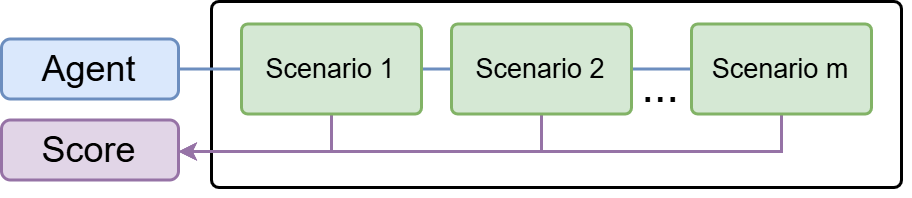
\includegraphics[width=0.6\textwidth]{images/methodology/tool_steps_reduced.png}
    \caption{Summarised benchmark process of \benchmark evaluating one agent}
    \label{fig:tool-steps} 
\end{figure}

In \benchmark, a \textbf{scenario} is defined as a five-tuple 
\[(\text{Network}, \text{Profile}, \text{Modifications}, \text{Eval}_{idx}, ep_{len})\]
where network is the topology description of a power grid, profile shows the changes of the generators and loads in the network over a range of time, and modifications are changes over the grid, e.g. scaling of specific generators or reducing the capacity of a line (explained more in depth in Section \ref{ssec:implementation-grid-mod}). $\text{Eval}_{idx}$ is the set of starting indices to use for a single scenario run $i\in\text{Eval}_{idx}$. Each agent starts running from index $i$ until $i + ep_{len}$ for each run. Thus $ep_{len}$ defines the episode length. This tuple design was chosen to make each scenario reproducible and to differentiate between scenarios. If any component of this tuple is changed, the resulting scenario has a different scope and complexity. Altering the network can result in a new grid topology that differs greatly in size and complexity. This affects the difficulty of stabilising the power grid during the simulation. When the profile or grid modification is changed, power generation and consumption might become much easier or harder for the \ac{rl} agent to manage. Furthermore, the score is influenced by the length of the episode. The longer the episode, the more difficult it is to maintain a stable grid. Additionally, the starting indices impact the difficulty of maintaining grid stability in a scenario. For example, energy consumption is higher in the evening than during the day because most people are at home using electricity.

\benchmark also enables the user to use custom agents. Those agents must potentially be trained before they can be evaluated. Hence, \ac{rl} agents get the following six-tuple
\[(\text{Network}, \text{Profile}, \text{Modifications}, \text{Train}_{idx}, \text{Eval}_{idx}, ep_{len})\]
which additionally has the $\text{Train}_{idx}$ information. $\text{Train}_{idx}$ and $\text{Eval}_{idx}$ define the indices to start training or evaluation from, respectively. They do not have any overlapping indices, as the agent must be trained on different indices compared to the evaluation indices. This tests the agent's performance on unknown grid states. Although the agent is trained on a scenario, it is evaluated on each evaluation index separately.
The used technologies and the implementation of these steps are explained further in Chapter \ref{ch:implementation}.



\section{Metrics and Evaluation}\label{sec:metrics-eval}
To evaluate the quality of the agent, data from each run is collected in the form of different grid metrics. These metrics are then aggregated into a final score that is the output of the benchmark. Each metric can be classified into one category that the benchmark focusses on.

\subsection{Metric Categories}\label{ssec:metric-categories}
The metrics are categorised into five different groups, which are demonstrated in Figure \ref{fig:categories-bm}. These categories are used to calculate the score of a run, which will be explained further in Section \ref{ssec:score-calc}. Each category contains a variety of metrics for evaluating the agent's performance. Table \ref{tab:metric_categories} in the appendix lists all the metrics in each category.

The metrics in the \textbf{overload mitigation} category measure how well the agent avoids line overloads. Examples of these metrics include the timesteps without overloads and the number of overloaded transmission lines. Depending on the settings chosen by the user, the overload mitigation metrics can also include $N-1$ overload metrics. This setting is discussed further in Section \ref{sec:int-processes}.
In the \textbf{voltage violation mitigation} category, metrics determine how well the agent mitigates bus voltage violations. These include, for example, metrics that measure the maximum or mean percentage of voltage deviation from the nominal values at the buses in a timestep. 
The \textbf{survival} category contains only one metric that indicates how many timesteps the agent kept the power grid in a stable, converged state. A state is considered converged when the power flow equations can be successfully solved. Convergence does not necessarily imply operational safety, hence the inclusion of voltage violations, overloads and other operational metrics in \benchmark. 
The \textbf{costs} category focuses on metrics that determine operational costs, such as frequency of actions on substations, power losses, and load shedding (where loads receive insufficient or no electricity). 
Finally, the \textbf{computational performance} category evaluates runtime, as well as CPU and memory usage. Some metrics have two parts, one measuring the average value of the metric over the course of the episode, and the other measuring the worst observed value. In Section \ref{sec:metrics-description} in the appendix there is a more detailed explanation for each metric, and which metrics are measured by their average and worst value. 

\begin{figure}[htp]
    \centering
    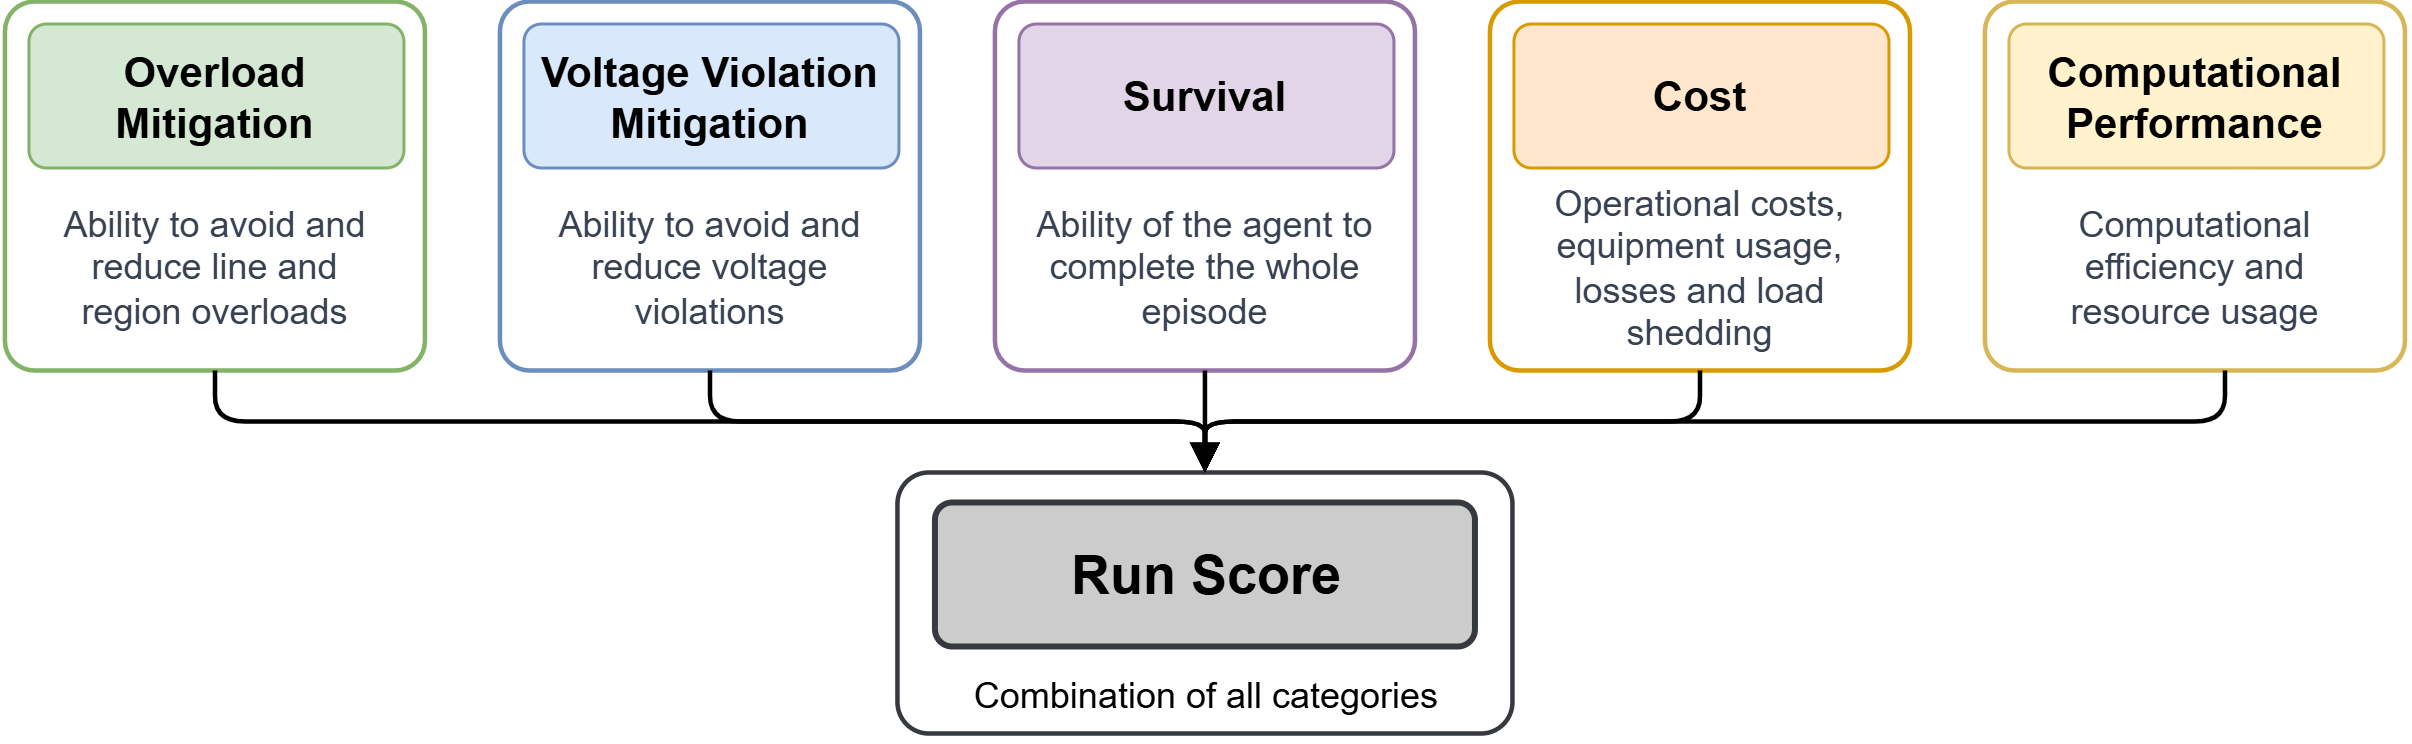
\includegraphics[width=0.99\textwidth]{images/methodology/benchmark_categories.png} 
    \caption{Evaluation categories of \benchmark that form the run score}
    \label{fig:categories-bm} 
\end{figure}

\subsection{Score Calculation}\label{ssec:score-calc}
Each metric has a different numerical range. Therefore, the scoring function normalises every metric value to a score between 0 and 100, where 0 represents the worst score and 100 represents the best score. This is done by defining a worst value \(x_{\mathrm{worst}}\) and a best value \(x_{\mathrm{best}}\) for each metric. Values between these two bounds are mapped linearly to the interval \([0, 100]\), while values outside the bounds are clipped to either 0 or 100.

Equations \eqref{eq:linear_metric_score_increasing} and \eqref{eq:linear_metric_score_decreasing} define the scoring function for the two possible cases. Equation \eqref{eq:linear_metric_score_increasing} applies to metrics where larger values are better, while Equation \eqref{eq:linear_metric_score_decreasing} applies to metrics where smaller values are better. For example, for the number of survived timesteps in an episode, the best value is the episode length \(ep_{\mathrm{len}}\), while the worst value is 0. In contrast, for the total number of timesteps with voltage violations, this relation is reversed. The best value is 0, while the worst value is \(ep_{\mathrm{len}}\). Section \ref{sec:metrics-description} in the appendix contains the exact values of \(x_{\mathrm{worst}}\) and \(x_{\mathrm{best}}\) for each metric.

\begin{equation}
s(x) =
\begin{cases}
0, & x \leq x_{\mathrm{worst}}, \\[4pt]
100 \cdot \dfrac{x - x_{\mathrm{worst}}}{x_{\mathrm{best}} - x_{\mathrm{worst}}},
& x_{\mathrm{worst}} < x < x_{\mathrm{best}}, \\[8pt]
100, & x \geq x_{\mathrm{best}},
\end{cases}
\qquad
\text{for } x_{\mathrm{worst}} < x_{\mathrm{best}}.
\label{eq:linear_metric_score_increasing}
\end{equation}

\begin{equation}
s(x) =
\begin{cases}
100, & x \leq x_{\mathrm{best}}, \\[4pt]
100 \cdot \dfrac{x_{\mathrm{worst}} - x}{x_{\mathrm{worst}} - x_{\mathrm{best}}},
& x_{\mathrm{best}} < x < x_{\mathrm{worst}}, \\[8pt]
0, & x \geq x_{\mathrm{worst}},
\end{cases}
\qquad
\text{for } x_{\mathrm{worst}} > x_{\mathrm{best}}.
\label{eq:linear_metric_score_decreasing}
\end{equation}

Each metric and category has a weight. These weights are used to emphasise specific metrics or categories, or to allow users to omit those that are not important for their goals. For example, the computational performance category might not be as significant as other categories if a lot of resources are available and the user's goal is not to optimise resource usage. 
These weights are used to calculate an aggregated score for each run. Equation \eqref{eq:run_score} shows these calculations. For each category $c \in \mathcal{C}$, a \textbf{category score} $S_c$ is calculated. 
This is defined by the weighted average over all metrics $m \in \mathcal{M}_c$ of the category $c$, using their scores $s_m$ and weights $w_m$. The aggregated \textbf{run score} $S_{\text{run}}$ is then defined by the weighted average of all category scores $S_c$, using the category weights $w_c$. If the simulation of a run did not finish at least one iteration of the full episode, each of the category scores and the run score is assigned a value of zero. 
This happens when the simulation starts with a non-converging grid state that directly ends the simulation. If the run ended at timestep $t < ep_{len}$ due to non-convergence, then all metrics that depend on the episode length use $t$ as the new episode length. For the survival metric however, the score uses $t$ as the number of survived iterations and calculates what percentage of the full episode was reached, as a penalty for not reaching the episode's end.

\begin{equation}
S_{\text{run}} = \frac{\displaystyle\sum_{c \in \mathcal{C}} S_c \cdot w_c}{\displaystyle\sum_{c \in \mathcal{C}} w_c}
\qquad 
\text{with } S_c = \frac{\displaystyle\sum_{m \in \mathcal{M}_c} s_m \cdot w_m}{\displaystyle\sum_{m \in \mathcal{M}_c} w_m}
\label{eq:run_score}
\end{equation}

Since each scenario consists of one or multiple runs, the aggregated \textbf{scenario score} is defined as the average over all run scores of the runs of the scenario. As the final experiment score, the \textbf{total score} is defined by the average of all scenario scores from the evaluated scenarios in the experiment.

\subsection{Design Rationale}
The \benchmark categories have been chosen to cover multiple significant aspects of a stable power grid operation. It is not enough to simply check whether the agent survived the entire episode. It is necessary to observe other metrics, which is why the categories cover a broad field of power grid operation. 

Furthermore, the weights assigned to each category and metric allow the user to emphasise the important aspects of their research. For example, if the main goal of improving the \ac{rl} agent is to mitigate overload and voltage violations, then these categories must be given a higher weight. Conversely, if a research group has plenty of computational resources, computational performance may be irrelevant, in which case this category can be set to a lower weight or even zero weight. 

To make the benchmark output transparent, the user receives a set of statistics showing all these scores. It consists of the average for each metric, category and scenario, as well as individual scores for each scenario. This facilitates analysis of weak spots and provides a more thorough output if the user aims for deeper insights. The aggregated score provides a quick overview of which agent performs better on average. Section \ref{sec:result-format} showcases the output formats and options for visualising them.

\section{Evaluation Protocol}\label{sec:evaluation-protocol}
Users have many options to consider when preparing and executing evaluations using \benchmark to evaluate custom agents. 
Firstly, a selection of scenarios needs to be made. This step is the most important, as each scenario tests the agent's ability to solve these grids and provides a review of its performance. The more diverse the scenarios, the better the benchmark's coverage is. Additionally, the selected scenarios can be used to track improvements to the agent over different versions, or for comparison with others. 

To create a thorough set of scenarios, the first step is to create and test a scenario with a \textbf{do-nothing} agent. It runs very quickly, as it does not need to select any actions, which makes it easier to cover a wide range of profile indices. This agent assesses the general difficulty of the scenario, but more significantly, it identifies specific indices that are harder in maintaining grid stability. The lower the benchmark score for these indices, the more it shows that a simple agent that does not interact with the environment is insufficient. Furthermore, it is important to decide which evaluation metrics should carry more weight than others, or which to leave out completely. This depends solely on the user's optimisation goal. With the help of the do-nothing agent, a couple of indices in the created scenario are revealed to be the most complex to solve. 

To further filter these indices, the \textbf{greedy agent} is used. If this agent also struggles to reach high scores, it means that the indices require more training or planning to stabilise and ensure the safety of the power grid. Once these steps have been completed for multiple scenarios covering diverse situations, the selection of scenarios and evaluation indices is complete.

After these steps, the custom agent has to be tuned and trained for each scenario (see Section \ref{sec:agent-integration} for more information), using the remaining profile indices that are not included for evaluation. Once the training is completed, the custom agent is evaluated by running the benchmark pipeline. The pipeline and its tasks are explained in Section \ref{sec:int-processes}.
    \chapter{Implementation}\label{ch:implementation}
This chapter describes the implementation of \benchmark and the technologies used to realise the concepts introduced in Chapter \ref{ch:methodology}. While the methodology focused on the design decisions and theoretical foundation of the benchmark, this chapter examines how these ideas are put into practice in more detail. It explains the internal processing pipeline, how scenarios are constructed, how agent integration works, and how results are presented.



\section{Internal Processes}\label{sec:int-processes}
When running \benchmark, configurations in the form of YAML files are passed as input. These define the scenarios for evaluation, what agent to use (see more in Section \ref{sec:agent-integration}), which task to do and other settings. Listing \ref{lst:yaml-configs} shows a minimal working example for the configuration files. There, the IEEE 14-bus and 30-bus power grids are chosen, with the first and 100th profile indices for evaluation (see more on the Power Grids and Profiles in Section \ref{ssec:implementation-grid-profiles}). In the main configuration, the one on the right, a greedy agent is chosen that runs the tasks "Run" and "Evaluate" with four CPUs and with $N-1$ power flow calculation in the simulations. The greedy agent is configured with a reward function that minimises the maximum line loadings in $N-0$. The reward function is explained in more detail in Section \ref{sec:agent-integration} and the exact information on benchmark usage and what to set in the YAML files is shown in the documentation\footnote{\documentation} of the benchmark tool.

\begin{listing}[htp]
\centering
\footnotesize
\begin{minipage}{0.85\textwidth}
    \begin{minipage}[t]{0.32\textwidth}
    \begin{minted}{yaml}
- category: IEEE
  case: 14
  indexes:
    values: [0, 99]
- category: IEEE
  case: 30
  indexes:
    values: [0, 99]
    \end{minted}
    \end{minipage}
    \hspace{0.1\textwidth}
    \begin{minipage}[t]{0.47\textwidth}
    \begin{minted}{yaml}
name: "Greedy Agent"
agent_type: Greedy
scenario_files:
  - some/path/scenario.yaml
output_dir: some/path/output
task: ["Run", "Evaluate"]
n_cpu: 4
env_config:
  nminus1: True
  reward:
    max_line_loading_nminus0: 1.0
    \end{minted}
    \end{minipage}
\end{minipage}
\caption{Example YAML files for the benchmark settings: scenario (left) and main configuration (right)}
\label{lst:yaml-configs}
\end{listing}

Figure \ref{fig:bm-tasks} shows the processes inside \benchmark, which include the run and evaluation tasks that were previously discussed. Inside these configurations, the tasks that are set tell the benchmark tool what to do in the current run. Depending on these settings, either the main benchmark pipeline starts, or the results of already generated scores are presented (more on this in Section \ref{sec:result-format}). 

There are multiple processes that can be run inside the benchmark pipeline, each of which is run on all the chosen scenarios in the configuration. Before benchmarking starts, each scenario must be prepared. This is an important step for custom user agents, as training takes place here. This is discussed further in Section \ref{sec:agent-integration}. Once this step is complete, the agent runs through all scenarios separately. This is achieved using the PPTopoGym environment, which was presented in Section \ref{ssec:grid-ctrl-systems}. In this environment, the agent selects actions that are then executed, and the resulting state and reward are calculated using pandapower and a customisable reward function. If $N-1$ power flow calculation is set, like in Listing \ref{lst:yaml-configs}, then PPTopoGym performs these calculations using pandapower. The run either ends when the episode length is reached or when the power grid exceeds its limit and does not converge. Information about the run is always saved in the output folder, hence the user is able to skip this step, if they already have run data. This data is used for two final tasks. The evaluation task involves replaying the run data and gathering metrics to create the actual score. These metrics are then transformed into scores ranging from 0 to 100, which are then aggregated to produce a final score, as explained in Section \ref{ssec:score-calc}. Metrics for runtime per iteration, CPU usage and memory usage are measured during the run process. The evaluation data is then saved in JSON files, which document all the metrics and score pairs gathered for each scenario. These files are loaded by the result presenters shown in Section \ref{sec:result-format} to provide users with an overview of the benchmark output.

Another task that uses the run data is the replay task. In this task, the agent's actions are repeated in PPTopoGym, with plots and tables being created at each step of the episode. At the end of the task, these plots and tables are combined into an HTML file, which is then saved locally. This file provides a step-by-step visualisation of the actions chosen by the agent and their impact on the power grid in one run of a scenario. More about this output is discussed in Section \ref{ssec:replay-data}.

\begin{figure}[htp]
    \centering
    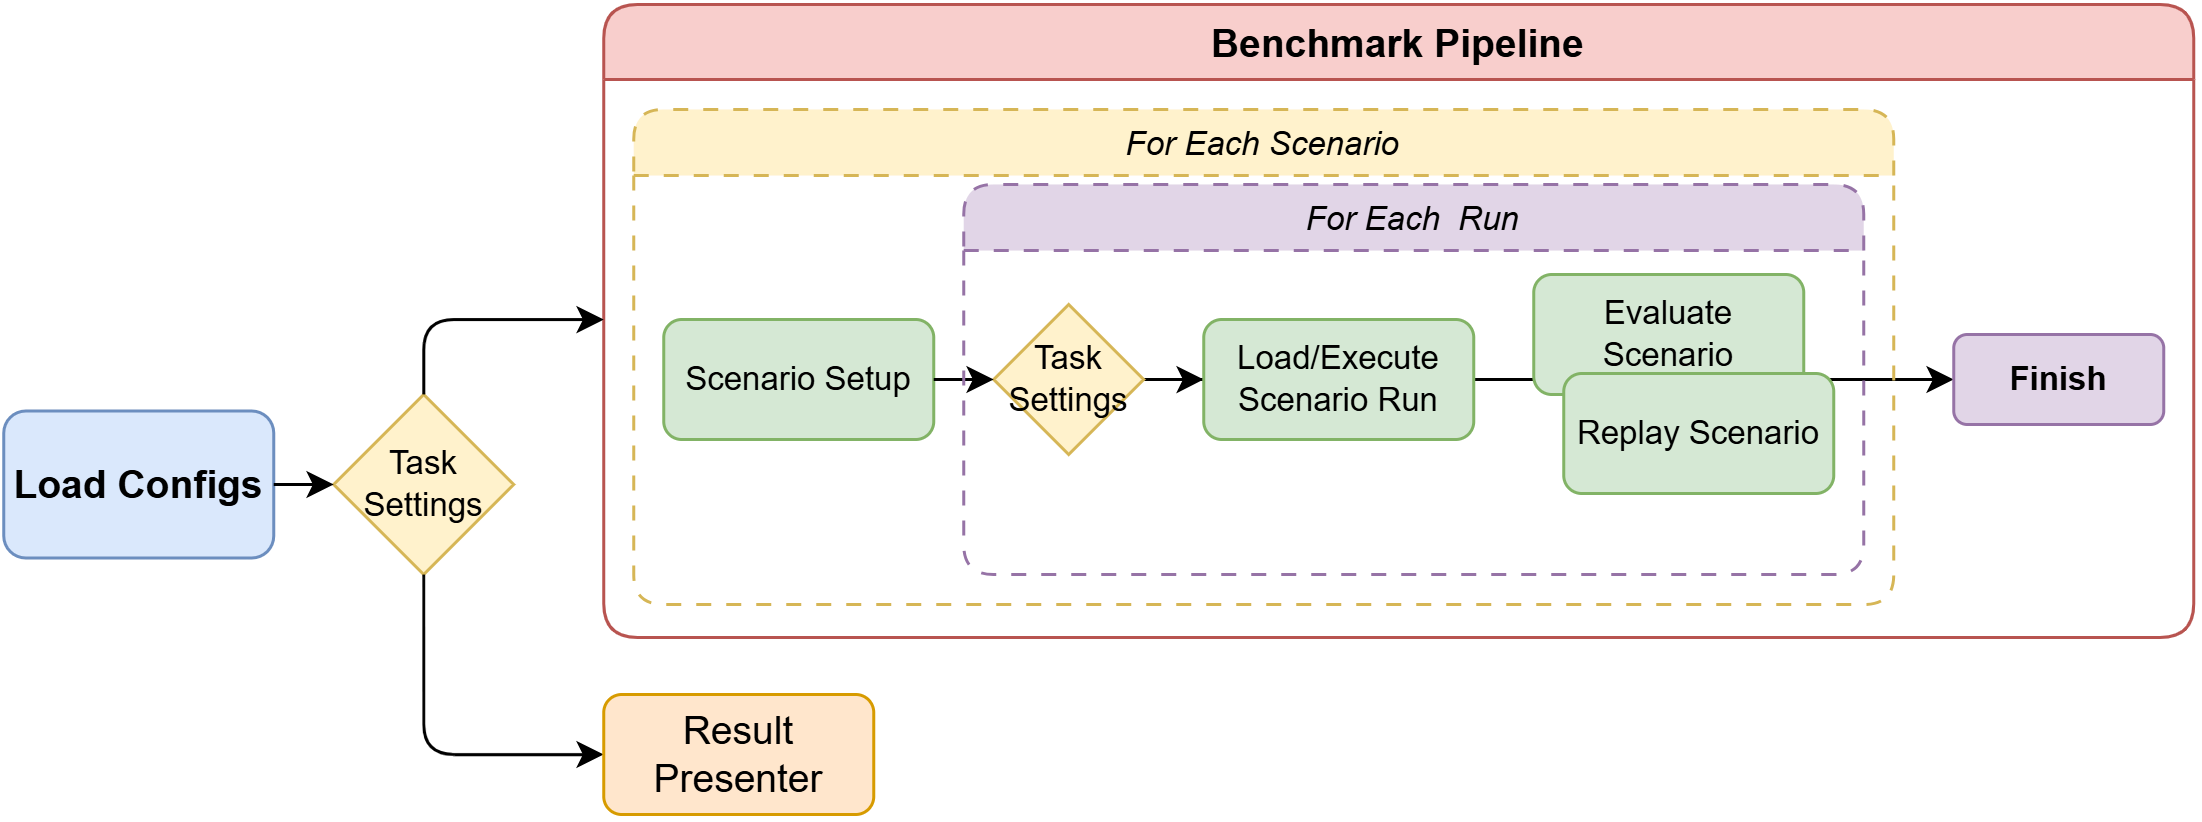
\includegraphics[width=0.95\textwidth]{images/implementation/benchmark_pipeline.png}
    \caption{Activity diagram showing all possible processes of \benchmark}
    \label{fig:bm-tasks} 
\end{figure}



\section{Scenario Implementation}\label{sec:implementation-scenarios}
This section describes how the scenarios introduced in Section \ref{sec:benchmark-structure} are implemented in \benchmark. It first presents the possible power grids and profiles that form the basis of a scenario. It then introduces the grid modifications that can be applied on top of these grids and profiles to increase scenario diversity and difficulty. Together, both define the building blocks to allow users to configure a wide range of scenarios.

\subsection{Grid and Profiles}\label{ssec:implementation-grid-profiles}
As discussed in Section \ref{sec:benchmark-structure}, each scenario consists of a power grid, a profile, and network modifications. Currently, the power grid benchmark supports IEEE test cases and data from SimBench. 

The IEEE test cases are introduced in Section \ref{ssec:power-benchmark}, as standardised and realistic power grid models. Figure \ref{fig:exp-grids} shows the 14-bus and 30-bus grids from the IEEE test cases, which are used in the experiments in Chapter \ref{ch:experiments}. They contain buses (shown as the circles), loads and generators (depicted as green and red triangles), transmission lines and transformers (represented as lines, with transformers drawn thicker), and the external grid (illustrated as the yellow rectangle). While pandapower does not have any substation modelling, PPTopoGym supports it by adding substation information to a pandapower grid \cite{pptopogym}. External grids in pandapower are modelled as voltage sources with a defined voltage magnitude and angle, which are represented as slack nodes in the power flow calculation and thus balance the power in the grid \cite{pandapower}.

SimBench is a benchmark dataset of German power grids, which provides realistic grids and profiles with 15-minute resolution over the course of a full year. It offers thirteen different power grids, each with three variants, as well as a variety of profiles (e.g. for photovoltaic or wind generation) \cite{simbench}. Additionally, SimBench data supports the format used in pandapower \cite{simbench}, making it a fit usage in PPTopoGym. 

The IEEE test cases have been selected because they have been used in many previous studies for benchmarking power grids, and because they are realistic. The SimBench dataset has been selected to complement the limited number of IEEE test cases and to provide more variety and benchmark coverage. Both datasets model realistic grid topologies ranging from small to large power grids, with profiles always loaded from the SimBench dataset.

\subsection{Grid Modification}\label{ssec:implementation-grid-mod}
To create a broader variety of scenarios for testing the agents, \benchmark offers a few network modifications that users can configure. These modifications make scenarios more or less complex in terms of grid stability, depending on the scaling. This allows the agent to be pushed to its limits more effectively, enabling a deeper assessment of its strengths and weaknesses and creating edge cases for evaluation. The modifications include load and generator scaling, maintenance events, and line and transformer capacity scaling.

\paragraph{Load and Generator Scaling.} Load and generator scaling redistributes the consumption or generation of electricity. This allows scenarios to be created where most of the electricity comes from a few generators or where a couple of loads require much more electricity than the rest. This maintains the total amount of electricity generated and consumed from the original data, but shifts the distribution to be more or less extreme.

\paragraph{Maintenance Events} Another modification is the introduction of maintenance events, which simulate real-world situations in which grid components are turned off due to maintenance or outages caused by long-term usage. These components include lines, switches, transformers and generators. This feature is similar to the maintenance in the \ac{l2rpn} benchmark explained in Section \ref{sssec:l2rpn}. Scenarios involving maintenance are more challenging as electricity must flow through longer paths or generation relies on fewer generators. Furthermore, to make the simulation more realistic, transmission lines or transformers, that reached a loading of 150\% of their physical limit, get set into maintenance. This simulates edges of the grid that were pushed over the limit and were destroyed in the process. When that happens, they need to be fixed, hence the maintenance event. They will not be usable for the rest of the episode. 

\paragraph{Line and Transformer Capacity Scaling} The capacity of lines and transformers is scalable, to configure the maximum allowed current of lines and transformers. This adjusts how fast the physical limit of the grid edges is reached. This is done by scaling the \textit{max\_i\_ka} value, which is the maximum allowed current in kiloamperes \cite{pandapower_docs}. If the value is reduced, the lines and transformers reach their thermal limits faster. This is relevant in grids where a specific line or transformer is particularly important. When the capacity of this component is reduced, the agent must distribute the electricity to other components. Otherwise the downscaled component may fail due to exceeding its limit for too long.



\section{Agent Integration}\label{sec:agent-integration}
\benchmark offers two baseline agents and allows users to implement their own. The first baseline is a \textbf{do-nothing agent}, which never applies any action to the power grid. The second is an exploitative \textbf{greedy agent}, which evaluates the available actions in the current state and selects the one yielding the highest reward.

The reward signal is provided by the underlying PPTopoGym environment from the work of \citet{pptopogym} and is therefore not part of the benchmark contribution of this thesis. However, the function was extended into a configurable, metric-based form used for the experiments shown in Chapter \ref{ch:experiments}. Equation \ref{eq:reward_func} defines this reward. If the power flow does not converge in the current step, the reward is the constant penalty $r_{\mathrm{fail}}$. Otherwise, it is computed as a weighted sum of metric scores. Each metric $m \in \mathcal{M}$, with $\mathcal{M}$ being the set of reward metrics in use, corresponds to a value measured from a grid feature and is weighted by $w_m$. The scoring function $s_m$ maps the measured value to $[0,1]$ using a worst-case and a best-case reference value, clipping results that fall outside this interval. Normalising by the sum of the absolute weights yields a reward in $[0,1]$. The available metrics and reference values partly coincide with the benchmark metrics of Section \ref{sec:metrics-eval}. In the benchmark configuration, the user sets which reward metrics to use and how much weight they have. Section \ref{ssec:reward-metrics-description} lists the configurable options for the reward and what their worst-case and best-case reference value, for the score mapping, are set to.

\begin{equation}
\text{reward} =
\begin{cases}
r_{\mathrm{fail}}, & \text{if the power flow does not converge},\\[2.2ex]
\displaystyle \frac{\sum_{m \in \mathcal{M}} w_m \, s_m}{\sum_{m \in \mathcal{M}} \lvert w_m \rvert}, & \text{otherwise}.
\end{cases}
\label{eq:reward_func}
\end{equation}

Another type of agent is custom agents brought by the user. These, just like the greedy agent, use the customisable reward function from Equation \ref{eq:reward_func}. In order to create such a custom agent, a couple of inputs and outputs need to be implemented. The \texttt{BenchAgent} class within the project defines this structure. Custom agents must be a subclass of the \texttt{BenchAgent} class. The necessary functionalities are shown in Figure \ref{fig:agent-pipeline}. The custom agent is embedded in the benchmark pipeline discussed in Section \ref{sec:int-processes}, where it is connected to the benchmark setup and scenario execution. For the setup, a \ac{rl} agent needs to be initialised and then trained for each scenario. During training, the agent produces checkpoints which save the trained state after multiple iterations. It is possible to use these to either skip the training process and load an existing checkpoint, or ensure reproducibility with the same state as a trained agent. Once the agent has been set up for one scenario, it is used to decide on actions during evaluation runs. After these runs have been saved, the agent can be evaluated, or the actions can be replayed. Additionally, \benchmark offers a \texttt{RayAgent}, a child class of \texttt{BenchAgent} that provides multiple RLlib-implemented functionalities. RLlib is a \ac{rl} library built on top of the Ray framework. It offers a unified interface and implementation of \ac{rl} algorithms, such as \ac{ppo} \cite{rllib}. The \texttt{RayAgent} class simplifies the process of creating a new agent, as only agent initialisation needs to be implemented. 

\begin{figure}[htp]
    \centering
    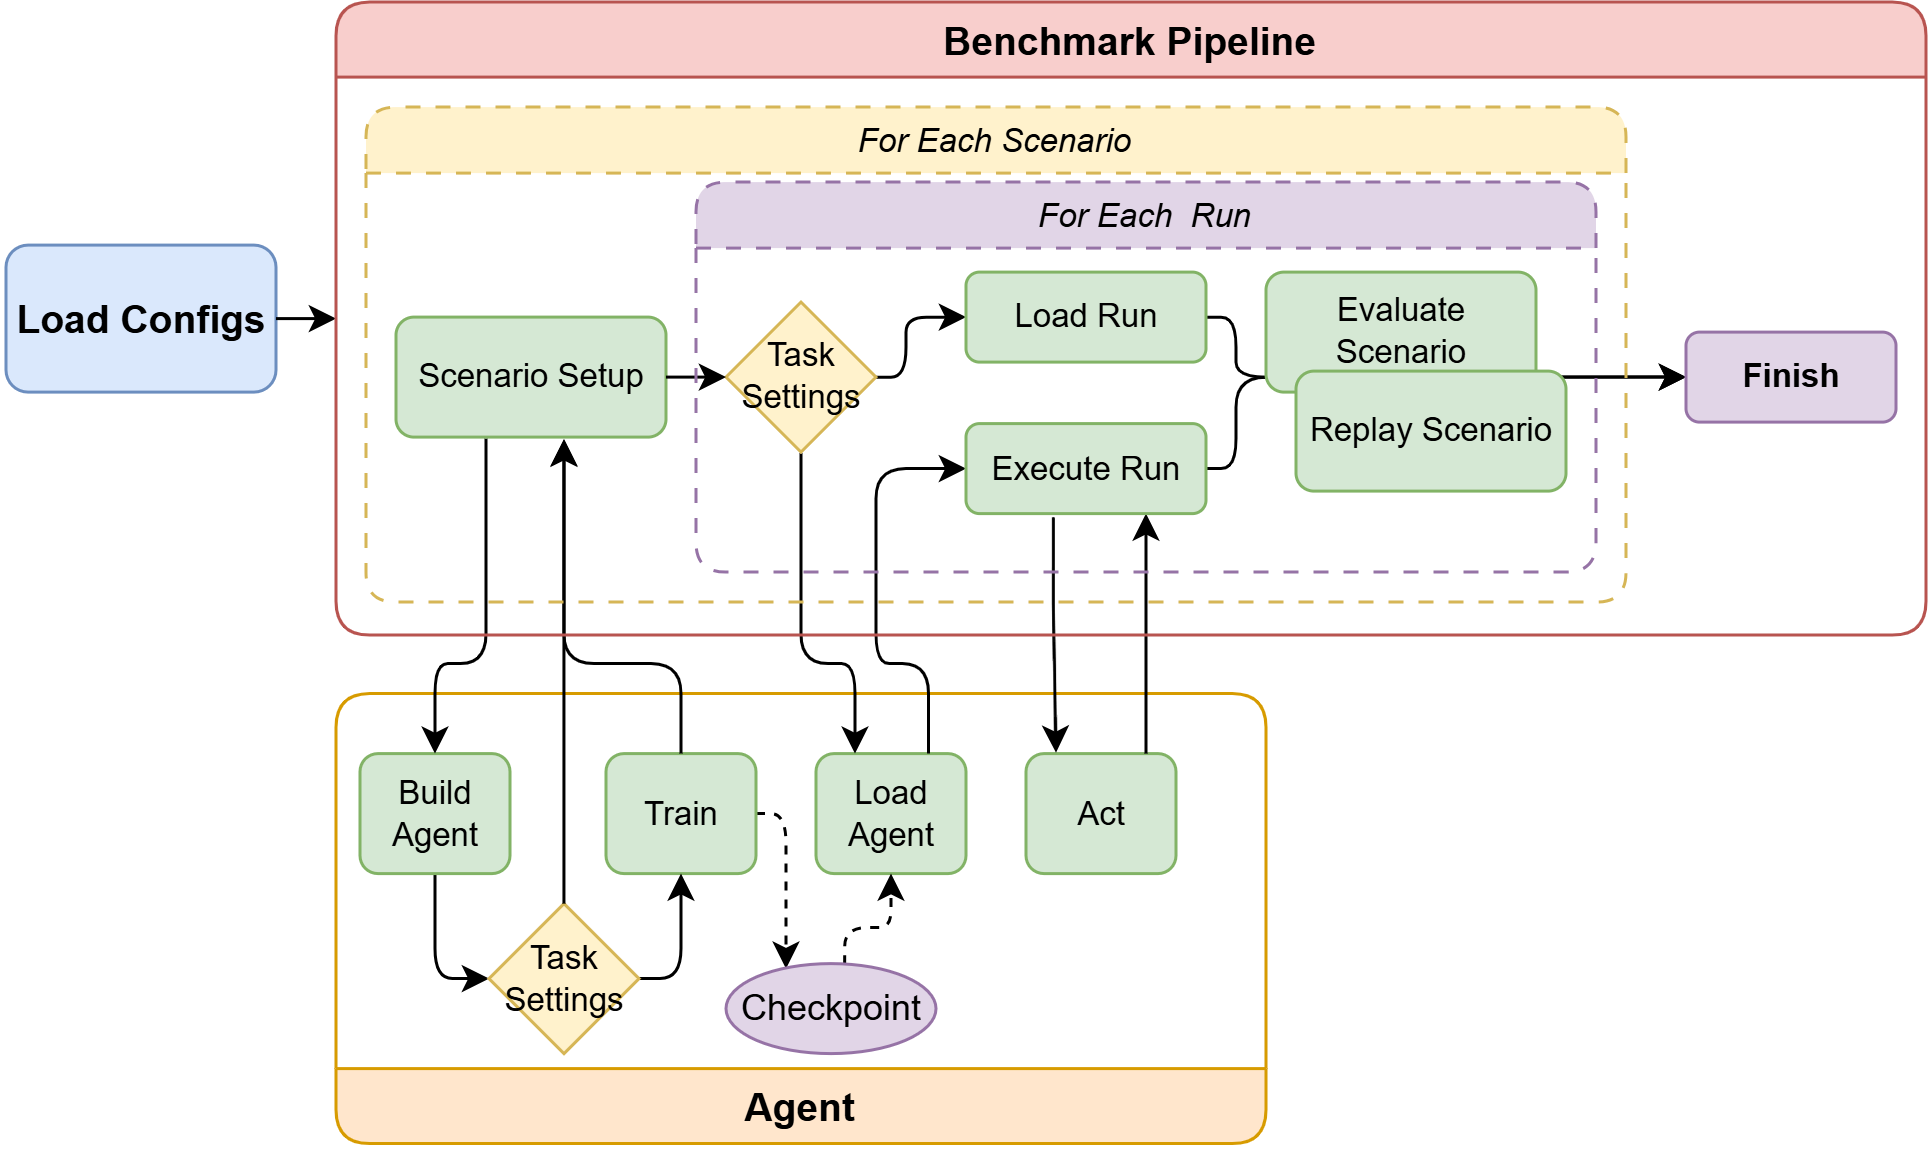
\includegraphics[width=0.95\textwidth]{images/implementation/pipeline_agent.png}
    \caption{Interaction between the benchmark pipeline and the agent}
    \label{fig:agent-pipeline} 
\end{figure}

\ac{rl} agents do not optimise every parameter during training. Hyperparameters, such as the learning rate, layers in a neural network, or the batch size, are set during initialisation and never changed. To find the perfect settings for these, \benchmark offers the \texttt{BaseTuner} class. This class provides an interface for custom tuning classes that optimise the hyperparameters of custom agents. A child class of \texttt{BaseTuner} is \texttt{OptunaTuner}, which simplifies the implementation of custom Optuna tuning for the user's agent. Optuna is a hyperparameter optimisation framework \cite{optuna}. The user defines the value ranges for each hyperparameter in the custom child class of the \texttt{OptunaTuner}. Optuna then creates the search space, carries out the experiments, and returns the optimal hyperparameters efficiently and reproducibly \cite{optuna}.



\section{Result Format}\label{sec:result-format}
This section demonstrates how the evaluation output is visualised and which tools are offered to do so. The format of the results and the information shown affect the quality and focus of the feedback provided to the user. Some important information is not immediately apparent and requires the correct visualisation to be seen. Furthermore, the benchmark gathers a lot of information, which would be time-consuming to read and analyse. The following paragraphs will present how the raw output, which contains a lot of information, is summarised and visualised to provide an in-depth overview of the agent's performance using textual or visual feedback.

\subsection{Raw Output}\label{ssec:raw-output}
Once an agent has been evaluated, the resulting metrics and scores are saved in a JSON output. The output for each scenario looks like the example in Listing \ref{lst:result-json}. Each run of the scenario is saved in the \texttt{results} array. All the metrics for each of these runs are saved as value-score pairs. For example, for the metric \texttt{timesteps\_without\_overload} of the first result in the example, there were zero timesteps with any overloads over the full episode with 96 timesteps, giving the best score of 100. Some metrics have multiple values, such as the total number of lines overloaded per timestep in $N-0$ power flow (shown here as \texttt{\seqsplit{total\_lines\_overloaded\_timestep\_nminus0}}), for which the value-score pairs for each iteration are saved. For these metrics, the mean and worst scores are used to aggregate the scores into a single score. This is saved in \texttt{resulting\_scores}, and the measured values for these scores are in \texttt{resulting\_values}. When only one value is measured for a metric, such as timesteps without overload, there is only one resulting score and value. To understand the scoring from 0 to 100, the worst and best possible values are stored in \texttt{scoring\_range}.
Once all the metrics have been listed inside a category, the category score is saved. This is done for each category in the same way, unless a category has a weight of zero. In that case, as can be seen in the computational performance category of the example, no metrics are measured or saved, and only a category score of zero is written. Finally, the index, episode length and the aggregated score are saved for each run.

\begin{listing}[htp]
\begin{minted}[fontsize=\scriptsize, breaklines, baselinestretch=0.6]{json}
{
    "name": "IEEE14_original",
    "network_category": "IEEE",
    "scenario_config": ".../ieee14.yaml",
    "results": [
        {
            "overload_mitigation": {
                "timesteps_without_overload": {
                    "values": [[96.0, 100.0]],
                    "resulting_scores": 100.0,
                    "resulting_values": 96.0,
                    "scoring_range": {"wp_val": 96.0, "bp_val": 0.0}
                },
                ...
                "total_lines_overloaded_timestep_nminus0": {
                    "values": [[0.0, 100.0], [0.0, 100.0], ...],
                    "resulting_scores": {"mean": 100.0, "worst": 100.0},
                    "resulting_values": {"mean": 0.0, "worst": 0.0},
                    "scoring_range": {"wp_val": 15.0, "bp_val": 0.0}
                },
                ...
                "category_score": 89.64805329153604
            },
            "voltage_violation_mitigation": { ... },
            "survival": {
                "survived_iterations": {
                    "values": [96.0, 100.0],
                    "resulting_scores": 100.0,
                    "resulting_values": 96.0,
                    "scoring_range": {"wp_val": 0.0, "bp_val": 96.0}
                },
                "category_score": 100.0
            },
            "costs": { ... },
            "computational_performance": {"category_score": 0.0},
            "index": 1920,
            "episode_length": 96,
            "total_score": 83.70538341352134
        },
        ...
    ]
}
\end{minted}
\caption{Exemplary output for the do-nothing baseline agent.}
\label{lst:result-json}
\end{listing}

After gathering the data for each scenario result, \benchmark creates a \textit{statistics.json} file, which summarises the total and scenario results. Listing \ref{lst:statistics-json} illustrates an example of what this might look like. It presents information about the final aggregated score, the average category score, and the number of metrics gathered across all scenarios. In this case, there were 15 scenarios, each measuring 27 different metrics, for a total of 810 metrics measured across all 30 runs. Additionally, the same information is shown for each scenario. 

\begin{listing}[htp]
\begin{minted}[fontsize=\scriptsize, breaklines, baselinestretch=0.6]{json}
{
  "total_score": 64.8135,
  "category_scores": {
    "overload_mitigation": 69.1923,
    ...
  },
  "metrics_average": {
    "timesteps_without_overload": {"score": 20.6598, "value": 19.8333},
    "total_lines_overloaded":     {"score": 99.1886, "value": 32.0},
    ...
  },
  "metrics_gathered": {
    "amount_of_metrics": 27,
    "amount_of_scenarios": 15,
    "total_amount_metric_gathered": 810
  },
  "scenarios": {
    "IEEE14_original": {
      "scenario_score": 52.7911,
      "category_scores": {
        "overload_mitigation": 89.7843,
        ...
      },
      "metrics_average": {
        "timesteps_without_overload": {"score": 0.0,    "value": 0.0},
        "total_lines_overloaded":     {"score": 100.0,  "value": 0.0},
        ...
      },
      "metrics_gathered": {"amount_of_metrics": 27, "total_amount_metric_gathered": 81}
    },
    "IEEE14_upscale_gen0_downscale_rest": {
      "scenario_score": 40.4203,
      ...
    },
    ...
  }
}
\end{minted}
\caption{Exemplary \textit{statistics.json} output for the do-nothing baseline agent.}
\label{lst:statistics-json}
\end{listing}

JSON is a human-readable output format, but it quickly becomes overloaded with text and information when dealing with large amounts of data. Moreover, to make the data more compact, not all the data is labelled or explained. For example, the saved values are value-score pairs, which are not explained anywhere. The main purpose of this output format is to save the evaluation on the machine for later analysis.

\subsection{Textual Feedback}\label{ssec:textual-feedback} 
\benchmark offers two forms of textual feedback, which share the same information. One creates a report that is printed in the console and saved in Markdown format. An example of the console printing is demonstrated in Listing \ref{lst:textual-report}. This shows the results for a do-nothing agent that went through 15 different scenarios and a total of 30 runs across all scenarios. 
Initially, this information is presented, including the average general score and average category scores. Then more specific information is displayed, such as average scores and measured values for specific metrics, and how often these were gathered throughout the experiment. Additionally, the average scenario scores and the number of runs are shown. Finally, the report goes through each scenario, providing average scores for the categories and metrics. Alternatively, there is an interactive reporter where the user selects which of this information should be printed in the console using console inputs. The textual feedback form is useful for quickly obtaining a thorough overview of the average values and scores across multiple levels within the benchmark. It produces output similar to JSON files, but in a more readable and compact format. 

\begin{listing}[htp]
\begin{minted}[fontsize=\scriptsize, breaklines, baselinestretch=0.6]{text}
============================================================
BENCHMARK REPORT: DN
============================================================
Agent:               DoNothing

OVERVIEW
----------------------------------------
Average Score:       64.8135
Total Scenarios:     15
Total Results:       30
Category · overload_mitigation:          69.1923
...

METRICS OVERVIEW
----------------------------------------
Metric                                    Avg Score  Avg Value  # Gathered
timesteps_without_overload                  20.6598    19.8333          30
total_lines_overloaded                      99.1886    32.0000          30
...

SCENARIO OVERVIEW
----------------------------------------
Scenario                                Avg Score  # Gathered
IEEE14_original                           42.7911           3
IEEE14_upscale_gen0_downscale_rest        40.4203           2
...

------------------------------------------------------------
Scenario: IEEE - IEEE14_original
------------------------------
Configuration:  .../ieee14.yaml
Network Category:    IEEE
Average Score:       42.7911
Category · overload_mitigation:          89.7843
...

Metric Overview
------------------------------
Metric                                    Avg Score  Avg Value  # Gathered
timesteps_without_overload                 100.0000     0.0000           3
total_lines_overloaded                     100.0000     0.0000           3
...
\end{minted}
\caption{Exemplary benchmark report for the do-nothing baseline agent.}
\label{lst:textual-report}
\end{listing}

\subsection{Visual Feedback}\label{ssec:visual-feedback}
Another type of result is graphs and plots. These enable users to instantly identify trends, distributions and comparisons. This makes them especially valuable for determining which scenarios or categories an agent is struggling with and for comparing multiple agents against each other.

\subsubsection{Result Plots}
The output of the plotting tool is created using Matplotlib, a Python library for creating publication-quality static plots and graphs \cite{matplotlib}. Additionally, as an alternative to Matplotlib, the plotting tool offers Plotly, which is another Python library for creating interactive plots and graphs \cite{plotly}. The same plots are created for both Matplotlib and Plotly. These include five overview plots containing all scenarios, and three plots showing how the agent performed in each scenario.

Figure \ref{fig:eval-plots} illustrates an example of all the overview plots. It contains a heatmap presenting the score for each category in each scenario, the distribution of scores across all runs in each scenario, the distribution of category scores, and a comparison of scores across scenarios and their individual runs. These plots help to visualise the strengths and weaknesses of the agent in each category or scenario. In the presented example, it can be seen that the agent performs very well in terms of overload mitigation, but struggles with voltage violations. Furthermore, the agent performs much better in the \texttt{IEEE14\_upscale\_load0\_downscale\_rest} scenario, in which the 14-bus power grid from the IEEE test cases is used and modified so that load 0 has an increased power demand.

Figure \ref{fig:eval-scenario-plots} demonstrates an example of the individual scenario plots. These plots include a radar chart of the category scores, the category scores themselves, and the total score for each run. The plots again show, that voltage violation was the agent's weakness and overload mitigation its strength for this scenario. Additionally, they demonstrate that the category scores and the average score in the first and third runs, as shown in Figures \ref{fig:eval-category-bar} and \ref{fig:eval-score-index}, are higher than in the second scenario run.

\subsubsection{Webapp}
Another supported visualisation is an interactive web app with Streamlit. Streamlit is a Python framework for building lightweight web applications that focus on data presentation \cite{streamlit}. Figure \ref{fig:webapp-screenshots} depicts screenshots of an example result from a web app created for an experiment involving a do-nothing agent. The web app combines textual and visual reports similar to those demonstrated previously. It begins with an overview, shown in Figure \ref{fig:webapp-overview}, where the user sees a summary of how well the agent performed overall. This includes information about the average score, the number of scenarios and the total number of runs, as well as the average scores for each category. The scenario overview and scenario details then provide information about each scenario, including the average score, the number of runs, and the average category scores. This allows for individual scenario analysis to identify which ones were more difficult to solve. 
Finally, the section on individual results goes over each run of the currently selected scenario in the section on scenario details, presenting the average score and the score over categories and metrics. These metrics and scores provide the lowest level of detail and are used to analyse specific runs in greater depth. The web app shows the same plots for each scenario as in Figures \ref{fig:eval-scenario-plots} and \ref{fig:eval-plots}, using either Plotly or Matplotlib. In this way, the web app provides in-depth analysis of specific scores or runs and visual representations using plots from the plotting tool. This makes it easier to analyse strengths and weaknesses, as well as provide an overview of the agent. Users are able to perform both superficial and general performance analyses, as well as conduct more in-depth analysis to identify the root causes of problems. 

So far, the result format has focused on feedback for single-agent experiments, but the web app additionally has an option to start a comparison between two agents. This is built similarly to the standard web app, but it displays the results side by side, as depicted in the example in Figure \ref{fig:comparison-webapp-screenshots}. Additional features include demonstrating differences in scores and plotting category scores next to each other for direct comparison of the two results. This form of feedback is useful for comparing two agents. It provides a general comparison using the aggregated scores and a specific comparison for individual runs or scenarios using generated plots displayed side by side. This makes it easy to see which agent has stronger or weaker features, making the decision between the two agents easier.

\subsection{Replay Data}\label{ssec:replay-data}
One form of feedback that does not use evaluation data to generate its output is data from the replay task. As explained in Section \ref{sec:int-processes}, this data is created by replaying the run data and constructing plots of the state of the power grid at each timestep. The plots are created using Plotly, and the output is an HTML page containing all the information in one page. The page contains two graphs at the beginning, both of which illustrate the power grid from different perspectives. Below these, there is a section demonstrating all the tables from the pandapower network (lines, buses, generation, etc.). Figure \ref{fig:replay-graphs} shows how the two graphs make up this page.

Figure \ref{fig:network-graph} shows a network graph that visualises the grid's topology and indicates how close each component is to its operational limit. For example, the colours green to red to black on the transmission lines illustrate how much they are overloaded. Red or black indicates that the line is overloaded by more than 100\%. The same is done for transformers, if any exist. For the buses, the normalised bus voltage is presented to indicate how much it deviates from the operational safe range. Green indicates normal voltages, while shades of blue or red demonstrate that the voltages deviate too far below or above the nominal values. The darker the colour shades, the worse the voltage violations. Additionally, this graph shows which generator produces the most power and which load consumes the most, highlighting them in a darker shade of their respective colour.

The action graph, as shown in Figure \ref{fig:action-graph}, focuses more on the actions taken by the agent. It demonstrates which bus was affected by the agent's action, such as the topology changes that were made. An example of this is demonstrated in Figure \ref{fig:action-graph-zoomed}, which is the same grid as in Figure \ref{fig:action-graph}, just zoomed in. This figure shows how one bus was split and which lines were connected to which of the new buses. Moreover, it illustrates how the load, labelled \textit{L2} in this plot, was connected to the substation on the right-hand side of the figure. As the plots are created using Plotly, it is easy to zoom in and analyse the new grid connections made after an agent's action.

This output is an analysis tool that helps users to understand the actions of agents and their impact. If a user, for example, is unsure why the agent received a low score in a specific category, the option to use the replay data exists. This helps identify the behaviour or actions that caused the agent to perform poorly in that category. Furthermore, this output is useful for identifying challenging scenarios to use for benchmarking. It provides a visual analysis, demonstrating for each step of an episode which lines are the bottlenecks, which generators produce more, and which loads require more power. Unlike the others, this output uses different data and has a different goal. It analyses past runs to provide insight into the grid and the agent by showing actions, bus splits and how the grid reacts to new states.
    \chapter{Experiments}\label{ch:experiments}
In order to answer the research question posed by this thesis, a series of experiments was conducted using \benchmark to evaluate and compare three agents of increasing complexity: a do-nothing agent, a greedy agent, and a trainable \ac{ppo} agent. Rather than testing a single grid configuration, the experiments cover a broad range of scenarios, including unmodified standard test grids, intentionally destabilised topologies, gradually intensified stress conditions, and pure performance tests. This enables a general ranking of the agents to be obtained, as well as a detailed analysis of their individual strengths and weaknesses across different metrics and categories.

The chapter is structured into three main parts. Section \ref{sec:experiment_setup} describes the experimental setup, including the selected scenarios, the configuration of the benchmark categories, the two baseline agents and the custom PPO agent, as well as the expectations derived from this setup. Section \ref{sec:experiment-results} then presents the results obtained from running all experiment scenarios, first providing an overall comparison and then breaking the results down by experiment category. Finally, Section \ref{sec:exp-analysis-interpretation} analyses and interprets these results in depth. It explains recurring patterns in the agents' behaviour and summarises the findings into a strength and failure profile for each agent.

\section{Experimental Setup}\label{sec:experiment_setup}
This section describes the setup used to conduct the experiments in this thesis. Section \ref{ssec:experiment-scenarios} first introduces the experiment categories and the specific scenarios contained within them, along with the configuration of the benchmark's category weights. Section \ref{ssec:baseline-agents} then presents the two baseline agents used in all experiments, the do-nothing and greedy agents presented in Section \ref{sec:agent-integration}, together with the defined reward function that is used in the experiments. Section \ref{ssec:custom-agent-setup} then describes the architecture, training process and tuning of the custom \ac{ppo} agent, which is compared against the two baselines. Finally, Section \ref{ssec:exp-expectation} formulates the expected outcomes for each experiment category based on the experiment design decisions presented in this section.

\subsection{Experiment Scenarios}\label{ssec:experiment-scenarios}
The experiments cover different fields important in grid stability and operation. All the experiments are categorised into two groups. The \textbf{grid operation} experiments range from a normal run of unmodified IEEE grids, to diverse scenario coverage by different grid modifications and finally to a stress test, where difficulty is increased by multiple levels of scaling of a grid modification. The category of \textbf{performance-only} contains one experiment, which compares runtimes and computational resource usage between agents.

\subsubsection{General Setup}
Each of the experiments is run with a whole day as episode length. Using the data from SimBench as profiles, this gives 96 iterations for one episode, as the time series values are provided for every 15 minutes. It is important to note that although SimBench provides profiles for renewable generation as well, only conventional generation and load profiles are used throughout the experiments in this thesis. This choice was made to isolate the effect of the individual grid modifications discussed in Section \ref{ssec:implementation-grid-mod} on the agents' performance, without introducing the additional, weather-driven variability and intermittency associated with renewable generation. Furthermore, while SimBench also provides larger and more complex power grids, the grids used in this chapter were deliberately chosen to be less complex. This decision allows for a clearer overview of the agents' behaviour, as larger grids would be considerably more difficult to visualise and present within the scope of this thesis.

For all experiments, the 14-bus and 30-bus IEEE test cases are used as power grids. Figure \ref{fig:exp-grids} shows the two power grids, following the visual conventions introduced in Section \ref{ssec:implementation-grid-profiles}, and highlights the grid components that are modified in the experiments. In the figures, buses are drawn as small circles, while substations are drawn as bigger circles. Furthermore, it is visible that the 30-bus grid does not contain any transformers. The difference in size between the two grids is also visible from the figures, as the 30-bus grid has significantly more components, forming a more complex, interconnected grid than the 14-bus one.

Table \ref{tab:cat-weights-setup} shows the chosen weights of each benchmark category used for the evaluation of each experiment. For the grid operation experiments, the focus is on grid stability, hence \textit{computational performance} is left out of the evaluation. As for the performance-only experiment, the focus is opposite to that of the grid operation experiments, with only the \textit{computational performance} category being evaluated.

\begin{table}[htbp]
    \centering
    \caption{Benchmark Category Weights}
    \label{tab:cat-weights-setup}
    \begin{tabular}{lcc}
        \hline
        Category & Grid Operation & Performance-only \\
        \hline
        Overload Mitigation & 2 & 0 \\
        Voltage Violation Mitigation & 2 & 0 \\
        Survival & 3 & 0 \\
        Costs & 1 & 0 \\
        Computational Performance & 0 & 1 \\
        \hline
    \end{tabular}
\end{table}


\subsubsection{Chosen Scenarios and Experiments}
For each scenario, challenging test days are identified following the steps in Section \ref{sec:evaluation-protocol}. This was done by finding profile days on which the do-nothing agent achieves a benchmark score of about 50 and the greedy agent scores lower, i.e. days where neither inaction nor the locally optimal action suffices for a high score. The benchmark score is set up with the category weights shown in Table \ref{tab:cat-weights-setup}, using the weights from grid operation. In the following paragraphs the exact scenario selection process is explained. Table \ref{tab:scenarios-setup} shows all chosen scenarios over every experiment. It also explains which profile days were used and which grid components were modified. 

\paragraph{Standard Analysis.}
The first experiment category looks at the standard 14-bus and 30-bus from the IEEE test cases. This test shows the first overall comparison between the agents, with a normal power grid that does not have any extremes or modifications. It compares the performance in normal grid operation. As seen in Table \ref{tab:scenarios-setup} under the scenarios \textit{14B\_ORIG} and \textit{30B\_ORIG}, for the 14-bus grid, three profile days were chosen, and for the 30-bus grid, one profile day was chosen. For the 14-bus grid there were more challenging scenarios, while the unmodified 30-bus grid did not have many difficult days, so the one with the lowest benchmark score was chosen.

\paragraph{Diverse Scenario Coverage Analysis.}
This experiment explores how \benchmark can be used, to cover more diverse scenarios. With grid modification, different cases in the 14- and 30-bus power grids are created. This experiment examines how the agents behave with more extreme cases, where there is a factor making the grid less balanced and adding instability to it. 

One case in this experiment is the shifting of the generation of power more towards a single generator. This makes one generator produce more energy, while the others produce less. Another case shifts the consumption more to a single load to create a less balanced grid. For both generation and load scaling the sum of generation or consumption is preserved to the value in the original power grid. If generation or consumption is concentrated at a single point, larger, unevenly distributed power flows result, which make the grid less robust to withstand disturbances and making stabilisation more difficult.
To find the right trials, each one of the generators and loads from the grids in the 14- and 30-bus IEEE test case has been scaled in separate experiments. Finally, the generator and load with the biggest impact on destabilising the grid have been selected for this experiment. This has been done again like in Section \ref{sec:evaluation-protocol}, using the scores of the two baseline agents. The chosen generators and loads and how much they are scaled are noted in Table \ref{tab:scenarios-setup} and their position in the grid is highlighted in Figure \ref{fig:exp-grids}.

The other cases of grid modification focus on limiting power grid components for the grid with 30 buses. The modifications include maintenance events in generation or transmission lines, or downscaling the capacity of transmission lines.
The transmission lines, that had the highest loading during the standard unmodified network runs, have been chosen to be downscaled or put under maintenance. By limiting or disabling these bottleneck components of the power grid, the power needs to be redirected into other lines, testing the agent's ability to plan when components have issues. In the case of the generator maintenance, the generator near the external grid has been put into maintenance. As a result, the external grid has to be used much more. The problem is that the generator under maintenance is connected to four lines, while the external grid is only connected to two lines, making it a bigger challenge to supply the power without overloading the lines. For these modifications again Table \ref{tab:scenarios-setup} documents the chosen components and Figure \ref{fig:exp-grids} shows their location in the grid.

\paragraph{Stress-Test Analysis.}
For this experiment category, the scalable scenarios from the diverse scenario experiment are used. For each of the cases, different levels of scaling are evaluated, increasing the difficulty of each power grid gradually. Each of these tests contains three levels of scaling. First, a light scaling modifies the grid just slightly, affecting the difficulty very little. The next scaling uses exactly the same trials shown in the second experiment, which is right in the middle between the light and heavy scaling. For the heavy scaling the difficulty is increased the most, making it very hard to maintain a stable power grid. The scalable scenarios include the load, generator and line capacity modification tests. These trials test how each agent reacts to increasing stress, and if the different scaling of difficulty affects the scoring system. The exact scaling levels are documented in Table \ref{tab:scenarios-setup}, which shows for each scaling level the exact multiplier.

\paragraph{Performance Analysis.}
For this experiment the same scenarios as the standard analysis experiments are chosen. In this experiment, only the computational performance of the greedy and \ac{ppo} agents is evaluated. It tests the runtime and computational resource usage of both agents, working with the 14- and 30-bus grid. The goal is to illustrate, how these two agents compare in performance, measuring this on two different grid sizes, which hold different degree of complexity in connected components. 


\subsection{Baseline Agents}\label{ssec:baseline-agents}
As already covered, the experiments contain different categories that cover diverse scenarios to do a deep analysis. Each of these is evaluated and compared across multiple agents, always using the same three agents. 
The do-nothing agent is a reference point that indicates how demanding a scenario is without intervention. In some cases, the current network topology does not need much or any changes, as the power grid stays stable. 
But in more complex cases, like imbalanced power generation or demand, or bottleneck components that overload quickly, an agent that acts and changes the topology is needed. The greedy agent is chosen as a second baseline agent. It evaluates the available topology actions and chooses the one that yields the highest reward. 
For the reward, the customisable reward discussed in Section \ref{sec:agent-integration} is utilised. It punishes non-convergence in the power grid with a negative reward and looks at the metrics of maximal line loading and the present number of overloaded lines, both in $N-0$ power flow. The exact values set for the experiment are seen in Table \ref{tab:reward_settings}. The reward is deliberately kept simple and focuses only on two objectives, reducing line overloads in $N-0$ and avoiding non-convergence. Other metrics are intentionally excluded, even though \benchmark evaluates them. This allows the experiments to show how a narrow reward definition affects the benchmark scores. 

\subsection{Custom Agent Setup}\label{ssec:custom-agent-setup}
Choosing the best action for the current step is not always ideal. The best action for the current state might not be the best action for the stability of the grid. Both baseline agents do not have any component that plans for the future timesteps. In more complex power grids, an agent that is trained for its topology and profile can be more advantageous. For this reason, the third agent is a custom agent, implemented also as a test on how to use \benchmark as a developer, and to see how trained agents would compare to other untrained agents like the do-nothing and greedy agents.

The chosen custom agent is a \ac{ppo} agent that uses a \ac{gnn} as a policy encoder. It is implemented in RLlib as a subclass of the RayAgent described in Section \ref{sec:agent-integration} and follows the PPTopoGym reference agent \cite{pptopogym}. The encoder consists of a configurable stack of GINEConv layers, i.e. the edge-feature-aware variation of the \ac{gin} \cite{ginPaper}, which aggregates the embeddings of neighbouring nodes together with features of the connecting edges through a sum operation followed by an \ac{mlp} \cite{ginePaper}. The depth and width of the GINEConv layers are selected during hyperparameter optimisation for each scenario. These layers process the node features (voltage magnitude and angle at buses) and edge features (line and transformer loadings) of the power grid graph \cite{pptopogym}. As a result, each bus of the power grid is represented by an embedding generated by the GINEConv layers. The bus embeddings are then aggregated into a single embedding representing the entire power grid using a configurable graph-pooling operation, which is also selected during hyperparameter optimisation. Finally, the graph embedding is passed through a neural network with two heads, which create two outputs. The first head produces the action logits, which give one preference score for each action from the action space. The higher the score, the more preferable the action is for the grid state. During training, an action is sampled from the resulting probability distribution to encourage exploration, whereas during evaluation the action with the highest score is selected. The second head returns a value estimate, predicting the expected cumulative reward from the current state onwards.

The hyperparameters cover the architecture of the \ac{gnn} encoder and the fully connected head as well as the algorithmic parameters of \ac{ppo}, such as batch sizes, learning rate and clipping parameters. A complete listing and description of the parameters is given in Table \ref{tab:ppo-hparams}. Their optimisation is implemented using a customised child class of the OptunaTuner, presented in Section \ref{sec:agent-integration}. For each scenario the agent is first tuned over multiple trials and then trained with the tuned hyperparameters for a maximum of 3000 iterations, with early stopping if the best mean episode reward does not improve for 1000 consecutive iterations. Table \ref{tab:training-results} shows the results of the training for each scenario. The values shown are measured from the average cumulative reward over a full episode for the best training iteration. As each episode has 96 timesteps and the reward function per timestep has a maximum of one, the highest achievable cumulative reward is 96. As the penalty for non-convergence is -2, this is also the lowest cumulative reward. In some scenarios the \ac{ppo} agent almost reached the highest cumulative reward and in general the agent performed well in the 30-bus scenarios. In the 14-bus scenarios, however, it got some high values and some low values, even one close to the worst possible cumulative reward (for the highly scaled generator). 

\ac{ppo} is an established algorithm for grid topology control that combines naturally with a \ac{gnn} encoder. This allows the agent to exploit the topology of the power grid rather than operating on a flattened state vector. Training on individual load and generation profile episodes enables the agent to learn a policy that maps the current grid state directly to a switching action. This means that at runtime, the policy can directly decide one action. By contrast, greedy agents must simulate every candidate action at every time step to find the one with the highest reward. This makes the greedy agent slower and more computationally heavy during runtime. 

\subsection{Experiment Expectations}\label{ssec:exp-expectation}
Since the scenarios have been selected so that the greedy agent scores lower than the do-nothing agent, the relative ordering of the two baselines is fixed by design. Adding the custom agent introduces an additional element to the comparison: the effect of preparation through training. As the \ac{ppo} agent is tuned and trained to select actions that take future value into account, it is expected to achieve higher scores than both baseline agents. In simpler scenarios where the baselines already perform well, this difference is likely to be small. However, in more complex scenarios, the anticipatory behaviour of the \ac{ppo} agent should provide a clear advantage. As the reward only covers $N-0$ overloading and non-convergence, the agent is expected to excel in these two metrics in particular.

In the cost category, the metrics that evaluate executed actions are expected to favour the do-nothing agent, since an agent that never intervenes incurs no switching costs. However, this is just an advantage for this category, rather than an indication of effective operation. The outcome between the greedy agent and the \ac{ppo} agent is less clear. The greedy agent re-evaluates all candidate actions at every time step, so it may switch frequently. A trained policy, on the other hand, is more likely to settle into a stable topology and maintain it, resulting in lower costs. However, the reward used for training contains no cost component, so the \ac{ppo} agent has no motivation to minimise the number of actions and may act just as frequently as the greedy agent.

As for the grid modifications, they are expected to make grid stability more challenging to achieve, resulting in lower overall scores. The stress tests should gradually increase in difficulty across the scaling levels. While this increase should be reflected in the benchmark scores, the scores are not expected to drop in direct proportion to the amount of scaling. This is partly because only individual components are modified. As long as the surrounding lines still provide sufficient reserve capacity, the grid can absorb the additional stress to a degree, with few changes in the measured metrics. 

Finally, the decision-making process of the \ac{ppo} agent is expected to be faster than the action selection process of the greedy agent. As discussed in Section \ref{ssec:custom-agent-setup}, the greedy agent must compute the expected reward for each available action at each time step, whereas the policy of the PPO agent can choose an action directly. This advantage is expected to be more significant in the 30-bus grid, where the larger action space increases the number of required power flow calculations. However, the overall cost of the \ac{ppo} agent merely shifts into the preceding tuning and training phase.











\section{Results}\label{sec:experiment-results}
After running all the scenarios shown in the previous section, each agent has produced a set of scores for every scenario. This section presents these results, following the two experiment categories introduced in Section \ref{ssec:experiment-scenarios}. Section \ref{ssec:grid-operation-results} starts with an overall comparison of the total and category scores across all grid operation scenarios, before breaking the results down by the three individual experiments within this category: the standard test, the diverse scenario test and the stress test. It concludes with a look at the individual metric scores, to obtain a more granular view of the agents' performance. The performance-only experiment is then presented separately in Section \ref{ssec:perf-test-result}, comparing the runtime, CPU and memory usage of the greedy and \ac{ppo} agents across both tested grid sizes.

\subsection{Grid Operation Results}\label{ssec:grid-operation-results}
Table \ref{tab:agent_comparison} showcases the total score over all trials and their average category scores. Looking at the general overview, the \ac{ppo} agent achieved the highest scores, with the do-nothing agent having the second highest. The greedy agent on the other hand got lower scores in total. When looking at each category, the \ac{ppo} agent got higher scores than the other agents in all categories, except the costs category, where the do-nothing agent had the best score. Figure \ref{fig:bus-scores} documents the average category scores for the two power grids used in the experiments. Generally the scores are higher in the 30-bus grid. By contrast, for the costs category the \ac{ppo} agent and for the overload mitigation the do-nothing and greedy agents reach higher scores in the 14-bus grid.

\agentresulttable
  {Comparison of the agents in the grid operation experiments using the total score and category scores}
  {tab:agent_comparison}
  {
    Total Score & 58.20 & 41.25 & \textbf{64.86} \\
    \midrule
    Overload Mitigation & 53.90 & 51.44 & \textbf{73.22} \\
    Voltage Violation Mitigation & 41.54 & 30.21 & \textbf{56.85} \\
    Survival & 70.60 & 41.44 & \textbf{71.87} \\
    Costs & \textbf{62.89} & 42.34 & 43.09 \\
  }

Figure \ref{fig:exp-heatmap} offers a more detailed view over all trials, where the category scores of each agent for all the tested scenarios are shown. In general one can see that the agents achieved higher scores on average in the scenarios, where the 30-bus power grids were used. It is also visible, that the greedy agent has lower scores in general. Furthermore in the scenario with higher power generation scaling of generator 0 in the 14-bus grid, no agent survived any iteration of the episode. In Figure \ref{fig:metric-scores} the average scores over all metrics of \benchmark are shown. It is visible that the greedy agent never has the highest total score in any metric, while the \ac{ppo} agent has the highest score for most metrics. In the category of overload mitigation, survival and voltage violation mitigation the \ac{ppo} agent always has the highest score per metric. In the cost category the do-nothing agent achieves higher scores in all metrics, except the power loss metrics, where the \ac{ppo} reaches the highest values. These observed values match the results in average category scores, seen in Table \ref{tab:agent_comparison}.

\subsubsection{Standard Test Results} 
Table \ref{tab:exp_overview_standard} shows the aggregated results of the standard test, where the unmodified power grids with 14 and 30 buses from the IEEE test cases were looked at. This table has the same content as the general overview Table \ref{tab:agent_comparison}. However, the scores are only considering the averages of the test scenarios in the standard test experiment. Overall these specific results are similar to the total result obtained from all scenarios, just the \ac{ppo} agent performs worse in survival, where the do-nothing agent has the highest score. 

\agentresulttable
  {Comparison for the standard test experiment}
  {tab:exp_overview_standard}
  {
    Total Score & 61.32 & 41.17 & \textbf{65.00} \\
    \midrule
    Overload Mitigation & 63.15 & 62.91 & \textbf{80.93} \\
    Voltage Violation Mitigation & 44.60 & 33.13 & \textbf{58.06} \\
    Survival & \textbf{64.76} & 27.26 & 63.71 \\
    Costs & \textbf{80.81} & 55.49 & 50.87 \\
  }

Figure \ref{fig:scenario-scores-orig} shows a more detailed view over all the runs done in this experiment, and their category scores. In the 14-bus grid the agents perform with high scoring for overload mitigation and low scoring in survival and voltage violation mitigation. In the 30-bus grid the overload mitigation achieved lower scores for the do-nothing and greedy agents, while the scores for the do-nothing and \ac{ppo} agents increased for the survival and voltage violation mitigation. The greedy agent overall got low scores, except in overload mitigation in the 14-bus grid and in some runs of the costs category. In that category the do-nothing agent achieved constantly high scores, while the \ac{ppo} agent only got high scores in the 14-bus runs. 

\subsubsection{Diverse Scenario Results}
The diverse scenarios offer a variety of different grid modifications. The average scores over all scenarios and categories in this experiment can be seen in Table \ref{tab:exp_overview_diverse}. The results behave similarly to the overall average scores over all experiments, due to the \ac{ppo} agent having the highest scores in the total score and all categories except the costs, where again the do-nothing achieved the highest score by far.
\agentresulttable
  {Comparison for the diverse scenarios experiment}
  {tab:exp_overview_diverse}
  {
    Total Score & 64.15 & 45.70 & \textbf{76.19} \\
    \midrule
    Overload Mitigation & 51.86 & 46.66 & \textbf{79.41} \\
    Voltage Violation Mitigation & 50.76 & 39.77 & \textbf{71.96} \\
    Survival & 81.94 & 49.90 & \textbf{88.59} \\
    Costs & \textbf{62.14} & 43.05 & 41.05 \\
  }

Figure \ref{fig:tot-score-diverse} shows the final score distribution for each agent over all the scenarios covered in this experiment. Looking at the highlighted average values for all the agents, it shows that both scenarios in the 14-bus grid achieve scores below the average, while most of the scenarios in the 30-bus grid got scores above average. While the scores of the do-nothing and \ac{ppo} agents in the 30-bus grid remain relatively stable, the scores of the greedy agent fluctuate between higher and lower scores. In most scenarios the \ac{ppo} agent achieves higher scores, some even higher than the combined scores of the do-nothing and greedy agents, however, in the scenario of increased power consumption in the 14-bus grid the \ac{ppo} agent achieved a lower score than the other agents.

\begin{figure}[htp]
    \centering
    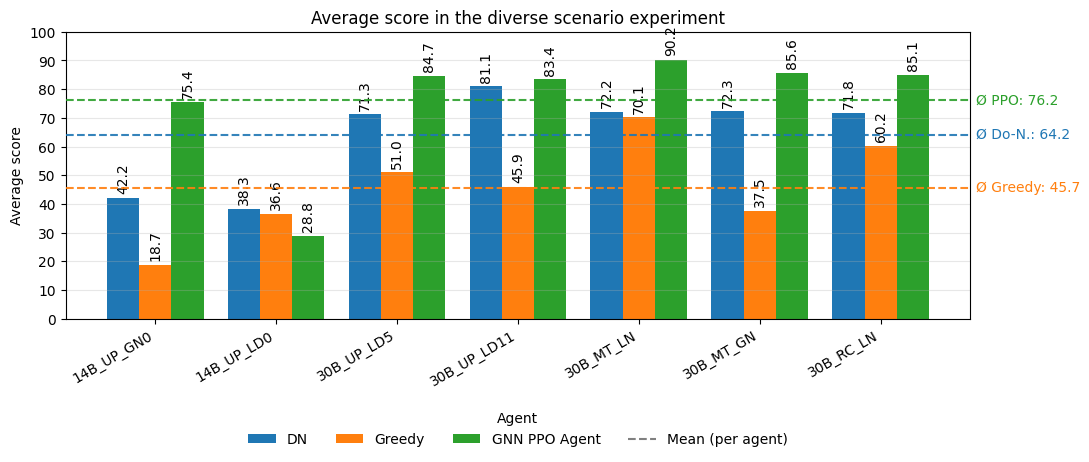
\includegraphics[width=1\textwidth]{images/experiments/total_scores/diverse_scenarios.png}
    \caption{Total score overview for the diverse scenario experiment, with average values of each agent}
    \label{fig:tot-score-diverse} 
\end{figure}

\paragraph{Modification of Generators and Loads.}
Figure \ref{fig:scenario-scores-14b-gnld-scaled} and \ref{fig:scenario-scores-30b-ld-scaled} show the results, for the power generation and consumption scaling experiment. For the load scaling in the 14-bus grid the three agents survived only in two of the three runs for more than one iteration. The last run got a score of zero, as no agent survived it. In the 14-bus scenarios the voltage violation mitigation of each agent is much lower than the scores of the 30-bus scenarios, while the overload mitigation scores are higher in the bus-14 scenarios. As for the survival, in all runs at least one agent has the maximum score of 100 or a score over 80, except for the second run in the scenario of increased load consumption in the 14-bus grid, where the scores are much lower. Also the \ac{ppo} agent usually has one of the highest scores in survival, but in all runs of the 14-bus increased load consumption scenario it reaches scores lower than the other agents. Also in the costs category this agent often has a low score, while the do-nothing agent achieved higher scores.

\paragraph{Modification through Maintenance and Line Capacity Reduction.}
Figure \ref{fig:scenario-scores-mnt} and \ref{fig:scenario-scores-rc} present the outcome of maintenance events and reducing the capacity of lines. The results are pretty similar in all three scenarios, with the \ac{ppo} agent achieving the best scores in all categories except costs, where the do-nothing got the highest scores. Just in the run of the line maintenance scenario the greedy agent has a maximum score, while performing with much lower scores in the other scenarios. In this scenario the do-nothing agent has a much lower value than usual in the costs category.

\subsubsection{Stress Test Results}
This experiment is made of three different experiments, with each different scaling of power generation, power consumption and line capacity. Table \ref{tab:exp_overview_stress} shows the average result over each of these tests. In general one can see, that the average scores, except in the line capacity scaling test, are much lower than in the previous experiments. In the generator and line capacity scaling trials the same pattern as in the other experiments can be seen, with the \ac{ppo} agent reaching the highest scores in all categories except the costs category. In the load scaling trial the do-nothing agent has the highest scores in all categories except of overload mitigation, where the \ac{ppo} agent has the highest score.

\begin{table}[htbp]
  \centering
  \caption{Comparison for the stress test experiment across all three scaling experiments}
  \label{tab:exp_overview_stress}
  \begin{tabular}{lrrr}
    \toprule
    Metric & Do-Nothing & Greedy & PPO \\
    \midrule
    \multicolumn{4}{l}{\textit{Generator Scaling}} \\
    Total Score & 33.39 & 17.30 & \textbf{40.21} \\
    Overload Mitigation & 54.35 & 43.20 & \textbf{59.02} \\
    Voltage Violation Mitigation & 13.19 & 10.70 & \textbf{21.23} \\
    Survival & 28.36 & 3.13 & \textbf{43.17} \\
    Costs & \textbf{46.99} & 21.20 & 31.65 \\
    \midrule
    \multicolumn{4}{l}{\textit{Load Scaling}} \\
    Total Score & \textbf{45.78} & 34.53 & 41.19 \\
    Overload Mitigation & 65.22 & 61.81 & \textbf{65.36} \\
    Voltage Violation Mitigation & \textbf{13.72} & 13.67 & 12.69 \\
    Survival & \textbf{48.15} & 26.62 & 40.39 \\
    Costs & \textbf{63.89} & 45.45 & 52.21 \\
    \midrule
    \multicolumn{4}{l}{\textit{Line Capacity Scaling}} \\
    Total Score & 72.00 & 58.79 & \textbf{84.88} \\
    Overload Mitigation & 44.32 & 51.78 & \textbf{78.23} \\
    Voltage Violation Mitigation & 62.71 & 25.75 & \textbf{90.59} \\
    Survival & \textbf{100.00} & 91.67 & \textbf{100.00} \\
    Costs & \textbf{61.91} & 40.28 & 41.43 \\
    \bottomrule
  \end{tabular}
\end{table}

\paragraph{Generator Stress Test.}
Figure \ref{fig:tot-score-gen-stress} shows the score distribution over all agents in the stress test experiment with the generator 0 from the 14-bus grid. In this stress test the agents did not survive any iterations for the highest generator scaling, thus leading to a low total score for each agent. While the do-nothing and greedy agent's scores decrease significantly over higher scaling, the score of the \ac{ppo} agent has a peak in the second highest scaling. Figure \ref{fig:scenario-scores-gn-stress} and \ref{fig:scenario-scores-14b-up-gn0} show also the average category score over each run for all scalings. For the highest scaling there are no plots, as the scores were zero. The increase of scoring for the \ac{ppo} is caused by a higher scoring in overload mitigation and survival for the second level of scaling. For the other agents the category scores lower between the first and second scaling. The greedy agent even reaches non-convergence for the third run of the second scaling.

\paragraph{Load Stress Test.}
Figure \ref{fig:tot-score-load-stress} shows the reached scores over all agents for the stress test experiment with the load 0 from the 14-bus grid. The scores of all three agents decline, as the scaling increases, with the do-nothing and \ac{ppo} agents having a strong decline after the first scaling. Figure \ref{fig:scenario-scores-ld-stress} and \ref{fig:scenario-scores-14b-up-ld0} show a more detailed scoring distribution of the individual runs in each scaling level. In the second and third level of scaling, no agent made any timestep converge during the third run of the scenario.

\paragraph{Line Capacity Stress Test.}
Figure \ref{fig:tot-score-line-cap-stress} shows the achieved scores over all agents in the stress test experiment with reduced capacity of lines in the 30-bus grid. In this experiment, the scores of each agent do not decline at all, remaining stable in their score ranges. Figure \ref{fig:scenario-scores-rc-stress} and \ref{fig:scenario-scores-rc} show the category score distribution over each level of line capacity reduction. The scores remain similar for the do-nothing and \ac{ppo} agents, while the greedy agent changes category scores, while still achieving similar average scores in each level. 

\subsection{Performance Test Results}\label{ssec:perf-test-result}
Table \ref{tab:exp_overview_performance} shows the results of the computational performance comparison between the greedy and \ac{ppo} agents. As explained in Section \ref{ssec:experiment-scenarios}, the do-nothing agent is not treated as a competing agent in this comparison because it serves as the computational reference baseline and performs no action-selection computation. The \ac{ppo} agent received a higher score than the greedy agent did in both the 14-bus and 30-bus scenarios, with scores close to the maximum in both grid sizes. The greedy agent on the other hand scored similarly in both grids, with a slightly higher score in the 30-bus grid.

\begin{table}[htbp]
\centering
\caption{Comparison of the agents in the performance test experiment}
\label{tab:exp_overview_performance}
\begin{tabular}{lrrr}
    \toprule
    Grid & Greedy & PPO \\
    \midrule
    14-bus & 63.65 & \textbf{98.68} \\
    30-bus & 66.67 & \textbf{99.34} \\
    \midrule
    Total & 65.16 & \textbf{99.01} \\
    \bottomrule
\end{tabular}
\end{table}

A closer look into the measured metrics of this experiment is illustrated in Table \ref{tab:exp_metrics_performance}. It demonstrates, that the \ac{ppo} agent has a faster runtime per timestep and a lower memory usage than the greedy agent, while the greedy agent always has a lower CPU usage than the \ac{ppo} agent. Notably, the runtime of the greedy agent increases considerably between the 14-bus and 30-bus grid, more than doubling, while the runtime of the \ac{ppo} agent stays nearly constant across both grid sizes. 

\begin{table}[htbp]
\centering
\caption{Measured average metric values for the performance test experiment}
\label{tab:exp_metrics_performance}
\begin{tabular}{llrr}
    \toprule
    Grid & Metric & Greedy & PPO \\
    \midrule
    \multirow{3}{*}{14-bus}
        & Runtime per timestep (s) & 3.98 & \textbf{1.32} \\
        & CPU usage (\%)           & \textbf{13.86} & 22.22 \\
        & Memory usage (\%)        & 27.22 & \textbf{11.08} \\
    \midrule
    \multirow{3}{*}{30-bus}
        & Runtime per timestep (s) & 8.47 & \textbf{1.44} \\
        & CPU usage (\%)           & \textbf{12.23} & 21.41 \\
        & Memory usage (\%)        & 26.61 & \textbf{11.55} \\
    \midrule
    \multirow{3}{*}{Total}
        & Runtime per timestep (s) & 6.23 & \textbf{1.38} \\
        & CPU usage (\%)           & \textbf{13.05} & 21.81 \\
        & Memory usage (\%)        & 26.91 & \textbf{11.32} \\
    \bottomrule
\end{tabular}
\end{table}





\section{Analysis and Interpretation}\label{sec:exp-analysis-interpretation}
This section provides a detailed analysis and interpretation of the experimental results presented in the previous section. 
First, Section \ref{ssec:metric-performance} takes a closer look at the individual metrics behind the category scores, explaining recurring patterns and problems in the agents' strategies. 
Building on this, Section \ref{ssec:influence-grid-size} examines how the size of the two utilised grid topologies affects the benchmark scores, independently of the specific grid modification applied. 
Section \ref{ssec:influence-modification} then discusses the effect of the individual grid modifications on scenario difficulty and the effects on the evaluated categories, using the do-nothing agent to isolate their impact. 
Section \ref{ssec:behaviour-stress} extends this analysis by examining the agents' behaviour under increasing stress levels for generator, load and line capacity scaling. 
Three representative runs are then examined in depth in Section \ref{ssec:case-studies} to explain notable differences between the do-nothing and \ac{ppo} agents. 
Section \ref{ssec:computational-performance} analyses the results of the performance test experiment, relating the measured runtime, CPU and memory usage to the architectural differences between the greedy and \ac{ppo} agents. 
Finally, Section \ref{ssec:agent-profiles} summarises all findings into a strength and failure profile for each agent, demonstrating how \benchmark can be used to systematically uncover both the capabilities and the shortcomings of \ac{rl}-based grid operation agents.

\subsection{Metric Performance}\label{ssec:metric-performance}
This subsection takes a closer look at the individual metrics evaluated by \benchmark, in order to explain the category-level scores discussed previously and to identify recurring patterns in the agents' strategies.

When looking at the metrics evaluated by \benchmark in Figure \ref{fig:metric-scores-overload} and \ref{fig:metric-scores-survival} one can see, that the \ac{ppo} agent achieved higher scores than the other agents in all metrics. This is due to the agent's goal in training, to reduce overloads in $N-0$ and to keep converging grid states. This aligns with the expectations formulated in Section \ref{ssec:exp-expectation}. However, the strategy chosen by the agent for some scenarios is problematic in real-world cases, as Figure \ref{fig:exp-grids-off} demonstrates for two scenarios in the 14- and 30-bus grid. To reduce the overloads of lines, the agent switches off the majority of the power grid, turning off every generator and only providing power to one load close to the external grid, by using the external grid as the only power source. This is a common problem with faulty reward functions, often called \textit{reward hacking} \cite{rewardHacking,openaiFaultyReward}. The agent tries to maximise its reward signal without achieving the intended goal for the decision problem. In this case the agent obtained a faulty reward, that only covers a part of important metrics for good power grid operation. It maximises overload mitigation and the avoidance of non-convergence, by making the problem easier to solve, disconnecting a majority of the power grid. However, this is not ideal for the actual problem of stable and ideal power grid operation, where the full power grid should work and receive power.

\begin{figure}[htp]
    \centering
    \begin{subfigure}[b]{0.53\textwidth}
        \centering
        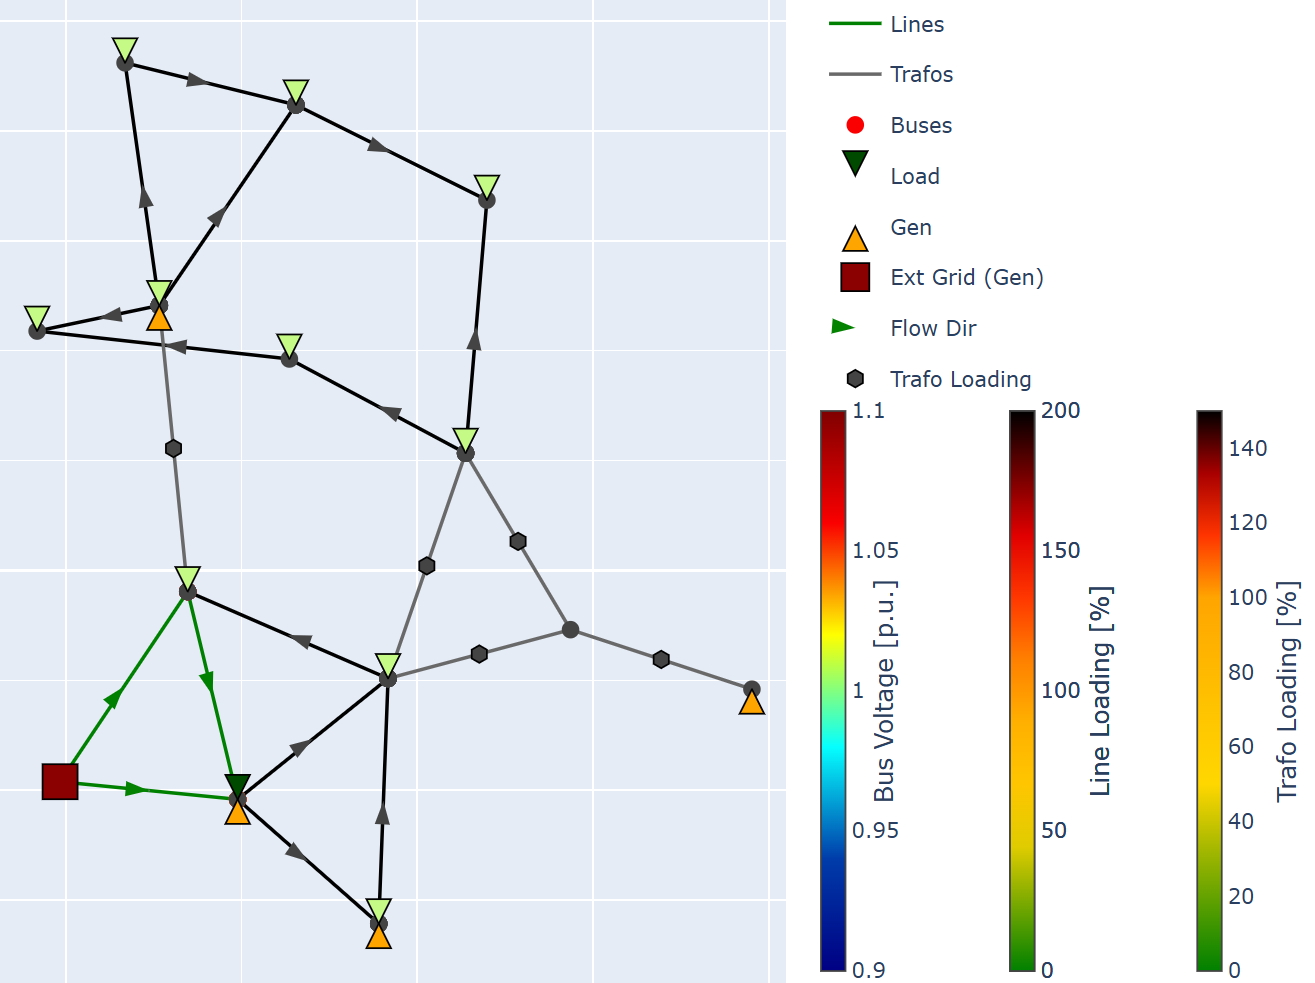
\includegraphics[width=\textwidth]{images/experiments/grids/14b_switched_off.png}
        \caption{Generator scaled 14-bus scenario, with every component disconnected, except the lines going to load 0 and 3}
        \label{fig:grid-14-off}
    \end{subfigure}
    \hfill
    \begin{subfigure}[b]{0.45\textwidth}
        \centering
        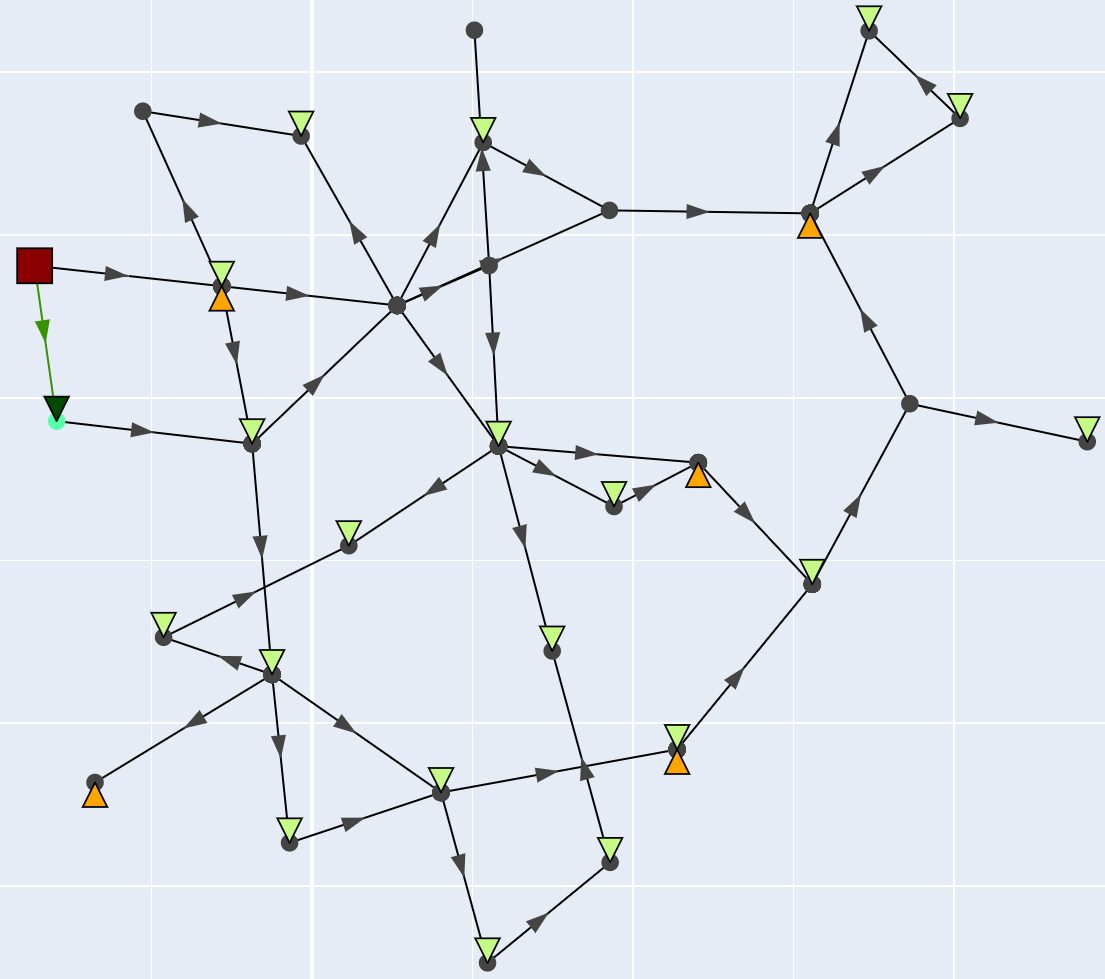
\includegraphics[width=\textwidth]{images/experiments/grids/30b_switched_off.png}
        \caption{Standard 30-bus scenario, with every component disconnected, except line 1 going to load 1}
        \label{fig:grid-30-off}
    \end{subfigure}
    \caption{Scenario showing the \ac{ppo} agent disconnecting most of the grid. The legend shown in \subref{fig:grid-14-off} applies to both subfigures}
    \label{fig:exp-grids-off}
\end{figure}

With the greedy agent the scores for $N-0$ overloads were also good, often reaching a score between the do-nothing and \ac{ppo} agents, however, it had problems with survival. Looking at the survival scores for each run, one can see them fluctuating between high and very low values. This is due to the exploitative nature of the greedy agent, only planning the current best step, but not looking ahead. This caused the agent to often do one substation-splitting action after another, changing the topology much more frequently than the \ac{ppo} agent. This caused the agent often to reach a non-converging state, where the simulation had to stop. 

An example of this behaviour can be observed in the standard, unmodified 30-bus scenario, shown in Figure \ref{fig:grid-30-greedy}. Here, the greedy agent repeatedly switches substations throughout the episode, in several instances even switching the same substation again in the very next timestep. As the external grid supplies by far the largest share of power to the 30-bus grid, these frequent and locally optimal, but globally uncoordinated, switching actions progressively worsen the loading of the transmission lines that carry power from the external grid to the highest-demand loads. This drives some line loadings above 130\% and causes bus voltages in the affected area to drop to as low as 15\% below the nominal level. As a result, the greedy agent survives only 26 of the 96 timesteps in this scenario. By contrast, the \ac{ppo} agent survives the full episode by resorting to its reward hacking strategy described above and shown in Figure \ref{fig:grid-30-off}, and the do-nothing agent also survives fully, though only after several lines are automatically put under maintenance due to excessive loading, cutting off the highest-demand load. Thus, both the \ac{ppo} and do-nothing agents stabilise the grid in this scenario only by sacrificing power delivery to parts of the grid, whereas the greedy agent fails to stabilise it at all through its uncoordinated switching behaviour.

\begin{figure}[htp]
    \centering
    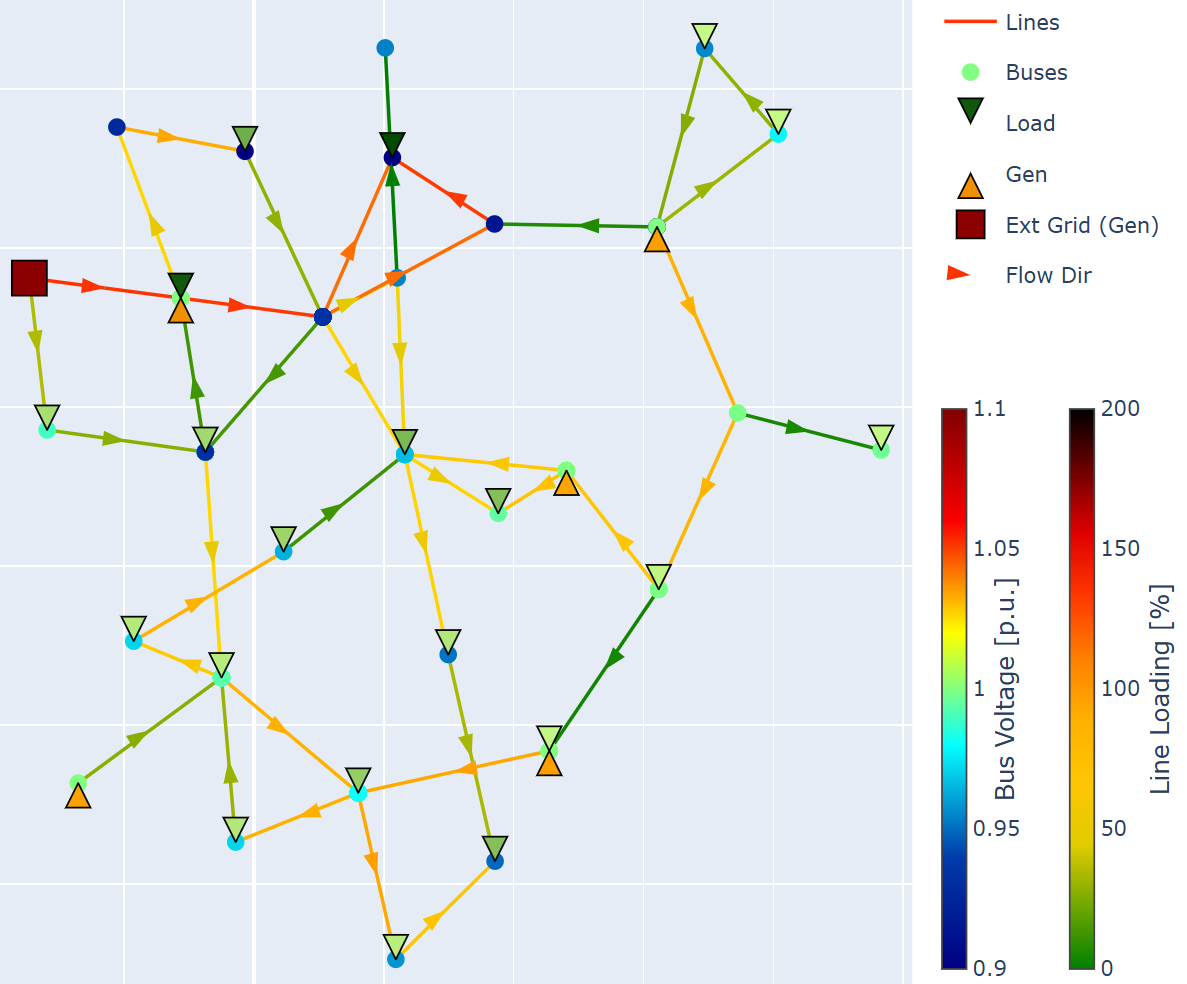
\includegraphics[width=0.57\textwidth]{images/experiments/grids/30b_original_greedy.png}
    \caption{Standard 30-bus scenario using the greedy agent, showing the last timestep before non-convergence was reached}
    \label{fig:grid-30-greedy} 
\end{figure}

In the overload mitigation category the do-nothing agent performed often worse than the other agents, due to not handling them at all. However, the survival score was almost as high as the one of the \ac{ppo} agent, which means that the experiments were not challenging enough, when it came to the survival category. Inaction was sufficient to avoid non-convergence for 70\% of the episode's timestep, on average.

For the voltage violation mitigation no agent had the goal to reduce them. This can be seen in Figure \ref{fig:metric-scores-voltage-violation} and in Table \ref{tab:agent_comparison}, as the average metric scores and category score for this aspect are much lower than the other metrics and categories. However, the \ac{ppo} agent had the highest scores, due to its strategy in some scenarios of disconnecting most of the power grid. 

When it comes to the cost category, it comes as no surprise, that the do-nothing has perfect scores for the metrics of substation changes and timesteps without actions. However, it is interesting that the \ac{ppo} agent learned to reduce the substation changes, while the greedy agent switches very frequently. While in some scenarios the \ac{ppo} agent only does one or two actions in total, the greedy agent often chooses different actions in each timestep. When it comes to load shedding, the \ac{ppo} agent performs very badly compared to the other agents. This is again due to its trained policy, which in many cases just delivers power to only one load close to the external grid, while not providing any power to the rest. 

\subsection{Influence of Grid Size}\label{ssec:influence-grid-size}
This subsection investigates the extent to which the size of the underlying power grid topology influences the benchmark scores, regardless of the specific grid modification applied. As the 14-bus and 30-bus grids differ substantially in terms of the number of components and electrical parameters, comparing their category scores directly may reveal systemic effects rooted in the grid structure itself rather than in the strategies employed by the agents.

As seen in Figure \ref{fig:exp-heatmap} and \ref{fig:bus-scores}, the category scores in the 14-bus power grid look different from the scores in the 30-bus grid. The 30-bus grid overall has higher scores, especially in survival and voltage violation mitigation. However, most of the scenarios that were compared, covered different grid modifications, making a direct comparison over all scenarios difficult. In general, each grid modification has much higher impact on the smaller grid, as the percentage of modified components is higher than in the bigger grid. If there are only three generators and eleven loads (see Figure \ref{fig:grid-14}), modifying one of them makes a significantly higher change, than changing one load out of twenty or putting one generator from five in maintenance.

Another difference that one can notice in all scenarios, is that the overload mitigation scores are lower in the 30-bus grid. When looking at the \textit{max\_i\_ka} values, it is clear why this happens. As explained in Section \ref{ssec:implementation-grid-mod}, \textit{max\_i\_ka} in pandapower defines the maximum allowed current (in kiloamperes), that can pass a transmission line or transformer. These values are at least 80 times higher in the 14-bus grid, than in the 30-bus grid. This extreme difference makes the lines in the 30-bus grid scenarios overload much faster, while they do not overload at all in the 14-bus grid. As the current can flow completely freely, this makes the 14-bus grid scenarios have other problems like power losses (regarding equation \eqref{eq:heat_power_dc}) and issues with nominal voltage levels (regarding equation \eqref{eq:high_voltage_low_current}). 

\subsection{Influence of Modifications}\label{ssec:influence-modification}
This subsection analyses the various grid modifications introduced in Section \ref{ssec:implementation-grid-mod} and their impact on the difficulty of a scenario. As the do-nothing agent does not perform any corrective actions, its scores can be used to isolate the impact of each modification on the power grid without the influence of an agent's strategy. The examination includes the effects of load and generator scaling, generator maintenance and line capacity scaling and maintenance.

\subsubsection{Load Scaling}
When looking at Figure \ref{fig:tot-score-diverse}, the load scaling in the 14-bus grid had the biggest impact. As seen in \ref{fig:scenario-scores-14b-up-ld0}, one of the three runs did not converge for any iteration and the second run got low survival scores overall. Also voltage violation mitigation has very low scores in this scenario, as shown in Figure \ref{fig:grid-14-load-inc} with the buses often being around 10\% over the nominal voltage level (visible in the colour scale in red; the darker the red, the higher the level). 

\begin{figure}[htp]
    \centering
    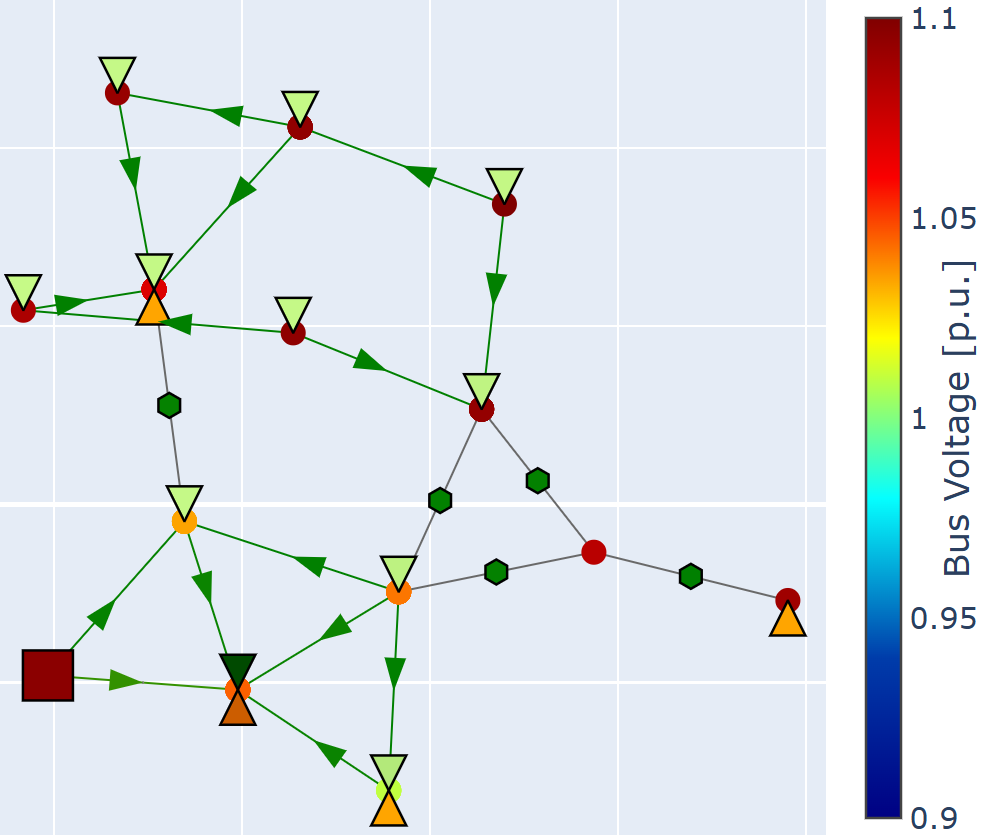
\includegraphics[width=0.5\textwidth]{images/experiments/grids/14b_load_inc.png}
    \caption{Bus voltages mostly above nominal level for the do-nothing agent in the 14-bus scenario with increased consumption at load 0}
    \label{fig:grid-14-load-inc} 
\end{figure}

For the 30-bus grids the upscaled load consumption in single loads caused the lines around the load always to be put into maintenance, due to the high line loadings. Figure \ref{fig:grid-30-load-inc} shows it for one run of the scaling of load 5, however, the results were the same in the other runs and with load 11 too. Always the lines connected to, or close to the scaled load reached overloadings. This made the scaled loads get no power at all, leading to poor scores in the costs and overload mitigation category, as Figure \ref{fig:scenario-scores-30b-up-ld5} and \ref{fig:scenario-scores-30b-up-ld11} show. In the 14-bus scenario with load scaling the lines did not have overloading issues. This is due to the \textit{max\_i\_ka} values in the transmission lines, explained in Section \ref{ssec:influence-grid-size}.

\begin{figure}[htp]
    \centering
    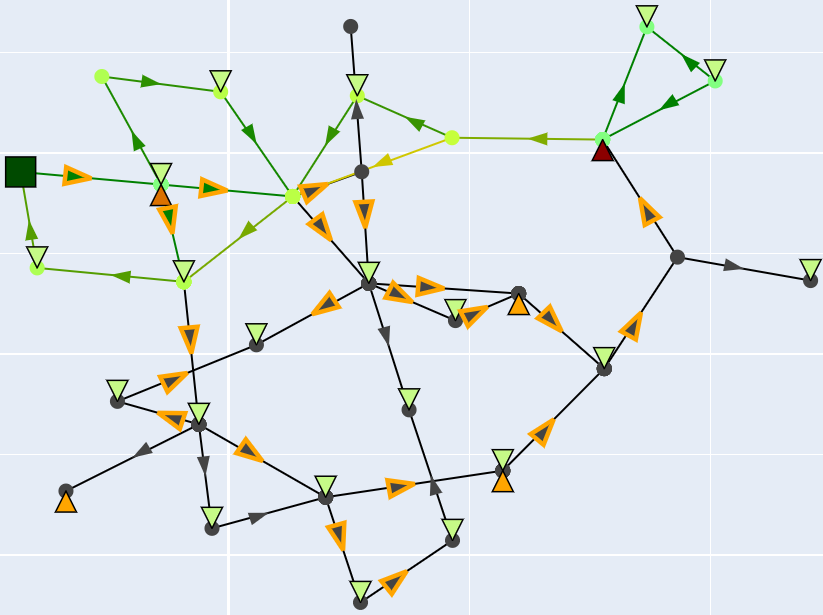
\includegraphics[width=0.54\textwidth]{images/experiments/grids/30b_load_inc.png}
    \caption{Lines in maintenance around load 5, for the do-nothing agent in the 30-bus scenario with increased consumption at load 5}
    \label{fig:grid-30-load-inc} 
\end{figure}

\subsubsection{Generator Scaling and Maintenance}
When it comes to increased power generation in the 14-bus scenario, it is visible, that it had an impact on the do-nothing and greedy agents' scores, achieving similar results to those of the load scaling scenario. When looking at Figure \ref{fig:scenario-scores-14b-up-gn0} it is clear, that both the do-nothing and the greedy agent struggled to maintain convergence and to lower the voltage violations. This is again due to the bus voltages, but contrary to the increased load, increasing the generation lowered the bus voltages. This is shown in Figure \ref{fig:grid-14-gen-inc}, where most buses are 10\% or more below the nominal voltage level (visible in the colour scale in blue; the darker the blue, the lower the level). 

\begin{figure}[htp] 
    \centering
    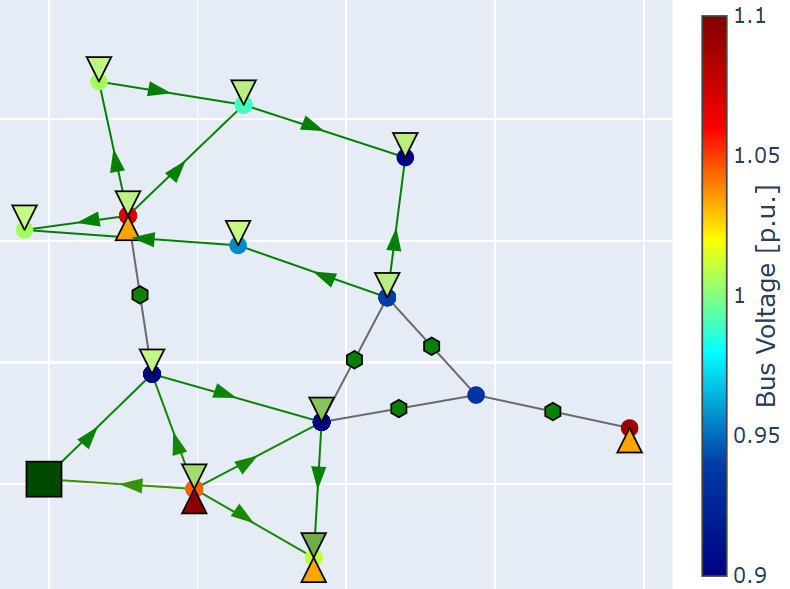
\includegraphics[width=0.53\textwidth]{images/experiments/grids/14b_gen_inc.png}
    \caption{Bus voltages mostly below nominal level for the do-nothing agent in the 14-bus scenario with increased production at generator 0}
    \label{fig:grid-14-gen-inc} 
\end{figure}

When it comes to the generator maintenance, that was applied in one of the 30-bus scenarios, the results are nearly identical to the normal 30-bus scenario. When looking at Figure \ref{fig:scenario-scores-30b-orig} and \ref{fig:scenario-scores-30b-mt-gn}, the scores are almost the same for each agent and category. Even when looking at the replay data, presented in Section \ref{ssec:replay-data}, the graphs of both scenarios look identical. The only difference is, that the external grid has to be used much more in the case of the generator maintenance, to make up for the missing power generation from the generator that is under maintenance. Other than that the same three lines overload and the rest of the grid runs relatively stable, making the do-nothing agent never reach a non-converging state. 

\subsubsection{Line Capacity Scaling and Maintenance}
For the grid modification of the line capacity scaling and line maintenance, the results behave very similarly in both modifications. For the do-nothing the same scores can be measured in all categories, as seen in Figure \ref{fig:scenario-scores-30b-mt-ln} and \ref{fig:scenario-scores-rc}. Due to the changes in the edges of the power grid, the grid goes into a complete shutdown at the 26th timestep in both scenarios. In both of them the shutdown is caused by a chain reaction, where multiple transmission lines reach an overloading over 150\% in the 25th step, causing them to be put under maintenance in the 26th timestep. After this step, all the lines connected to the external grid are under maintenance, removing a power source delivering around 250 MW of energy. Figure \ref{fig:grid-30-line-rc} demonstrates the 25th, showing the overloaded lines in a red to black colour, and 26th step, with overloaded lines marked with an orange arrow. The lines that are already overloaded in the 25th step are the ones that have been reduced in line capacity and thus overloaded in the first 20 steps. Making the grid completely powerless has a positive effect on the survival score, as when there is no power, the states always converge. The overload mitigation scores, however, are very low in these scenarios, due to constant overloadings.

\begin{figure}[htp]
    \centering
    \begin{subfigure}[b]{0.48\textwidth}
        \centering
        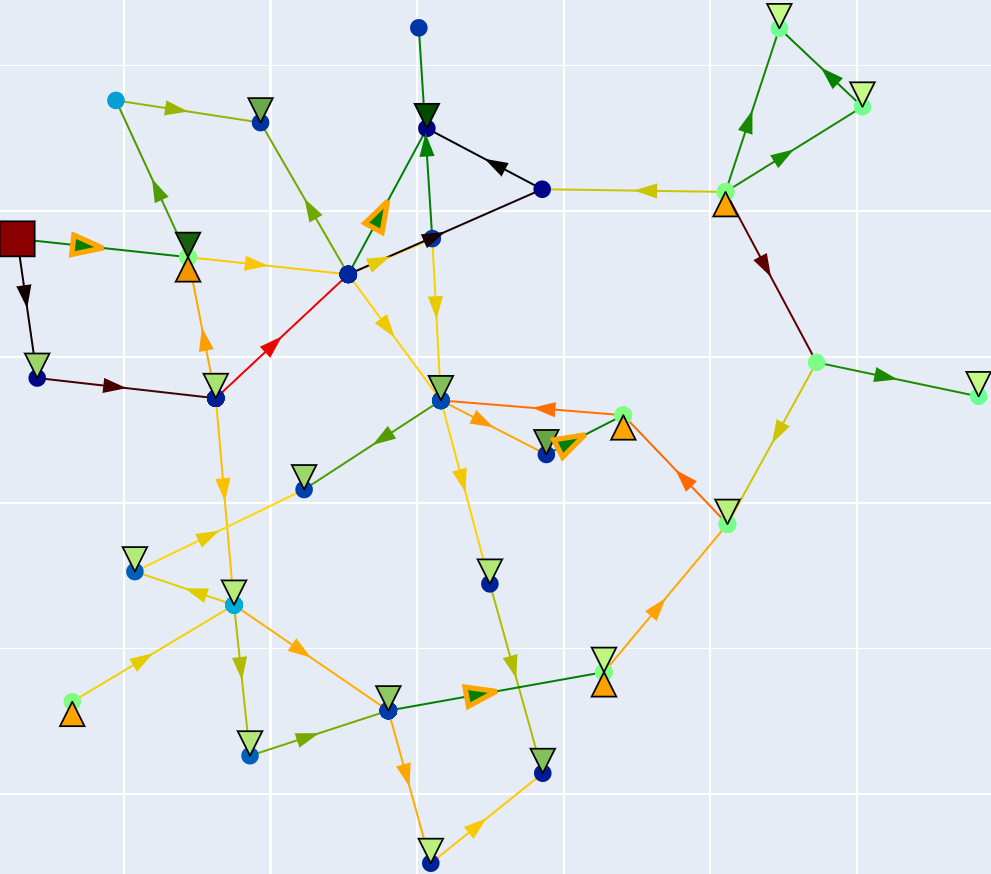
\includegraphics[width=\textwidth]{images/experiments/grids/30b_line_event_bf.png}
        \caption{25th timestep}
        \label{fig:grid-30-line-rc-bf}
    \end{subfigure}
    \hfill
    \begin{subfigure}[b]{0.48\textwidth}
        \centering
        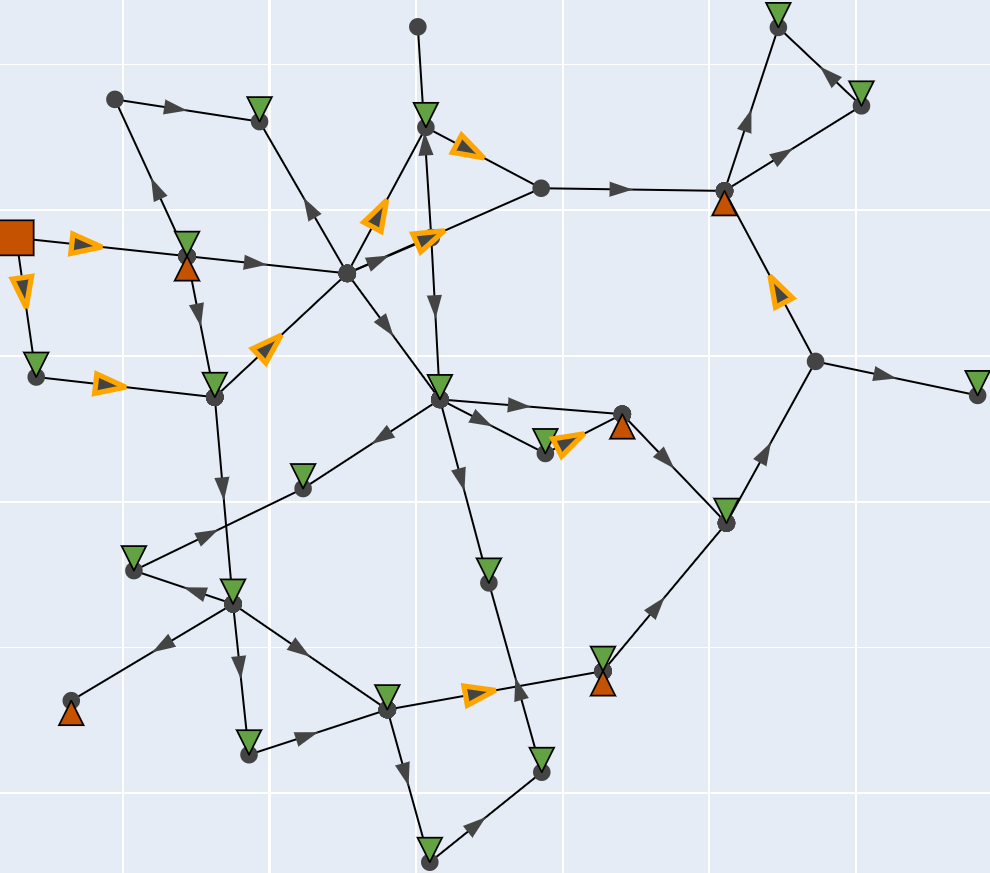
\includegraphics[width=\textwidth]{images/experiments/grids/30b_line_event_af.png}
        \caption{26th timestep}
        \label{fig:grid-30-line-rc-af}
    \end{subfigure}
    \caption{Complete powerless grid for the do-nothing agent in the 30-bus scenario with reduced line capacity}
    \label{fig:grid-30-line-rc}
\end{figure}


\subsection{Behaviour Under Increasing Stress}\label{ssec:behaviour-stress}
This subsection examines the results of the three stress tests conducted in the experiments, in which the generator, load and line capacity modifications are scaled up over multiple levels, to assess how the agents behave when scenarios diverge further from the nominal operating point. Comparing the category scores across these increasing scaling levels allows conclusions to be drawn about the robustness of each agent's strategy.

\subsubsection{Generator Stress Test}
For the generator stress test the do-nothing and greedy agents behaved as expected in Section \ref{ssec:exp-expectation}, as Figure \ref{fig:tot-score-gen-stress} shows. Both agents decline in performance over each increased level of difficulty. For the \ac{ppo} agent however, it is interesting to see, that it increased in scoring for the second scaling of the generator. In the second trial of this stress test, the agent reached perfect survival scores, while it achieved worse scores in the first scaling. When looking at Table \ref{tab:training-results} one can see, that the agent obtained more than double of the cumulative reward for the best training iteration for the second scaling compared to the first, lower scaling. Thus it was trained much better in $N-0$ overloads and grid convergence, and knew better actions. In the highest scaling it received the lowest cumulative reward over all trained scenarios, which explains the bad performance in the scenario. However, the third level of scaling is impossible to stabilise and get a score higher than zero, as it is already too unstable in the first profile step.  

\subsubsection{Load Stress Test}
The load stress test behaves as expected for all three agents, as Figure \ref{fig:tot-score-load-stress} demonstrates. However, the decline of the \ac{ppo} agent is worth noting, as it does very steeply between the first and second scaling, but not much for the last scaling. Even looking at the individual runs in Figure \ref{fig:scenario-scores-14b-up-ld0} and \ref{fig:scenario-scores-14b-up-ld0-high}, both scaling had similar category scores. This is not represented in the training values, as the second scaling had more than double of the cumulative reward compared to the third scaling. When looking at the actions in both scaling levels, the agent is always doing just one splitting action in the beginning and then no or just one action through the rest of the episode. With this it almost behaves like a do-nothing agent, not interacting much with the grid. With more tuning and training and a better reward function the agent could find better actions to interact with the grid.

\subsubsection{Line Capacity Stress Test}
The line capacity test resulted unexpectedly compared to the expectations formulated in Section \ref{ssec:exp-expectation}. The agents achieved almost constantly the same scores over each scaling, as Figure \ref{fig:tot-score-line-cap-stress} reveals. The reason for the same scores, is that the runs of each scaling behave exactly the same. As explained in Section \ref{ssec:influence-modification}, the second level of line capacity reduction made the grid turn into a powerless state in the 26th step. This event happens in the same way and at the same timestep for the other scaling of line capacity. For this reason the scores are all high, even in the highest scaling. With the grid being out of power, the grid stability can not become worse.

\subsection{Case Studies - Do-nothing vs. PPO}\label{ssec:case-studies}
In most scenarios of the experiments the \ac{ppo} agent achieved a higher or equal survival score than the do-nothing agent. However, there were a few cases, where the do-nothing agent beat the \ac{ppo} agent in convergence, even though the \ac{ppo} was trained to avoid it. In this section, three case studies are analysed more in depth, each of them focussing on one run of a specific scenario. In the first case study, the run at index 21120 (day 220) of the unmodified 14-bus grid is looked at. Here the do-nothing agent slightly outperformed the \ac{ppo} agent in the survival score, maintaining convergence a couple of timesteps longer. In the second case study, the second run at index 18240 (day 190) of the lowest generator stress test scenario is observed. This has the highest difference in grid convergence, as the do-nothing survived the full episode, while the \ac{ppo} agent only survived around 30\% of it. The final study looks at an opposite case. It compares the next level of the generator stress test, by looking at the same index as in the second case study. Here, even though it is the same profile day as in the second study with just more generator scaling, the scores in survival between the do-nothing and \ac{ppo} agents are swapped, with the \ac{ppo} agent clearing the episode while maintaining convergence.  

\subsubsection{Initial Observations} 
Firstly, for all the case studies, the actions are replayed, using the replay data presented in Section \ref{ssec:replay-data}. In general it stands out that the \ac{ppo} agent does just one or two actions directly in the first steps, and then it chooses no action, that changes the power grid. In Figure \ref{fig:grids-case-study}, one can see the obtained partial graphs of the grid, after the \ac{ppo} agent's actions have been implemented. For the first and second study, the agent does only one action, on one of the substations connected to one of the five transformers of the 14-bus grid. This does not seem to make a big difference, as the power grid's power flow just slightly changed, but all components still have paths between each other. In the third case study the agent splits the two substations, that are connected with a transmission line with the external grid, shutting off the rest of the grid and only providing power to the first load. The exact outcome is shown in Figure \ref{fig:grid-14-off}, which has been explained previously as being one of the agent's faulty strategy. Comparing this scenario to the others, it explains how the agent maintained convergence much longer in this scenario, compared to the other scenarios, where the agent did not follow this strategy. 

For the first study, the do-nothing performs a few steps more, than the \ac{ppo} agent. The action chosen by the \ac{ppo} probably brought a slight disadvantage to the agent, making it slightly less stable, in an already unstable grid, where inaction brings a quick failure of the grid. For the second study the do-nothing agent does not reach any non-converging grid states and finishes the whole episode, unlike the third study case, where the simulation ends after roughly a third of the episode. The changes in performance between the two cases is due to the increase of power production of generator 0. 

\subsubsection{Cross-Case Diagnostics} 
Now having compared each study, by only looking at the agents separately, a closer look at the two agents' performance is needed. For the 14-bus, as already discovered in \ref{ssec:influence-modification}, the lines do not have many issues with getting overloaded, thus a lot of current can pass through them. When performing a more detailed diagnosis of the simulations using pandapower's diagnostics functionality, warnings were issued for high \textit{vk\_percent} values (known as short-circuit voltage \cite{pandapower_docs} or percentage impedance \cite{impedance_percentage}) inside the transformers. This value controls how much a transformer resists the flow of power, in a similar way to resistance in an electrical circuit \cite{impedance_percentage}. In practice, this value is normally between 4\% and 15\%, and pandapower's diagnostic tool flags anything above 15\% as implausible \cite{pandapower_docs}. In the network model used for this thesis, all five transformers of the 14-bus grid had values above 1000\%. A higher value results in a greater voltage drop as more power flows through it \cite{impedance_percentage,transformer_impedance_regulation}. In these scenarios, the bus voltages around the transformers drop very low, sometimes even a voltage drop of up to 20\% compared to the nominal bus voltage. As explained in Section \ref{sssec:const_character_pg}, the voltages should remain within 10\% of the nominal value, to ensure a stable grid. These low values are explained, by the extreme \textit{vk\_percent} values in all of the transformers. These voltage drops make the grid extremely unstable. 

In the first two case studies, the \ac{ppo} agent chooses an action, which splits substations directly at one of the transformers. This causes changes in the current of the transformers, in an already highly unstable grid. For this reason, in the simulation of the \ac{ppo} agent, the bus voltages of the buses at the transformers are lower than the ones of the do-nothing agent. This makes the runs of the \ac{ppo} agent stop sooner than the ones of the do-nothing agent. On the third case study, however, the agent cuts off every part of the grid, except for the buses connected to the external grid and the load connected to it (as seen in Figure \ref{fig:grid-14-off}). This means, that the transformers are also not part of the grid, where power flows. This solves the instability caused by the transformers, making the \ac{ppo} agent go through the whole run, unlike the do-nothing agent that reaches non-convergence in the beginning of the run.


\subsection{Computational Performance}\label{ssec:computational-performance}
This subsection analyses the results of the performance test experiment presented in Section \ref{sec:experiment-results}, relating the measured runtime, CPU and memory usage back to the architectural differences between the greedy and \ac{ppo} agents discussed in Section \ref{ssec:custom-agent-setup}.

As expected, the \ac{ppo} agent is considerably faster than the greedy agent in both grid sizes. This is explained by the fundamental difference in how both agents select an action. While the greedy agent must simulate the resulting reward for every candidate switching action at every timestep, the trained policy of the \ac{ppo} agent maps a grid state directly to a single action. This difference becomes more obvious as the grid size increases. While the runtime per timestep of the \ac{ppo} agent remains almost constant between the 14-bus and 30-bus grid (1.32s vs. 1.44s), the runtime of the greedy agent more than doubles (3.98s vs. 8.47s), confirming the expectation formulated in Section \ref{ssec:exp-expectation} that the runtime advantage of the \ac{ppo} agent would be more significant in the larger grid, due to its larger action space.

The memory usage follows a similar pattern, with the \ac{ppo} agent using less than half the memory of the greedy agent in both grid sizes. This is likely because the greedy agent needs to keep multiple simulated copies of the grid state in memory simultaneously, one for each candidate action being evaluated, while the \ac{ppo} agent only performs a single forward pass through its policy network per timestep to decide an action.

The CPU usage, however, shows the opposite trend, with the \ac{ppo} agent consistently using more CPU than the greedy agent. This is presumably due to the batched matrix operations required for the neural network inference, which can utilise multiple CPU cores in parallel, whereas the sequential, one-by-one evaluation of candidate actions by the greedy agent does not fully utilise the available cores despite requiring a longer overall runtime. This illustrates, that the runtime advantage of the \ac{ppo} agent does not come without any computational trade-off, shifting resource demand from runtime and memory towards CPU utilisation. However, if the greedy agent were to parallelise its evaluation of candidate actions across more CPU cores, this would increase its CPU usage while also reducing its runtime per timestep. The user would then have to weigh the trade-off between a lower runtime and a lower CPU usage, depending on the computational resources available.



\subsection{Agent Behaviours and Profile}\label{ssec:agent-profiles}
Based on the observations from the previous subsections, this final subsection summarises the results to create a strengths and weaknesses profile for each of the three agents. This provides a concise summary of each agent's typical behaviour and demonstrates how the measured metrics and categories of \benchmark can be used to identify the capabilities and shortcomings of a power grid operation agent. Table \ref{tab:agent-profiles} summarises the discussed strengths and weaknesses of the three agents identified in the previous analysis. Each agent is then discussed in more detail below.

\begin{table}[htp]
    \centering
    \caption{Strengths and weaknesses of the evaluated agents}
    \label{tab:agent-profiles}
    \begin{tabularx}{\textwidth}{l X X}
        \toprule
        \textbf{Agent} & \textbf{Strengths} & \textbf{Weaknesses} \\
        \midrule
        Do-nothing &
        Perfect cost scores in action metrics (no actions at all); often high survival; no unintended load shedding &
        No overload or voltage violation mitigation; fails under increased stress \\
        \addlinespace
        Greedy &
        Decent $N-0$ overload mitigation, often between do-nothing and \ac{ppo}; reacts immediately to overloads &
        Highly unstable survival scores due to lack of lookahead; frequent substation switching (worst action metric scores); decline under stress; low computational efficiency \\
        \addlinespace
        \ac{ppo} &
        Highest scores in most metrics; learned to minimise substation changes; good in mitigating overloads and voltage violations; best convergence in several scenarios, even under stress; fast action computation &
        Reward hacking (disconnects most of the grid); lots of load-shedding; voltage improvements only a side effect of shutdown; can destabilise fragile grids via ill-timed splitting actions \\
        \bottomrule
    \end{tabularx}
\end{table}

\subsubsection{Do-nothing Agent}
\textbf{Strength Profile:} The do-nothing agent's main strength lies in its predictability and perfect cost scores, as it never performs any switching action (see Table \ref{tab:agent_comparison}). In scenarios not too far from the nominal operating point, inaction alone was sufficient to avoid non-convergence for a large share of the episode, as reflected in the survival scores of Figure \ref{fig:metric-scores-survival}. In individual case studies it even outperformed the trained \ac{ppo} agent in survival, most notably in the lowest generator stress test (Figure \ref{fig:tot-score-gen-stress}), where it completed the full episode while \ac{ppo} survived only about a third of it.

\textbf{Failure Profile:} Its main weakness lies in its design, which does not allow for any actions on the grid. Because of this it does not react to problems, resulting in low scores for overload and voltage violation mitigation across many scenarios. This is shown in the average metric scores in Figure \ref{fig:metric-scores-overload} and \ref{fig:metric-scores-voltage-violation} and also in the average scores shown in Table \ref{tab:agent_comparison}. As soon as a modification pushes the grid noticeably away from its nominal state, performance collapses, as shown in the load and generator stress tests (Figures \ref{fig:tot-score-load-stress} and \ref{fig:tot-score-gen-stress}).

\subsubsection{Greedy Agent}
\textbf{Strength Profile:} The greedy agent's strength is its fast, reactive overload mitigation, often scoring between the do-nothing and \ac{ppo} agents in the $N-0$ category, as seen in Figure \ref{fig:metric-scores-overload}. By always selecting the locally optimal action, it resolves immediate line overloads that the do-nothing agent does not handle.

\textbf{Failure Profile:} It is important to note that the scenario selection process described in Section \ref{ssec:experiment-scenarios} deliberately favoured profile days on which the greedy agent scored lower than the do-nothing agent. As a result, the failure profile presented here is likely more pronounced than it would be on an unfiltered, representative sample of grid conditions, and should be interpreted as an illustration of the greedy agent's worst-case behaviour rather than its typical performance across arbitrary scenarios. 
With this in mind, its short-sighted, purely exploitative strategy without lookahead is its main weakness. Performing one substation-splitting action after another causes frequent, large topology changes, leading to highly fluctuating grid stability and thus survival scores, as seen in Figure \ref{fig:metric-scores-survival}. This also leads to the worst scores in the cost category, when it comes to metrics that measure the frequency of actions. Furthermore, its performance deteriorates, when increasing the stress level, as Figure \ref{fig:tot-score-gen-stress} and \ref{fig:tot-score-load-stress} show, without any adaptive improvement. Additionally, it is not efficient in computational performance, needing a lot of time and memory in action decision. 

\subsubsection{PPO Agent}
\textbf{Strength Profile:} The \ac{ppo} agent achieved the highest overall scores across most of the metrics, particularly overload mitigation and survival, as Figure \ref{fig:metric-scores-overload} and \ref{fig:metric-scores-survival} and Table \ref{tab:agent_comparison} show. This confirms that its training objective of reducing $N-0$ overloads and avoiding non-convergence, was learned successfully. It also acts efficiently, often needing only one or two actions per episode, yielding better cost scores than the greedy agent. In several scenarios it kept the grid converging notably longer than the other two agents, for instance in the second generator stress test scaling, as shown in Figure \ref{fig:tot-score-gen-stress}. Additionally, in the computational efficiency test it achieved high scores, keeping the average runtime constant as grid size increases. 

\textbf{Failure Profile:} The agent's central weakness is in its policy, which uses a form of reward hacking. In multiple scenarios it learned to disconnect nearly the entire grid, supplying only a single load near the external grid to trivially avoid overloads and non-convergence, as illustrated in Figure \ref{fig:exp-grids-off}. This produces the worst load-shedding scores of all agents, as Figure \ref{fig:metric-scores-costs} shows. Moreover, its seemingly strong voltage-violation score, documented in Figure \ref{fig:metric-scores-voltage-violation}, is merely a side effect of powering down most of the grid rather than an active mitigation strategy. When it instead interacts through substation-splitting actions that do not disconnect most of the grid, as shown in Figure \ref{fig:grids-case-study}, it can occasionally worsen an already unstable state, causing earlier failure than a fully passive do-nothing agent. In certain situations involving increased stress, such as during the load stress test, the learned policy can also become almost completely passive, not improving the grid's state at all.
    \chapter{Discussion}\label{ch:discussion}
This chapter discusses the design, capabilities and limitations of \benchmark, building on the concept, implementation and experiments presented in the previous chapters. Section \ref{sec:discussion-benchmark-design} discusses key design decisions behind \benchmark, focusing on its hierarchical scoring system and its configurable components. Section \ref{sec:evaluation-benchmark-principles} evaluates \benchmark against the principles of a well-designed benchmark introduced in Section \ref{ssec:principles-benchmark}. Section \ref{sec:existing-benchmark-comparison} compares \benchmark to the related benchmarking tools discussed earlier in this thesis. Section \ref{sec:experiment-learnings} reflects on the key learnings drawn from the experiments conducted in Chapter \ref{ch:experiments}, regarding how \ac{rl} agents for power grid operation should be benchmarked in general. Finally, Section \ref{sec:discussion-limitations} discusses the limitations of this work.




\section{Discussion of Benchmark Design}\label{sec:discussion-benchmark-design}
\benchmark offers a customisable benchmark that allows users to create experiments by giving them a selection of scenarios, with each scenario offering a chosen power grid and profile from the IEEE test cases and SimBench. The grid modifications offer the possibility to modify the grid data to create more diverse scenarios. This customisability introduces several design decisions that are discussed in this section. First, the hierarchical scoring system is discussed, covering how the underlying metrics are used, how they are aggregated across multiple layers, and how the resulting scores are presented back to the user. Second, the configurable components of the benchmark are discussed, namely the scoring weights and the scenario selection, which together define the objective and quality of a given benchmark trial.

\subsection{Scoring System}
The scoring system used by \benchmark structures the evaluation of an agent's performance across multiple layers, ranging from individual grid metrics to a single, aggregated total score. This subsection discusses the design of this scoring system, covering how the underlying metrics are used and normalised, how the resulting scores are aggregated across the hierarchy, and how the different layers are presented back to the user for interpretation.

\subsubsection{Metrics Usage}
As demonstrated in Section \ref{sec:metrics-eval}, each experiment has a hierarchical scoring system. On the lowest layer, there are multiple grid metrics that are measured during a single run. Multiple metrics were chosen, as there is not one single metric that can provide all the information needed on the agent's performance. Each of them focusses on only one grid or operational feature, covering multiple features that are important in evaluation of an agent in power grid operation. While most features focus on grid stability, some focus on operational cost or computational efficiency. All of these categories are relevant in a strong performance in power grid operation, as managing a power grid must also remain under a specific budget limit, without causing costs to rise. Also, the computational efficiency is crucial in real-time power grid operation, when the agent needs to react and decide on the next actions quickly, or when the computational resources are limited.

Furthermore, the metrics are converted into a normalised score from 0 to 100 by using a linear function, relative to the worst and best reference values. The normalisation into 0 to 100 makes every metric comparable and simple to interpret, as the score values are in a percentage-based range. Additionally, the normalisation allows aggregation across the metrics, due to the same value range for each metric. 

\subsubsection{Score Aggregation}
The first aggregation happens with categories, which group the metrics and provide a summary of how well the agent performed for specific types of grid metrics in one run. Each category covers a crucial aspect of strong performance in power grid operation.

Each run then receives a weighted average score of the categories, which is then used to calculate the average scenario score. This provides another summarised feedback for the next two layers, run and scenario layers. Without needing to see all the measured metrics and their scores, it is possible to directly assess the performance of each run and scenario. Finally, the highest level of summary is the total score, which is calculated as the average of the scenario scores. This gives feedback for the overall performance, without showing any details about the exact metric, category or other scores. 

Each layer in this hierarchical scoring system has its importance. The higher layers summarise information to provide a simple comparison value for quick evaluation. The lower layers gather specific data points and create scores for them, thus having the most information about individual performances. The lower layers are crucial for analysing the agent's behaviour and finding patterns or problems.

\subsubsection{Result Presentation}
Building on the multiple aggregated scores across different layers of the hierarchical scoring system, \benchmark offers many ways to present the results of a benchmark trial. As shown in Section \ref{sec:result-format}, the result presentation ranges from statistics, plots, web UIs for analysis and comparison, and pages for replay of a run. These presentations again emphasise the premise that one single score is not sufficient for meaningful feedback. They showcase each scenario and run, creating different textual reports and visualisations for them. Additionally, the comparison views allow contrasting multiple agents directly against each other on the same scenario or category, making it easier to identify in which specific aspects one agent outperforms another, rather than relying on the total score alone. Furthermore, with the replay tool, the users can perform more thorough diagnostics of the agent's behaviour, or better understand its benchmark scoring by visually inspecting the exact grid state and action taken at each timestep of a run. This is particularly valuable for detecting behaviour that is not directly captured by the metrics themselves, such as the reward hacking behaviour discussed in Chapter \ref{ch:experiments}.


\subsection{Configurable Components}
Both the scoring weights and the scenarios are configurable components of the benchmark. They determine the objective and quality of the benchmark. This flexibility allows \benchmark to be tailored to different research questions and evaluation goals, ranging from safety-oriented to cost-oriented evaluations, but it also shifts the responsibility onto the user to configure these components in a meaningful way. The following two subsections discuss the weights and the scenario selection individually, highlighting how each shapes the outcome of a benchmark trial.

\subsubsection{Weights}
In the lower layer of the scoring system, the metrics and categories have configurable weights. The user sets these to emphasise or omit specific parts of the evaluation. This makes it possible for researchers to create benchmarks that are tailored to their objectives. They can create a safety-oriented, cost-oriented, or computational-efficiency-oriented benchmark or a mix of them, which creates different ranking possibilities. 

Another use-case is shown in Chapter \ref{ch:experiments}, with two benchmarks focussing on grid operation and computational-efficiency. In the computational performance category, the do-nothing agent outperforms other agents, as it is used as the ideal reference point for minimal calculation complexity and time. It would not make sense to compare this agent directly with the greedy or \ac{ppo} agent. Thus, the configurable weights are used to create multiple benchmarking trials, which each analyse different aspects in power grid operation and evaluate different agent types.

\subsubsection{Scenario Selection} 
Another configurable part of a benchmark is its evaluation trials. In \benchmark, they are called scenarios, each covering one power grid, profile, grid modifications and specific indices in the profile. Together with the weights, they form a specific benchmark. The weights and scenarios define the objective of the benchmark and what it should evaluate. However, the scenarios also set the complexity and quality of the evaluations. Depending on the chosen scenarios, the coverage and difficulty can differ. The objective of the user might be diverse scenario or stress condition testing, or the users want to research a specific type of power grid and choose only that type as scenario. 

The importance in the design of \benchmark is that multiple scenarios are run in one benchmark trial. This ensures that the agents are tested on a high coverage dataset, which reveals whether the agent has strengths or weaknesses for specific scenarios. With only a single scenario, it is not possible to conduct a thorough analysis of an agent's capabilities in power grids.

However, this configurability also makes the resulting benchmark quality dependent on the user. If the user chooses poor configurations, then the benchmark might produce misleading conclusions about the agent's performances. Therefore, the selection of scenarios needs to be implemented with an objective in mind, and this objective should be pursued through multiple scenarios that have a high coverage of the possible cases.





\section{Evaluation of Benchmark Principles}\label{sec:evaluation-benchmark-principles}
Having established the principles of a well-designed benchmark in Section \ref{ssec:principles-benchmark}, this section evaluates the benchmark presented in this work against these criteria. Each principle is discussed individually, considering both the aspects that were successfully addressed and those that were only partially fulfilled.

\paragraph{Definition of Objective.}
As for clear objectives, \benchmark offers the user many choices, which define the objectives of the evaluation. For example, the user must decide which metrics and categories are important for evaluation and which scenarios should be covered to benchmark the agents. The benchmark then focusses on these cases and evaluates only these settings. The metrics and categories chosen for the trials cover important parts of optimal grid operation, considering grid stability and cost factors. These aspects follow the broader research objective of improving agents for power grid operation. However, this flexibility also means that \benchmark does not enforce or suggest a specific objective by default. Users unfamiliar with power grid operation may struggle to select a meaningful combination of metrics, categories and scenarios, which could lead to an evaluation that does not reflect a clearly defined or well-motivated objective.

\paragraph{Reproducibility.}
For reproducibility, the benchmark does not use any seeds for evaluation because the internal benchmark processes always run deterministically. The benchmark always performs the same tasks for the same input scenarios. After the agent runs through the different trials and the actions are saved internally, the evaluation process is always identical when the same run values are loaded, and identical scores are calculated. However, this only guarantees the reproducibility of the internal benchmark processes, not the reproducibility of the agent's behaviour itself. If an agent uses a stochastic policy or otherwise non-deterministic decision-making process, its actions, and therefore its resulting scores, may differ between runs of the same scenario, even though the benchmark process itself is fully deterministic. 
Additionally, stochasticity can be introduced for learned agents during training. For example, this can be achieved through random weight initialisation or non-deterministic exploration. This means that even a deterministic evaluation policy may produce different results for instances of the same agent that have been trained in different ways.
This limitation is discussed further in Section \ref{sec:discussion-limitations}.

\paragraph{Comparability.}
As seen in the experiments in Chapter \ref{ch:experiments}, \benchmark offers a structured comparability between multiple agents. It not only shows the best overall agent, but also the strengths and weaknesses among other agents and between different trials. Thus, it does not simply answer the question of which agent is the best. Instead, it provides an analysis of different cases and metrics inside power grids and a ranking over these features. However, in case of the \ac{ppo} agent's reward hacking, shown in the experiments, this was not captured by the metric system. The replay function made it possible to see more information on each agent, but it is not something measurable or comparable with the other agents. It merely shows whether the agent chooses questionable actions that are not optimal in power grid operation. 

\paragraph{Transparency.}
Through this work, the documentation\footnote{\documentation} and the evaluation results being stored in a human-readable JSON format (as presented in Section \ref{sec:int-processes}), the results are interpretable for the user. With the further visualisation tools presented in Section \ref{sec:result-format}, the user gains even more insight into the agent's performance during the benchmark experiments.

\paragraph{Relevance.}
As explained in Section \ref{sec:implementation-scenarios}, the power grid data for grid topology and profiles is provided by IEEE test cases and SimBench data. Both sources offer realistic power grid data for benchmarking power grid systems and cover different types of power grids. However, as discussed in Section \ref{sec:exp-analysis-interpretation}, some of these test cases contain physically implausible parameter values, limiting how closely the benchmark reflects real-world grid behaviour in these cases.

\paragraph{Representativeness.}
The quality of the benchmarking solely depends on the settings and the diversity of scenarios chosen by the user. This determines the representativeness, depending on the coverage of evaluated edge cases. The more scenarios are selected, especially with different grid modifications, the better the coverage is. However, when working in teams or in a competition, a set of diverse scenarios with high coverage and specified evaluation criteria can be predefined, allowing multiple agents to be compared and enabling a diverse benchmark set for research on agent improvement.





\section{Existing Benchmark Comparison}\label{sec:existing-benchmark-comparison}
Earlier in this work, several existing benchmarking tools for \ac{rl} agents in power grid operation were introduced, namely PowerGym, \ac{l2rpn} and RL2Grid, and summarised in Table \ref{tab:power-grid-benchmarks}. This section revisits these benchmarks and compares them directly against \benchmark, highlighting differences in scoring design, scenario diversity, safety handling and result presentation.

\paragraph{PowerGym.}
As discussed in Section \ref{ssec:power-benchmark}, PowerGym offers a benchmark on Volt-Var control systems in distribution grids. It uses the IEEE test cases for each evaluation and makes these cases modifiable like in \benchmark. As the objective of this benchmark is narrower, it makes the final scoring easier to interpret. The flexibility of \benchmark enables a broader evaluation, but at the cost of requiring additional configuration choices that directly influence the final ranking. However, the benchmarking feedback is measured as the cumulative reward, while the reward is composed of multiple grid metrics. This is a structural difference from \benchmark, with the feedback of PowerGym being single-dimensional. The experiments in Chapter \ref{ch:experiments} showed how crucial it is to analyse agents at multiple levels of depth to pinpoint unexpected problems, even when the overall score appears strong. Evaluating additional independent metrics or diagnostic tools can expose such behaviour.

\paragraph{L2RPN.}
The \ac{l2rpn} challenge provided realistic power-grid scenarios, with hidden evaluation scenarios, which are executed on a central server. For each submitted agent, it computed a standardised competition score, which was used for a leaderboard. With \benchmark, there is no evaluation server or leaderboard, and the flexibility in configuration makes it possible for two research groups to select completely different evaluation bases. The scores created by both research groups would not be comparable between the groups, due to differences in scenarios or score composition. Furthermore, due to the number of participants in \ac{l2rpn}, its design received substantially more external validation compared to the newly presented benchmark of this work. Additionally, the scoring also has a structural difference. In \ac{l2rpn}, it is relative to the do-nothing agent as a baseline, while in this work the do-nothing agent is used more as a selection model for choosing the scenarios. It is only used in the computational performance as a scoring reference. The advantage of the \ac{l2rpn} scoring system is, that each scenario is scored similarly, no matter how complex and difficult it is. If in a scenario it is harder to solve grid stability, then the do-nothing agent would also perform worse and the evaluated agents require similar effort to achieve a score above 0, as with easier scenarios. In \benchmark, the scoring also depends on the scenario difficulty, as the experiments in Chapter \ref{ch:experiments} showed. When a scenario was impossible to operate, as the first iteration already reached non-convergence, then all the agents received the lowest score. However, the scoring in \ac{l2rpn} was not fully transparent. While \benchmark uses a linear scoring system with worst and best values, in \ac{l2rpn} it remains unclear exactly how values between the fixed score points of -100, 0, 80, and 100 are calculated. Furthermore, this score is again a cumulative score, focused on competitive ranking for the leaderboard. This takes information away from single runs and makes diagnostics impossible. Moreover, the evaluation in \ac{l2rpn} is conducted only on one core grid environment, instead of offering a variety of different grids to test. Even though the experiments shown in Chapter \ref{ch:experiments} only covered two grids, \benchmark offers other grids from the IEEE test cases and SimBench data.

\paragraph{RL2Grid.}
RL2Grid builds on \ac{l2rpn} and comes closest to the benchmark of this work. It improves \ac{l2rpn} by adding more grid environments using Grid2Op systems, synthetic ChroniX2Grid profiles, expert-informed heuristics that emulate human operator behaviour and \ac{cmdp}-based safety constraints. The safety constraints offer the strongest advantage over \benchmark, as it improves safety by avoiding load shedding and islanding and thermal-limit violations. While load shedding and thermal limits are covered in the metrics of this work, load islanding is not part of the evaluation. The case study in Section \ref{ssec:case-studies} demonstrates that safety-critical behaviour may not always be adequately represented by metrics, thus leading the \ac{ppo} agent to choose actions that caused load shedding and islanding. This is avoidable using a constraint system, just like in RL2Grid. Additionally, RL2Grid includes an expert-informed heuristic, which suppresses unnecessary actions when the grid is already stable enough, so that the heuristic can incrementally restore the original topology. This covers a stronger integration of \ac{tso} operational knowledge into the benchmark process, which \benchmark does not possess. This is also an advantage for the agent's training and testing, as it reduces the task to challenging parts, where the agent needs to stabilise the grid. In terms of grid diversity, both tools offer a solid amount of usable scenario data, with the Grid2Op and ChroniX2Grid data in RL2Grid and the IEEE test cases and SimBench in \benchmark. Additionally, some of RL2Grid's larger grids include battery storage units, a feature not currently modelled in \benchmark's grid data.
As for the evaluation metrics, \benchmark offers more dimensions compared to the survival metrics and the three operational metrics (line margin, overloads and topology changes) in RL2Grid. This makes comparison over different agent strategies more limited for RL2Grid. Furthermore, the category of computational performance is not included in RL2Grid. This category is crucial in real-time control, as a policy that cannot meet operational timing constraints may be practically unusable. Another advantage of the benchmark in this work is the different formats in which results can be displayed. \benchmark offers a result-exploration layer, which enables in-depth analysis of the results and makes it easier to pinpoint outliers. The replay functionality offers fault detection for the agent's scoring by displaying its actions. Another disadvantage of RL2Grid is its use of random starting points or random line disconnections, reducing exact reproducibility, while \benchmark uses fixed configurations for the whole trial.





\section{Learnings from the Experiments}\label{sec:experiment-learnings}
The experiments conducted in Chapter \ref{ch:experiments} did not only serve to demonstrate the capabilities of \benchmark, but also provided broader insights into how \ac{rl} agents for power grid operation should be benchmarked in general. This section summarises four such learnings, regarding agent comparison, score aggregation, the role of baseline agents, and the influence of scenario configuration on the resulting conclusions.

\paragraph{Universally Strongest Agent.}
When comparing the three agents in the experiments, the results showed, that there is no single agent, that was universally strongest. Some agents excel in some scenarios, but fail in others. This was visible with the \ac{ppo} and do-nothing agents, that often competed for first place in the scenario scores. In some runs one agent was stronger, in others the other was stronger. It was never just one agent beating all of them. Agent quality is scenario-dependent and a benchmark has to illustrate this, to show strengths and weaknesses.

\paragraph{Score Aggregation Conceals Information.}
When looking at the \ac{ppo} agent, it overall achieved the best scores over the whole experiment. However, when taking a closer look, the agent seemed to have found a way to achieve high rewards, but still operate in unsuitable ways for power grid operation. This was discussed in Chapter \ref{ch:experiments} as a case of reward hacking, which made the \ac{ppo} agent achieve high scores but exhibit low usability in real-world operations. In summary, a high benchmark performance does not automatically imply operationally desirable behaviour. The actions of each agent should be analysed in depth, before deciding how well an agent performs.

\paragraph{Baselines Provide Context.}
Another finding from the experiments was the usefulness of the baseline agents. Even though the two baseline agents used simpler strategies, compared to the trained \ac{ppo} agent, they were still useful for the experiment interpretations. For example, in some scenarios the do-nothing agent survived surprisingly long, as shown in Section \ref{ssec:case-studies}. In contrast, the greedy agent acts as the opposite of the do-nothing agent, by intervening frequently without any long-term robustness in many scenarios. Both baselines provide information in each scenario, not only for ranking against other agents, but also for interpreting the scenario's difficulty. The worse the baselines perform, the harder it is for other, more complex agents to maintain grid stability.

\paragraph{Configured Scenarios Affect Conclusions.}
As discussed in Section \ref{sec:discussion-benchmark-design}, the scenarios chosen by the user strongly affect the conclusions of the benchmarking. Each of the grid modification experiments in Chapter \ref{ch:experiments} demonstrates that the outcomes differ. When using only a part of these experiments, the conclusions are more limited and result in a different scoring and thus ranking of each agent. Through the experiments, it is clear that one scenario or just one run is not sufficient for a deep understanding of each agent's performance. A diverse set of scenarios is essential for a stronger benchmark quality and a better analysis of each agent. 




\section{Limitations}\label{sec:discussion-limitations}
While \benchmark addresses the research question posed in this thesis, the experiments conducted with it also revealed several limitations that should be considered when interpreting the presented results. This section discusses five such limitations, concerning the selection of agents and grids used in the experiments, the quality of the underlying grid data, the handling of stochastic agent behaviour, and the computational evaluation environment.

\paragraph{Limited Agent Selection.}
During the experiments, only three agents were evaluated. Additionally, only one of these agents has a learned \ac{rl} architecture. For this reason, this work did not fully validate \benchmark across different \ac{rl} architectures, such as those discussed in Section \ref{ssec:example-agents}. A broader comparison across value-based, policy-based and hybrid architectures, as discussed in Section \ref{ssec:future-agents}, would be necessary to assess whether the observed differences in benchmark scores generalise across agent types.

\paragraph{Limited Grid Selection.}
Another limitation in the experiments is the lack of variety in different grid topologies. Only two IEEE test cases were evaluated, but the benchmark supports more grids. The benchmark focussed more on grid modification and finding challenging scenarios, but it lacks testing on larger transmission grids or real-world grids. This limits the ability to draw conclusions about how \benchmark scales to larger, more interconnected grids, where topology actions may have different effects on grid stability.

\paragraph{Grid Quality.}
As discussed in Section \ref{sec:exp-analysis-interpretation}, the 14-bus grid from the experiments has some physically implausible values for the grid edges, such as the \textit{vk\_percent} values in the transformers or the \textit{max\_i\_ka} values in the transmission lines. For this reason, some observed instability may originate partly from the grid model rather than the agent performance. This limits the interpretation of some experimental results. This expands the lesson from Sections \ref{sec:discussion-benchmark-design}, \ref{sec:evaluation-benchmark-principles} and \ref{sec:experiment-learnings} about the benchmark quality. The benchmark quality is bounded by the selection of the scenarios \textbf{and} the quality of the scenario model.

\paragraph{Stochastic Evaluation.}
The benchmark scenarios and scoring procedure are deterministic for a fixed configuration. However, individual agents may introduce stochastic action selection, depending on their implementation. For this reason, running each of the scenario runs only once would not be practical in case of stochastic decisions inside the evaluated agent. Instead, each run needs to be repeated multiple times to calculate an average score for each metric score of a run. Furthermore, the user should be able to set one or multiple seeds, to have a fixed testing environment for these types of agents. This seed needs to be used by the agent, so that the stochastic decision-making is reproducible. In addition to stochasticity at evaluation time, learned agents may also be affected by stochasticity introduced during training, such as random parameter initialisation or exploration noise. Consequently, two agents trained using the same algorithm and hyperparameters but different training seeds may produce different policies and thus achieve different benchmark scores. Therefore, a thorough evaluation should consider training multiple instances of the same agent with different training seeds to determine how much of the measured performance is attributable to the algorithm itself rather than a specific training run.

\paragraph{Computational Benchmark Environment.}
As the experiment testing computational efficiency was only run on one machine, the values are hardware-specific. To produce a stronger and more general evaluation of the two tested agents, it is necessary to test the computational efficiency on multiple machines. Additionally, computational performance measurements are inherently variable as they can be affected by external factors, such as background processes or system load, at the time of measurement. Therefore, a single run is not sufficient to obtain a reliable estimate, similar to the handling of stochastic agent behaviour discussed above. Multiple repetitions of each measurement are necessary to obtain stable and representative values. Furthermore, the current evaluation only measures an agent's overall inference time, without profiling or tracing its internal computations. Consequently, it is impossible to determine why one agent is faster or slower than another or which parts of its decision-making process are computationally expensive. Agents can be implemented with varying degrees of efficiency, for example through optimised code or better use of hardware acceleration, but this simple timing measurement alone cannot capture or distinguish such implementation-specific differences. Future work could address this by integrating dedicated profiling tools, allowing a more detailed breakdown of an agent's computation time across its decision-making pipeline.
    \chapter{Conclusion}\label{ch:conclusion}
This thesis addressed the challenge of evaluating and comparing \ac{rl} agents for power grid operation. Motivated by the increasing complexity of modern power grids and the growing interest in using \ac{rl} agents to support grid operators, the research question was formulated: \begin{displayquote}
How can a benchmarking tool be designed to quantitatively and qualitatively evaluate and compare agents for power grid operation, providing both an overall performance score and detailed feedback on their strengths and weaknesses across different operating scenarios?
\end{displayquote}
To answer this question, the benchmark \benchmark was designed, implemented and evaluated through a series of experiments, presented in Chapters \ref{ch:methodology}, \ref{ch:implementation} and \ref{ch:experiments}. This chapter concludes the thesis. Section \ref{sec:contributions-findings} summarises the main contributions of \benchmark and the key findings of the conducted experiments, relating them back to the research question. Section \ref{sec:future-work} then outlines possible directions for future work that emerged during the development and evaluation of the benchmark.




\section{Contributions and Findings}\label{sec:contributions-findings}
This section summarises the main contributions of this thesis and relates them back to the research question. Section \ref{ssec:contribution-benchmark} presents the contributions made through the design and implementation of \benchmark, outlining how its features address the research question from a design perspective. Section \ref{ssec:contribution-experiments} summarises the key findings of the experiments conducted in Chapter \ref{ch:experiments}, validating the benchmark's capabilities empirically. Finally, Section \ref{ssec:contribution-takeaway} condenses the most important insight of this thesis into a single, concise takeaway.

\subsection{Benchmark}\label{ssec:contribution-benchmark}
The developed benchmark \benchmark, presented in this work, is a configurable metrics- and scenario-based benchmark for agents working in power grid operation on the transmission grid. Each scenario specifies one power grid, provided by the IEEE test cases or the SimBench dataset, and one profile from the SimBench dataset, where specific indices from the profile are chosen for evaluation. The grid of a scenario is modifiable, with different possible grid modifications that are configurable by the user. Grid modifications create extreme scenarios with imbalanced grid components. This includes increased generation or consumption in one generator or load, maintenance events that make grid components unusable for the scenario, or capacity scaling, which limits the possible usage of lines or transformers. 

For benchmarking agents, \benchmark offers different options. Either one of two baseline agents can be chosen, or a custom agent created by the user. To use a custom agent, two blueprint classes exist, from which the custom agent inherits. The \texttt{BenchAgent} defines the necessary interfaces that \benchmark needs to interact with a custom agent, such as agent setup, training and action selection. The \texttt{RayAgent} is a subclass of the \texttt{BenchAgent} and offers an interface for agents that use the Ray framework for building their \ac{rl} architecture. It simplifies agent definition for Ray agents, as only the agent initialisation needs to be implemented. Furthermore, the \texttt{BaseTuner} exists for hyperparameter tuning of an agent before training. This class also has a subclass, the \texttt{OptunaTuner}, which simplifies making hyperparameter tuners for custom agents using the Optuna optimisation framework. For each scenario, a custom agent can be tuned using a customised tuning class, and is then trained on the scenario using user-specified training indices from the scenario profile. After training, the evaluation indices from the scenario profile are each executed individually to evaluate the agent.

The evaluation of each run in a scenario is built on a multi-dimensional metric framework. It measures multiple grid features, and converts them into a normalised score, each within the same range of 0 to 100. To summarise all the gathered scores, the scores are aggregated and form a hierarchical scoring system. Each layer of the scoring system summarises the performance of the grouped scores underlying the layer. The category score summarises multiple metric scores, using configurable weights for each metric. The run score summarises multiple category scores, with each category containing a configurable weight as well. Finally, the scenario score summarises the run scores, and the total score summarises all scenario scores, on average. For fixed run data and deterministic agent behaviour, the benchmark evaluation and scoring procedure is reproducible. Full experimental reproducibility additionally depends on controlling the agent's stochasticity and random seeds.

The gathered results can be presented using different included tools. These create statistics, visualisations with plots and web apps, and comparisons between agents. With the help of these, the benchmark results are summarised and presented in a way that the user can analyse every layer of the hierarchical scoring system and how well the agent performed for specific scenarios or metrics. In addition to these tools, the replay tool creates a visualisation from the run data gathered during the scenario execution. The replay tool offers an analysis of the actions taken by an agent and how stable the grid was in each timestep. This provides another analytical layer to the benchmark, where users can understand the agent's behaviour and scoring.

The multi-dimensional metrics and hierarchical scoring system make this benchmark different from the past works presented in Section \ref{sec:rw-benchmarking}. Furthermore, it has more diagnostic tools built in, which make a stronger analysis into the agent's performance possible. With regard to the research question, the benchmark presented in this work addresses both its quantitative and qualitative aspects. It provides a quantitative evaluation using normalised metric scoring, offering a variety of metrics to measure and evaluate different grid features. These metric scores are then summarised using a hierarchical aggregation system, which gives an overall performance score. Furthermore, it delivers a qualitative evaluation by offering visual and textual reporting formats and a replay tool, which reveal how an agent behaves, not just how well it scores. The output saved by the benchmark does not just store the aggregated total score. It also provides information on each layer of the benchmark, from specific metric scores in single runs, up to aggregated scenario scores. Additionally, the reporting tools demonstrate the strengths and weaknesses that each agent has for specific metrics, categories or operating scenarios. The scenario tuple design enables diverse, reproducible, and configurable test conditions. 


\subsection{Experiments}\label{ssec:contribution-experiments}
Another important part of this work is the experiments presented in Chapter \ref{ch:experiments}. The experiments tested \benchmark on a variety of scenarios. The experiments are grouped into two categories. One category contains three experiments, evaluating performance measured on the grid operation. The other category contains one experiment, which evaluated computational efficiency.

The three experiments in the grid operation category focussed on the metric categories of overload mitigation, voltage violation mitigation, survival, and costs. Firstly, the standard analysis evaluated how an agent runs with an unmodified grid, and how the benchmark scores that. Next, a diversity analysis tested the functionality to modify power grids and how this affects the agents and benchmark scoring. For this experiment, every type of grid modification that is implemented into the benchmark design was tested, creating a diverse report on how different modifications affect grid complexity. Finally, the scalable modifications were evaluated using a stress test that examined three levels of scaling, each of which decreased grid stability.

For the computational efficiency category, only one experiment was conducted, which only focussed on the metric category of computational performance. This experiment evaluated the same scenarios from the standard analysis, just with a different focus. For each run, the runtimes, CPU and memory usages were measured and used for the computational performance score. This tested how fast and resource-intensive the greedy and \ac{ppo} agent were. The do-nothing agent was excluded from this comparison, since its runtime serves as the baseline against which computational performance is normalised.

The key findings of the experiments are that the \ac{ppo} achieved the highest scores overall. However, it showed how an agent can learn reward hacking, in order to maximise reward, in a way that is undesirable for power grid operation. It also pointed out that no agent is universally best, as the performance of each agent in the experiment was scenario-dependent. Furthermore, the utilised baseline agents provided important context on scenario difficulty. This gives more information on an agent's performance quality. Additionally, the usage of two different grids and many grid modifications, showcased how these aspects affect the difficulty to maintain grid stability. 

The experiments highlighted how important it is for a benchmark to show more than an aggregated score. A high aggregated score does not necessarily imply a desirable operational behaviour for an agent. It is important to retain detailed diagnostic information alongside the overall ranking. Furthermore, the experiments confirm that \benchmark successfully fulfils the research question. While the quantitative scores allowed a clear ranking of agents, the qualitative analysis uncovered critical behavioural flaws, such as the \ac{ppo}'s reward hacking. This information would have remained hidden if only the aggregated total score had been used as a performance measure. This demonstrates the importance of multi-dimensional evaluation for a trustworthy assessment of power grid agents.

\subsection{Takeaway}\label{ssec:contribution-takeaway}
This work demonstrates that the evaluation of power grid agents cannot be reduced to a single number. \benchmark shows that quantitative scoring and qualitative diagnostics must go hand in hand. Otherwise, an agent could achieve a top score while displaying behaviour that would be unacceptable in a real-world grid operation.







\section{Future Work}\label{sec:future-work}
While \benchmark successfully addresses the research question of this thesis, its development and evaluation also revealed several limitations and possible extensions that were beyond the scope of this work. This section presents these directions for future work, grouped into four areas. Section \ref{ssec:future-metrics} discusses possible improvements to the metric and scoring design. Section \ref{ssec:future-scenarios} addresses possible extensions of scenario diversity and realism. Section \ref{ssec:future-safety} presents ideas for incorporating safety constraints and improved failure handling. Finally, Section \ref{ssec:future-agents} discusses future directions regarding agent evaluation and leaderboard functionality.



\subsection{Improved Metric and Scoring Design}\label{ssec:future-metrics}
The experiments presented in Chapter \ref{ch:experiments} revealed several possible improvements to the current metric and scoring design of \benchmark. The following paragraphs discuss four such improvements: incorporating baseline-relative scoring, balancing categories with an uneven number of metrics, extending the costs category, and improving the clipping approach used during metric normalisation.

\paragraph{Baseline-Relative Scoring.}
For the scoring, the baselines can be integrated more. As already mentioned in Section \ref{sec:experiment-learnings}, the baseline agents bring more information, such as scenario difficulty. As some scenarios are much easier or harder than other, treating and evaluating them equally makes comparison with other scenarios less precise. Instead, a future scoring approach could normalise the agent's performance relative to one or more baseline agents, so that the score reflects performance relative to scenario difficulty. This would be similar to the scoring system in \ac{l2rpn}, where a score above 0 means that an agent performs better than a do-nothing agent.

\paragraph{Balanced Categories.}
Furthermore, the categories are unevenly represented in terms of the number of metrics, which affects how granular each category score is. As Table \ref{tab:metric_categories} shows, survival is measured by a single metric, while overload mitigation comprises up to seven metrics that expand into as many as twelve individually weighted components once mean and worst aggregation and $N-1$ variants are included. The categories of costs and voltage violation mitigation each aggregate around seven weighted components. Since a category score is the weighted average of its metrics, as shown in Equation \ref{eq:run_score}, categories with more components benefit from the aggregation. A single poor value has less influence on the score. In survival, however, there is no such smoothing, since its score depends entirely on one measurement. A more balanced category design, whether through additional non-redundant metrics or a scoring mechanism that accounts for metric count directly, is therefore an important addition to \benchmark for future work.

\paragraph{Costs Category.}
For the categories of costs an improvement in metrics would also be beneficial. For example, some mitigation-related metrics may also be cost-related, as exceeding the physical limits of components damages them and increases the costs. For this aspect, metrics measuring equipment stress would be useful.

\paragraph{Clipping Improvement.} 
The current normalisation clips values that are outside a predefined range. 
This can hide exceptionally good performance, or how severely an agent violates a threshold. 
Future scoring could preserve information beyond the clipping range, by either increasing the scoring range or saving this information additionally, and penalising or rewarding the extent to which the clipping range is exceeded. An example of where this would be useful is the metric of maximum line loading. Currently, the score is zero for any line loading over 100\%. However, there is a difference in severity between a line loading of 110\% and one of 200\%. A penalty that depends on the extent to which the safe line-loading percentage is exceeded would be more adequate.



\subsection{Extension of Scenario Diversity and Realism}\label{ssec:future-scenarios}
Besides improvements to the scoring design, the scenario design of \benchmark could also be extended in future work to increase its diversity and realism. The following paragraphs present five possible directions: procedural profile and grid creation, evaluation on renewable energy profiles, broader modifications for larger grids, longer episode lengths, and improved physical realism of the currently supported grids.

\paragraph{Profile and Grid Creation.}
In future work, a profile and grid creator could be useful to create more grid data. This can be used similarly to Procgen, where procedural generation tests agents' generalisation. During the development of \benchmark, there was an experimental feature that made it possible for a user to create a new and challenging power grid through the configurations. However, these power grids still need a lot of improvement and are not yet suitable, as they do not represent realistic power grids. With future work, this kind of feature could be implemented.

\paragraph{Renewable Energy Profiles.}
In the experiments, none of the scenarios had renewable energy sources. As already mentioned in Chapter \ref{ch:background}, these sources are increasingly used and pose a challenge to maintaining grid stability. \benchmark supports profiles with renewable energy sources using the SimBench profiles. The benchmark needs to be tested on these profiles, and the agent's behaviour should be analysed on scenarios with renewable energy sources.

\paragraph{Broader Modifications for Larger Grids.}
In larger grids such as the 30-bus grid, modifying only a small number of components has not been very influential on the scenario difficulty, as the experiments show. In future scenarios, the modifications should scale with grid size and modify several components simultaneously.

\paragraph{Longer Episodes.}
Longer simulations, by increasing the scenarios' episode length, would allow the benchmark to evaluate how long an agent maintains grid stability. The evaluated scenarios in the experiment included only one-day scenarios. However, longer time periods such as those in RL2Grid would be more challenging and would potentially reveal more about the benchmarked agent's performance and behaviour. Also, currently, if a line exceeds its limit, it is put into maintenance for the rest of the episode due to overheating. When the episode length increases, there should be a cooldown time, where the transmission line is repaired and is usable again, within one episode. Also, it would be interesting to test how maintenance events in the middle of the episode would affect grid stability. In the current version of \benchmark, the maintenance events are set for a whole episode.

\paragraph{Physically Realistic Grids.}
As mentioned in Section \ref{sec:discussion-limitations}, the grid in the 14-bus case has some unrealistic physical settings in the transformers and transmission lines. The grid and profile data need to be evaluated in more depth to improve the benchmark quality when these scenarios are chosen.


\subsection{Safety Constraints and Failure Handling}\label{ssec:future-safety}
The reward hacking behaviour observed for the \ac{ppo} agent in Chapter \ref{ch:experiments} highlights the need for stronger safety mechanisms within \benchmark. The following paragraphs discuss four possible directions to address this: introducing penalty metrics, incorporating safety constraints, integrating \ac{tso} operational knowledge, and improving failure diagnostics for non-convergence cases.

\paragraph{Penalty Metrics.}
The actions taken by the \ac{ppo} agent for some scenarios of the experiment should not have received such a high score when most of the grid did not receive any power and most of the power came from the external grid. Metrics should explicitly penalise excessive use of the external grid, islanding, and disconnected loads.

\paragraph{Safety Constraints.}
An even stricter approach against the undesirable strategy of the \ac{ppo} agent would be safety constraints, similar to those in RL2Grid. Instead of a \ac{mdp}, in future work, a \ac{cmdp} would be a better choice for imposing constraints on the possible actions that an agent can choose from. This would remove the possibility for an agent to choose actions, which cause load islanding, excessive load shedding, or disconnecting most of the power grid just to achieve high rewards.

\paragraph{TSO Operational Knowledge.}
Another feature from RL2Grid that is very useful is to incorporate \ac{tso} operational knowledge into the environment. In future work, operator-inspired rules or heuristics could avoid unnecessary actions when the system is already secure enough. These heuristics can then restore the original topology, just like in the RL2Grid benchmark. This shifts the agents' focus more towards unstable grid states that they have to stabilise. 

\paragraph{Non-Convergence Fault Detection.}
In future versions of \benchmark, a diagnostic tool could be created to analyse non-convergence cases. So far, only the pandapower diagnostic tool has been utilised in the experiment. Nevertheless, a structured fault detection in cases of non-convergence would help provide a better understanding of run failures. Currently, the replay functionality also makes such analysis possible. However, sometimes it is not easy to interpret which action or component exactly caused the failure.


\subsection{Agents and Leaderboards}\label{ssec:future-agents}
Finally, future work could also focus on extending the evaluation of agents within \benchmark. The following paragraphs discuss four directions: evaluating a broader range of \ac{rl} architectures, extending the custom reward functionality, studying the effects of benchmark overfitting, and introducing leaderboard functionality to \benchmark.

\paragraph{More Agents.}
As discussed in Section \ref{sec:discussion-limitations}, the number of evaluated agents needs to be increased to expand the coverage of tested \ac{rl} architectures. There are a lot of different agents besides the \ac{ppo} agent, as Section \ref{ssec:example-agents} illustrated. It would be worth evaluating other \ac{rl} architectures such as value-based agents like Q-Learning or \ac{dqn}, or other policy-based agents like \ac{a3c}.

\paragraph{Custom Rewards.}
The current custom reward functionality is limited, as it was not the focus of this work. However, it would be useful to extend the custom reward function by adding more metrics to it. In future work, this could be used to analyse how the reward design influences benchmark performance. For example, the same agent could be tested on different reward functions to study their effect.

\paragraph{Benchmark Overfitting.}
With a fully extended custom reward, another interesting research direction would be the effects of benchmark overfitting. If the user chooses the reward metrics to be as close as possible to the benchmark metrics, it is unclear how this would affect the agents. Would the agents learn to exploit weak spots of the benchmark configuration and scoring, or would they learn a robust grid-operation policy? In the experiments, the \ac{ppo} agent already hinted at a possibility through its reward hacking behaviour. However, a thorough study on this would showcase more examples and, potentially, how this can be avoided.

\paragraph{Leaderboards.}
As \ac{l2rpn} showed, a leaderboard-based experiment provides a significant amount of information on \ac{rl} agents. The same could be done with \benchmark in future work. With a fixed configuration, leaderboards across multiple agents could be implemented. The configurations should contain realistic, validated scenarios, and the leaderboard could be split into groups. A global leaderboard compares the agents' overall performance, while specific leaderboards could evaluate best safety strategies, best cost reduction, or best computational efficiency. Moreover, the leaderboards should not only show the ranking of the best agents, but also display information on other metrics, categories, and scenarios for each agent. This way, multiple agents are comparable across multiple evaluation criteria. This would provide much broader information about the benchmark and how different types of agents perform in it. Furthermore, it would provide a much deeper evaluation of \benchmark's own quality as a benchmarking tool. 

    % Die nächsten zwei Zeilen sind optional, sie sorgen dafür dass alles nach dem Inhalt wieder mit römischen Zahlen nummeriert wird.
    \pagenumbering{roman}
    \addtocounter{page}{6} % Dies ist die Anzahl der Seiten vor der Einleitung, muss möglicherweise angepasst werden, wenn das Inhaltsverzeichnis mehrere Seiten umfasst.

    \bibliographystyle{plainnat}
    \bibliography{bib/benchmarks, bib/powergrids, bib/machinelearning, bib/powergridoperation}

    \listoffigures
    \listoftables
    \renewcommand{\listoflistingscaption}{List of Listings}
    \listoflistings

    \appendix
    % Compact Appendix Text
    \RedeclareSectionCommand[beforeskip=0.6cm,afterskip=0.3cm]{chapter}
    \RedeclareSectionCommand[beforeskip=0.4cm,afterskip=0.2cm]{section}
    \RedeclareSectionCommand[beforeskip=0.3cm,afterskip=0.01cm]{subsection}
    \RedeclareSectionCommand[beforeskip=0.2cm,afterskip=0.01cm]{subsubsection}

    \renewcommand{\textfraction}{0.05}
    \renewcommand{\topfraction}{0.9}
    \renewcommand{\floatpagefraction}{0.7}

    \chapter{Benchmark Components}\label{ch:appendix}
This appendix provides supplementary reference material for the benchmark introduced in Chapters \ref{ch:methodology} and \ref{ch:implementation}. Section \ref{sec:metrics-description} documents every metric used for evaluation and reward calculation in detail, building on the category-level overview of Section \ref{ssec:metric-categories} and the reward function of Section \ref{sec:agent-integration}. Section \ref{sec:result-visuals} then provides further examples of the result formats introduced in Section \ref{sec:result-format}.


\section{Metrics}\label{sec:metrics-description}
This section lists all metrics available in \benchmark. Section \ref{ssec:bench-metrics-description} documents the metrics used for agent evaluation, using the categories introduced in Section \ref{ssec:metric-categories}, while Section \ref{ssec:reward-metrics-description} documents the metrics available for the configurable reward function defined in Section \ref{sec:agent-integration}.


\subsection{Benchmark Metrics}\label{ssec:bench-metrics-description}
Table \ref{tab:metric_categories} lists all the metrics that \benchmark uses to evaluate agents. It is split into five sections, after the categories introduced in Section \ref{ssec:metric-categories}, and lists all the metrics in each category. For each metric the worst and best value is documented, which is used to map the metric into a normalised score from 0 to 100 as shown in Section \ref{ssec:score-calc}. Each metric is described in detail in the following subsections.

\begin{table}[htbp]
\centering
\footnotesize
\caption{Overview of metric categories, corresponding metrics, and scoring bounds}
\label{tab:metric_categories}
\begin{tabular}{ | p{0.17\textwidth} | p{0.43\textwidth} | p{0.17\textwidth} | p{0.13\textwidth} |}
\hline
\textbf{Category} & \textbf{Metric} & \textbf{Worst value} & \textbf{Best value} \\
\hline

\multirow{7}{=}{Overload mitigation}
& Timesteps without overload & 0 & $ep_{len}$ \\
& Total lines overloaded & $lines_{len} \cdot ep_{len}$  & 0 \\
& Max line loading timestep $N-0$ & 100 & 0 \\
& Mean line loading timestep $N-0$ & 100 & 0 \\
& Total lines overloaded timestep $N-0$ & $lines_{len}$ & 0 \\
& Max line loading $N-1$ & 100 & 0 \\
& Total lines overloaded timestep $N-1$ & $lines_{len}$ & 0 \\
\hline

\multirow{4}{=}{Voltage violation mitigation}
& Total timesteps with voltage violation & $ep_{len}$  & 0 \\
& Max voltage timestep deviation & 0.05 & 0 \\
& Mean voltage timestep deviation & 0.05 & 0 \\
& Percent bus voltage violation & 100 & 0 \\
\hline

\multirow{1}{=}{Survival}
& Survived iterations & 0 & $ep_{len}$ \\
\hline

\multirow{5}{=}{Costs}
& Timesteps without actions & 0 & $ep_{len}$ \\
& Substation changes & $ep_{len}$ & 0 \\
& Active power loss timestep percent & 100 & 0 \\
& Timesteps with load shedding & $ep_{len}$ & 0 \\
& Load shedding timestep percent & 100 & 0 \\
\hline

\multirow{3}{=}{Computational performance}
& Runtime timestep & $2 * val_{dn}$ & $val_{dn}$ \\
& CPU usage timestep & $2* val_{dn}$ & $val_{dn}$ \\
& Memory usage timestep & $2* val_{dn}$ & $val_{dn}$ \\
\hline

\end{tabular}
\end{table}

\FloatBarrier

\subsubsection{Overload Mitigation}
\label{app:metrics_overload_mitigation}

\textbf{Timesteps without overload:} The number of timesteps in the episode during which no transmission line exceeds 100\% of its rated loading. The best value is the full episode length $ep_{len}$, since every timestep was without overloads. The worst value is 0, meaning every timestep had at least one overloaded line.

\textbf{Total lines overloaded:} The cumulative number of overloaded lines summed across all timesteps of the episode. For each timestep, the number of lines exceeding 100\% loading is added to a running total. The best value is 0, meaning no line was ever overloaded. The worst value is $lines_{len} \cdot ep_{len}$, meaning every line was overloaded in every timestep.

\textbf{Max line loading timestep $N-0$:} For each timestep, the highest line loading percentage among all transmission lines in $N-0$ is recorded. This per-timestep maximum is aggregated across the episode using both the mean and the worst (highest) value. The best value is 0\%, the worst value is 100\%.

\textbf{Mean line loading timestep $N-0$:} For each timestep, the average line loading percentage across all transmission lines in the base case is calculated. This per-timestep average is aggregated across the episode using both the mean and worst value. The best value is 0\%, the worst value is 100\%.

\textbf{Total lines overloaded timestep $N-0$:} For each timestep, the number of lines exceeding 100\% loading in the base case is counted. This per-timestep count is aggregated across the episode using both the mean and worst value. The best value is 0, the worst value is $lines_{len}$.

\textbf{Max line loading $N-1$:} Using $N-1$ contingency analysis, each transmission line is temporarily removed one at a time, and the resulting maximum line loading among the remaining lines is calculated for every contingency. The highest of these values per timestep is recorded and aggregated across the episode using the mean and worst value. This metric indicates how close the grid is to a critical state should any single line fail. The best value is 0\%, the worst value is 100\%.

\textbf{Total lines overloaded timestep $N-1$:} Analogous to the $N-0$ version, but computed under $N-1$ contingency analysis. For each simulated single-line failure, the number of resulting overloaded lines is counted, and the highest count across all contingencies for that timestep is recorded. This per-timestep value is aggregated across the episode using the mean and worst value. The best value is 0, the worst value is $lines_{len}$.


\subsubsection{Voltage Violation Mitigation}
\label{app:metrics_voltage_violation_mitigation}

\textbf{Total timesteps with voltage violation:} The number of timesteps during which at least one bus voltage lies outside the permissible operating range of more than 5\% of its nominal value. The best value is 0, the worst value is $ep_{len}$.

\textbf{Max voltage timestep deviation:} For each timestep, the largest absolute deviation of any bus voltage from its nominal value is recorded. This per-timestep maximum is aggregated across the episode using the mean and worst value. The best value is 0, the worst value is 0.05 (representing a 5\% deviation; larger deviations are clipped).

\textbf{Mean voltage timestep deviation:} For each timestep, the average absolute deviation of all bus voltages from their nominal value is calculated. This per-timestep average is aggregated across the episode using the mean and worst value. The best value is 0, the worst value is 0.05.

\textbf{Percent bus voltage violation:} For each timestep, the percentage of buses whose voltage lies outside the permissible range is calculated. This per-timestep percentage is aggregated across the episode using the mean and worst value. The best value is 0\%, the worst value is 100\%.


\subsubsection{Survival}
\label{app:metrics_survival}

\textbf{Survived iterations:} The number of timesteps the agent kept the power grid in a stable, converged state before the episode ended or the simulation terminated due to non-convergence. The best value is $ep_{len}$, the worst value is 0.


\subsubsection{Costs}
\label{app:metrics_costs}

\textbf{Timesteps without actions:} The number of timesteps during which the agent chooses not to act on the grid at all. The best value is $ep_{len}$, the worst value is 0.

\textbf{Substation changes:} The amount of actions of the agent, that caused substation changes. The best value is 0 (no substation changes), the worst is $ep_{len}$ (every timestep of the episode one substation change).

\textbf{Active power loss timestep percent:} For each timestep, the active power lost in transmission lines and transformers (see Equation \eqref{eq:heat_power_dc}) is summed and expressed as a percentage of the total active power consumed by all loads in that timestep. If no load is present, this metric is defined as 0\%. This per-timestep percentage is aggregated across the episode using the mean and worst value. The best value is 0\%, the worst value is 100\%.

\textbf{Timesteps with load shedding:} The number of timesteps during which at least one load receives insufficient or no electricity. The best value is 0, the worst value is $ep_{len}$.

\textbf{Load shedding timestep percent:} For each timestep, the percentage of total demanded load that could not be supplied is calculated. This per-timestep percentage is aggregated across the episode using the mean and worst value. The best value is 0\%, the worst value is 100\%.


\subsubsection{Computational Performance}
\label{app:metrics_computational_performance}

\textbf{Runtime timestep:} The time required to compute a single timestep, i.e. one agent action and the resulting power flow calculation, measured in seconds. This is aggregated across the episode using the mean and worst (slowest) value. The best value is $val_{dn}$, the runtime of the do-nothing agent on the same scenario. The worst value is $2 \cdot val_{dn}$, twice this reference runtime.

\textbf{CPU usage timestep:} The CPU utilisation in percent measured while processing a single timestep, aggregated across the episode using the mean and worst value. The best value is $val_{dn}$, which is the CPU usage of the do-nothing agent on the same scenario, the worst value is $2 \cdot val_{dn}$.

\textbf{Memory usage timestep:} The memory consumption in percent measured while processing a single timestep, aggregated across the episode using the mean and worst value. The best value is $val_{dn}$, as the memory usage of the do-nothing agent on the same scenario, the worst value is $2 \cdot val_{dn}$.




\subsection{Reward Metrics}\label{ssec:reward-metrics-description}
Table \ref{tab:reward_metrics} lists all the metrics that are available for the configurable reward function presented in Section \ref{sec:agent-integration}. Each metric is grouped after categories and contains information about the worst and best value, which  is used to normalise the metric into a score in $[0,1]$. Each metric is described in detail in the following subsections.

\begin{table}[htbp]
\centering
\small
\caption{Overview of reward metrics and their scoring bounds}
\label{tab:reward_metrics}
\begin{tabular}{ | p{0.22\textwidth} | p{0.38\textwidth} | p{0.15\textwidth} | p{0.15\textwidth} |}
\hline
\textbf{Category} & \textbf{Metric} & \textbf{Worst value} & \textbf{Best value} \\
\hline

\multirow{3}{=}{Overloads}
& Max line loading $N-0$ & 100 & 0 \\
& Mean line loading $N-0$ & 100 & 0 \\
& Lines overloaded $N-0$ & $lines_{len}$ & 0 \\
\hline

\multirow{3}{=}{Voltage Violation}
& Max voltage deviation & 0.05 & 0 \\
& Mean voltage deviation & 0.05 & 0 \\
& Percent bus voltage violation & 100 & 0 \\
\hline

\multirow{2}{=}{Costs}
& Active power loss percent & 100 & 0 \\
& Load shedding percent & 100 & 0 \\
\hline

\end{tabular}
\end{table}

\FloatBarrier

\subsubsection{Overload}

\textbf{Max line loading $N-0$:} The highest line loading percentage among all transmission lines in $N-0$ for the current timestep. The best value is 0\%, the worst value is 100\%.

\textbf{Mean line loading $N-0$:} The average line loading percentage across all transmission lines in $N-0$ for the current timestep. The best value is 0\%, the worst value is 100\%.

\textbf{Lines overloaded $N-0$:} The number of transmission lines exceeding 100\% loading in the current timestep, in the base case. The best value is 0, the worst value is $lines_{len}$, the total number of lines in the network.

\subsubsection{Voltage Violation}

\textbf{Max voltage deviation:} The largest absolute deviation of any bus voltage from its nominal value in the current timestep. The best value is 0, the worst value is a deviation of 5\%.

\textbf{Mean voltage deviation:} The average absolute deviation of all bus voltages from their nominal value in the current timestep. The best value is 0, the worst value is a deviation of 5\%.

\textbf{Percent bus voltage violation:} The percentage of buses whose voltage lies outside of $\pm5\%$ of the nominal value in the current timestep. The best value is 0\%, the worst value is 100\%.

\subsubsection{Costs}

\textbf{Active power loss percent:} The active power lost in transmission lines and two-winding transformers in the current timestep, expressed as a percentage of the total active power served to all loads. If no load is served, this metric is defined as 0\%. The best value is 0\%, the worst value is 10\%.

\textbf{Load shedding percent:} The unserved active power in the current timestep, expressed as a percentage of the total requested active power from all in-service loads. Requested load is calculated from each load's rated power and scaling factor, while served load is taken from the power flow results. If no load is requested, this metric is defined as 0\%. The best value is 0\%, the worst value is 100\%.




\section{Result Visualisation Examples}\label{sec:result-visuals}
This section provides examples for the visualisation of benchmark results, introduced in Section \ref{sec:result-format}. Unless stated otherwise, all examples were generated by evaluating the do-nothing baseline agent introduced in Section \ref{sec:agent-integration}.


\subsection{Experiment Plots}\label{ssec:experiment-plots}
Figure \ref{fig:eval-plots} shows the five overview plots generated across all scenarios of an experiment, explained in Section \ref{ssec:visual-feedback}.

\begin{figure}[htp]
    \centering
    % Row 1
    \begin{subfigure}[t]{0.7\textwidth}
        \centering
        
\includegraphics[width=\textwidth]{images/appendix/example_plots/DN_category_heatmap.png}
        \caption{Heatmap showing category score for each scenario}
        \label{fig:eval-heatmap}
    \end{subfigure}

    \vspace{0.5em}

    % Row 2
    \begin{subfigure}[t]{0.49\textwidth}
        \centering
        
\includegraphics[width=\textwidth]{images/appendix/example_plots/DN_score_distribution.png}
        \caption{Score distribution over each scenario}
        \label{fig:eval-score-dist}
    \end{subfigure}
    \hfill
    \begin{subfigure}[t]{0.49\textwidth}
        \centering
        
\includegraphics[width=\textwidth]{images/appendix/example_plots/DN_category_score_distribution.png}
        \caption{Score distribution over categories}
        \label{fig:eval-category-score-dist}
    \end{subfigure}

    \caption{Overview of generated evaluation plots}
    \label{fig:eval-plots}
\end{figure}

\begin{figure}[htp]
    \ContinuedFloat
    \centering
    % Row 3
    \begin{subfigure}[t]{0.49\textwidth}
        \centering
        
\includegraphics[width=\textwidth]{images/appendix/example_plots/DN_scenario_comparison.png}
        \caption{Comparison of scenario scores}
        \label{fig:eval-scenario-comparison}
    \end{subfigure}
    \hfill
    \begin{subfigure}[t]{0.49\textwidth}
        \centering
        
\includegraphics[width=\textwidth]{images/appendix/example_plots/DN_score_progression.png}
        \caption{Comparison of run scores}
        \label{fig:eval-score-progression}
    \end{subfigure}

    \caption{Overview of generated evaluation plots (continued)}
\end{figure}

\FloatBarrier

\newpage
\subsection{Scenario Plots}\label{app:scenario-plots}
Figure \ref{fig:eval-scenario-plots} shows the three scenario-level plots generated for each individual scenario, explained in Section \ref{ssec:visual-feedback}.

\begin{figure}[htp]
    \centering
    % Row 1
    \begin{subfigure}[t]{0.6\textwidth}
        \centering
        
\includegraphics[width=\textwidth]{images/appendix/example_plots/category_radar.png}
        \caption{Radar graph showing average category scores}
        \label{fig:eval-radar}
    \end{subfigure}

    \vspace{0.5em}

    % Row 2
    \begin{subfigure}[t]{0.49\textwidth}
        \centering
        
\includegraphics[width=\textwidth]{images/appendix/example_plots/category_scores_bar.png}
        \caption{Category scores for each run}
        \label{fig:eval-category-bar}
    \end{subfigure}
    \hfill
    \begin{subfigure}[t]{0.49\textwidth}
        \centering
        
\includegraphics[width=\textwidth]{images/appendix/example_plots/score_over_index.png}
        \caption{Run scores over index}
        \label{fig:eval-score-index}
    \end{subfigure}

    \caption{Overview of generated evaluation plots}
    \label{fig:eval-scenario-plots}
\end{figure}

\FloatBarrier

\subsection{Summary Web Application}\label{app:webapp}
Figure \ref{fig:webapp-screenshots} shows screenshots of the Streamlit-based summary web application, which is introduced in Section \ref{ssec:visual-feedback}.

\begin{figure}[htp]
    \centering
    \begin{subfigure}[t]{\textwidth}
        \centering
        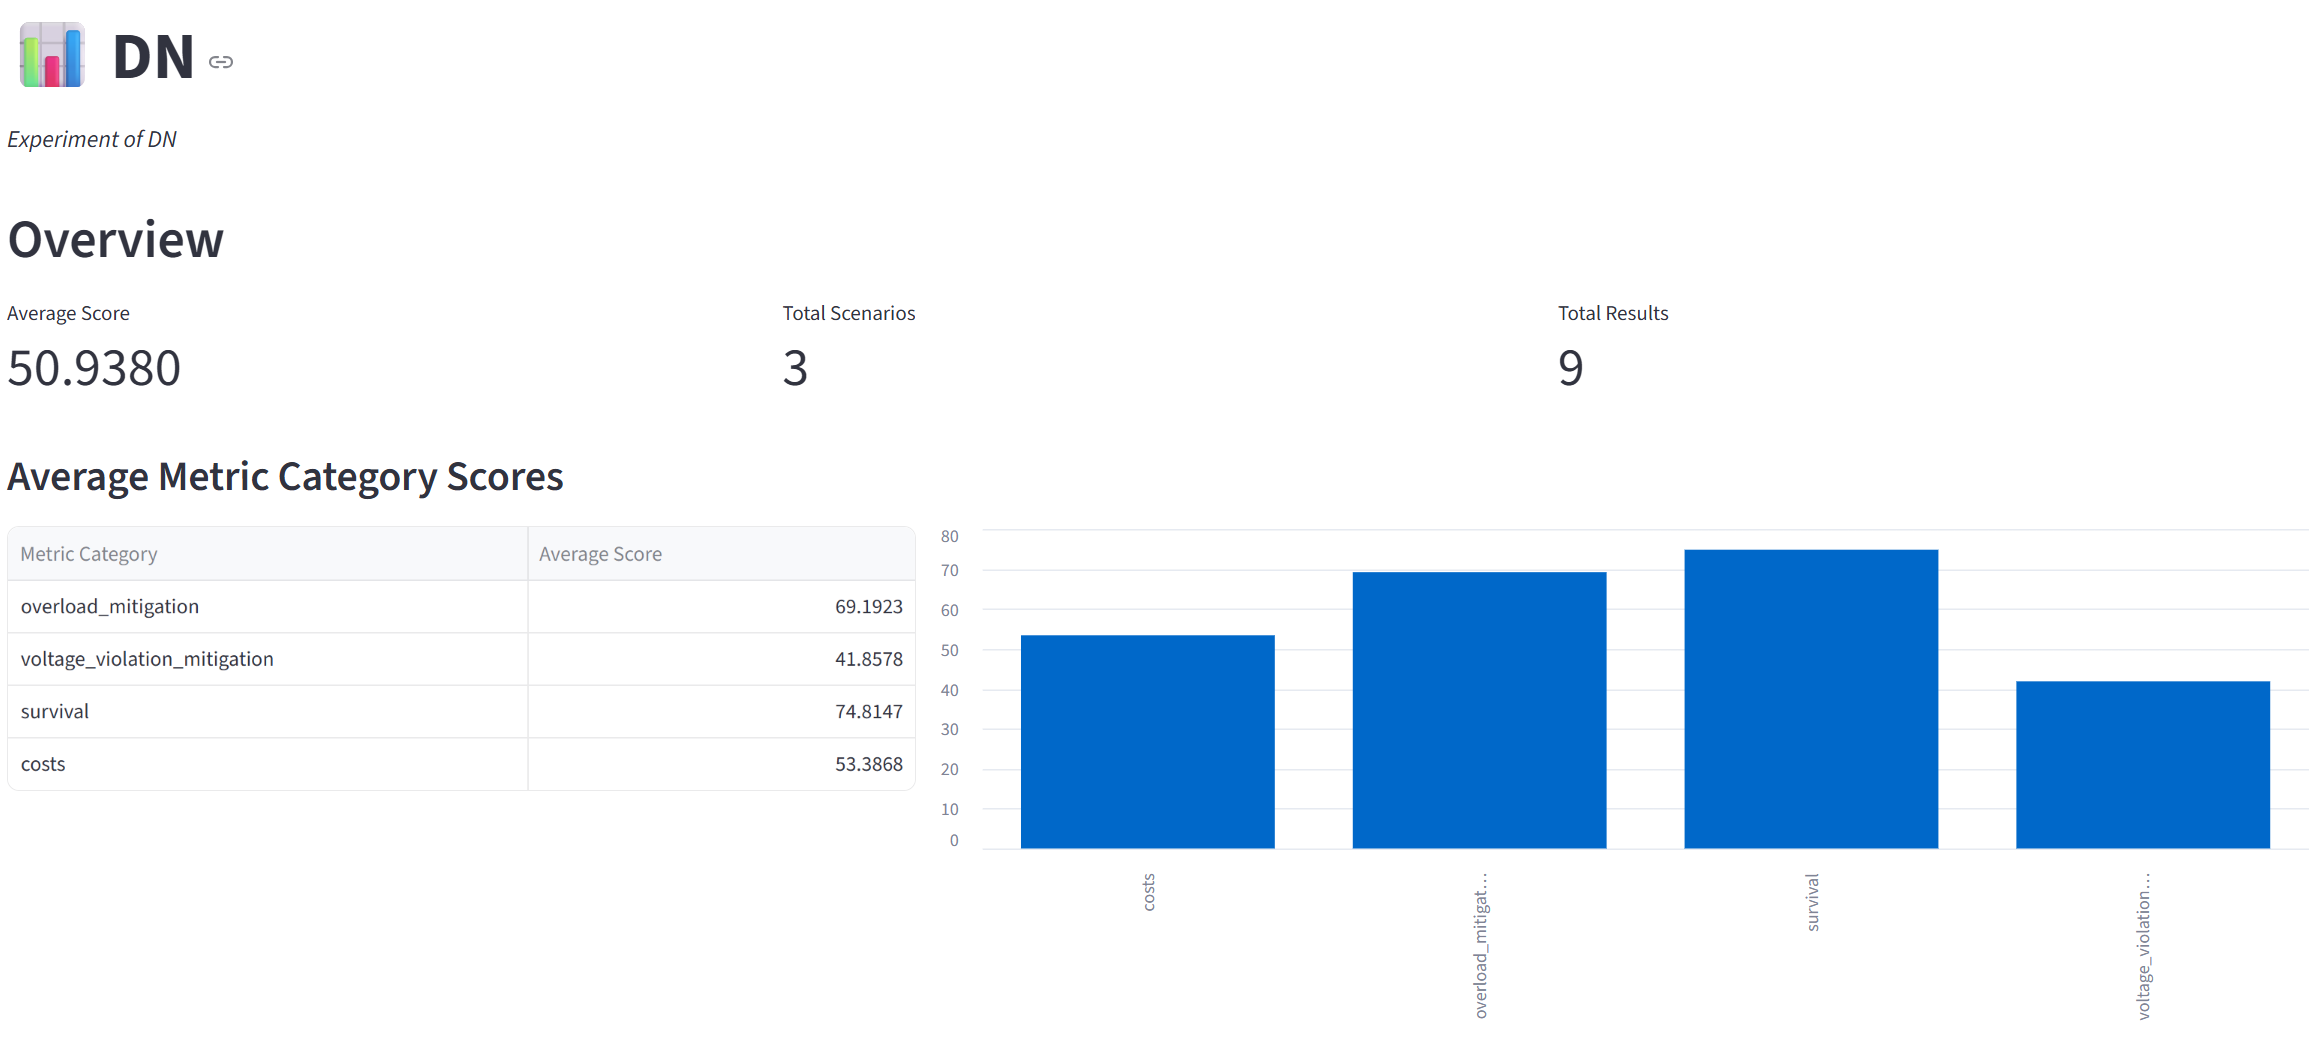
\includegraphics[width=\textwidth]{images/appendix/webapp/webapp_overview.png}
        \caption{Overview section}
        \label{fig:webapp-overview}
    \end{subfigure}

    \vspace{0.1em}

    \begin{subfigure}[t]{\textwidth}
        \centering
        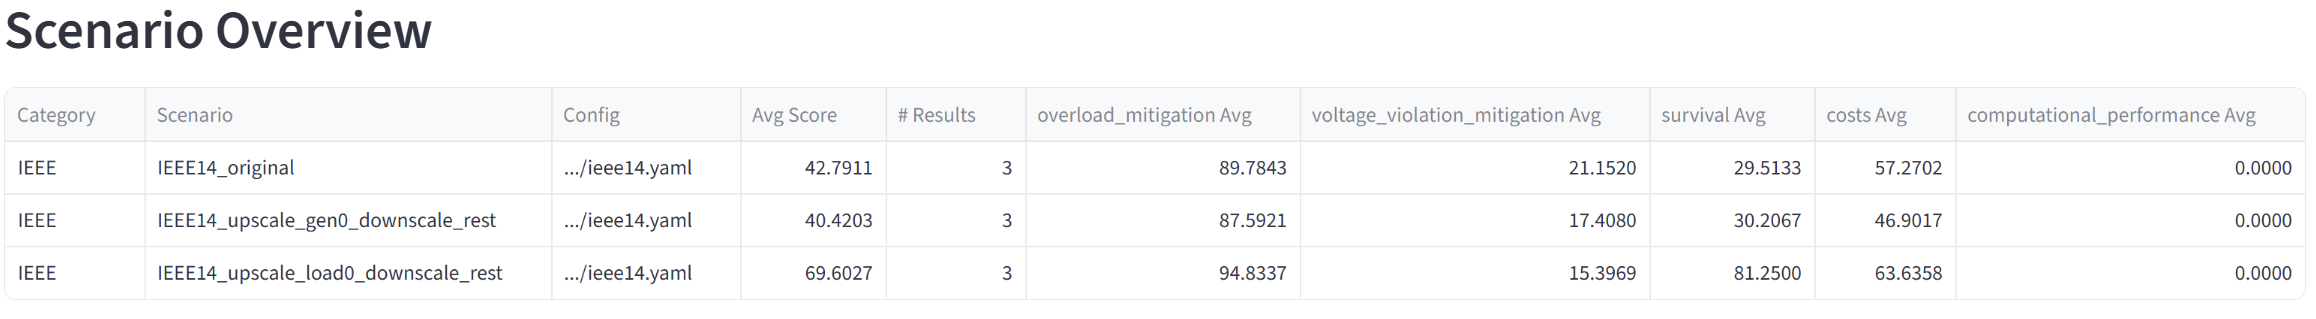
\includegraphics[width=\textwidth]{images/appendix/webapp/webapp_scenario_overview.png}
        \caption{Scenario overview section}
        \label{fig:webapp-scenario-overview}
    \end{subfigure}

    \vspace{0.1em}
    
    \begin{subfigure}[t]{\textwidth}
        \centering
        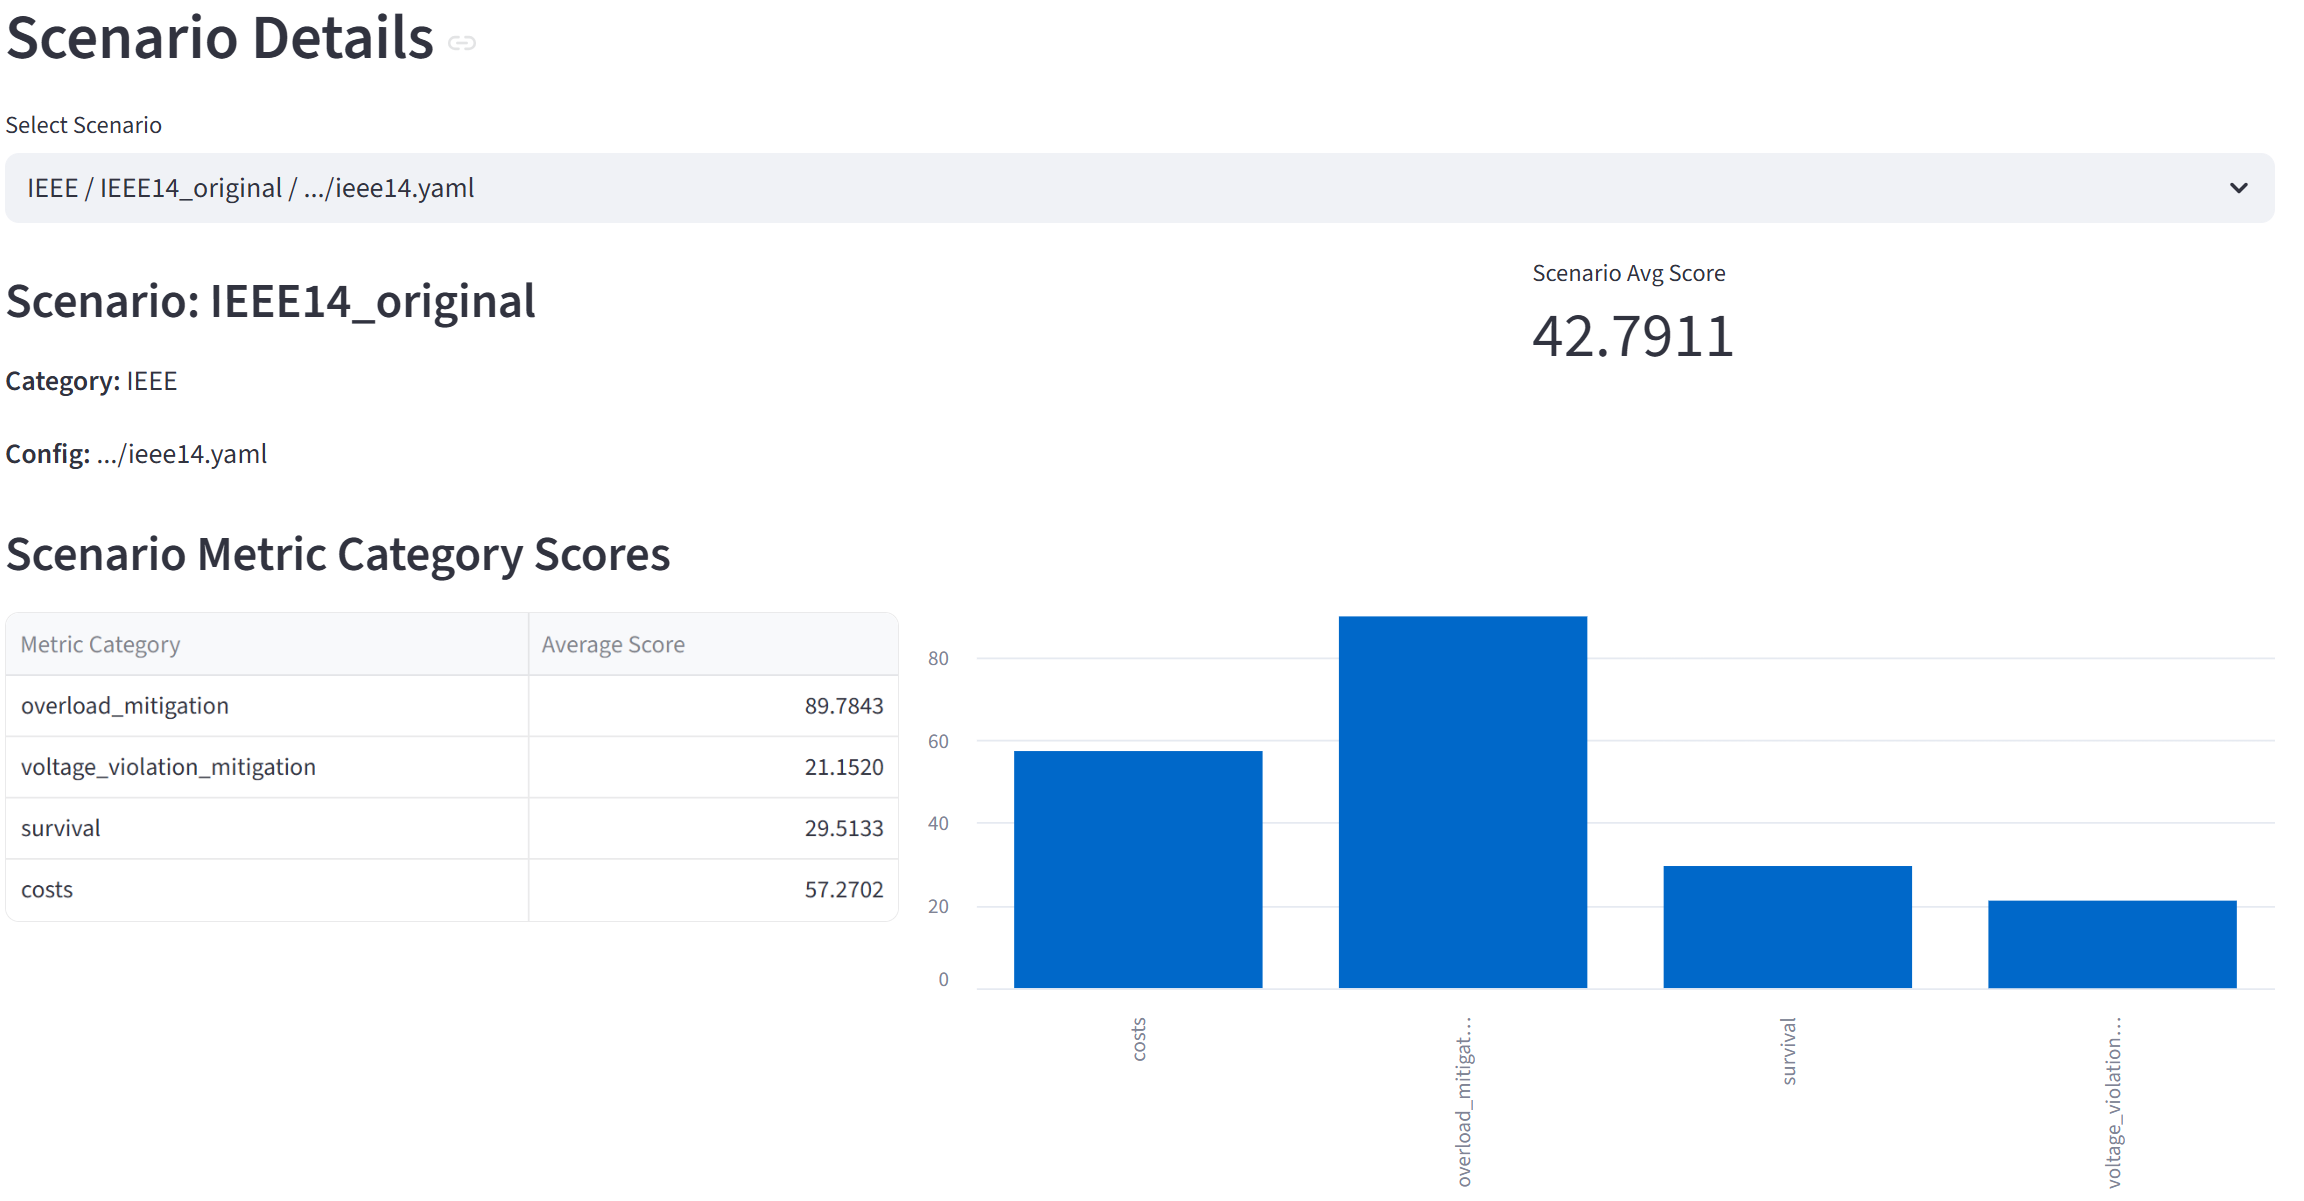
\includegraphics[width=\textwidth]{images/appendix/webapp/webapp_scenario_details.png}
        \caption{Scenario details section}
        \label{fig:webapp-scenario-details}
    \end{subfigure}

    \caption{Overview over webapp sections}
    \label{fig:webapp-screenshots}
\end{figure}

\begin{figure}[htp]
    \ContinuedFloat
    \centering

    \begin{subfigure}[t]{\textwidth}
        \centering
        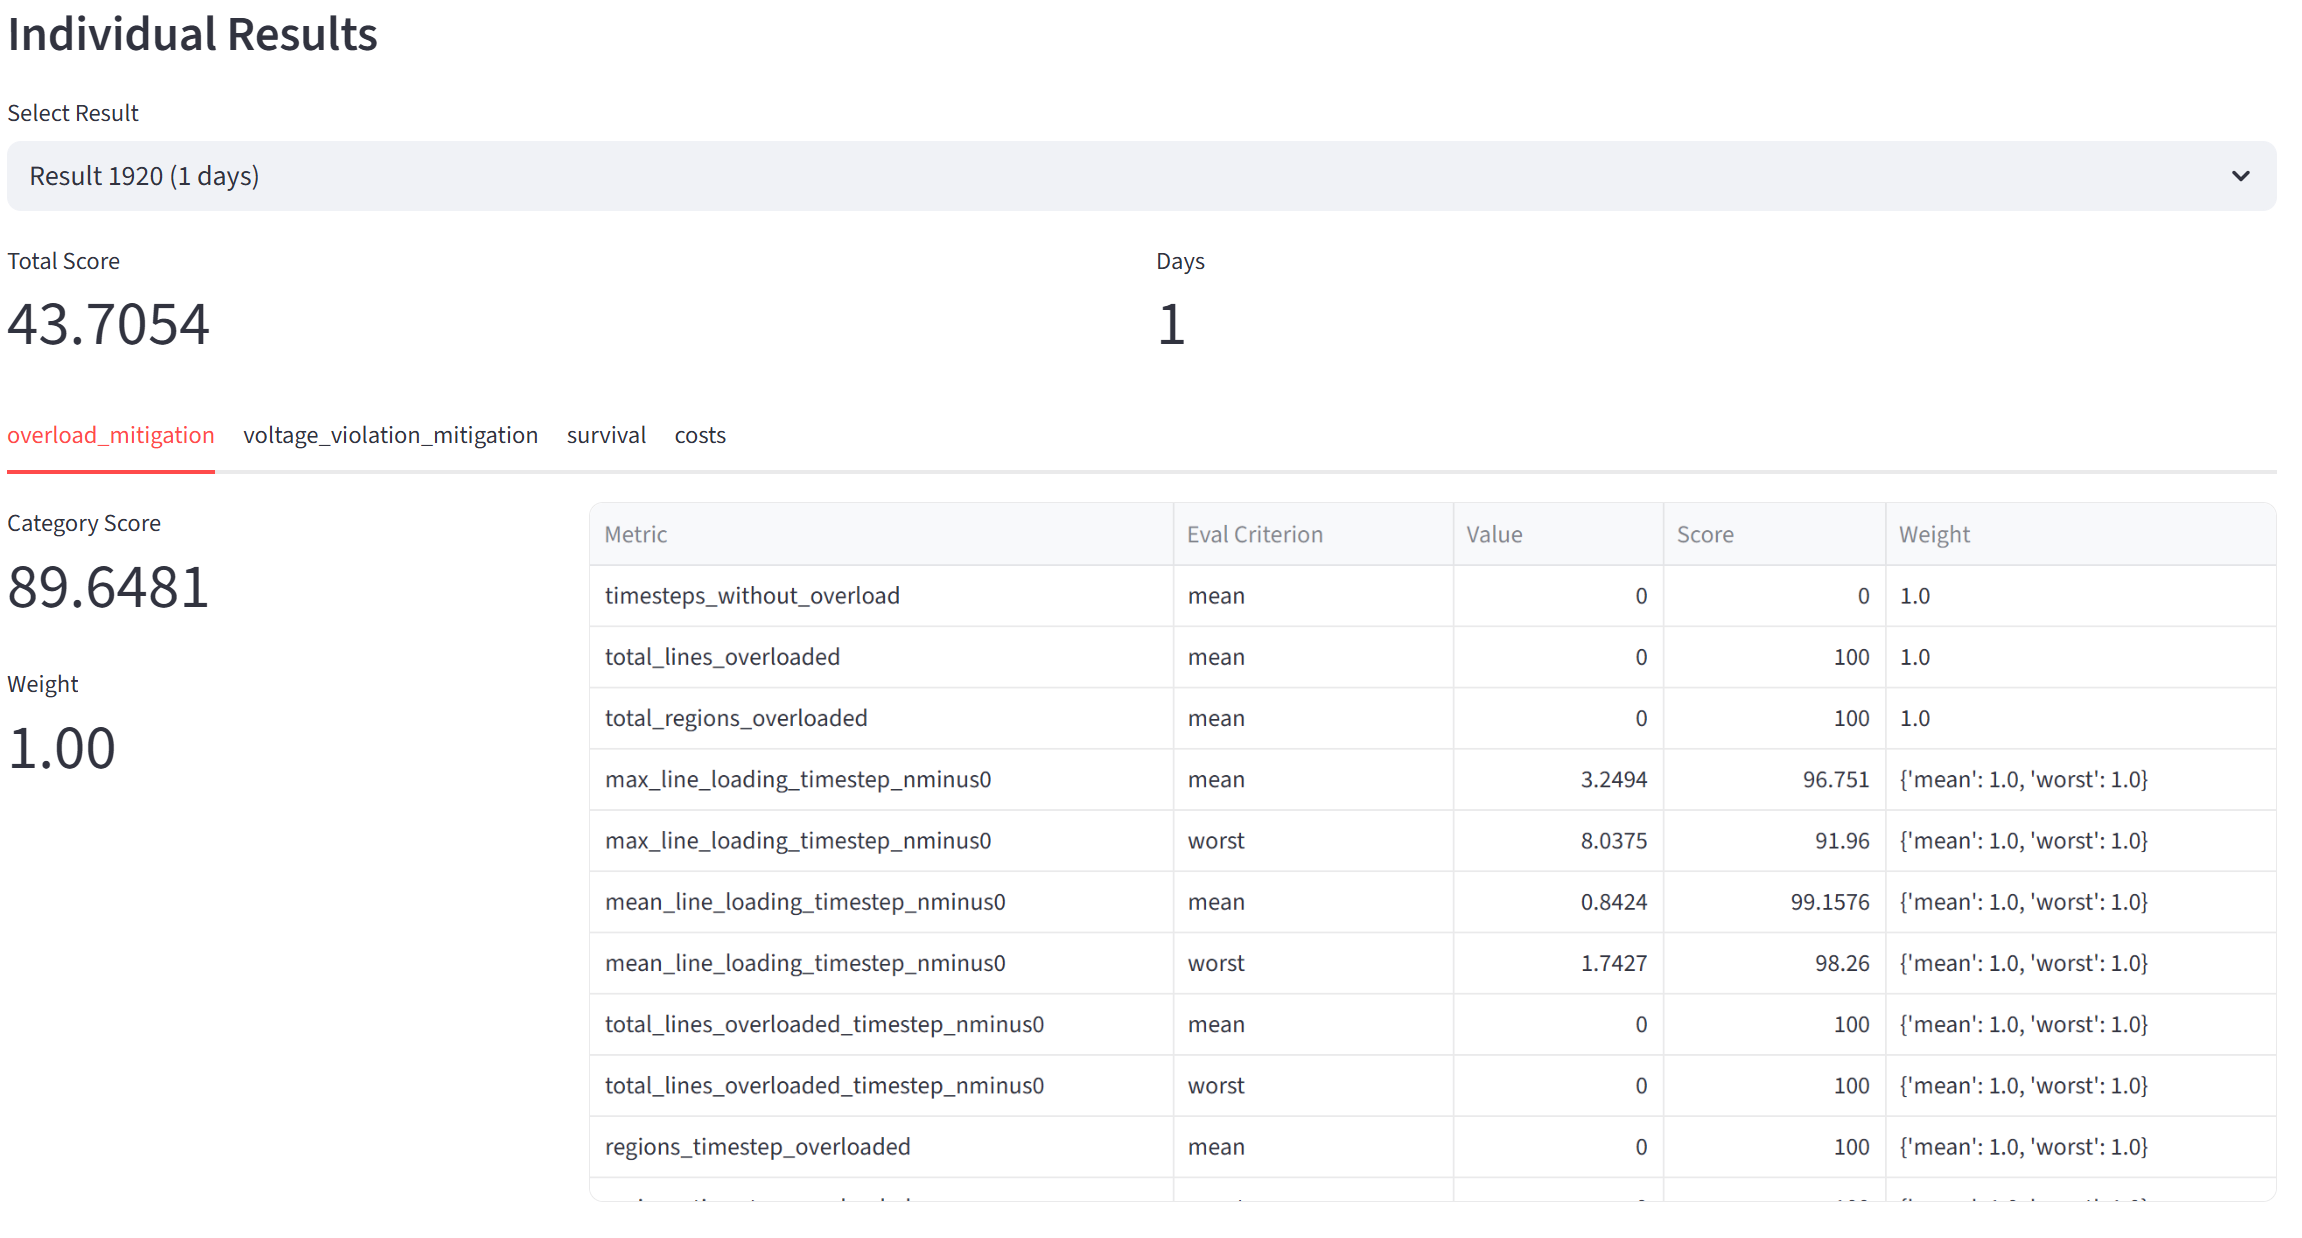
\includegraphics[width=\textwidth]{images/appendix/webapp/webapp_individual_results.png}
        \caption{Individual result section}
        \label{fig:webapp-individual-result}
    \end{subfigure}

    \caption{Overview over webapp sections (continued)}
\end{figure}


\FloatBarrier

\subsection{Summary Comparison Web Application}\label{app:comparison-webapp}
Figure \ref{fig:comparison-webapp-screenshots} shows screenshots of the Streamlit-based comparison web application, which is introduced in Section \ref{ssec:visual-feedback}.

\begin{figure}[htp]
    \centering
    \begin{subfigure}[t]{0.98\textwidth}
        \centering
        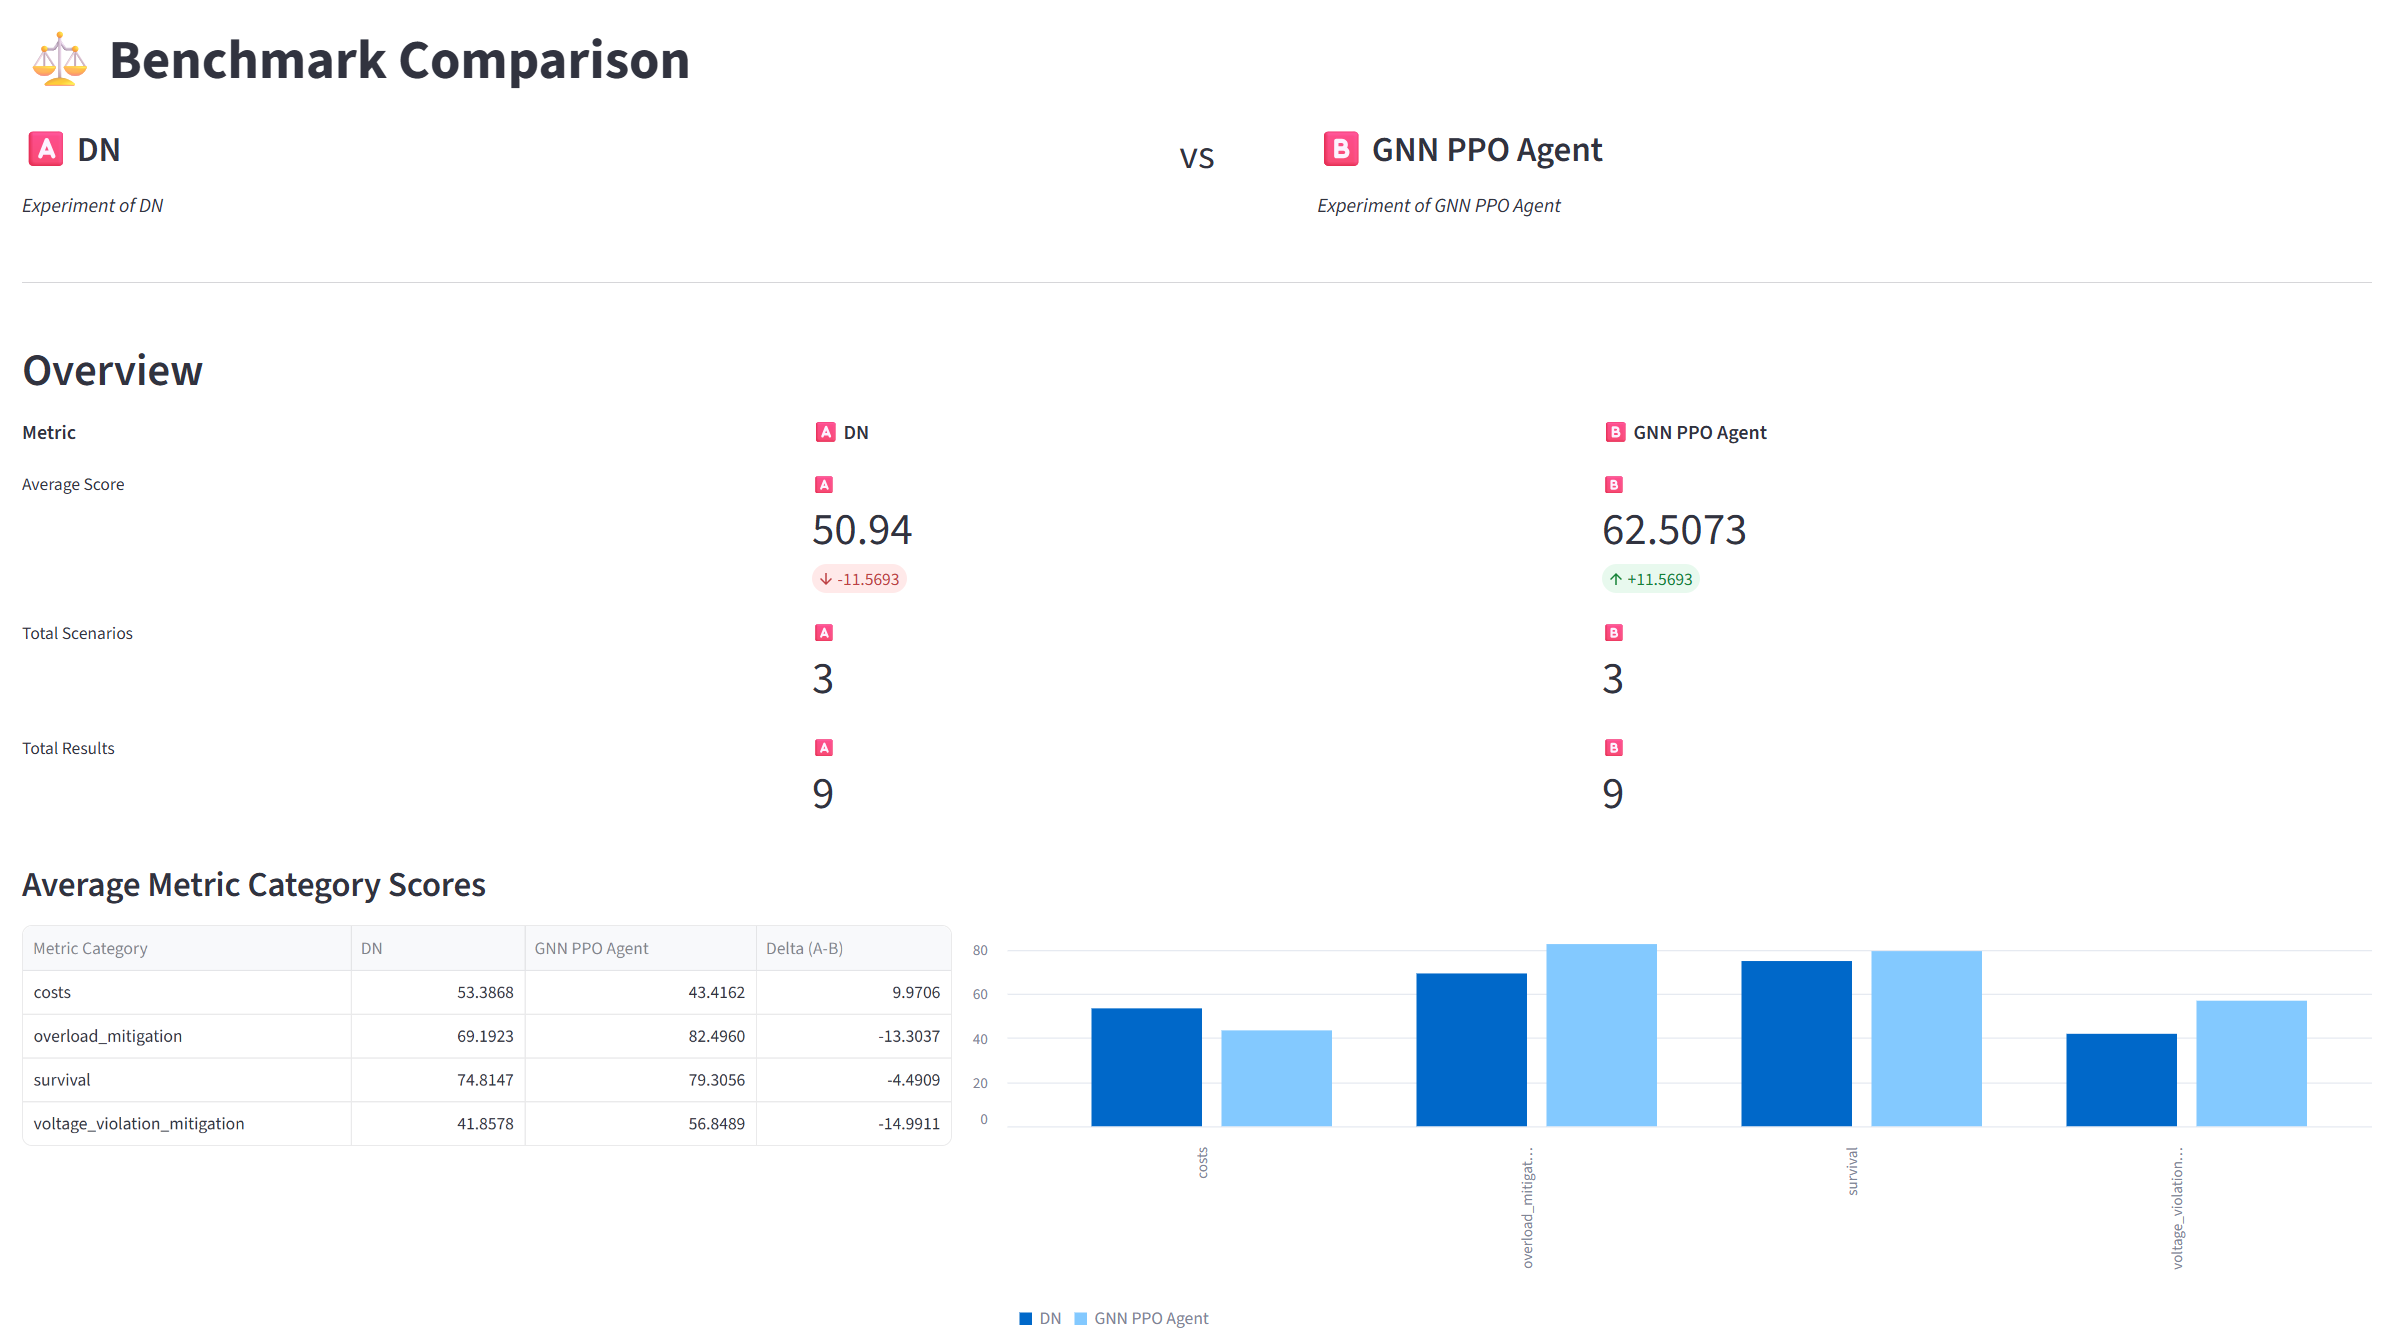
\includegraphics[width=\textwidth]{images/appendix/webapp/comparison_overview.png}
        \caption{Overview section}
        \label{fig:comparison-overview}
    \end{subfigure}

    \caption{Overview over comparison webapp sections, with do-nothing agent on the left, and a PPO agent on the right}
    \label{fig:comparison-webapp-screenshots}
\end{figure}

\begin{figure}[htp]
    \ContinuedFloat
    \centering

    \begin{subfigure}[t]{0.98\textwidth}
        \centering
        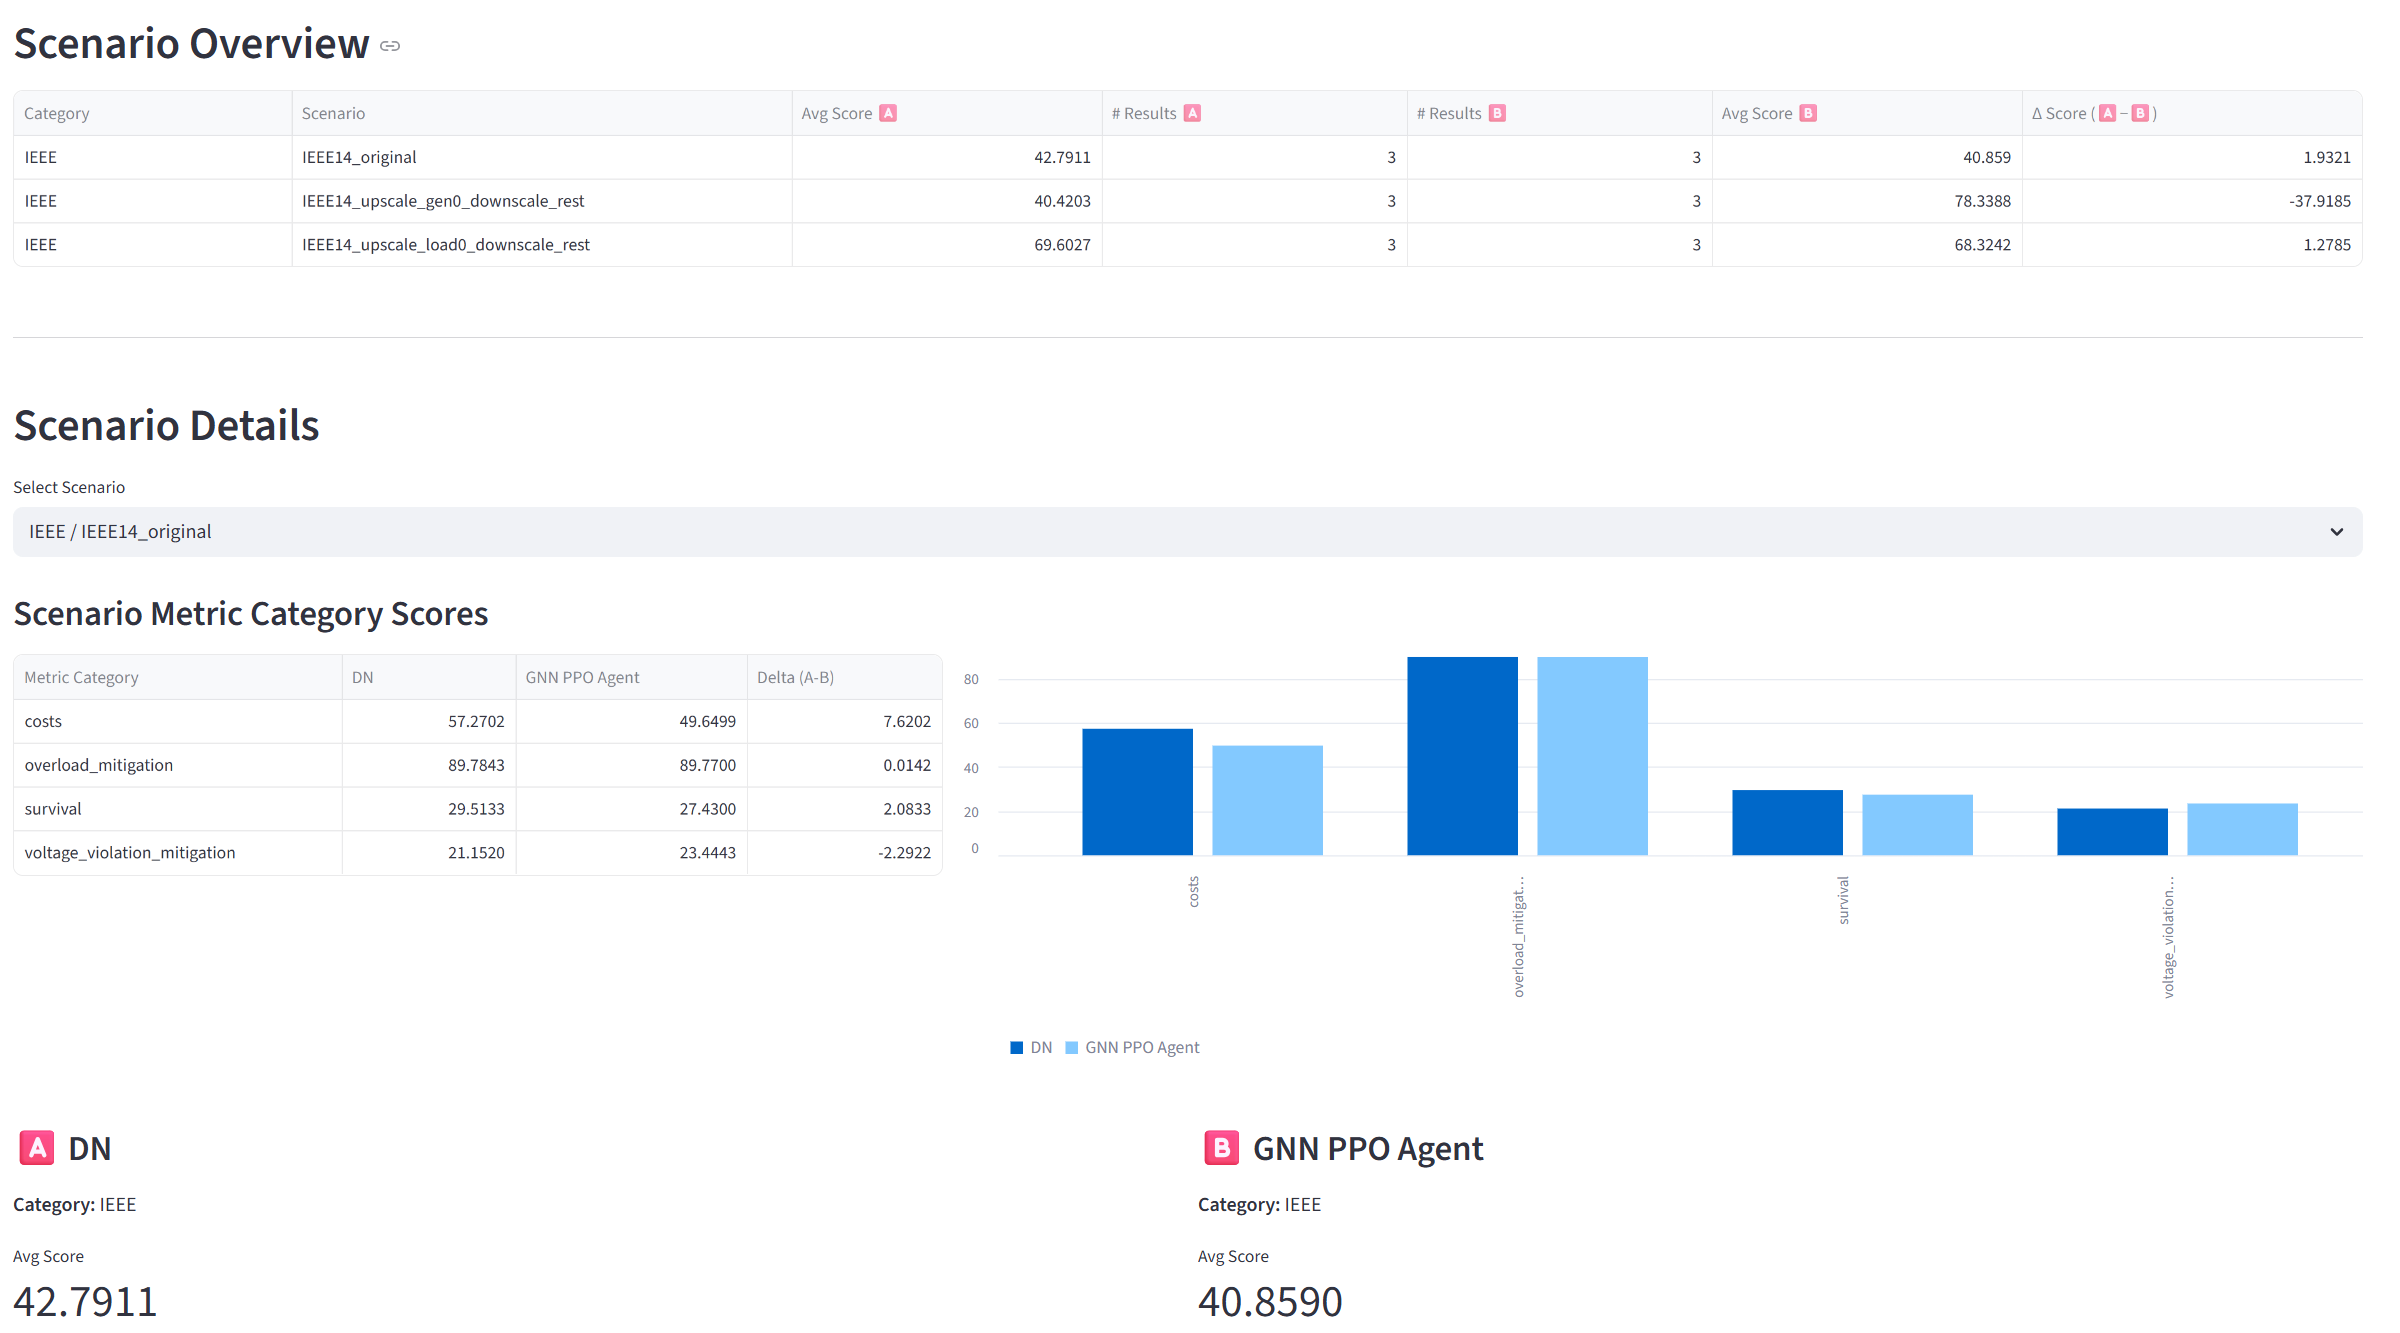
\includegraphics[width=\textwidth]{images/appendix/webapp/comparison_scenario_overview.png}
        \caption{Scenario overview section}
        \label{fig:comparison-scenario-overview}
    \end{subfigure}

    \vspace{0.1em}

    \begin{subfigure}[t]{0.98\textwidth}
        \centering
        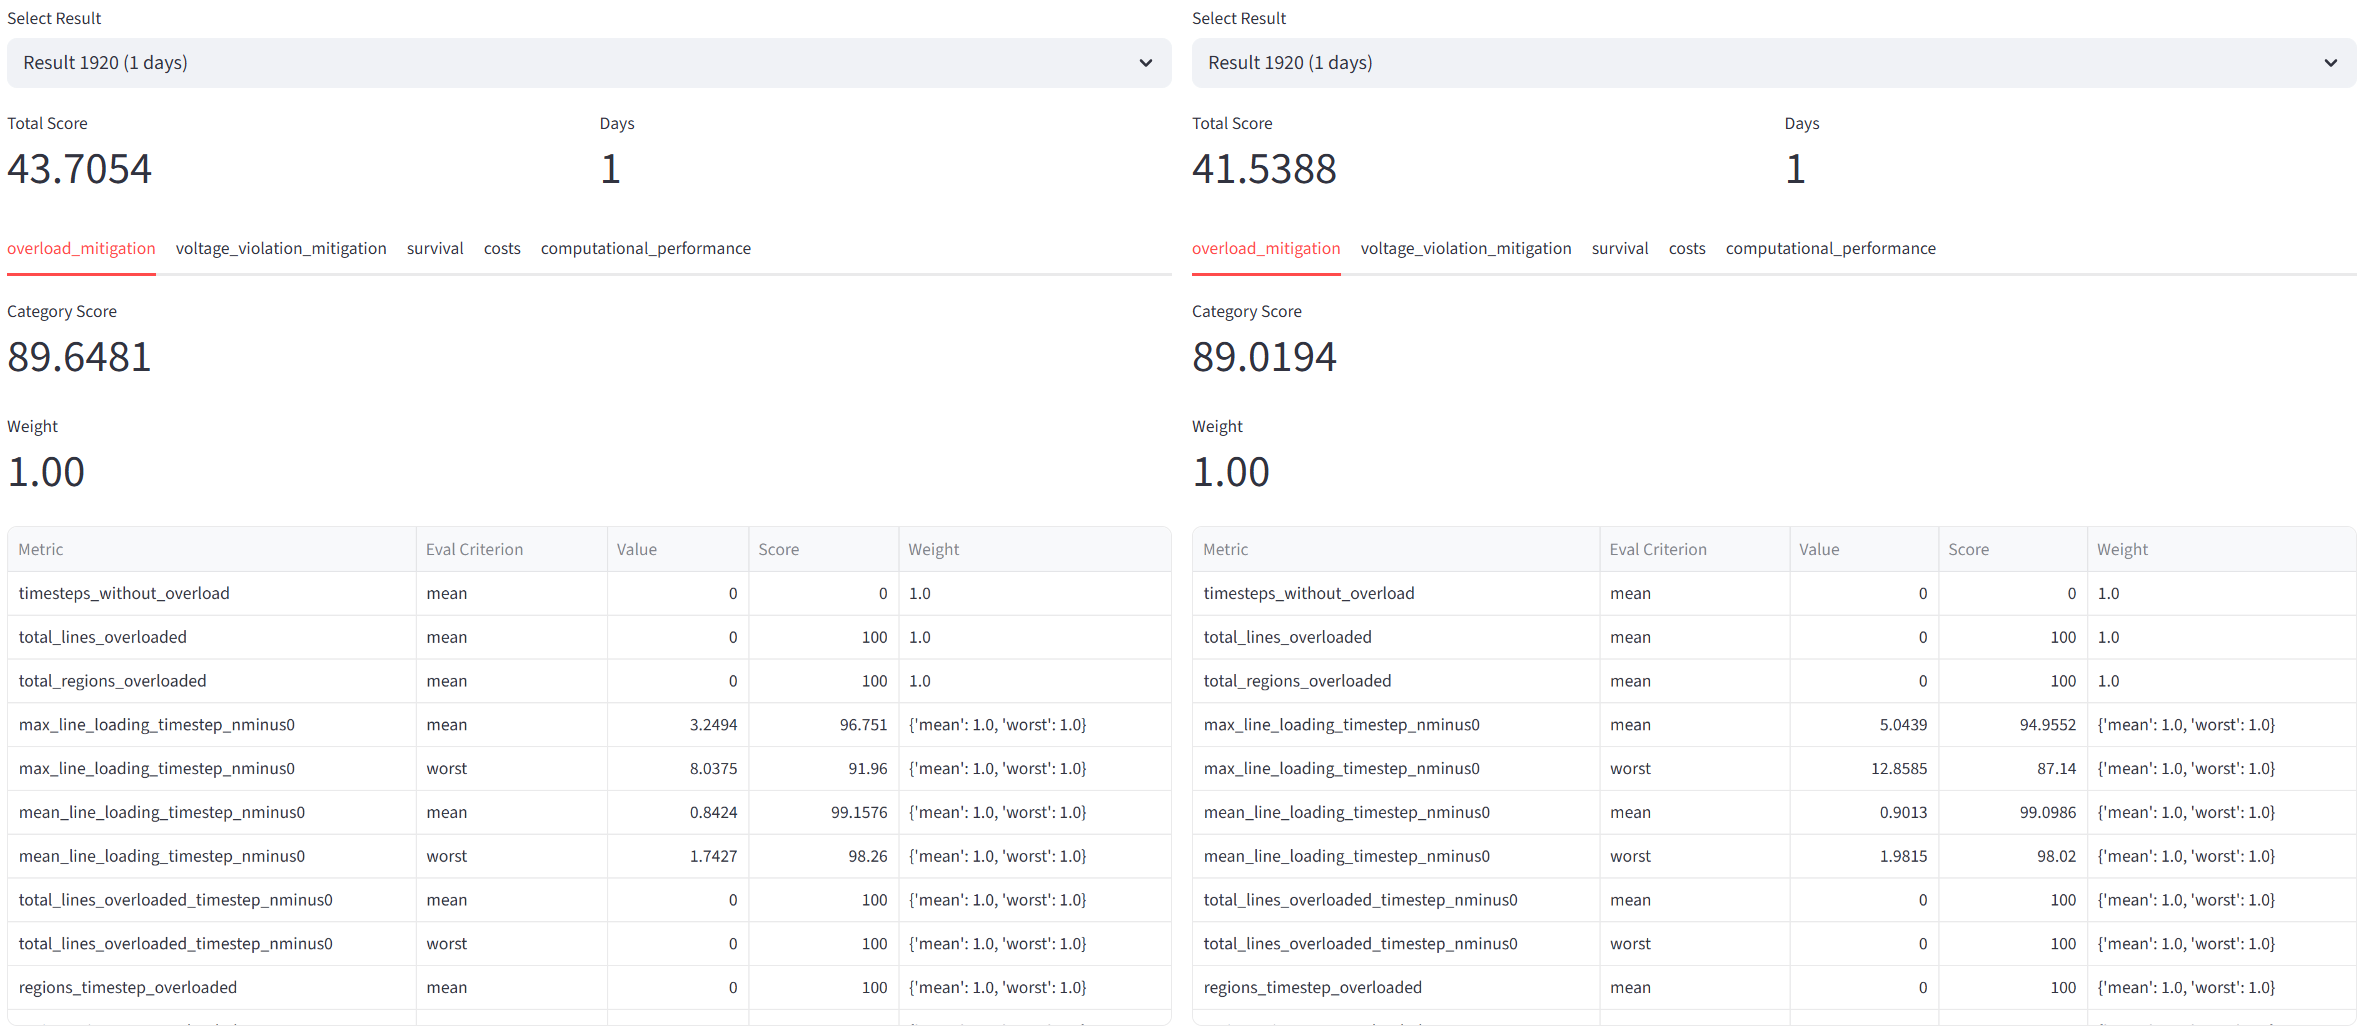
\includegraphics[width=\textwidth]{images/appendix/webapp/comparison_individual_results.png}
        \caption{Individual result section}
        \label{fig:comparison-individual-result}
    \end{subfigure}

    \caption{Overview over comparison webapp sections, with do-nothing agent on the left, and a PPO agent on the right (continued)}
\end{figure}

\FloatBarrier

\subsection{Replay Graphs}
Figure \ref{fig:replay-graphs} shows an example of the two graph views generated by the replay task described in Section \ref{ssec:replay-data}.

\begin{figure}[htp]
    \centering
    \begin{subfigure}[t]{0.9\textwidth}
        \centering
        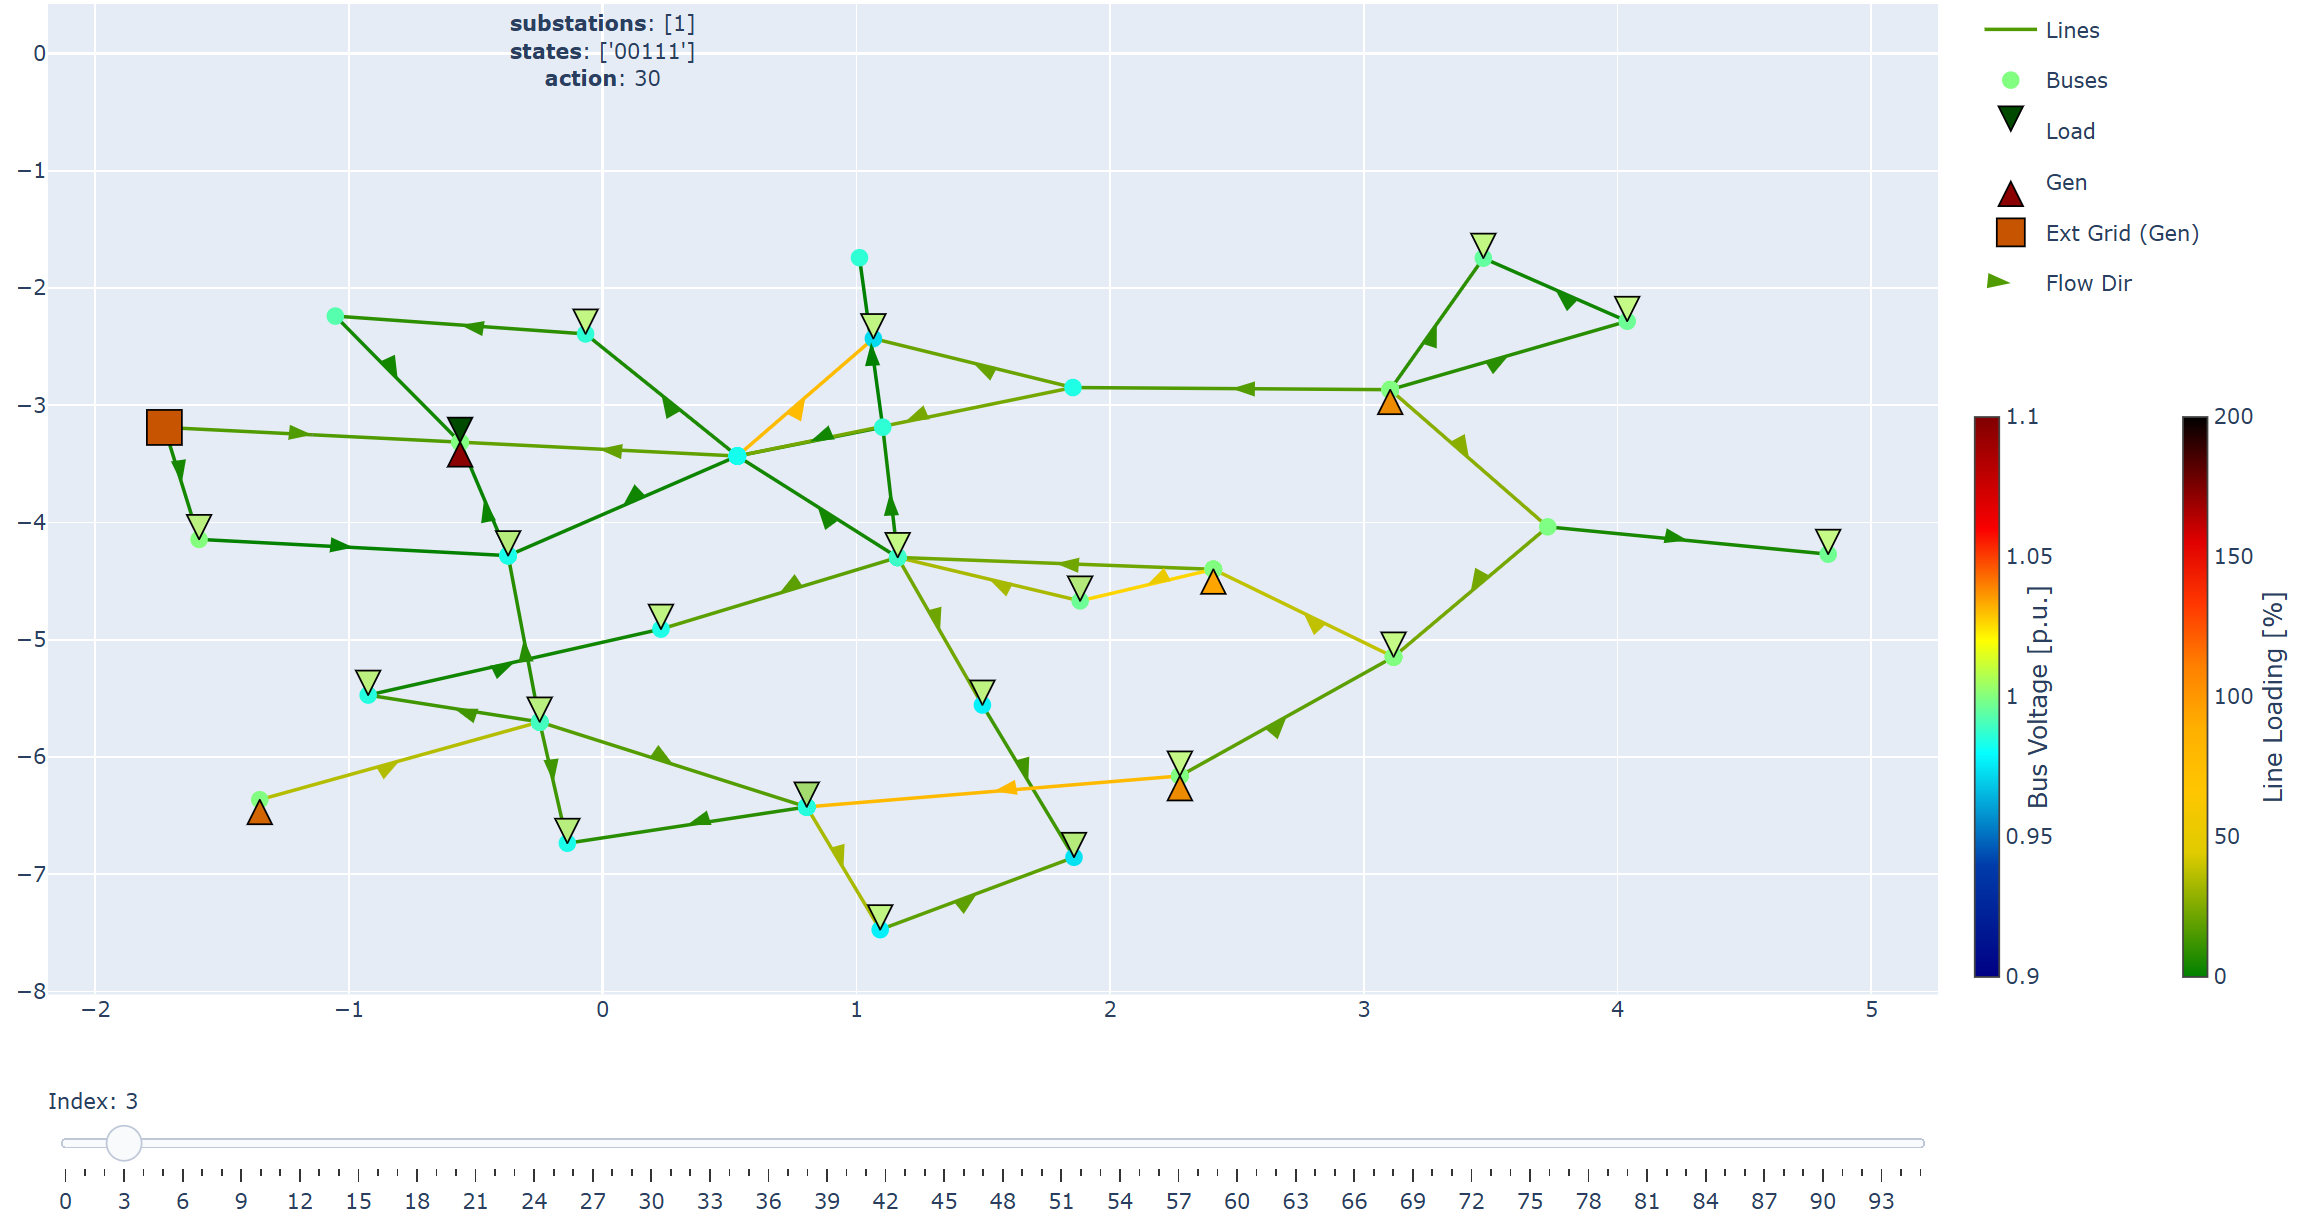
\includegraphics[width=\textwidth]{images/appendix/replay/network_graph.png}
        \caption{Network graph of the replay data, showing the limits of the grid}
        \label{fig:network-graph}
    \end{subfigure}

    \vspace{0.1em}

    \begin{subfigure}[t]{0.9\textwidth}
        \centering
        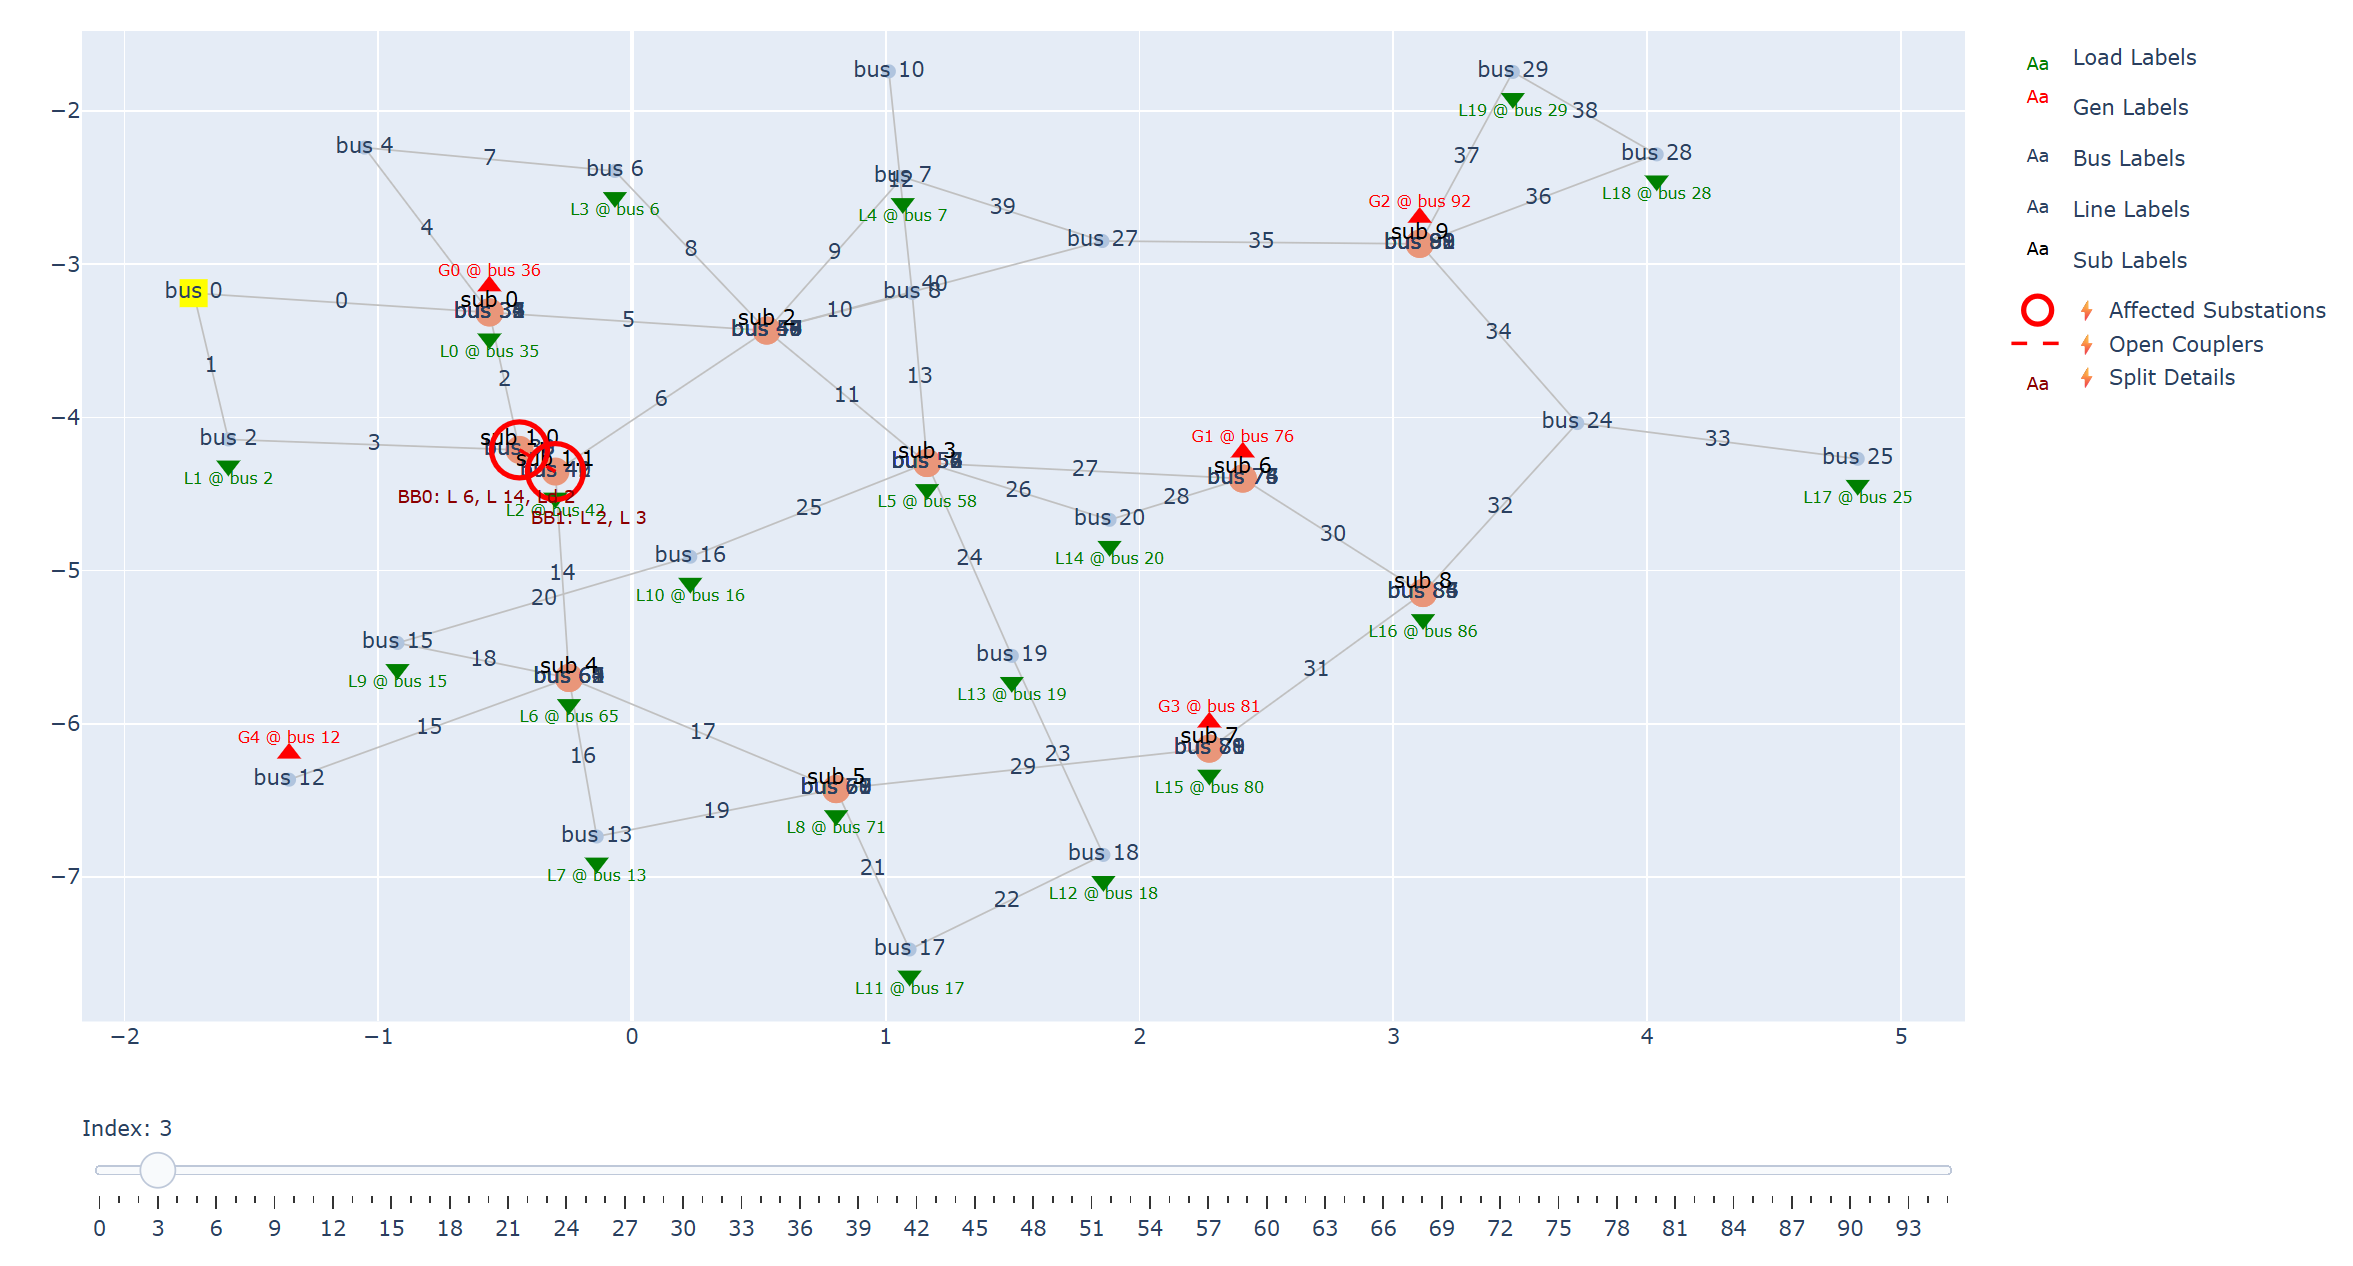
\includegraphics[width=\textwidth]{images/appendix/replay/action_graph.png}
        \caption{Action graph of the replay data, showing the actions of the agent}
        \label{fig:action-graph}
    \end{subfigure}

    \vspace{0.1em}

    \begin{subfigure}[t]{0.48\textwidth}
        \centering
        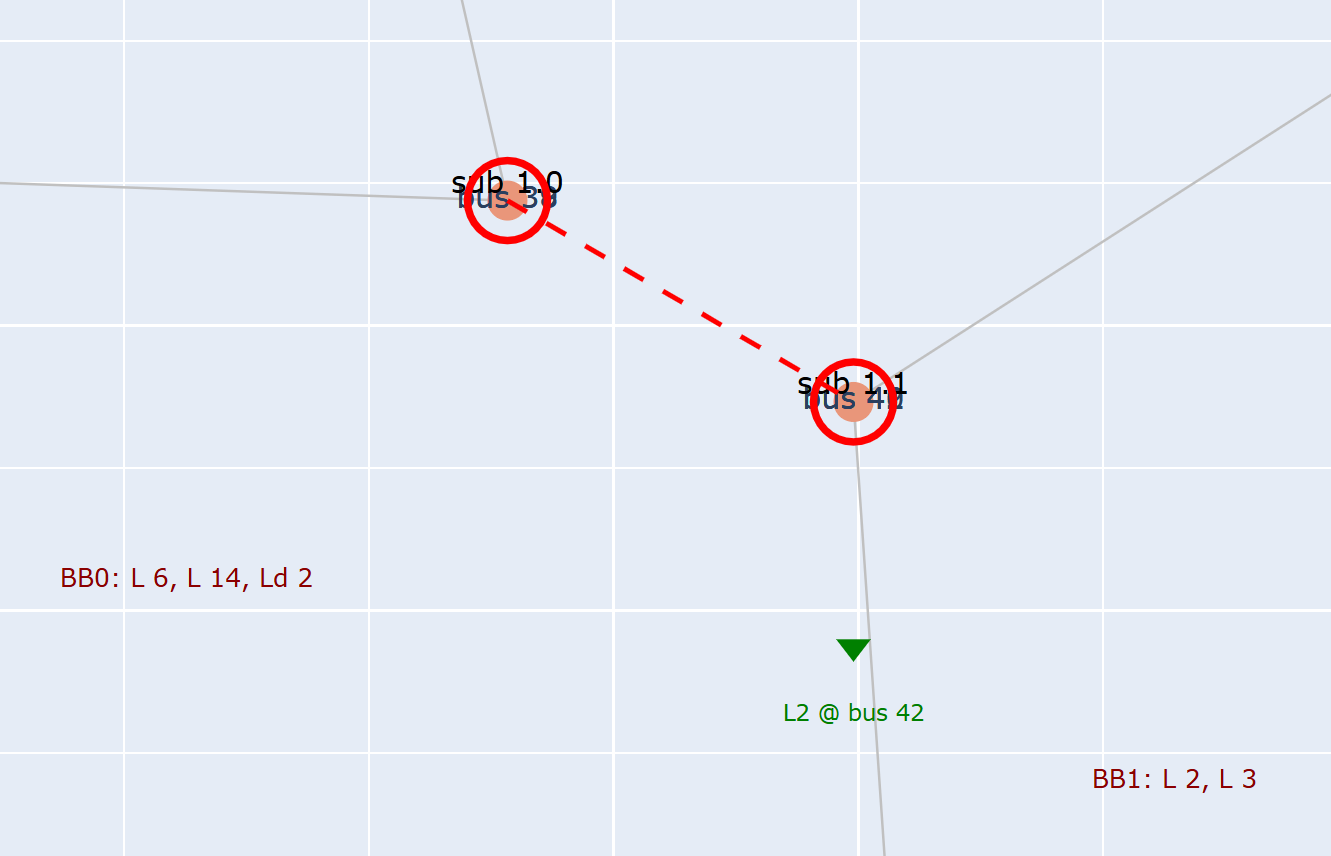
\includegraphics[width=\textwidth]{images/appendix/replay/action_graph_zoomed.png}
        \caption{Zoom-in of the action graph, showing bus-splitting}
        \label{fig:action-graph-zoomed}
    \end{subfigure}

    \caption{Overview over the replay data website, showing the two graph views}
    \label{fig:replay-graphs}
\end{figure}
    \chapter{Experiment Setup}\label{ch:exp-setup}
This appendix provides supplementary tables and figures for the experimental setup described in Section \ref{sec:experiment_setup}. Section \ref{sec:exp-reward-setup} documents the exact reward configuration used by the greedy agent and during \ac{ppo} training. Section \ref{sec:exp-scenario-setup} shows the two evaluated power grids with their modified components highlighted, together with a full listing of all chosen scenarios and evaluation indices. Finally, Section \ref{sec:exp-ppo-setup} lists the tunable hyperparameters of the \ac{gnn}-based \ac{ppo} agent, the final tuned values for each scenario, and the results of the corresponding training runs.

\section{Reward Setup}\label{sec:exp-reward-setup}
Table \ref{tab:reward_settings} lists the metrics and their assigned weights used to compute the reward signal for the greedy agent's action selection and for training the \ac{ppo} agent, as introduced in Section \ref{sec:agent-integration}. The corresponding worst-case and best-case reference values used to normalise each metric are fixed and listed in Table \ref{tab:reward_metrics}.

\begin{table}[htbp]
  \centering
  \small
  \caption{Reward configuration used in all experiments}
  \label{tab:reward_settings}
  \begin{tabular}{lc}
    \toprule
    Metric & Weight $w_i$  \\
    \midrule
    Maximum line loading $N\!-\!0$ & 3 \\
    Number of overloaded lines $N\!-\!0$ & 1 \\
    \midrule
    Non-convergence penalty $r_{\mathrm{fail}}$ & $-2$ \\
    \bottomrule
  \end{tabular}
\end{table}

\FloatBarrier










\section{Scenario Setup}\label{sec:exp-scenario-setup}
This section documents the two power grids and all scenarios evaluated in the experiments, complementing the description given in Section \ref{sec:experiment_setup}.

\subsection{Evaluated Power Grids}
Figure \ref{fig:exp-grids} shows the two IEEE test grids used throughout the experiments, with the components affected by scenario-specific modifications, such as scaled generators or loads, highlighted directly on the grid layout.

\begin{figure}[htp]
    \centering
    \begin{subfigure}[b]{0.8\textwidth}
        \centering
        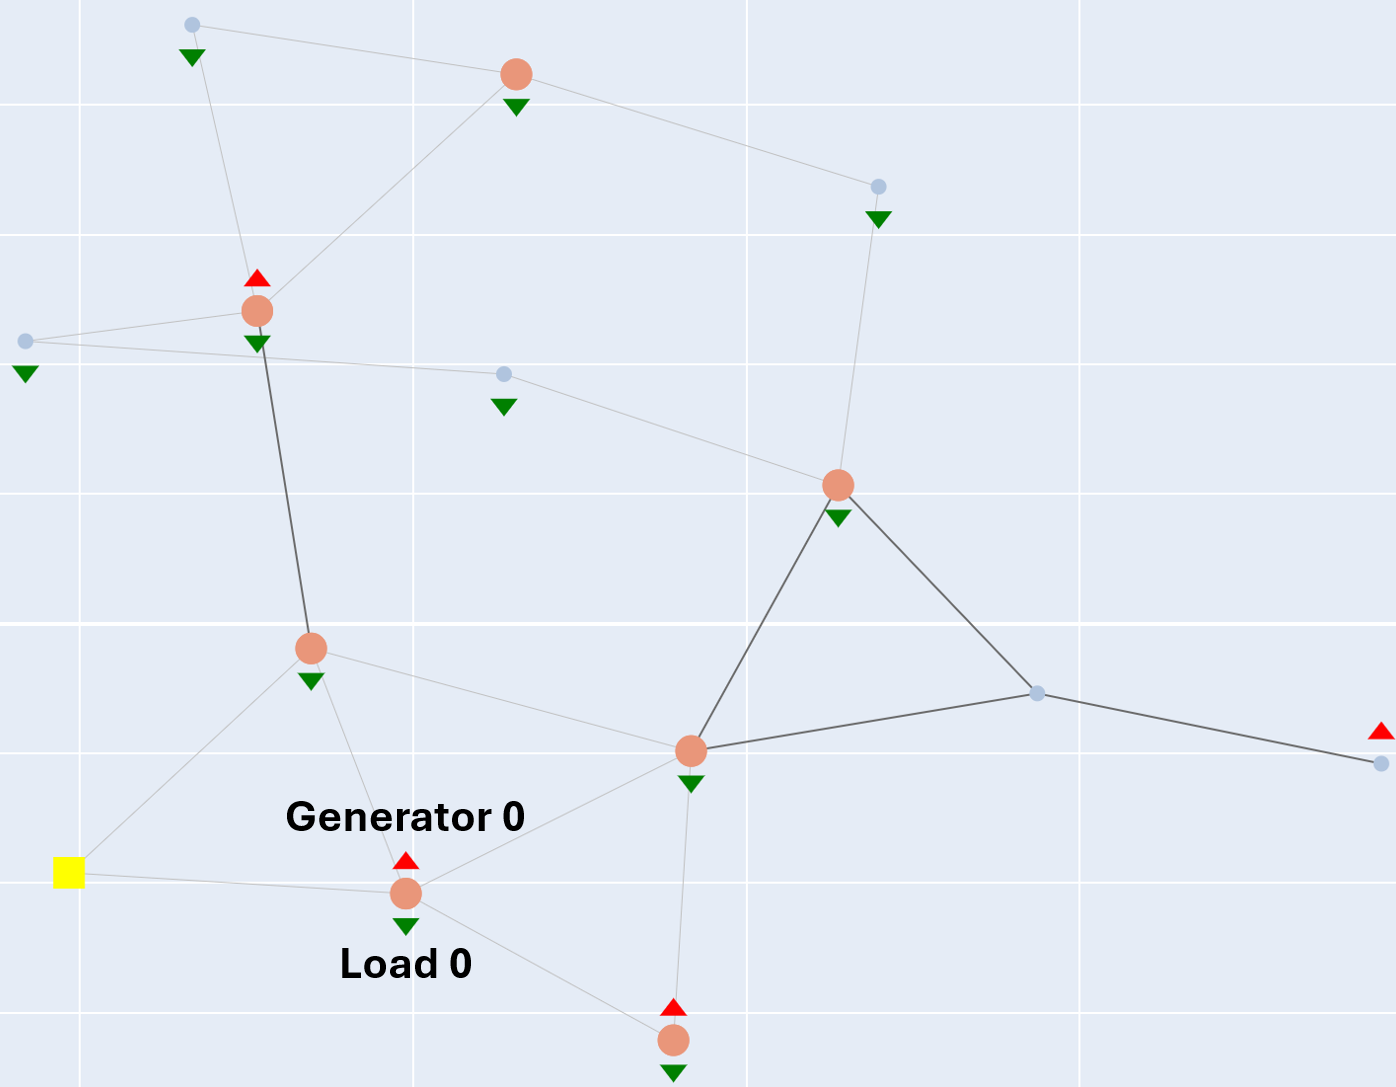
\includegraphics[width=\textwidth]{images/experiments/grids/14b.png}
        \caption{IEEE 14-bus test grid}
        \label{fig:grid-14}
    \end{subfigure}

    \vspace{1em}

    \begin{subfigure}[b]{1\textwidth}
        \centering
        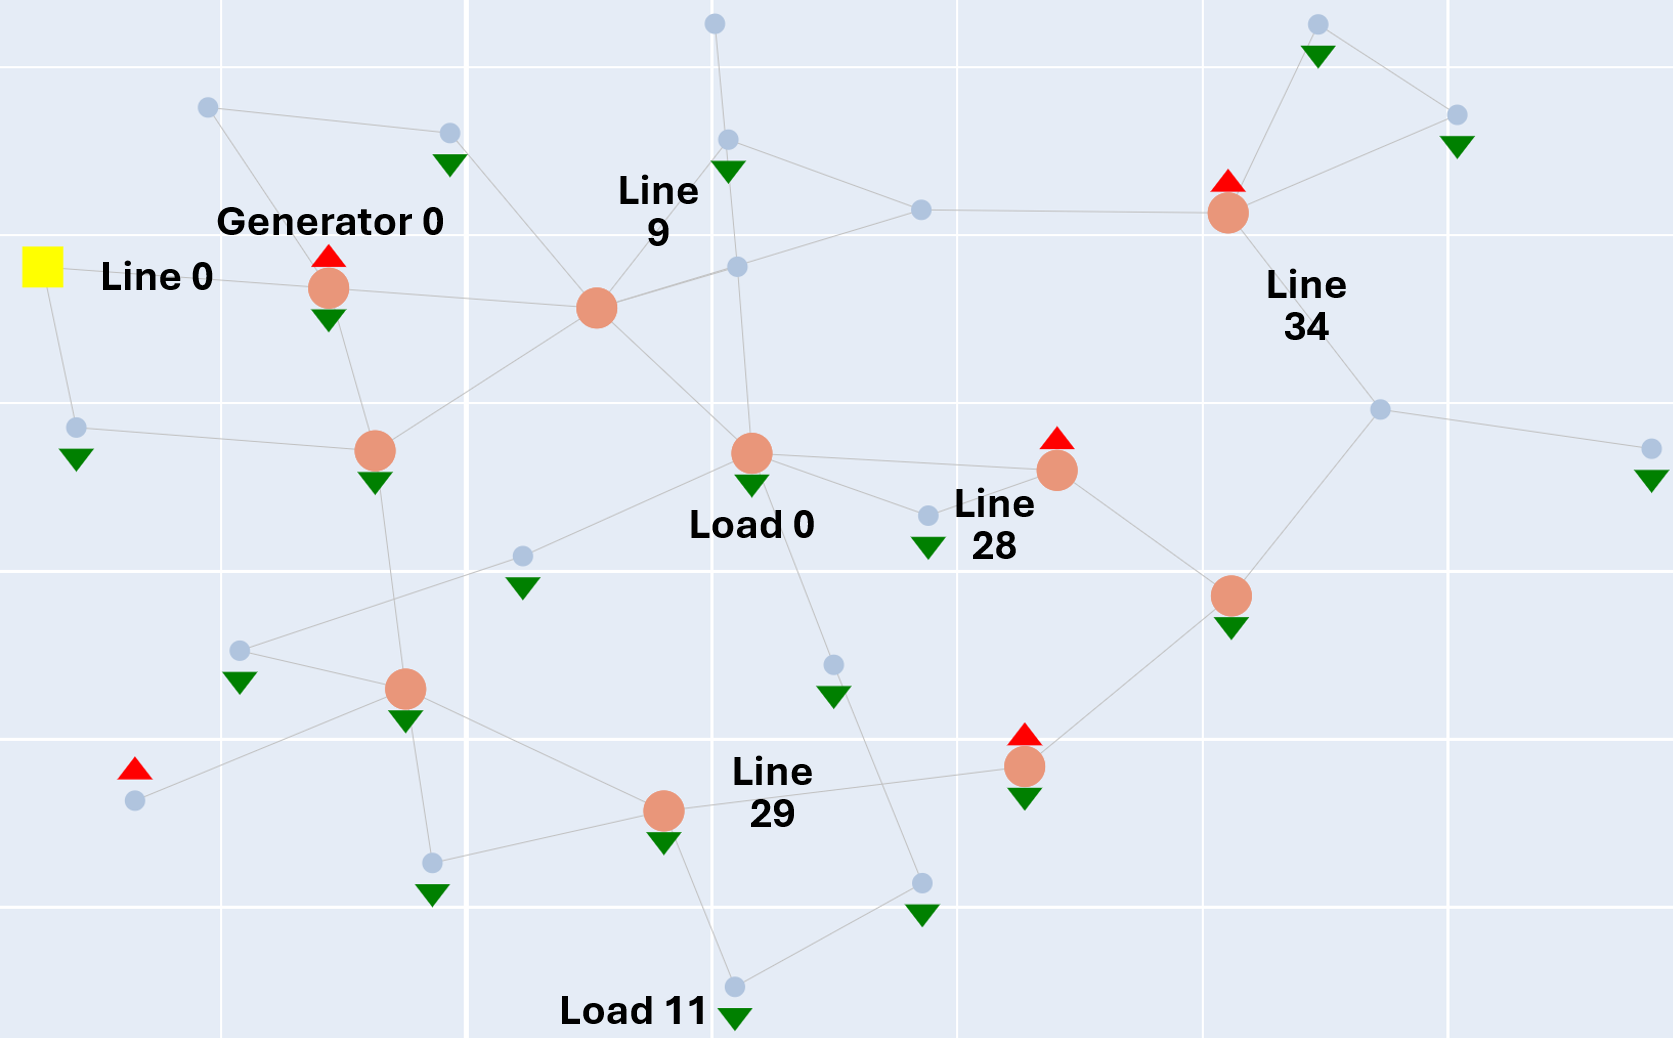
\includegraphics[width=\textwidth]{images/experiments/grids/30b.png}
        \caption{IEEE 30-bus test grid}
        \label{fig:grid-30}
    \end{subfigure}
    \caption{Power grids used in the experiments, with modified grid components identified by labels}
    \label{fig:exp-grids}
\end{figure}

\FloatBarrier

\subsection{Chosen Scenarios and Runs}
Table \ref{tab:scenarios-setup} lists all scenarios evaluated in the experiments, together with the profile day indices selected for each run and a short description of the modifications applied to the respective base grid, as introduced in Section \ref{sec:experiment_setup}.

\begin{table}[htbp]
\centering
\small
\renewcommand{\arraystretch}{1.3}
\begin{tabular}{|l|p{4.6cm}|p{6cm}|}
\hline
\textbf{Scenario Name} & \textbf{Index} & \textbf{Description} \\
\hline
14B\_ORIG & 1920, 8640, 21120 (days 20, 90, 220) & Unmodified 14-bus IEEE test case \\
\hline
14B\_UP\_GN0 & 3840, 18240, 26880 (days 40, 190, 280) & 14-bus case, active power generation of generator 0 scaled by $5\times$ (original 420\,MW) \\
\hline
14B\_UP\_LD0 & 3840, 11520, 5760 (days 40, 120, 60) & 14-bus case, active and reactive power of load 0 scaled by $15\times$ (original 65-70\,MW)\\
\hline
14B\_UP\_GN0- & 3840, 18240, 26880 (days 40, 190, 280) & As 14B\_UP\_GN0, but with a lower scaling factor of $2.5\times$ \\
\hline
14B\_UP\_GN0+ & 3840, 18240, 26880 (days 40, 190, 280) & As 14B\_UP\_GN0, but with a higher scaling factor of $7.5\times$ \\
\hline
14B\_UP\_LD0- & 3840, 11520, 5760 (days 40, 120, 60) & As 14B\_UP\_LD0, but with a lower scaling factor of $5\times$ \\
\hline
14B\_UP\_LD0+ & 3840, 11520, 5760 (days 40, 120, 60) & As 14B\_UP\_LD0, but with a higher scaling factor of $25\times$ \\
\hline
30B\_ORIG & 27840 (day 290) & Unmodified 30-bus IEEE test case \\
\hline
30B\_UP\_LD5 & 12480, 13440, 30720 (days 130, 140, 320) & 30-bus case, active and reactive power of load 5 scaled by $20\times$ (original 3\,MW) \\
\hline
30B\_UP\_LD11 & 10560, 13440, 27840 (days 110, 140, 290) & 30-bus case, active and reactive power of load 11 scaled by $20\times$ (original 3\,MW) \\
\hline
30B\_MT\_LN & 27840 (day 290) & 30-bus case, year-long maintenance outage of lines 0, 9, 28, 29 and 34 \\
\hline
30B\_MT\_GN & 27840 (day 290) & 30-bus case, year-long maintenance outage of generator 0 \\
\hline
30B\_RC\_LN & 27840 (day 290) & 30-bus case, thermal capacity of lines 0, 9, 28, 29 and 34 reduced to 25\,\% \\
\hline
30B\_RC\_LN- & 27840 (day 290) & As 30B\_RC\_LN, but with a milder reduction to 50\,\% \\
\hline
30B\_RC\_LN+ & 27840 (day 290) & As 30B\_RC\_LN, but with a stronger reduction to 10\,\% \\
\hline
\end{tabular}
\caption{Overview of the scenarios and their evaluation indices for each run}
\label{tab:scenarios-setup}
\end{table}

\FloatBarrier












\section{PPO Setup}\label{sec:exp-ppo-setup}
This section documents the hyperparameters of the \ac{gnn}-based \ac{ppo} agent introduced in Section \ref{ssec:custom-agent-setup}, the final values selected for each scenario by the \texttt{OptunaTuner}, and the outcome of the corresponding training runs.

\subsection{Hyperparameters}
Table \ref{tab:ppo-hparams} lists and briefly describes all tunable hyperparameters of the \ac{gnn}-based \ac{ppo} agent, grouped by the component of the architecture they belong to. Then, Table \ref{tab:hparams-ieee14} and \ref{tab:hparams-ieee30} report the final tuned hyperparameter values selected for the seven 14-bus scenarios and eight 30-bus scenarios.

\newcommand{\hprule}{\cmidrule(l){2-3}}
\begin{table}[htbp]
  \centering
  \footnotesize 
  \caption{Hyperparameters of the \ac{gnn}-based \ac{ppo} agent}
  \label{tab:ppo-hparams}
  \begin{tabularx}{\textwidth}{@{}llX@{}}
    \toprule
    \textbf{Component} & \textbf{Hyperparameter} & \textbf{Description} \\
    \midrule
    \multirow{6}{*}{GINE encoder}
        & \texttt{gine\_hidden\_dims}     & GINEConv hidden dimensions; list length defines the number of layers and each value the layer width. \\
        \hprule
        & \texttt{gine\_mlp\_layers}      & Number of layers of the \ac{mlp} inside each GINEConv operator \\
        \hprule
        & \texttt{gine\_mlp\_activation}  & Activation function of these \acp{mlp} \\
        \hprule
        & \texttt{pooling}                & Readout operator that aggregates the node embeddings into a single graph embedding: \texttt{mean} (average over all buses), \texttt{add} (sum over all buses) or \texttt{max} (element-wise maximum over all buses). \\
        \hprule
        & \texttt{norm}                   & Normalisation scheme applied between the graph convolutions: \texttt{layer} (layer normalisation per node embedding), \texttt{graph} (normalisation across all nodes of a graph) or \texttt{none}. \\
        \hprule
        & \texttt{dropout}                & Dropout probability in the encoder, randomly deactivates a fraction of the values in bus embeddings during training steps, forcing the network to distribute information across many features to reduce overfitting \\
    \midrule
    \multirow{2}{*}{Policy head}
        & \texttt{fc\_hidden\_dims}       & Width and depth of the fully connected layers that output the action logits and the value estimate \\
        \hprule
        & \texttt{fc\_activation}         & Activation function of the fully connected head \\
    \midrule
    \multirow{9}{*}{\ac{ppo}}
        & \texttt{train\_batch\_size}     & Number of environment steps collected per training iteration \\
        \hprule
        & \texttt{minibatch\_size}        & Size of the \ac{sgd} minibatches into which the training batch is split \\
        \hprule
        & \texttt{num\_epochs}            & Number of passes over the collected batch per training iteration \\
        \hprule
        & \texttt{lr}                     & Learning rate of the optimiser \\
        \hprule
        & \texttt{gamma}                  & Discount factor $\gamma$ weighting future rewards \\
        \hprule
        & \texttt{lambda\_}               & \ac{gae} parameter $\lambda$, trading bias against variance in the advantage estimate \\
        \hprule
        & \texttt{entropy\_coeff}         & Weight of the entropy bonus, controlling exploration of the discrete action space \\
        \hprule
        & \texttt{clip\_param}            & Clipping range of the policy ratio, limiting the size of a policy update \\
        \hprule
        & \texttt{vf\_clip\_param}        & Clipping range of the value-function loss \\
    \midrule
    Rollouts
        & \texttt{num\_envs\_per\_env\_runner} & Number of vectorised environments per rollout worker \\
    \bottomrule
  \end{tabularx}
\end{table}

\begin{table}[htbp]
  \centering
  \small
  \caption{Final tuned hyperparameter values for the seven IEEE case~14 scenarios}
  \label{tab:hparams-ieee14}
  \resizebox{\textwidth}{!}{%
  \begin{tabular}{@{}llrrrrrrr@{}}
    \toprule
    \textbf{Component} & \textbf{Hyperparameter} & \textbf{ORI} & \textbf{G0} & \textbf{G0-H} & \textbf{G0-L} & \textbf{L0} & \textbf{L0-H} & \textbf{L0-L} \\
    \midrule
    \multirow{6}{*}{GINE encoder}
      & \texttt{gine\_hidden\_dims}    & [4$\times$256] & [4$\times$128] & [5$\times$256] & [2$\times$128] & [3$\times$128] & [2$\times$256] & [4$\times$128] \\
      & \texttt{gine\_mlp\_layers}     & 3 & 3 & 4 & 3 & 3 & 3 & 3 \\
      & \texttt{gine\_mlp\_activation} & relu & relu & relu & relu & relu & elu & elu \\
      & \texttt{pooling}               & mean & mean & mean & mean & mean & mean & mean \\
      & \texttt{norm}                  & layer & layer & none & layer & layer & layer & layer \\
      & \texttt{dropout}               & 0.0249 & 0.0446 & 0.0720 & 0.0477 & 0.0582 & 0.1031 & 0.0329 \\
    \midrule
    \multirow{2}{*}{Policy head}
      & \texttt{fc\_hidden\_dims}      & [256] & [256] & [256,\,256] & [256,\,256] & [512] & [256] & [256] \\
      & \texttt{fc\_activation}        & elu & elu & elu & elu & elu & elu & elu \\
    \midrule
    \multirow{9}{*}{PPO}
      & \texttt{train\_batch\_size}    & 2048 & 2048 & 2048 & 2048 & 2048 & 2048 & 2048 \\
      & \texttt{minibatch\_size}       & 512 & 2048 & 2048 & 512 & 2048 & 2048 & 512 \\
      & \texttt{num\_epochs}           & 1 & 1 & 7 & 1 & 2 & 7 & 1 \\
      & \texttt{lr}                    & 2.32e-5 & 1.81e-4 & 3.27e-5 & 1.68e-5 & 1.02e-4 & 3.33e-5 & 3.86e-5 \\
      & \texttt{gamma}                 & 0.9769 & 0.9748 & 0.9588 & 0.9786 & 0.9749 & 0.9587 & 0.9884 \\
      & \texttt{lambda\_}              & 0.9314 & 0.9248 & 0.9748 & 0.9182 & 0.9065 & 0.9391 & 0.9622 \\
      & \texttt{entropy\_coeff}        & 1.09e-3 & 1.00e-3 & 7.98e-3 & 1.04e-2 & 1.20e-3 & 1.00e-3 & 1.02e-3 \\
      & \texttt{clip\_param}           & 0.3181 & 0.3421 & 0.3946 & 0.3643 & 0.2823 & 0.3457 & 0.3098 \\
      & \texttt{vf\_clip\_param}       & 27.01 & 23.05 & 33.82 & 20.11 & 12.67 & 13.54 & 30.52 \\
    \midrule
    Rollouts
      & \texttt{num\_envs\_per\_env\_runner} & 8 & 8 & 4 & 16 & 8 & 8 & 16 \\
    \bottomrule
  \end{tabular}}

  \vspace{0.5em}
  \begin{minipage}{\textwidth}
    \footnotesize
    \textbf{Legend:}
    \textbf{ORI}: \texttt{original} (unmodified grid);
    \textbf{G0}: \texttt{upscale\_gen0\_downscale\_rest};
    \textbf{G0-H} / \textbf{G0-L}: high / low variant of the same scenario;
    \textbf{L0}: \texttt{upscale\_load0\_downscale\_rest};
    \textbf{L0-H} / \textbf{L0-L}: high / low variant thereof.
    \emph{high} and \emph{low} refer to the magnitude of the up-/downscaling factor applied to the
    generator or load at the indicated bus. Entries such as
    \mbox{[4$\times$256]} denote a list of four GINEConv layers of width 256;
    \mbox{[256]} denotes a single fully connected layer of width 256 and
    \mbox{[256,\,256]} two fully connected layers of width 256 each.
  \end{minipage}
\end{table}

\begin{table}[htbp]
  \centering
  \small
  \caption{Final tuned hyperparameter values for the eight IEEE case~30 scenarios}
  \label{tab:hparams-ieee30}
  \resizebox{\textwidth}{!}{%
  \begin{tabular}{@{}llrrrrrrrr@{}}
    \toprule
    \textbf{Component} & \textbf{Hyperparameter} & \textbf{ORI} & \textbf{RLC} & \textbf{RLC-H} & \textbf{RLC-L} & \textbf{MG} & \textbf{ML} & \textbf{L5} & \textbf{L11} \\
    \midrule
    \multirow{6}{*}{GINE encoder}
      & \texttt{gine\_hidden\_dims}    & [3$\times$128] & [4$\times$256] & [4$\times$256] & [3$\times$256] & [4$\times$256] & [3$\times$512] & [4$\times$256] & [5$\times$512] \\
      & \texttt{gine\_mlp\_layers}     & 3 & 2 & 2 & 2 & 2 & 2 & 3 & 4 \\
      & \texttt{gine\_mlp\_activation} & relu & elu & elu & elu & elu & elu & relu & relu \\
      & \texttt{pooling}               & mean & add & add & add & add & mean & mean & mean \\
      & \texttt{norm}                  & layer & none & graph & none & graph & none & graph & none \\
      & \texttt{dropout}               & 0.0582 & 0.0348 & 0.1985 & 0.1072 & 0.0087 & 0.0459 & 0.0166 & 0.1147 \\
    \midrule
    \multirow{2}{*}{Policy head}
      & \texttt{fc\_hidden\_dims}      & [512] & [256] & [256] & [256] & [256,\,256] & [256] & [512] & [128,\,128] \\
      & \texttt{fc\_activation}        & elu & relu & relu & elu & relu & elu & relu & elu \\
    \midrule
    \multirow{9}{*}{PPO}
      & \texttt{train\_batch\_size}    & 2048 & 4096 & 4096 & 4096 & 4096 & 4096 & 4096 & 4096 \\
      & \texttt{minibatch\_size}       & 2048 & 2048 & 1024 & 2048 & 1024 & 1024 & 1024 & 2048 \\
      & \texttt{num\_epochs}           & 2 & 7 & 7 & 7 & 4 & 4 & 4 & 1 \\
      & \texttt{lr}                    & 1.02e-4 & 6.18e-5 & 3.14e-5 & 7.41e-5 & 2.27e-5 & 2.03e-5 & 3.08e-5 & 8.38e-5 \\
      & \texttt{gamma}                 & 0.9749 & 0.9594 & 0.9532 & 0.9508 & 0.9593 & 0.9581 & 0.9727 & 0.9749 \\
      & \texttt{lambda\_}              & 0.9065 & 0.9452 & 0.9318 & 0.9691 & 0.9288 & 0.9440 & 0.9017 & 0.9408 \\
      & \texttt{entropy\_coeff}        & 1.20e-3 & 1.20e-3 & 6.08e-3 & 2.43e-3 & 6.27e-3 & 3.02e-3 & 6.08e-3 & 5.75e-3 \\
      & \texttt{clip\_param}           & 0.2823 & 0.3911 & 0.3431 & 0.2936 & 0.3383 & 0.3312 & 0.3518 & 0.3783 \\
      & \texttt{vf\_clip\_param}       & 12.67 & 24.89 & 5.79 & 12.85 & 5.52 & 24.79 & 39.50 & 13.54 \\
    \midrule
    Rollouts
      & \texttt{num\_envs\_per\_env\_runner} & 8 & 8 & 4 & 8 & 4 & 8 & 4 & 8 \\
    \bottomrule
  \end{tabular}}

  \vspace{0.5em}
  \begin{minipage}{\textwidth}
    \footnotesize
    \textbf{Legend:}
    \textbf{ORI}: \texttt{original} (unmodified grid);
    \textbf{RLC}: \texttt{reduced\_line\_cap} (reduced thermal line capacity),
    with \textbf{RLC-H} / \textbf{RLC-L} the high / low reduction variants;
    \textbf{MG}: \texttt{maintenance\_gen} (generator outage due to maintenance);
    \textbf{ML}: \texttt{maintenance\_lines} (line outage due to maintenance);
    \textbf{L5}: \texttt{upscale\_load5\_downscale\_rest};
    \textbf{L11}: \texttt{upscale\_load11\_downscale\_rest}.
    Entries such as \mbox{[4$\times$256]} denote a list of four GINEConv layers of width 256;
    \mbox{[256,\,256]} denotes two fully connected layers of width 256 each.
  \end{minipage}
\end{table}

\FloatBarrier

\subsection{PPO Training}
Table \ref{tab:training-results} reports, for each scenario, the mean cumulative episode reward achieved at the best training iteration and the number of training steps required to reach it.

\begin{table}[htbp]
  \centering
  \small
  \caption{Reached value and number of training steps per scenario. Value is the mean cumulative reward over the full episode for the best training iteration.}
  \label{tab:training-results}
  \begin{tabular}{
    l
    S[table-format=2.4]
    S[table-format=4.0]
  }
    \toprule
    \textbf{Scenario} & {\textbf{Value}} & {\textbf{Iterations}} \\
    \midrule
    \multicolumn{3}{l}{\textit{IEEE 14-bus}}\\
    \addlinespace[2pt]
    Original                         & 52.46 & 2545 \\
    Generator 0 upscaled             & 95.23 & 2999 \\
    \quad --\,high                   &  4.11 & 2728 \\
    \quad --\,low                    & 40.11 & 1799 \\
    Load 0 upscaled                  & 77.46 & 2264 \\
    \quad --\,high                   & 31.71 & 2999 \\
    \quad --\,low                    & 90.52 & 2626 \\
    \addlinespace[4pt]
    \multicolumn{3}{l}{\textit{IEEE 30-bus}}\\
    \addlinespace[2pt]
    Original                         & 90.54 & 2999 \\
    Load 5 upscaled                 & 76.66 & 2118 \\
    Load 11 upscaled                 & 92.50 & 2999 \\
    Generator Maintenance            & 90.40 & 2513 \\
    Lines Maintenance                & 91.43 & 2999 \\
    Reduced Line Capacity              & 90.76 & 2999 \\
    \quad --\,high                    & 90.73 & 2999 \\
    \quad --\,low                     & 90.84 & 2999 \\
    \bottomrule
  \end{tabular}
\end{table}


\FloatBarrier
    \chapter{Experiment Results}\label{ch:exp-result}
This appendix provides supplementary figures and tables supporting the results presented in Section \ref{sec:experiment-results} and analysed in Section \ref{sec:exp-analysis-interpretation}. Section \ref{sec:exp-general-overview} presents an overview of the category scores across all experiments, broken down by grid size and individual metric. Section \ref{sec:exp-stress-test} shows the total score distributions for each of the three stress test experiments. Section \ref{sec:exp-single-scenario} provides a detailed, run-level breakdown of the category scores for every scenario of the standard, diverse and stress test experiments. Finally, Section \ref{sec:exp-case-study} illustrates the partial grid topologies resulting from the \ac{ppo} agent's actions in the three case studies discussed in Section \ref{ssec:case-studies}.


\section{General Overview}\label{sec:exp-general-overview}
This section presents a condensed overview of the results across all experiments, first as a heatmap over all scenarios, then broken down by grid size, and finally by individual metric.

\subsection{Scenario Heatmap}
Figure \ref{fig:exp-heatmap} gives a condensed overview of the category scores achieved by the three evaluated agents across all experiments, grouped by grid size.

\begin{figure}[htp] % htp = hier (h), top (t), oder auf einer eigenen Seite (p).
    \centering
    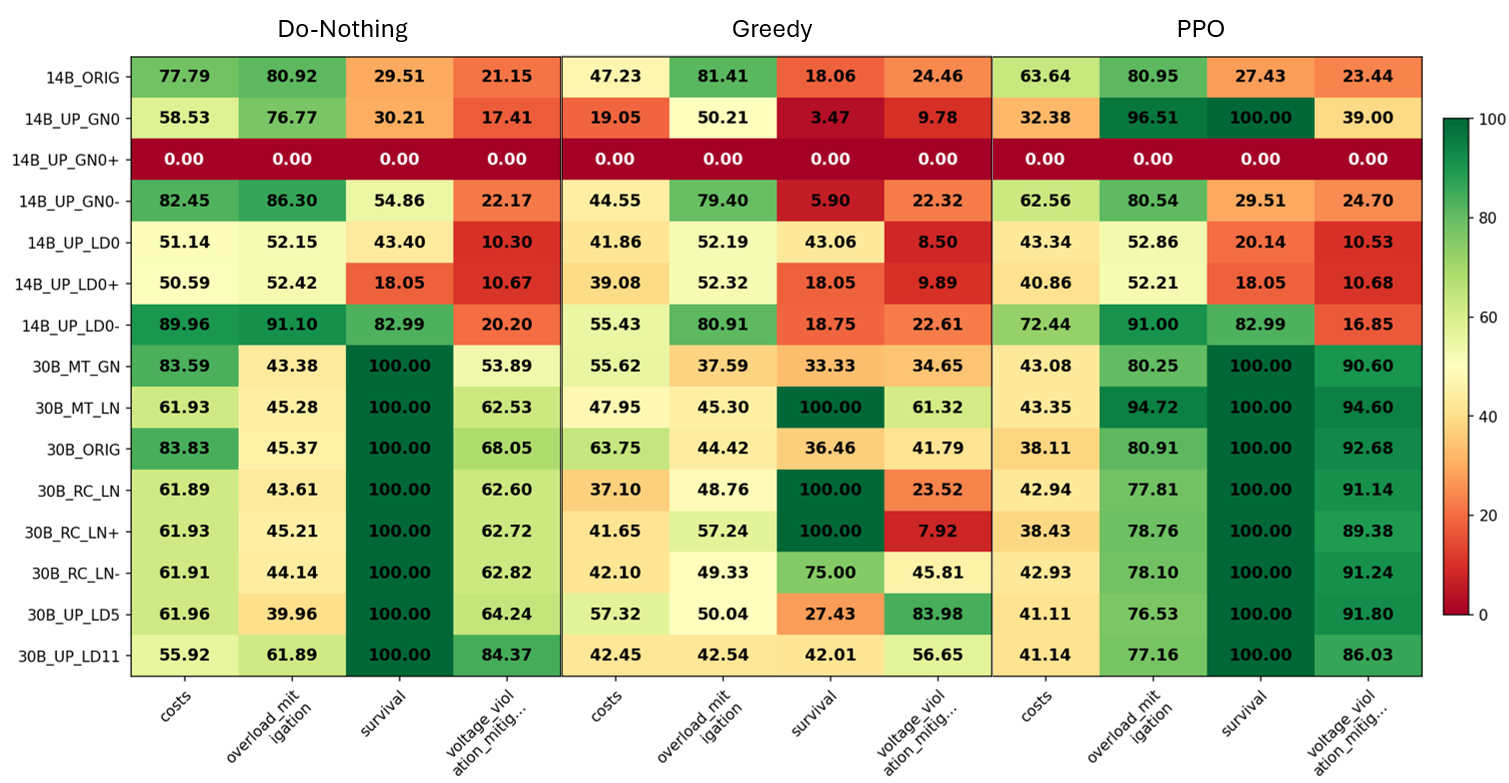
\includegraphics[width=1\textwidth]{images/experiments/heatpmap.png}
    \caption{Category score heatmaps over all experiments for the three evaluated agents}
    \label{fig:exp-heatmap} 
\end{figure}

\FloatBarrier

\subsection{Bus Comparison}
Figure \ref{fig:bus-scores} compares the category scores of the three agents between the 14-bus and 30-bus power grids, highlighting differences in agent performance depending on grid size.

\begin{figure}[htp] % htp = hier (h), top (t), oder auf einer eigenen Seite (p).
    \centering
    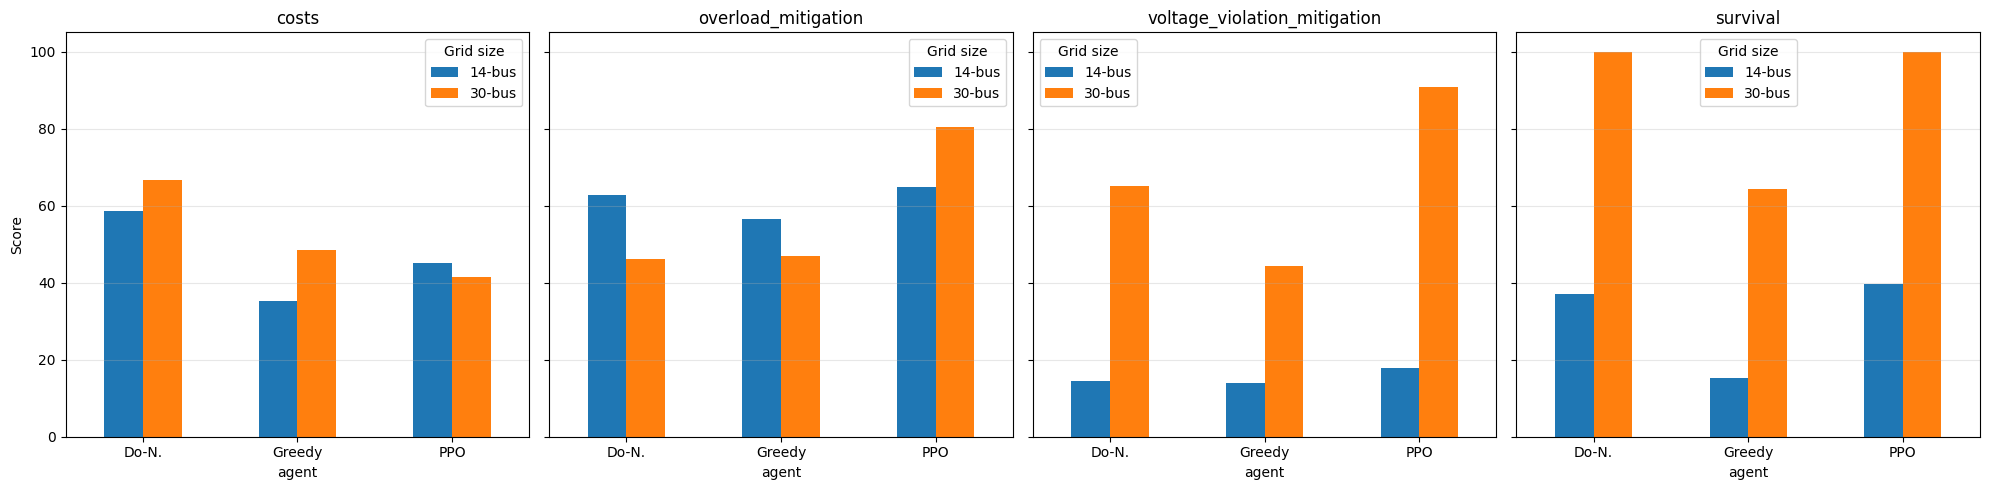
\includegraphics[width=1\textwidth]{images/experiments/bus_scores.png}
    \caption{Category score between the 14- and 30-bus power grids}
    \label{fig:bus-scores} 
\end{figure}


\subsection{Metric Comparison}
Figure \ref{fig:metric-scores} breaks down the category scores of Figure \ref{fig:exp-heatmap} further into their individual metrics, shown separately for the cost, overload mitigation, survival, and voltage violation mitigation categories.

\begin{figure}[htp]
    \centering
    \begin{subfigure}[t]{1\textwidth}
        \centering
        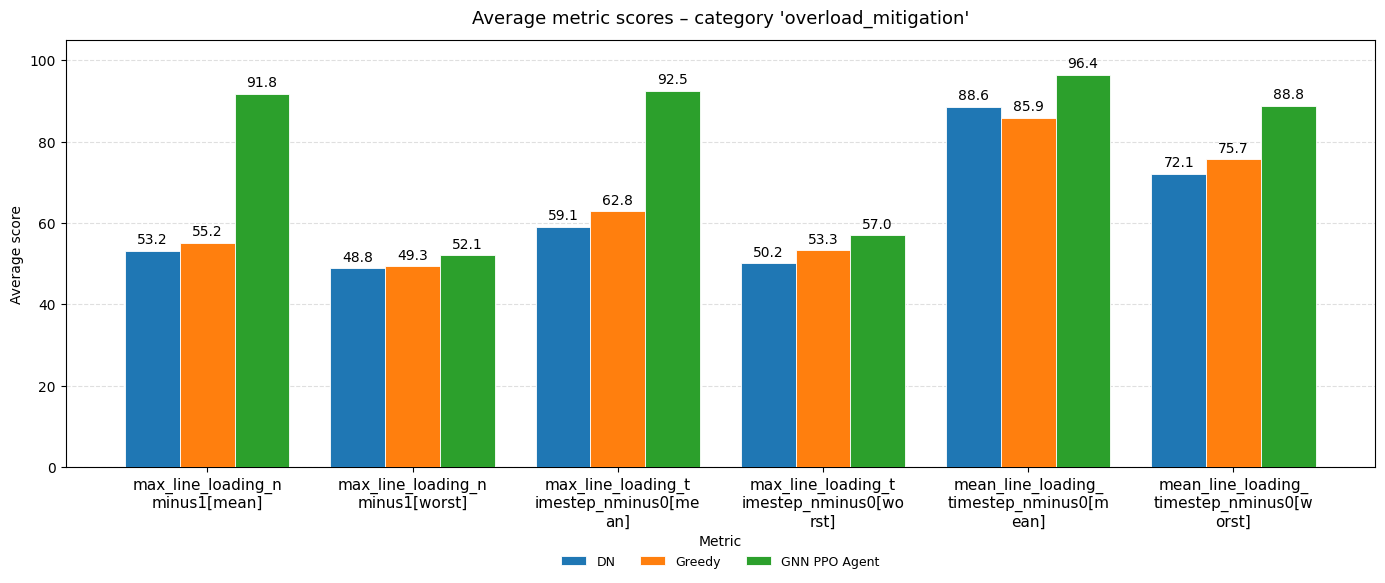
\includegraphics[width=0.9\textwidth]{images/experiments/metric_scores/overload_mitigation1.png}\\[0.1em]
        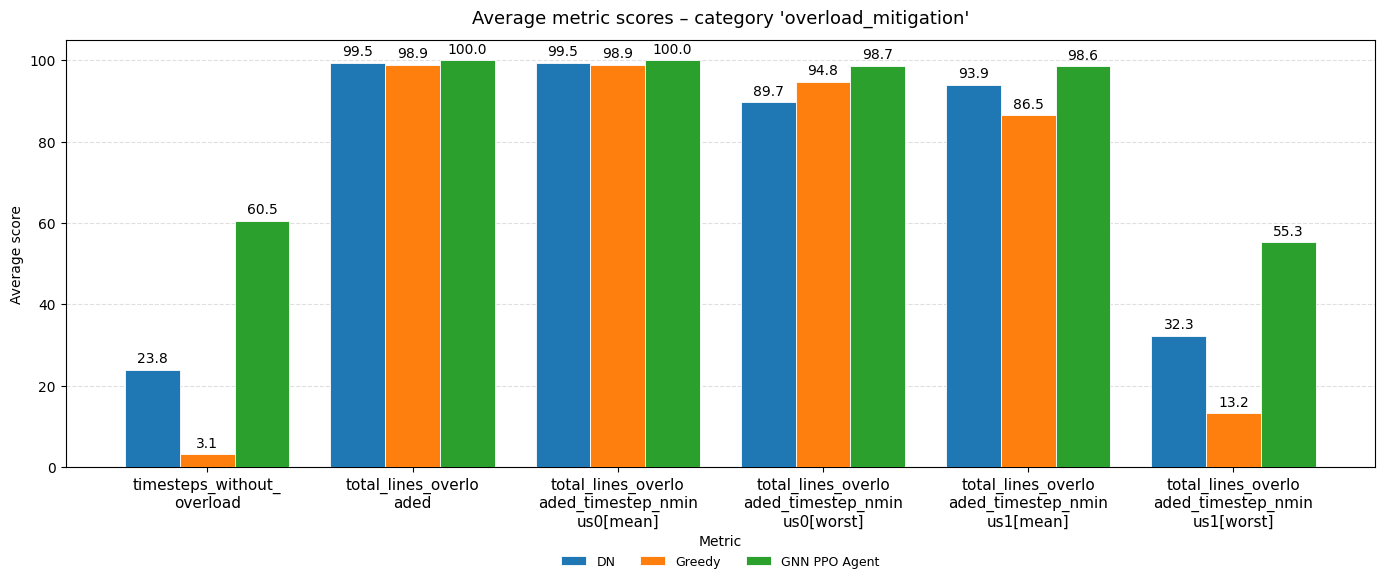
\includegraphics[width=0.9\textwidth]{images/experiments/metric_scores/overload_mitigation2.png}
        \caption{Metric scores over the overload mitigation category for the three evaluated agents}
        \label{fig:metric-scores-overload} 
    \end{subfigure}
    \caption{Metric scores over different categories for all three evaluated agents}
    \label{fig:metric-scores}
\end{figure}

\begin{figure}[htp]
    \ContinuedFloat
    \centering

    \begin{subfigure}[t]{1\textwidth}
        \centering
        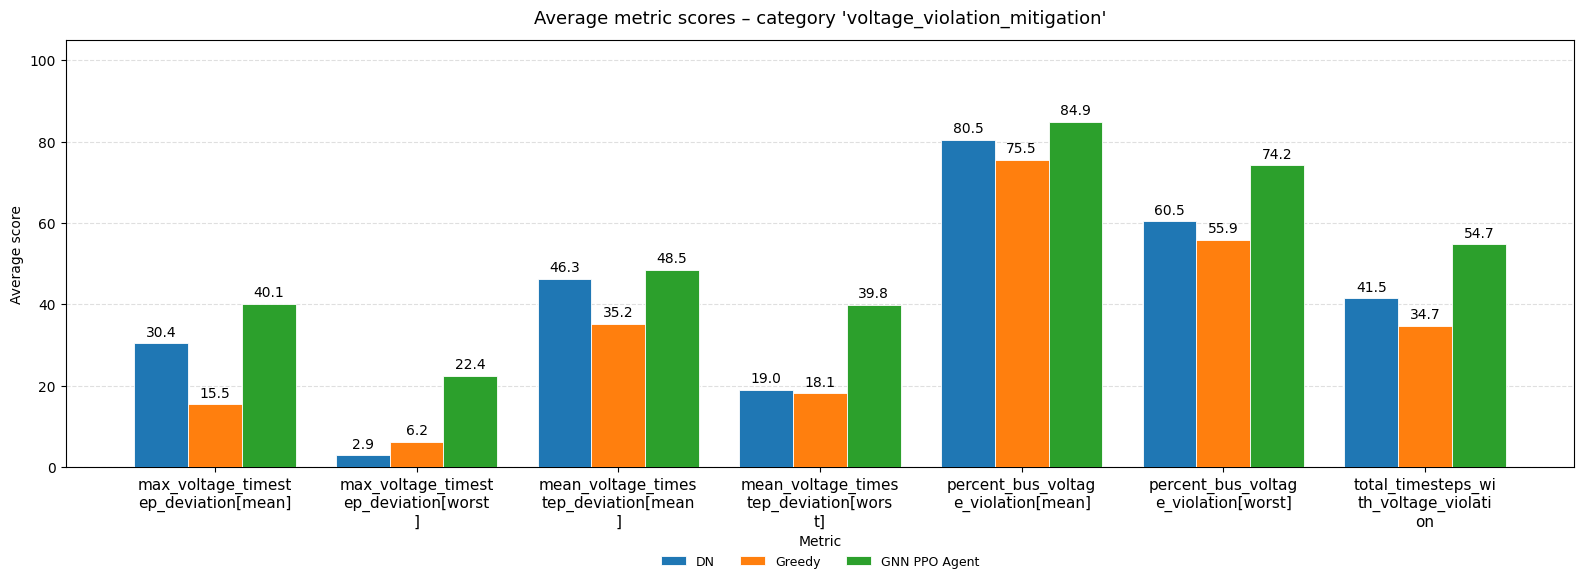
\includegraphics[width=\textwidth]{images/experiments/metric_scores/voltage_violation_mitigation.png}
        \caption{Metric scores over the voltage violation mitigation category for the three evaluated agents}
        \label{fig:metric-scores-voltage-violation} 
    \end{subfigure}

    \vspace{0.2em}

    \begin{subfigure}[t]{1\textwidth}
        \centering
        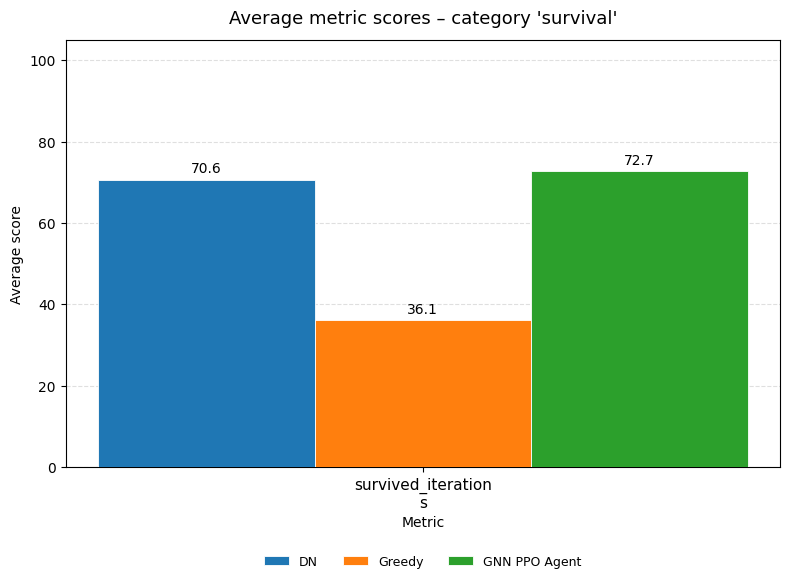
\includegraphics[width=0.55\textwidth]{images/experiments/metric_scores/survival.png}
        \caption{Metric scores over the survival category for the three evaluated agents}
        \label{fig:metric-scores-survival} 
    \end{subfigure}

    \vspace{0.2em}

    \begin{subfigure}[t]{1\textwidth}
        \centering
        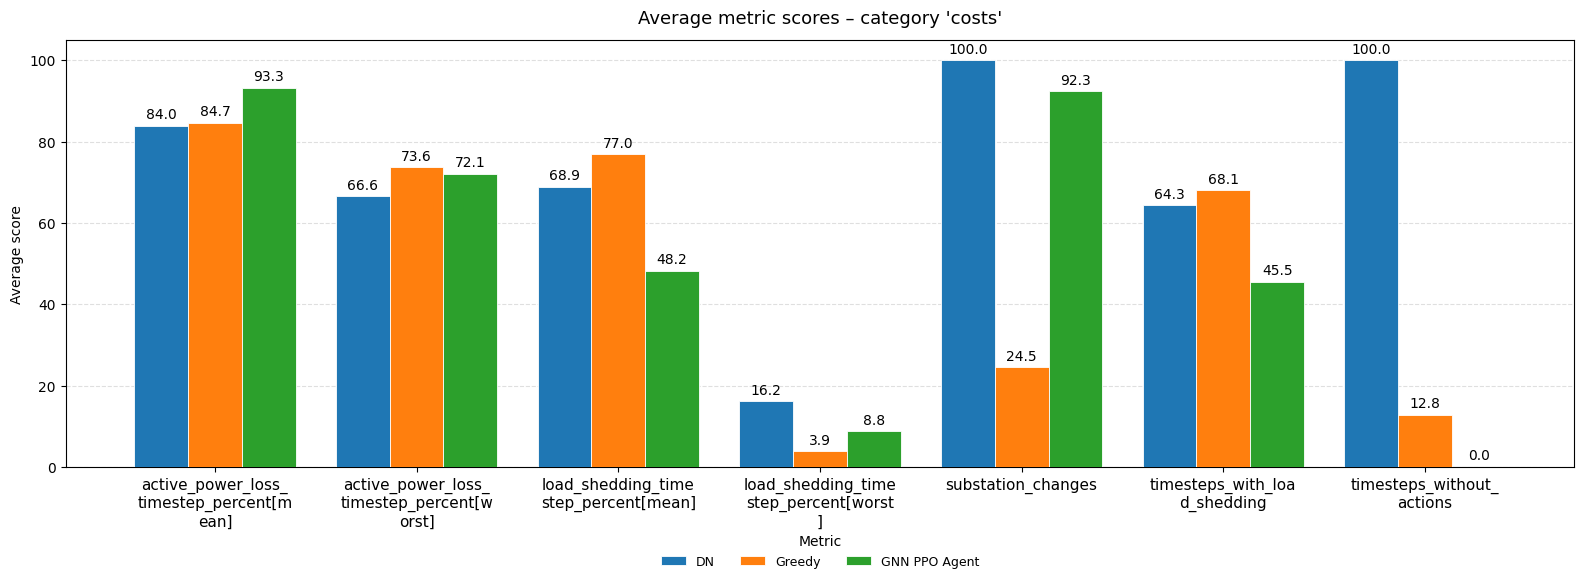
\includegraphics[width=\textwidth]{images/experiments/metric_scores/costs.png}
        \caption{Metric scores over the cost category for the three evaluated agents}
        \label{fig:metric-scores-costs} 
    \end{subfigure}

    \caption{Metric scores over different categories for all three evaluated agents (continued)}
\end{figure}

\FloatBarrier







\section{Stress Test}\label{sec:exp-stress-test}
Figures \ref{fig:tot-score-gen-stress}, \ref{fig:tot-score-load-stress}, and \ref{fig:tot-score-line-cap-stress} show the total score distributions achieved by the three agents across the increasing stress levels of the generator, load, and line capacity stress test experiments, respectively.

\begin{figure}[htp] % htp = hier (h), top (t), oder auf einer eigenen Seite (p).
    \centering
    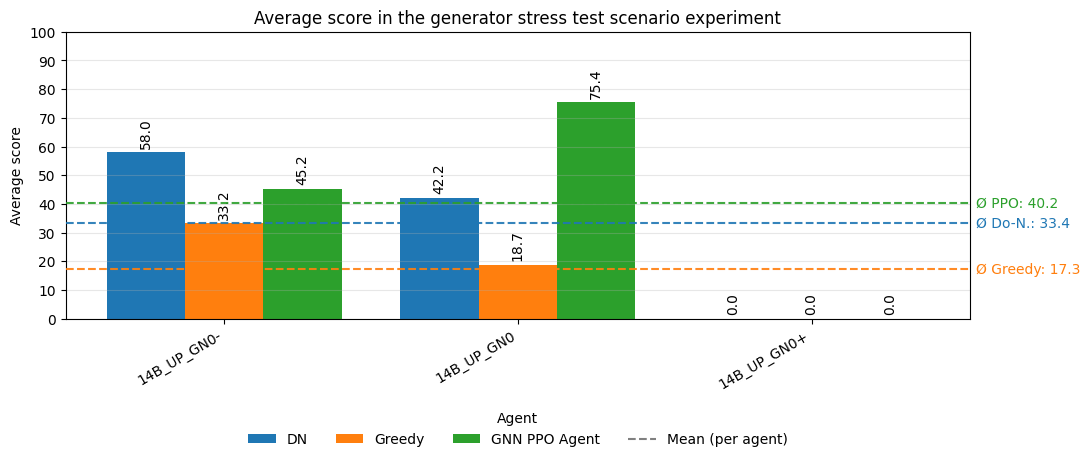
\includegraphics[width=0.87\textwidth]{images/experiments/total_scores/gen_stress.png}
    \caption{Total score overview for the generator stress test experiment, with average values of each agent}
    \label{fig:tot-score-gen-stress} 
\end{figure}


\begin{figure}[htp] % htp = hier (h), top (t), oder auf einer eigenen Seite (p).
    \centering
    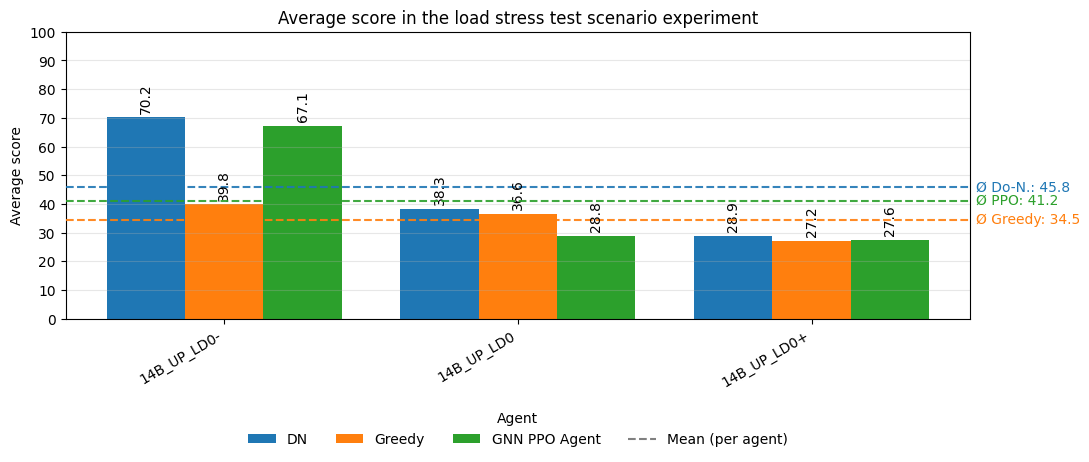
\includegraphics[width=0.87\textwidth]{images/experiments/total_scores/load_stress.png}
    \caption{Total score overview for the load stress test experiment, with average values of each agent}
    \label{fig:tot-score-load-stress} 
\end{figure}


\begin{figure}[htp] % htp = hier (h), top (t), oder auf einer eigenen Seite (p).
    \centering
    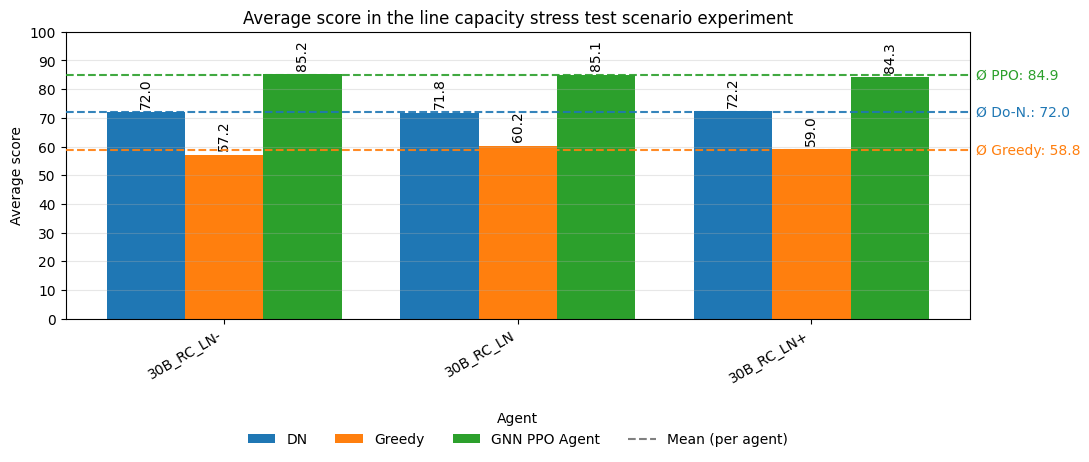
\includegraphics[width=0.87\textwidth]{images/experiments/total_scores/line_cap_stress.png}
    \caption{Total score overview for the line capacity stress test experiment, with average values of each agent}
    \label{fig:tot-score-line-cap-stress} 
\end{figure}

\FloatBarrier





\section{Single Scenario Comparison}\label{sec:exp-single-scenario}
This section provides a detailed, run-level breakdown of the category scores for every scenario evaluated in the standard, diverse and stress test experiments, complementing the aggregated results shown in Sections \ref{sec:exp-general-overview} and \ref{sec:exp-stress-test}.

\subsection{Standard Test Scenarios}
Figure \ref{fig:scenario-scores-orig} shows the category scores achieved by the three agents on the two unmodified base grids.

\begin{figure}[htp]
    \centering
    \begin{subfigure}[t]{1\textwidth}
        \centering
        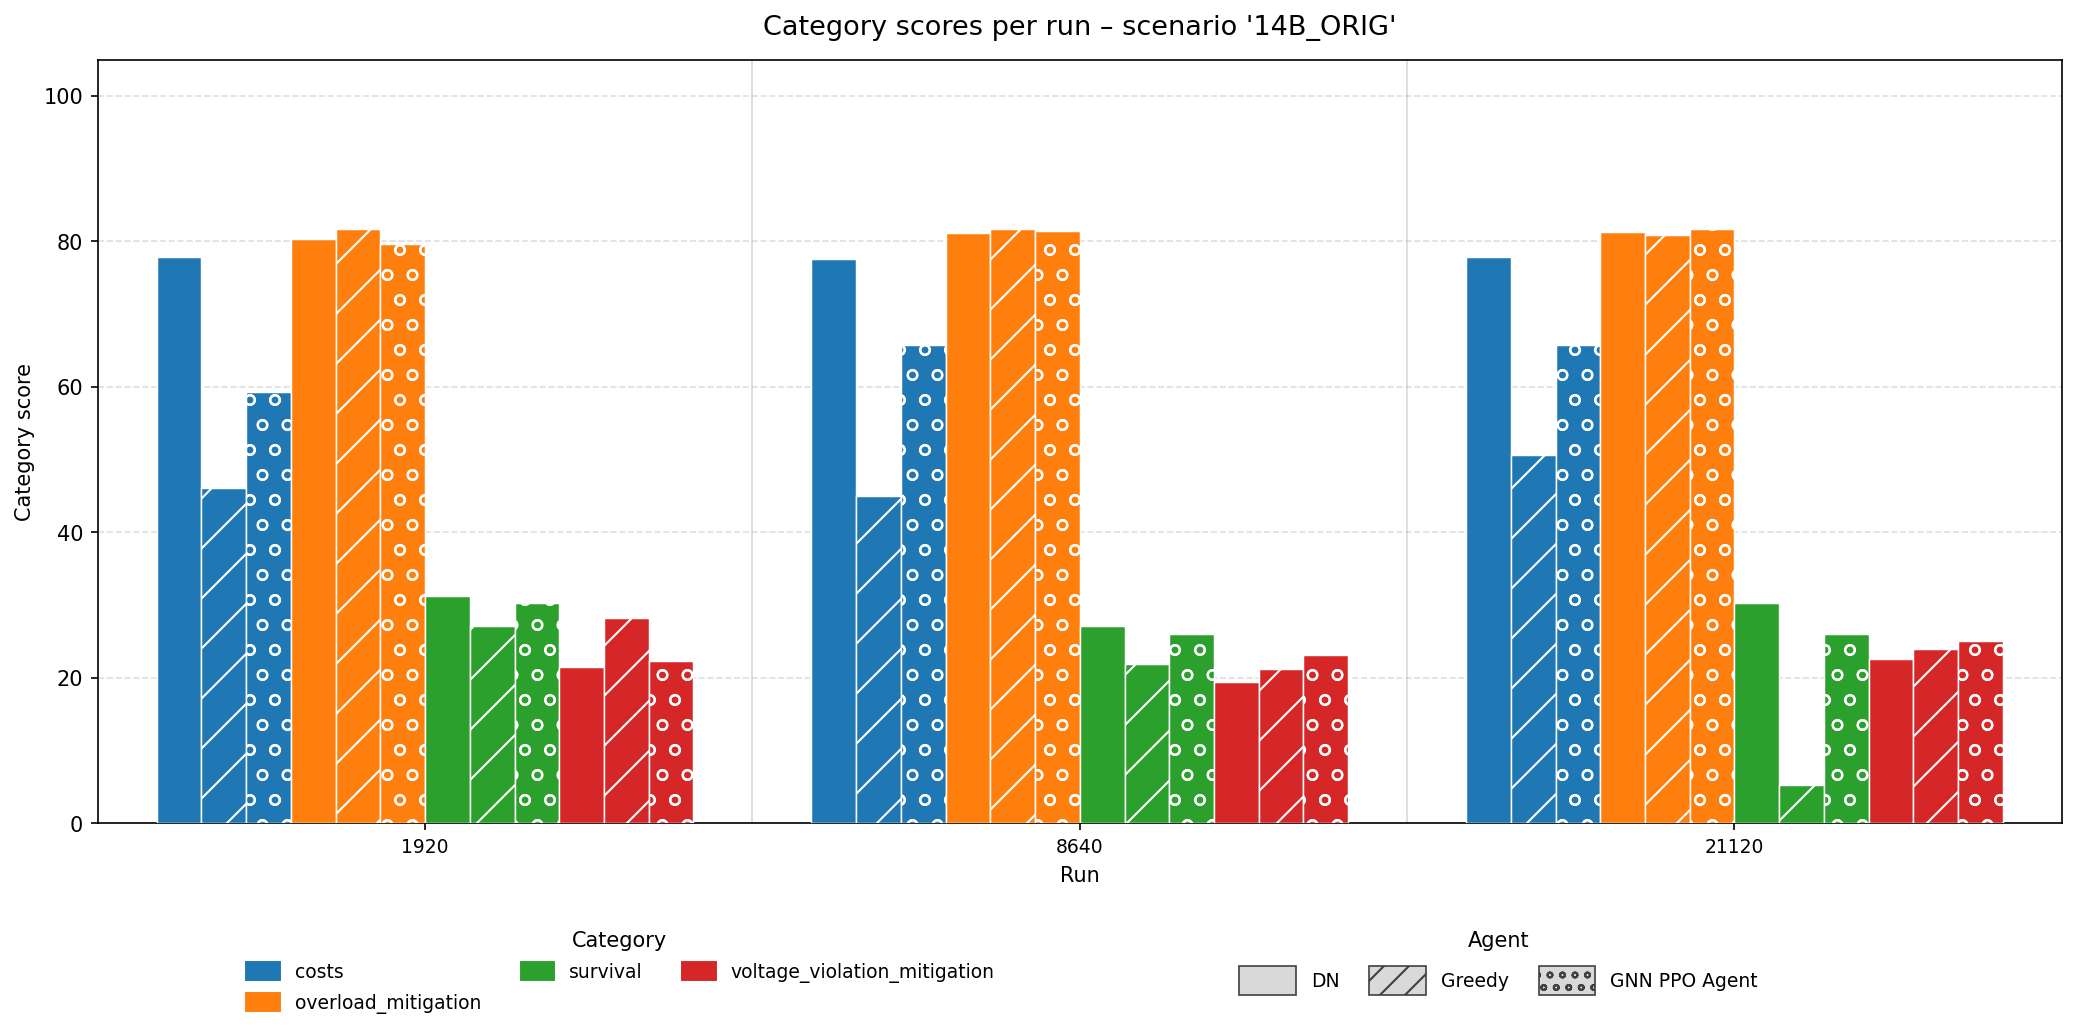
\includegraphics[width=\textwidth]{images/experiments/scenario_scores/14B_ORIG.png}
        \caption{14-bus unmodified power grid}
        \label{fig:scenario-scores-14b-orig}
    \end{subfigure}

    \vspace{0.2em}

    \begin{subfigure}[t]{0.65\textwidth}
        \centering
        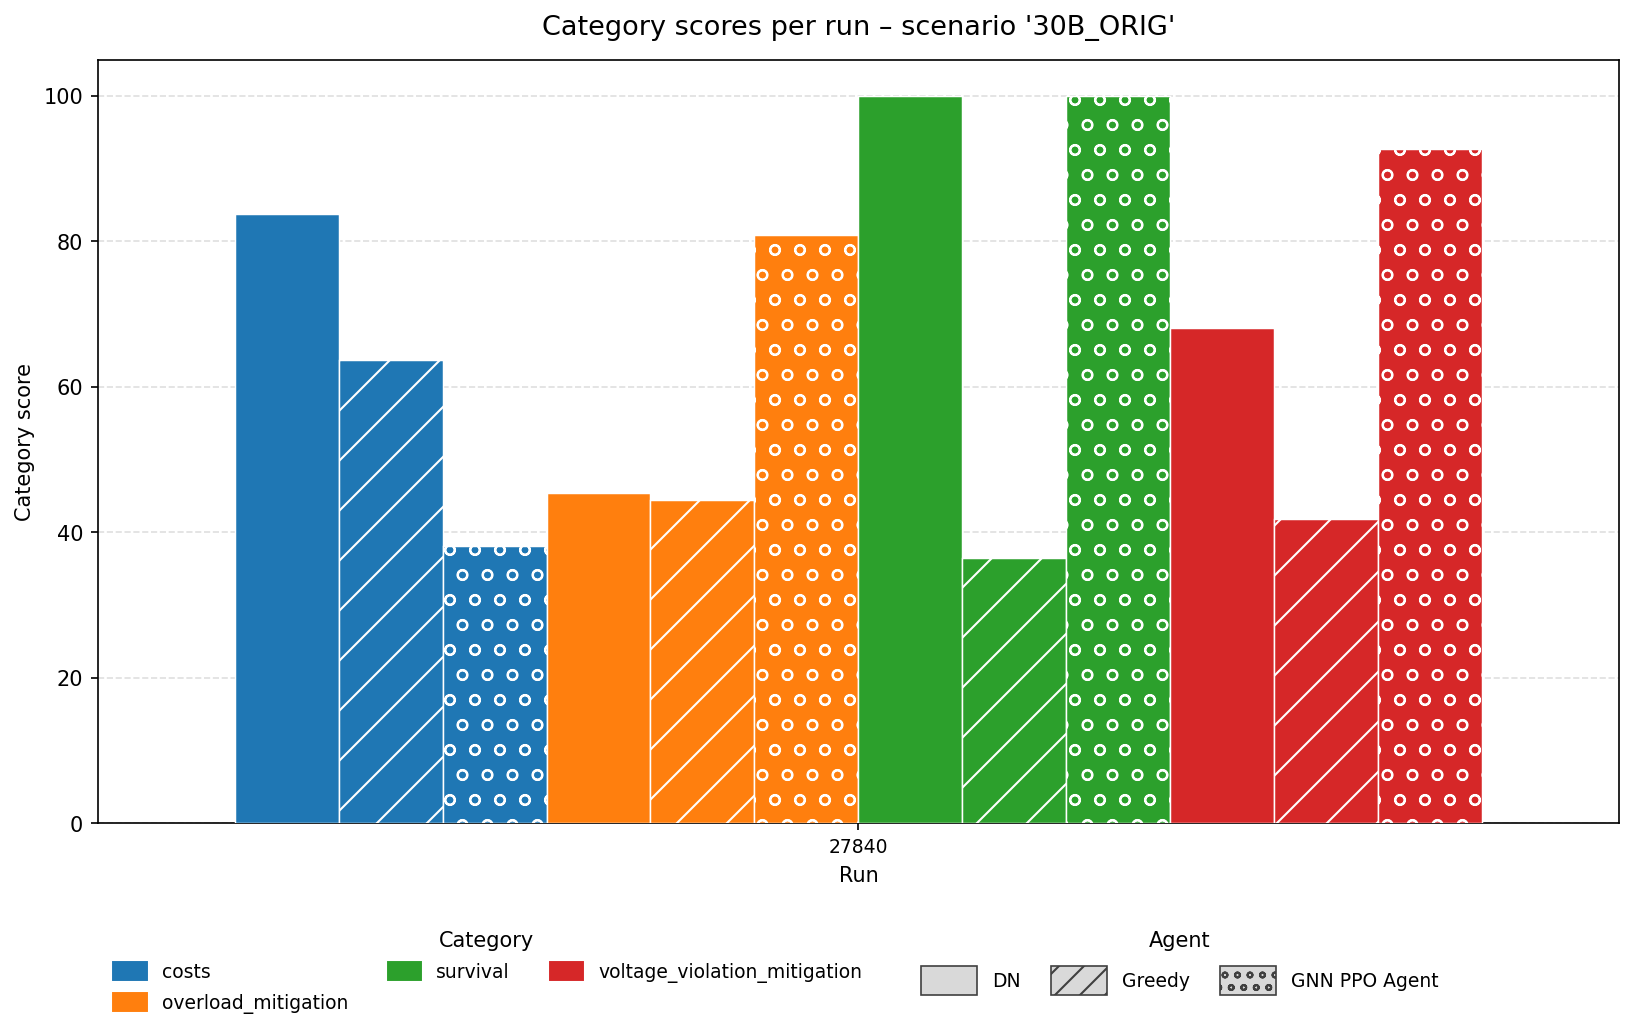
\includegraphics[width=\textwidth]{images/experiments/scenario_scores/30B_ORIG.png}
        \caption{30-bus unmodified power grid}
        \label{fig:scenario-scores-30b-orig}
    \end{subfigure}

    \caption{Score overview over the standard test runs}
    \label{fig:scenario-scores-orig}
\end{figure}

\FloatBarrier

\subsection{Diverse Scenarios}
Figures \ref{fig:scenario-scores-14b-gnld-scaled} to \ref{fig:scenario-scores-rc} show the category scores achieved by the three agents on the diverse scenarios, in which either a generator or load was scaled, a maintenance event was triggered, or the thermal line capacity was reduced.

\begin{figure}[htp]
    \centering

    \begin{subfigure}[t]{1\textwidth}
        \centering
        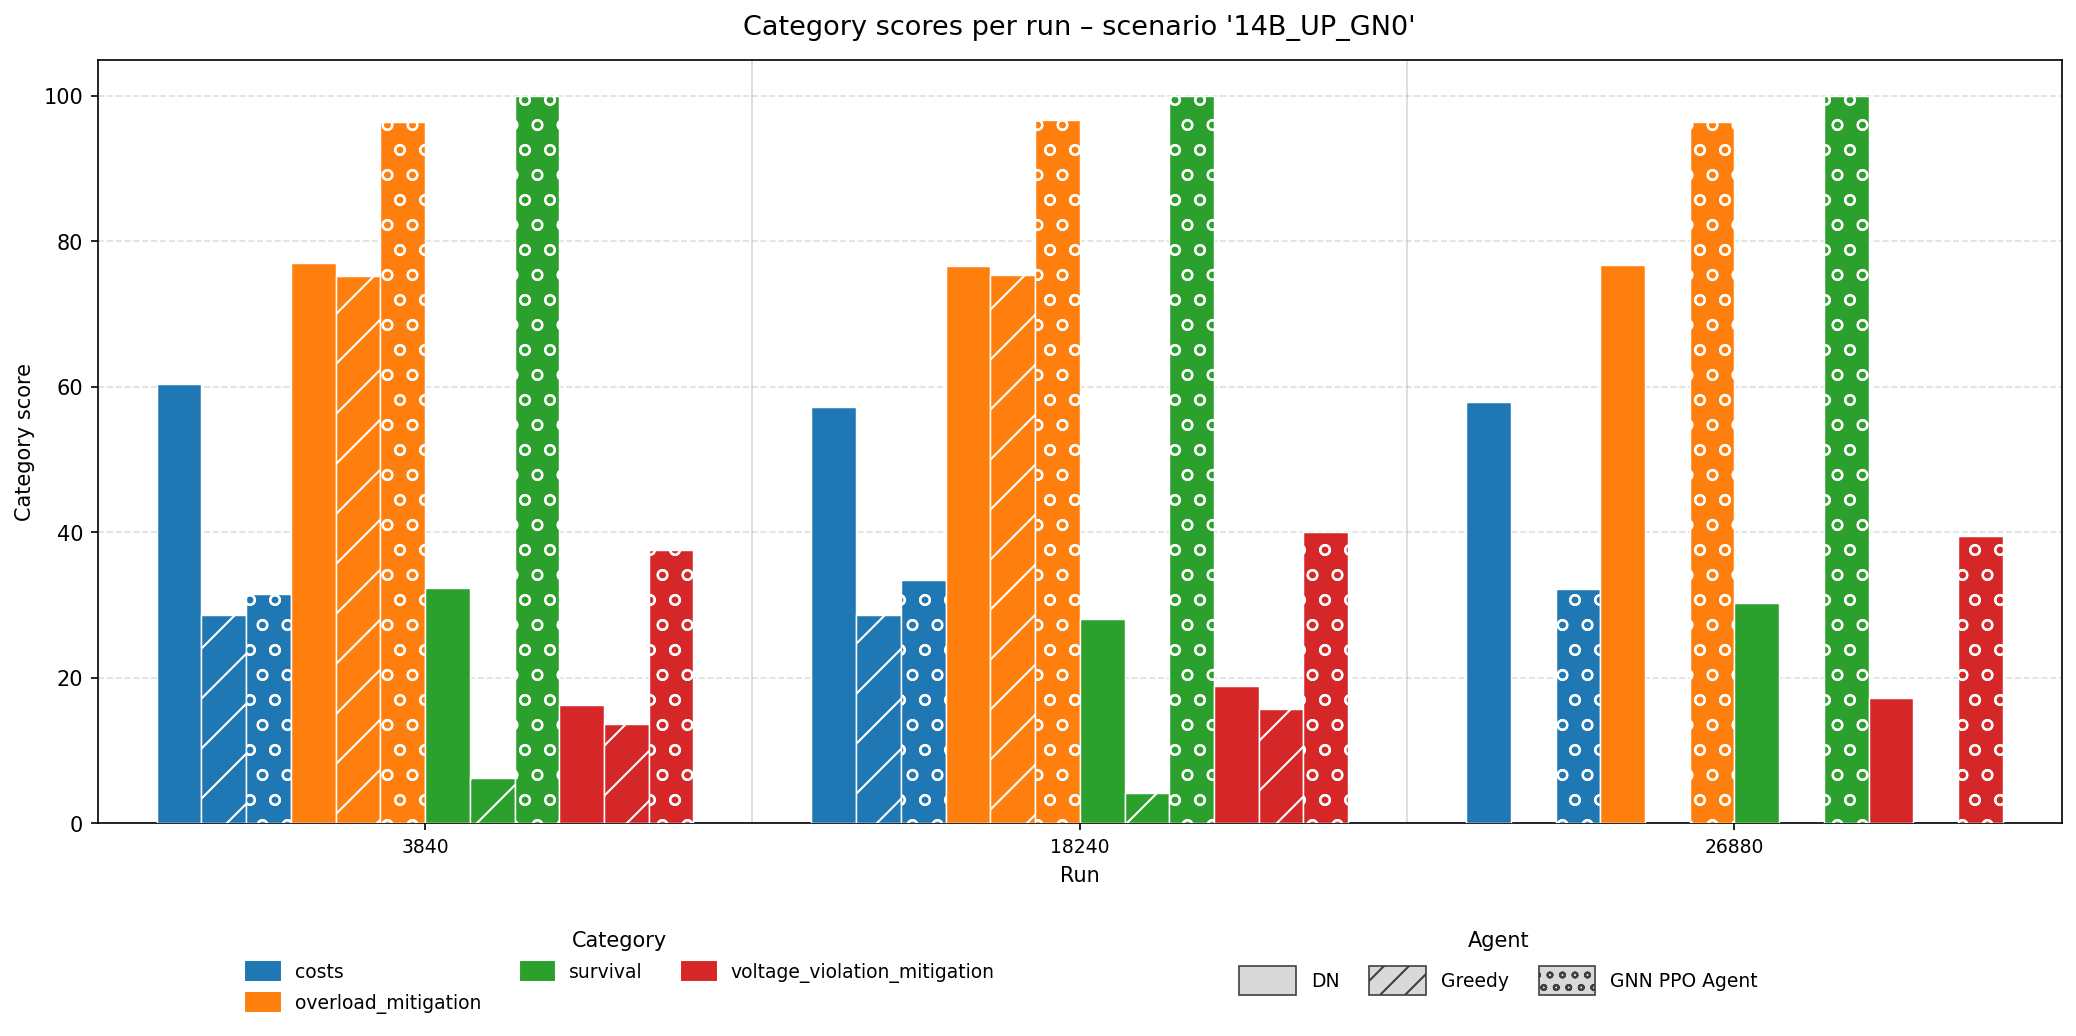
\includegraphics[width=\textwidth]{images/experiments/scenario_scores/14B_UP_GN0.png}
        \caption{14-bus with increased power generation in generator 0}
        \label{fig:scenario-scores-14b-up-gn0} 
    \end{subfigure}

    \vspace{0.2em}

    \begin{subfigure}[t]{0.65\textwidth}
        \centering
        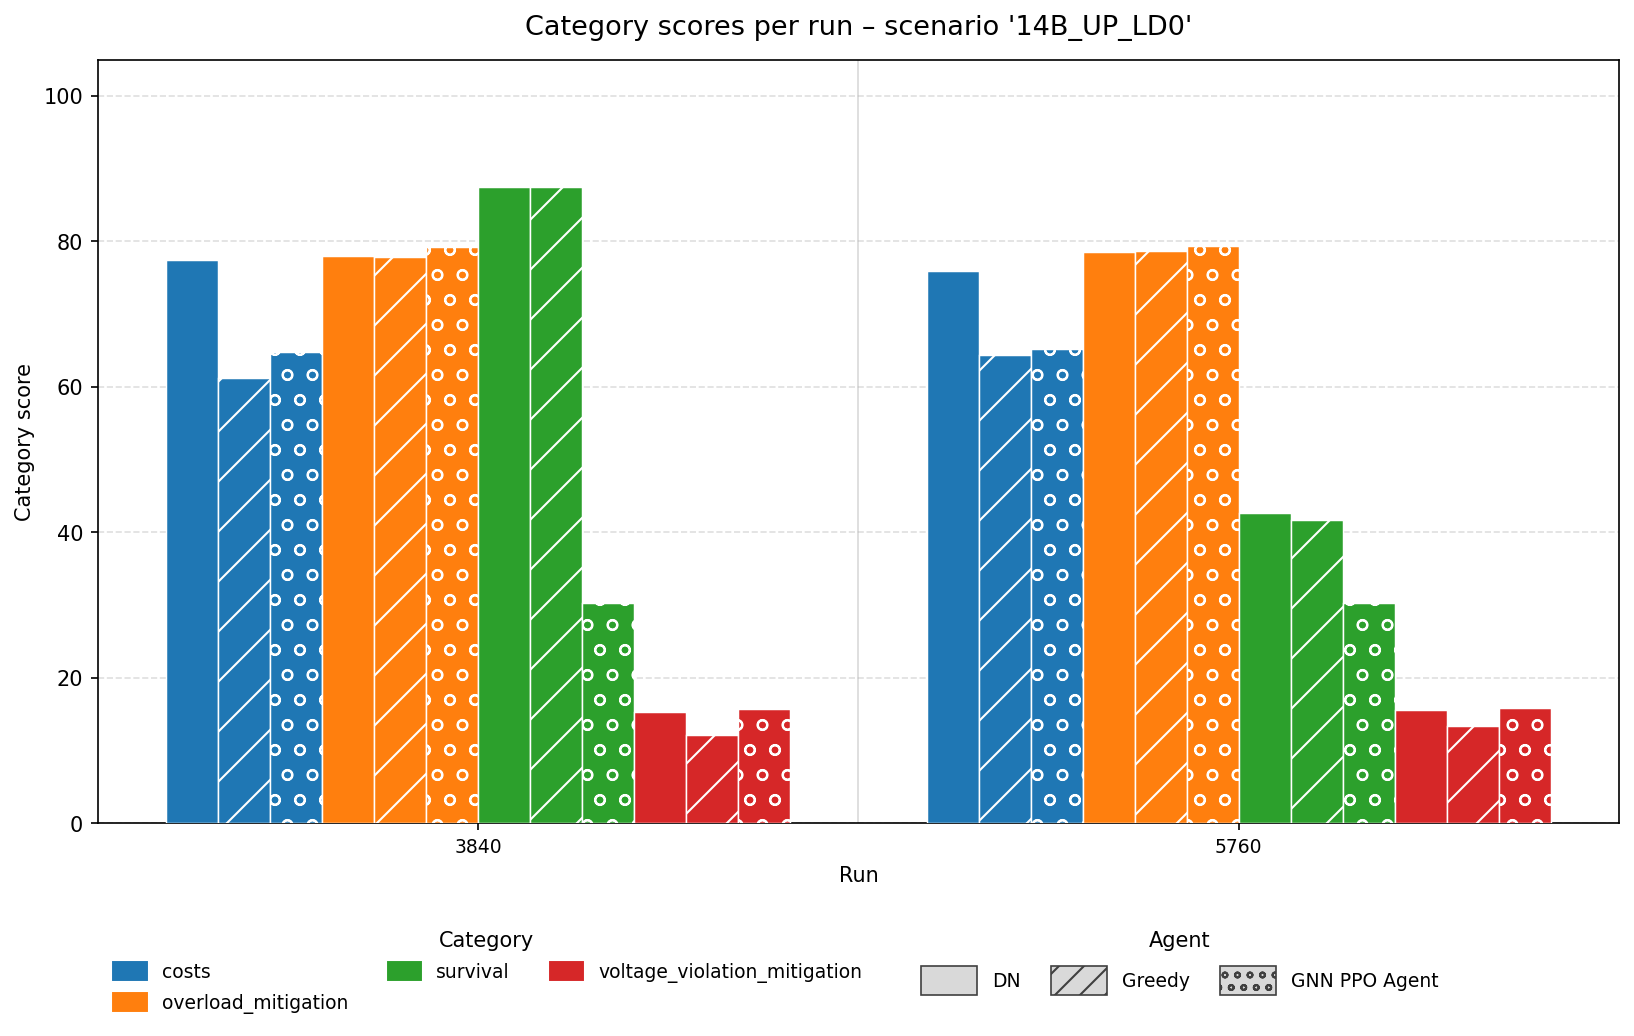
\includegraphics[width=\textwidth]{images/experiments/scenario_scores/14B_UP_LD0.png}
        \caption{14-bus with increased power consumption in load 0}
        \label{fig:scenario-scores-14b-up-ld0}
    \end{subfigure}

    \caption{Score overview over the scenarios in the 14-bus grid in which a generator or load was modified}
    \label{fig:scenario-scores-14b-gnld-scaled}
\end{figure}

\begin{figure}[htp]
    \centering

    \begin{subfigure}[t]{1\textwidth}
        \centering
        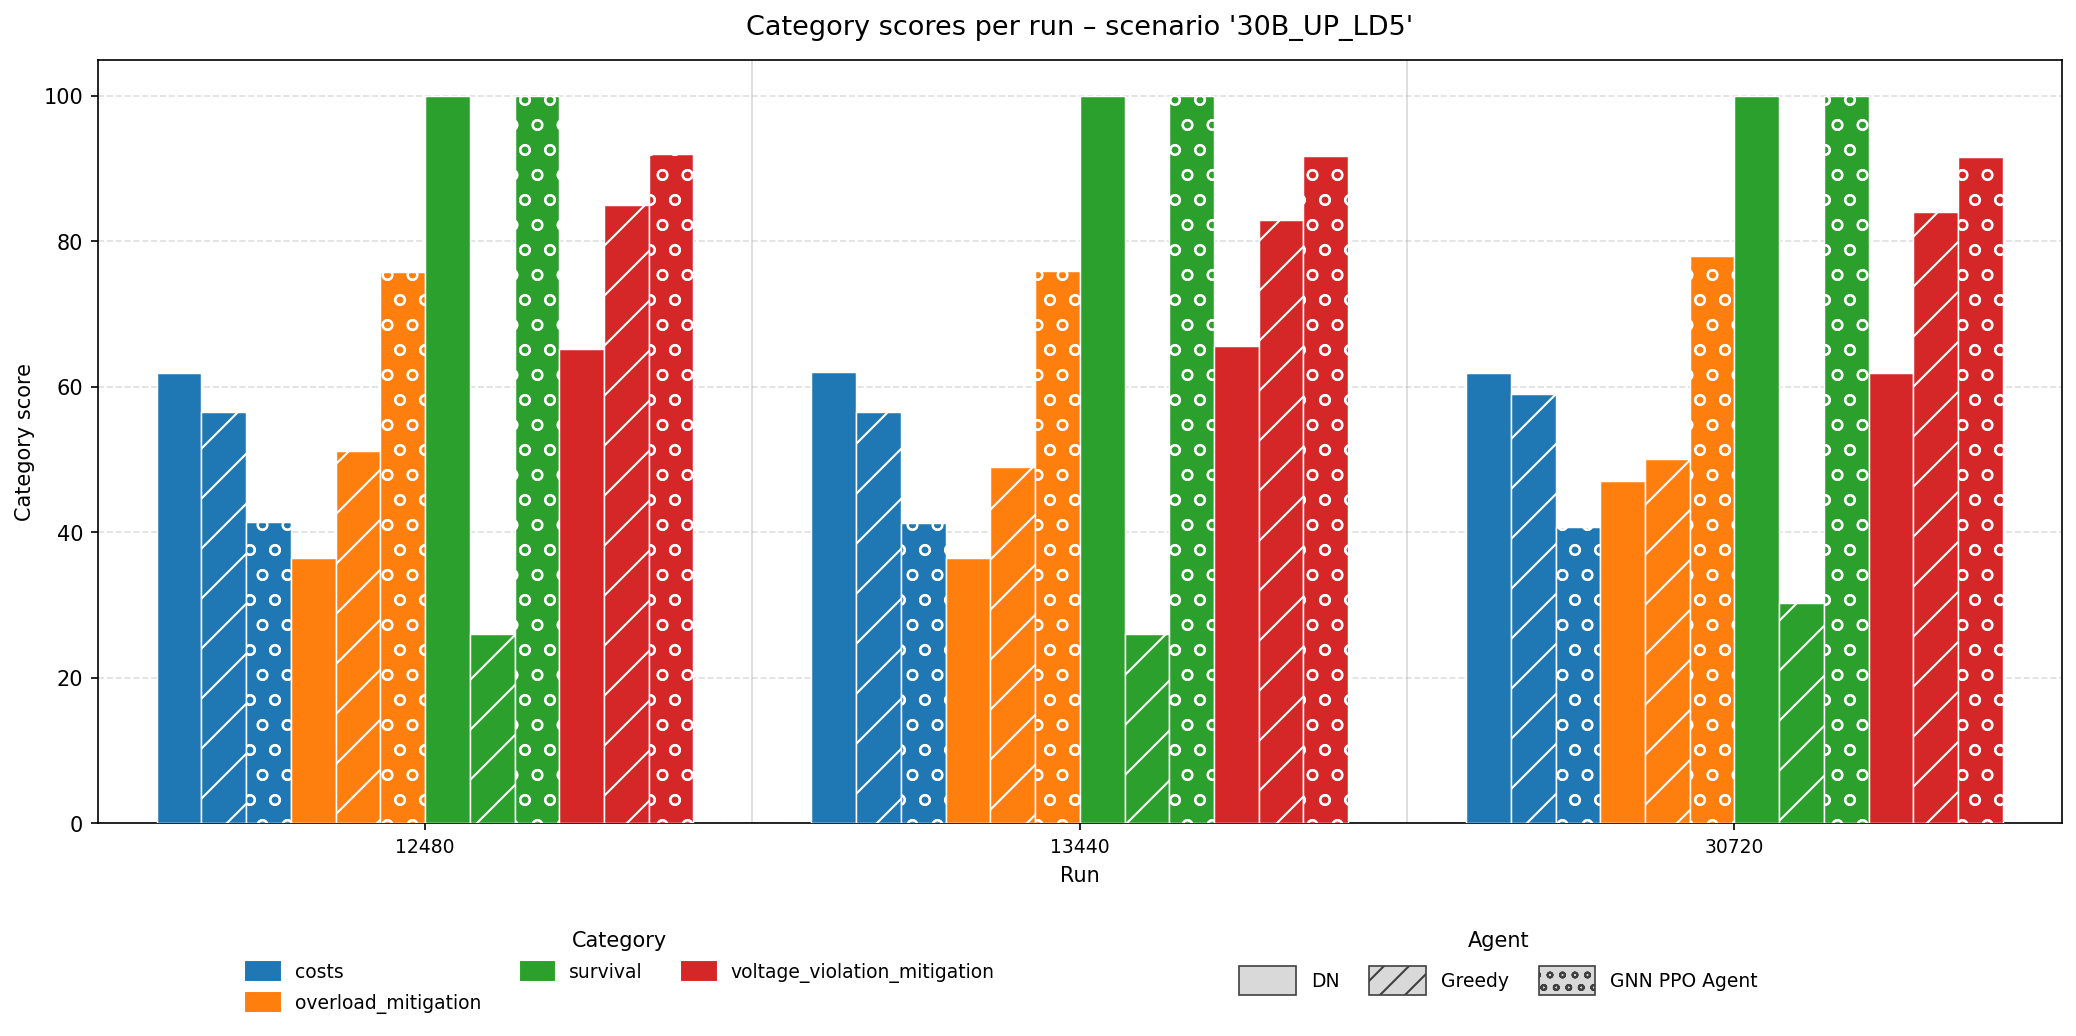
\includegraphics[width=0.93\textwidth]{images/experiments/scenario_scores/30B_UP_LD5.png}
        \caption{30-bus with increased power consumption in load 5}
        \label{fig:scenario-scores-30b-up-ld5}
    \end{subfigure}

    \vspace{0.2em}

    \begin{subfigure}[t]{1\textwidth}
        \centering
        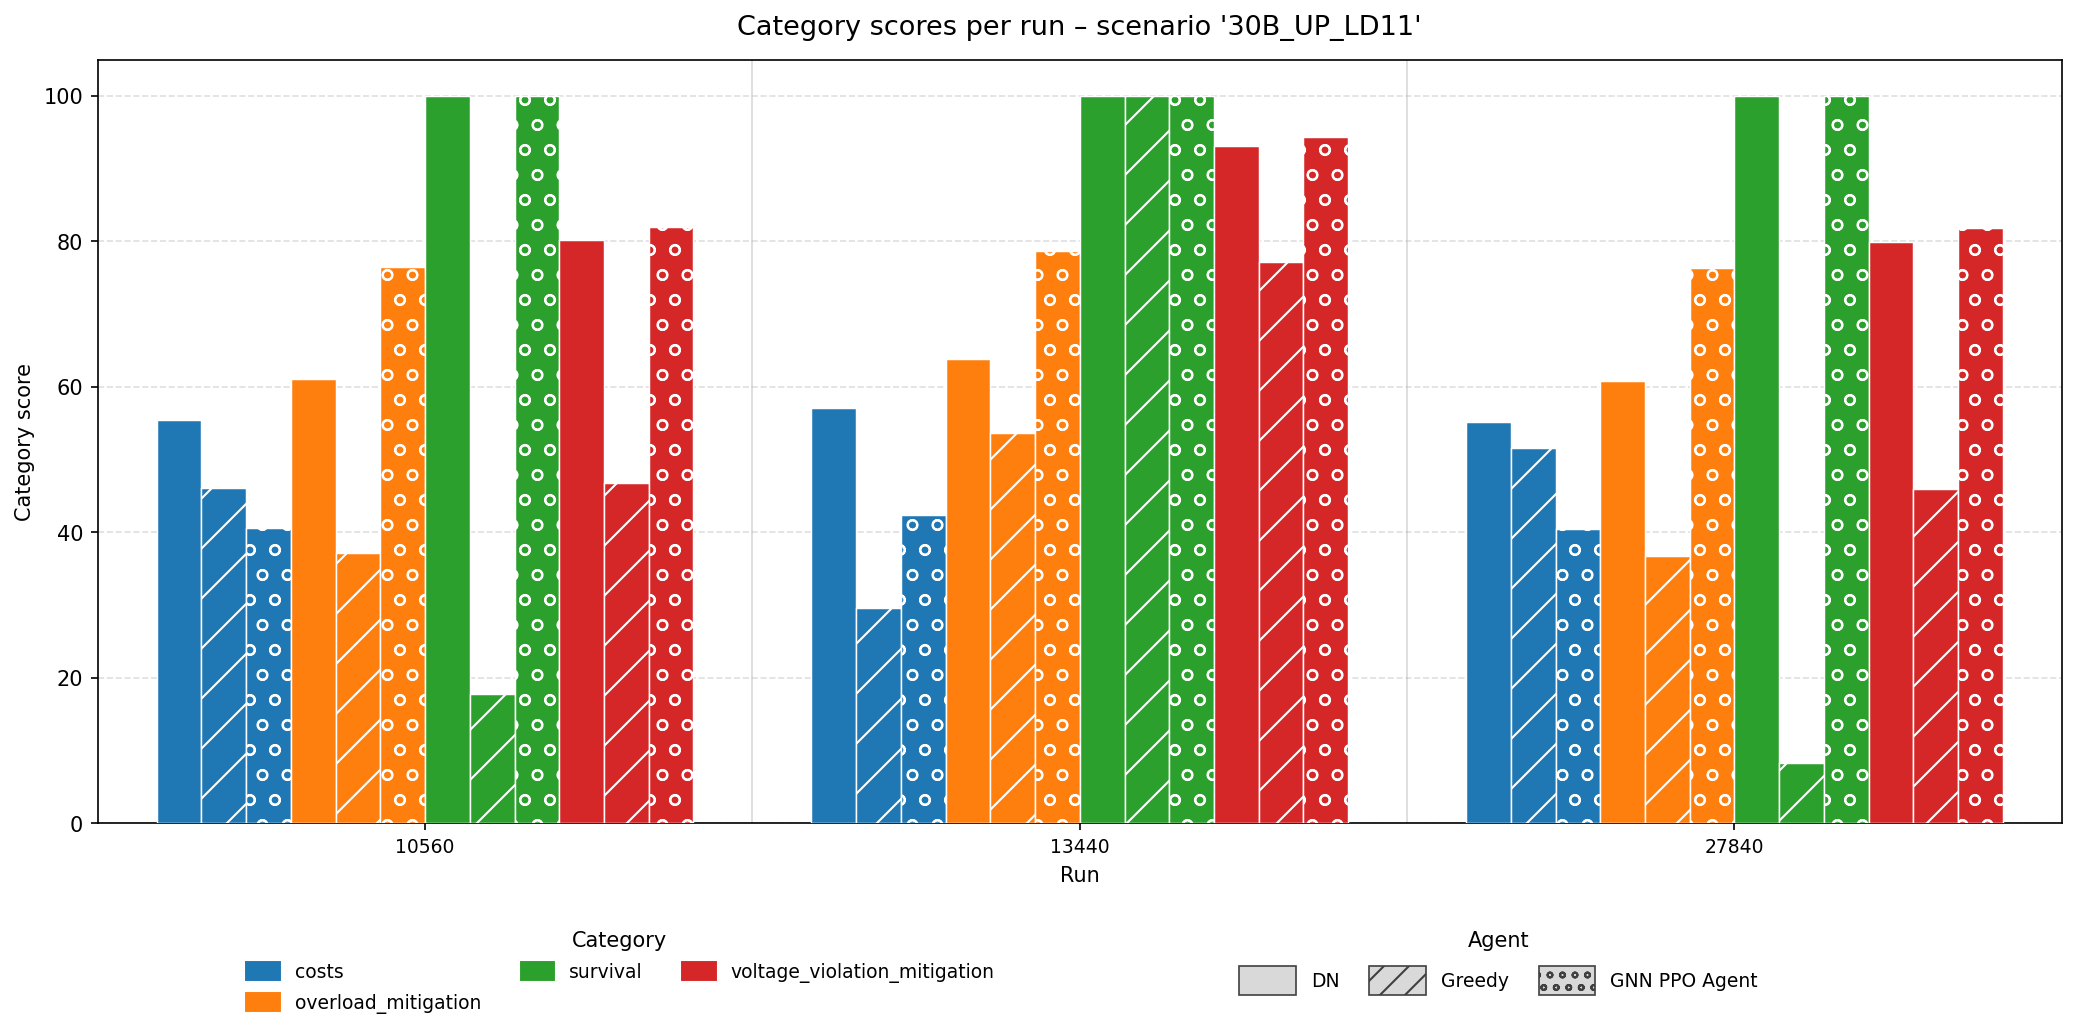
\includegraphics[width=0.93\textwidth]{images/experiments/scenario_scores/30B_UP_LD11.png}
        \caption{30-bus with increased power consumption in load 11}
        \label{fig:scenario-scores-30b-up-ld11}
    \end{subfigure}

    \caption{Score overview over the scenarios in the 30-bus grid where loads were modified}
    \label{fig:scenario-scores-30b-ld-scaled}
\end{figure}

\begin{figure}[htp]
    \centering
    \begin{subfigure}[t]{0.65\textwidth}
        \centering
        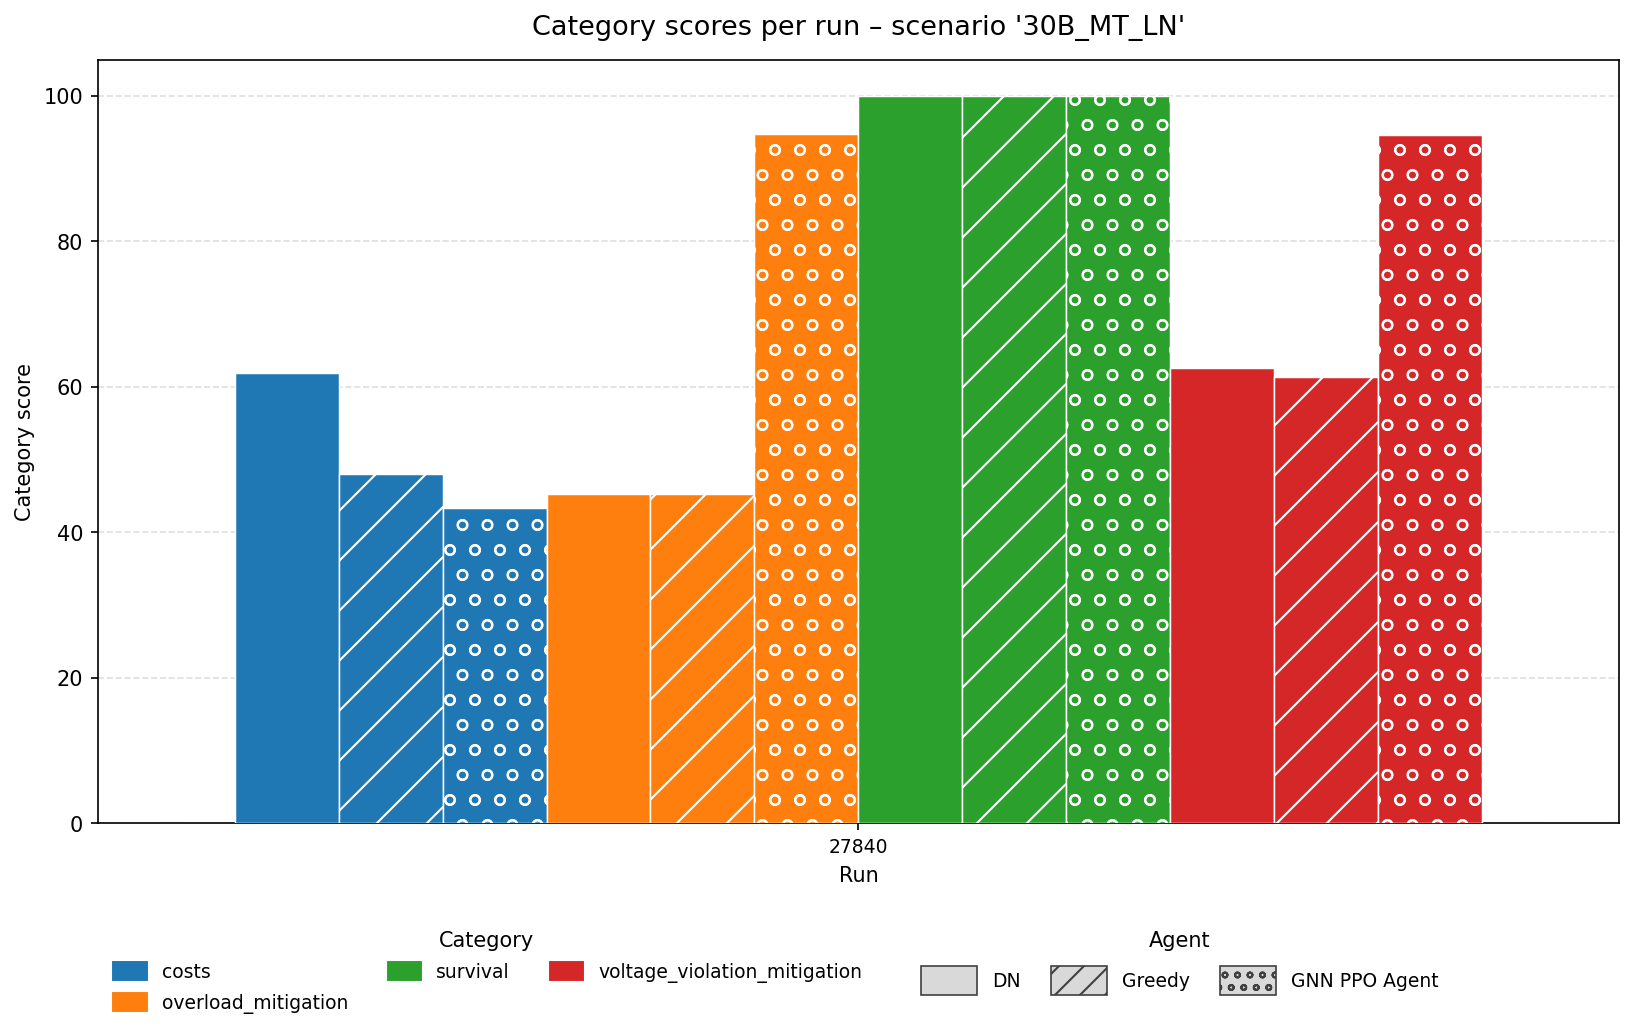
\includegraphics[width=\textwidth]{images/experiments/scenario_scores/30B_MT_LN.png}
        \caption{30-bus with maintenance in lines}
        \label{fig:scenario-scores-30b-mt-ln}
    \end{subfigure}
    \caption{Score overview over the scenarios where lines or generators had a maintenance event}
    \label{fig:scenario-scores-mnt}
\end{figure}

\begin{figure}[htp]\ContinuedFloat
    \centering
    \begin{subfigure}[t]{0.65\textwidth}
        \centering
        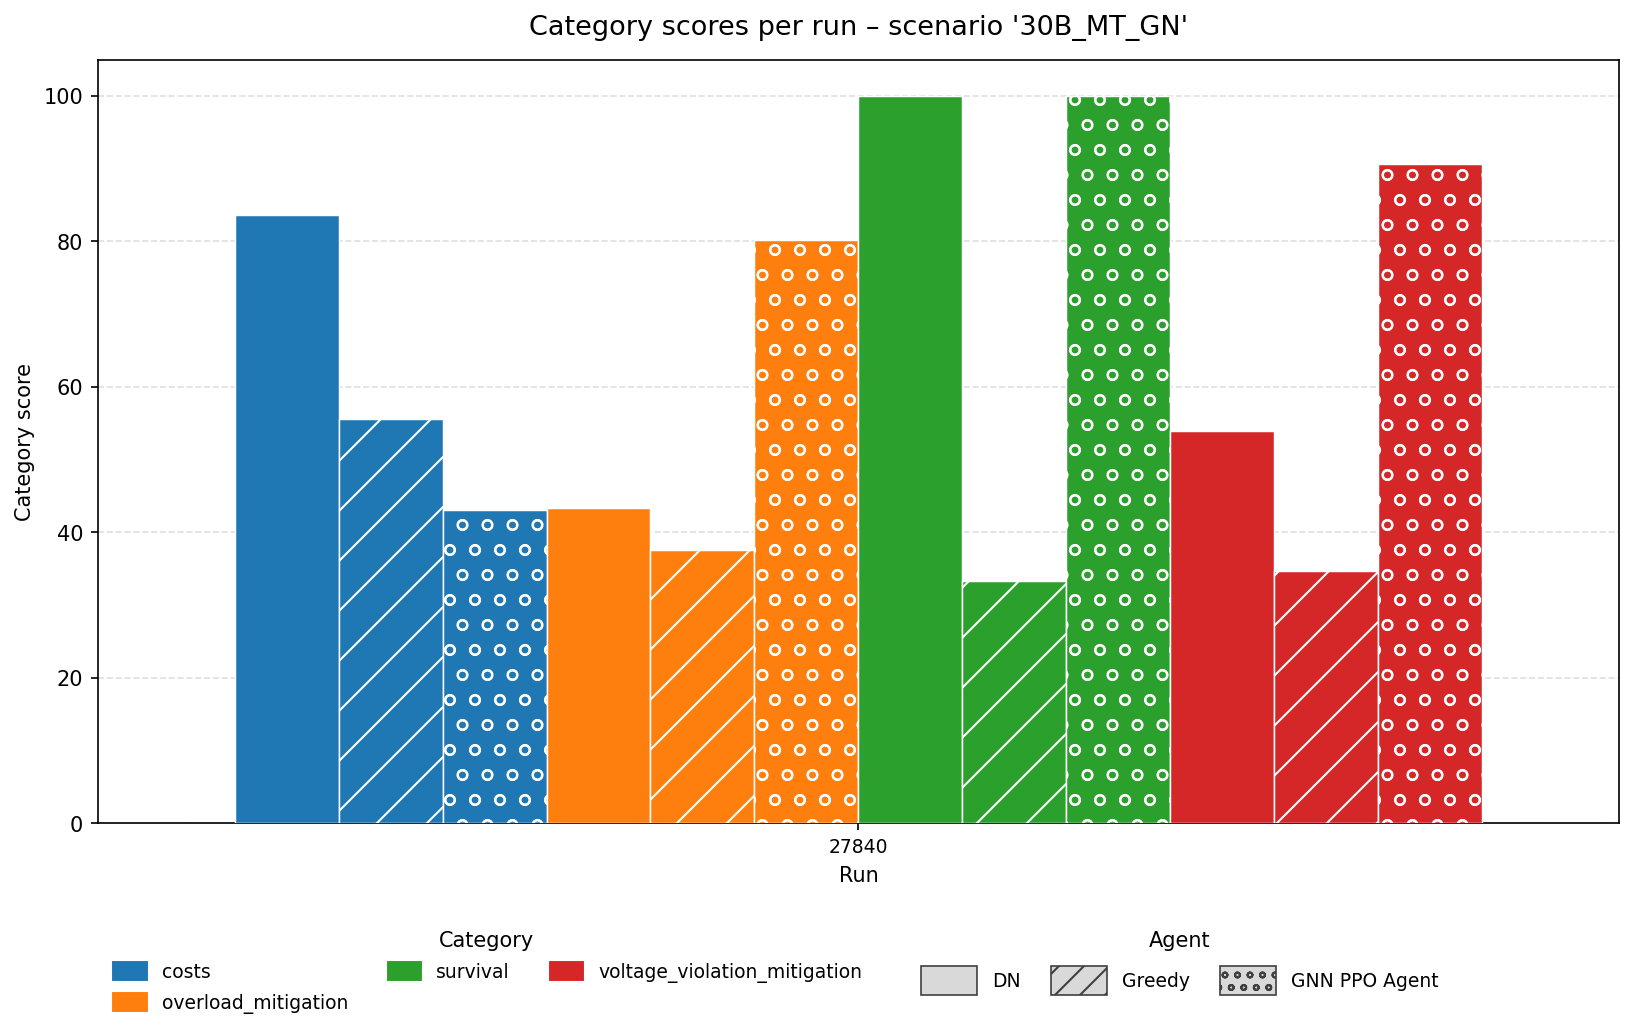
\includegraphics[width=\textwidth]{images/experiments/scenario_scores/30B_MT_GN.png}
        \caption{30-bus with maintenance in one generator}
        \label{fig:scenario-scores-30b-mt-gn}
    \end{subfigure}
    \caption{Score overview over the scenarios where lines or generators had a maintenance event (continued)}
\end{figure}

\begin{figure}[htp] % htp = hier (h), top (t), oder auf einer eigenen Seite (p).
    \centering
    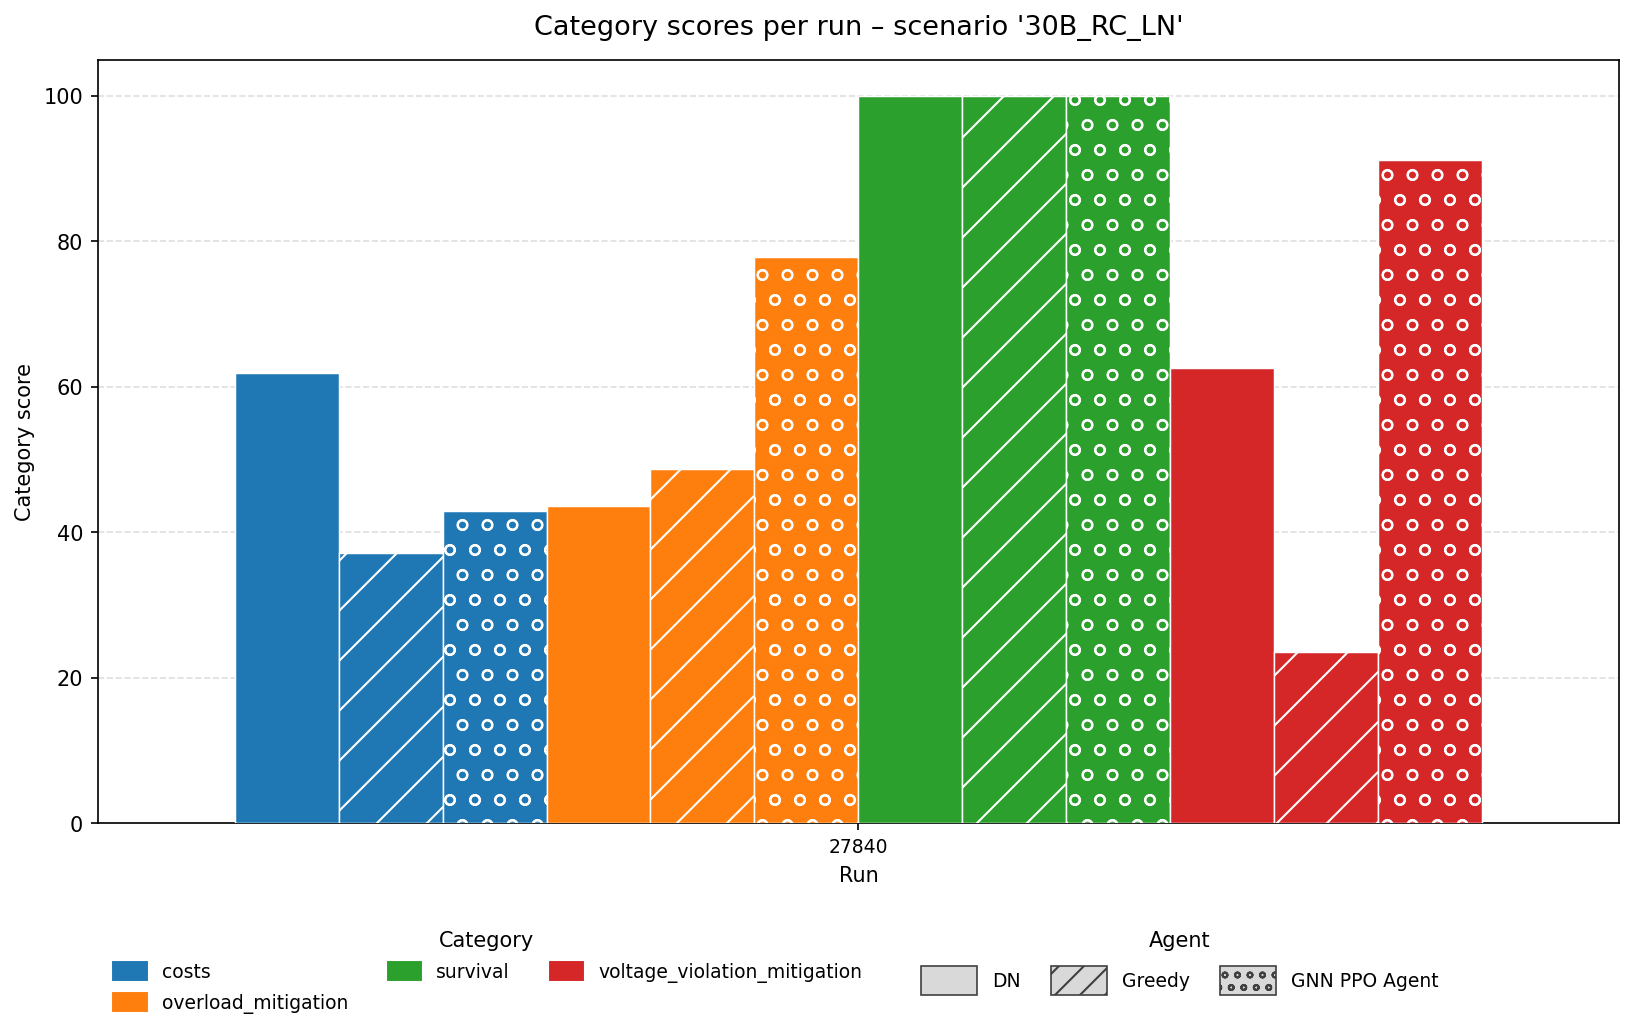
\includegraphics[width=0.7\textwidth]{images/experiments/scenario_scores/30B_RC_LN.png}
    \caption{Score overview over the scenario in the 30-bus power grid with lowered line capacity}
    \label{fig:scenario-scores-rc} 
\end{figure}

\FloatBarrier



\subsection{Stress Test Scenarios}
Figures \ref{fig:scenario-scores-gn-stress} to \ref{fig:scenario-scores-rc-stress} show the category scores achieved by the three agents on the individual scenarios composing the stress test experiments introduced in Section \ref{sec:exp-stress-test}, covering the lowest and highest stress levels of generator scaling, load scaling, and line capacity reduction. The second level of stress is already shown in the previous section.

\begin{figure}[htp] % htp = hier (h), top (t), oder auf einer eigenen Seite (p).
    \centering
    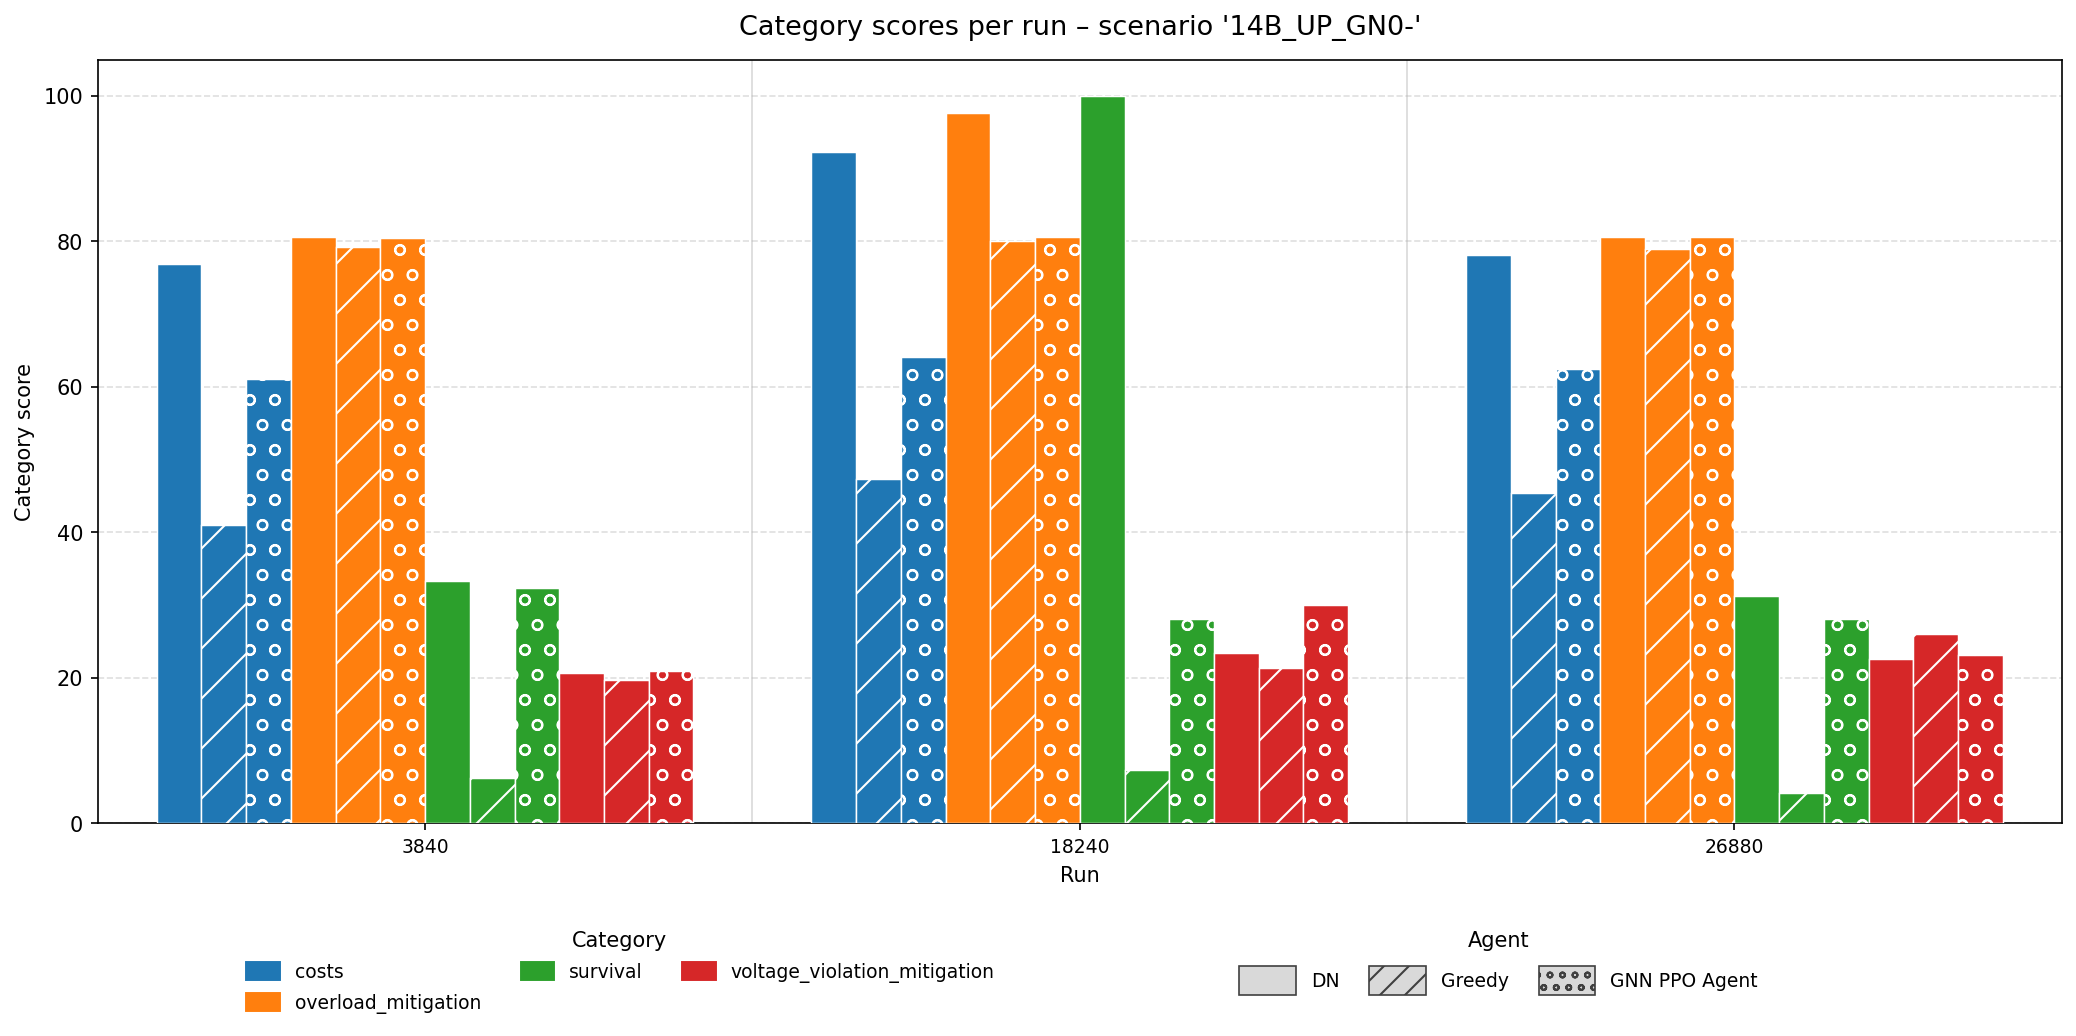
\includegraphics[width=0.95\textwidth]{images/experiments/scenario_scores/14B_UP_GN0-.png}
    \caption{Score overview over the scenario in the 14-bus power grid with lowest level of increased power generation in generator 0}
    \label{fig:scenario-scores-gn-stress} 
\end{figure}

\begin{figure}[htp]
    \centering

    \begin{subfigure}[t]{0.95\textwidth}
        \centering
        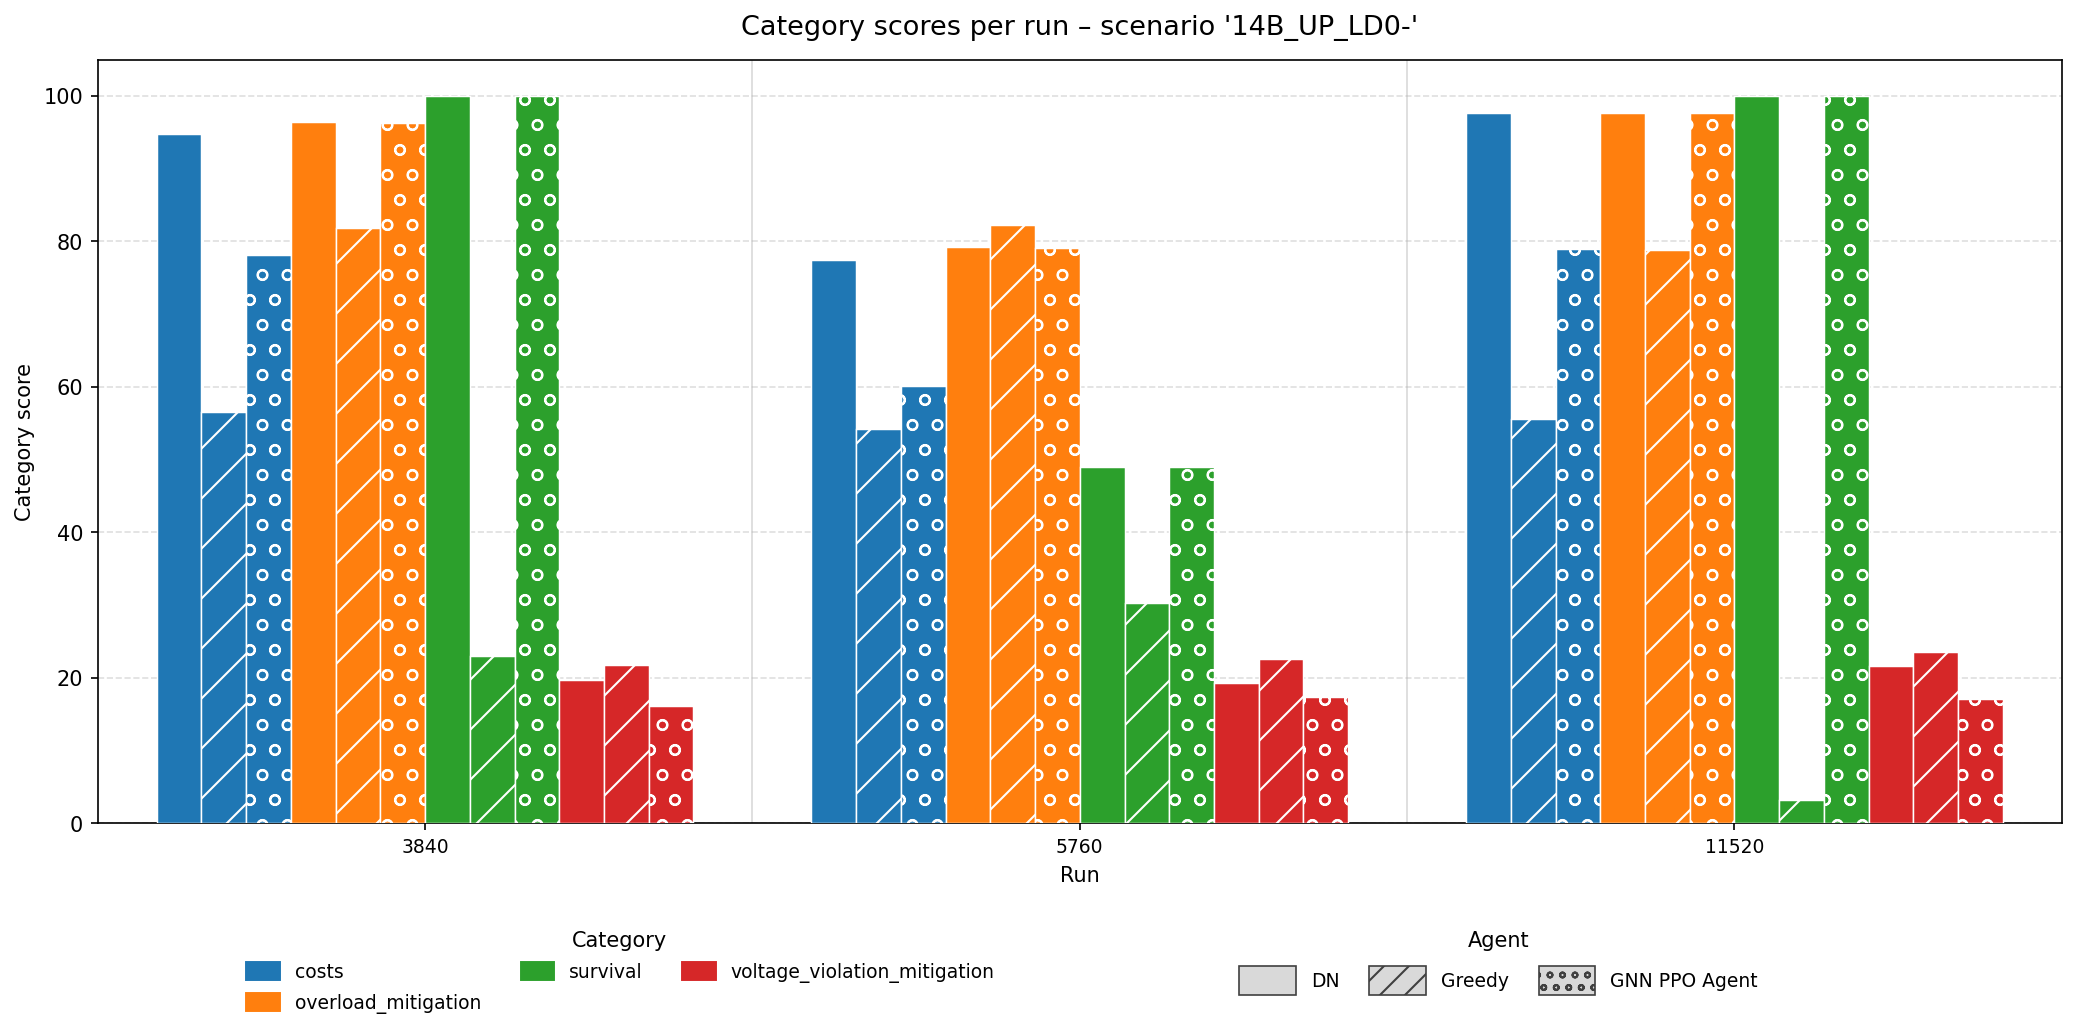
\includegraphics[width=\textwidth]{images/experiments/scenario_scores/14B_UP_LD0-.png}
        \caption{14-bus with lowest increased power consumption in load 0}
        \label{fig:scenario-scores-14b-up-ld0-low}
    \end{subfigure}

    \vspace{0.2em}

    \begin{subfigure}[t]{0.65\textwidth}
        \centering
        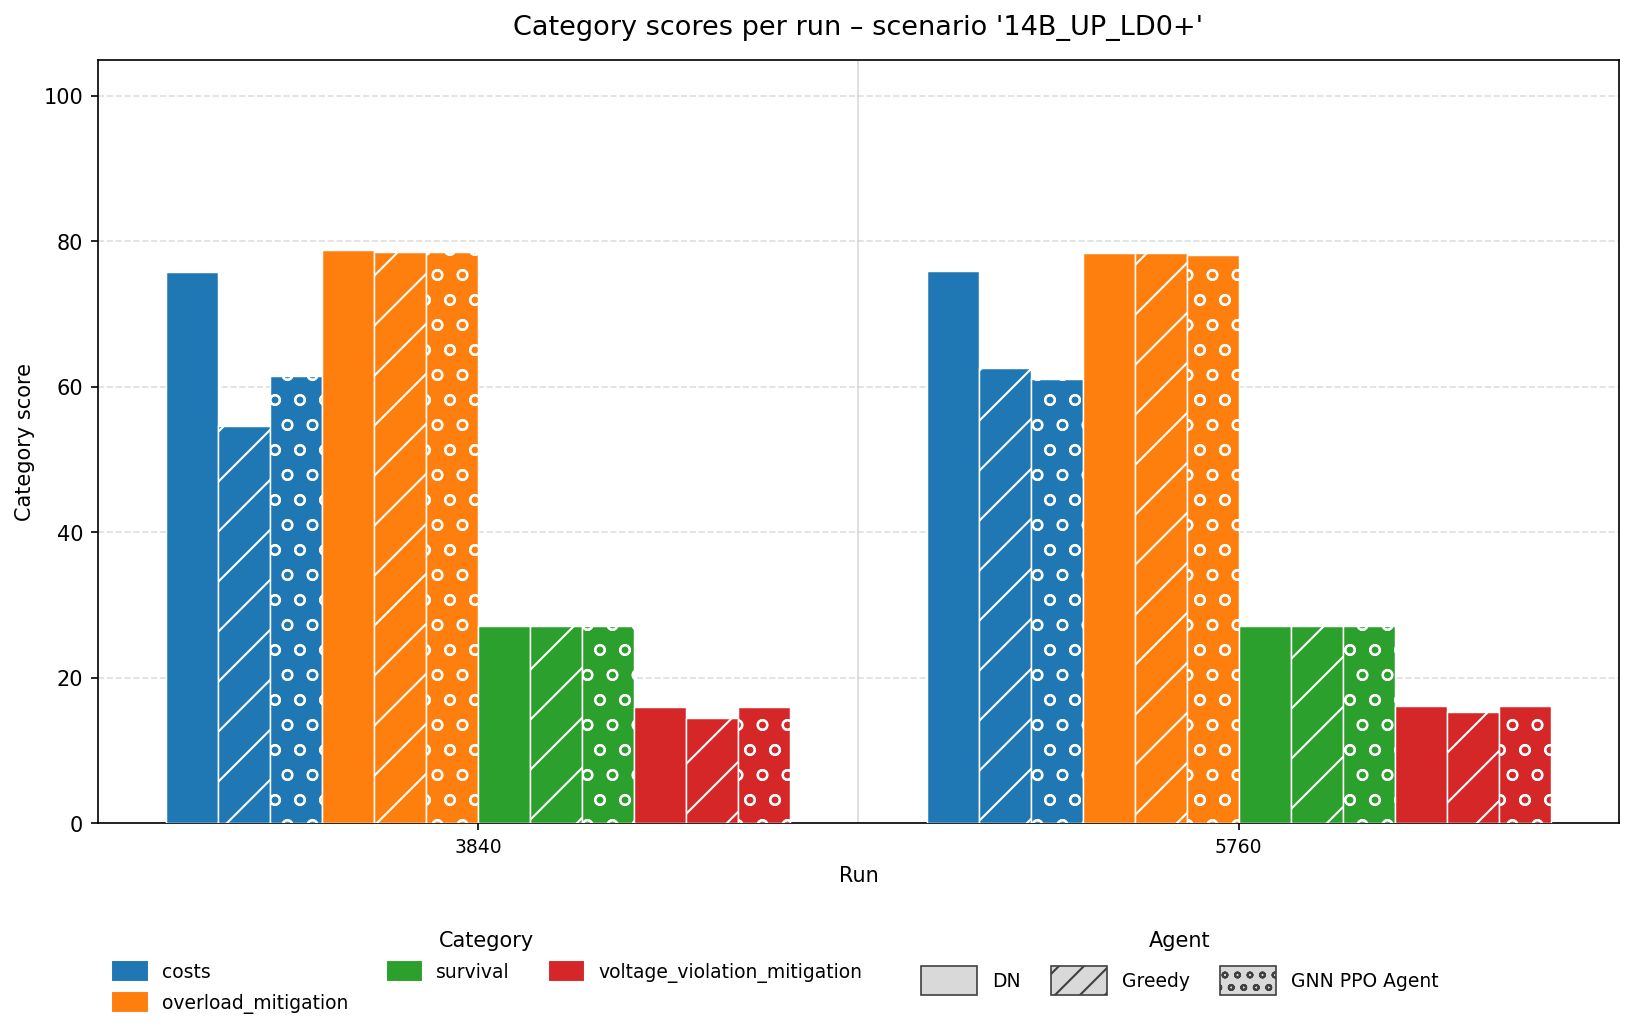
\includegraphics[width=\textwidth]{images/experiments/scenario_scores/14B_UP_LD0+.png}
        \caption{14-bus with highest increased power consumption in load 0}
        \label{fig:scenario-scores-14b-up-ld0-high}
    \end{subfigure}

    \caption{Score overview over the stress test scenario with different levels of load consumption scaling}
    \label{fig:scenario-scores-ld-stress}
\end{figure}

\begin{figure}[htp]
    \centering

    \begin{subfigure}[t]{0.65\textwidth}
        \centering
        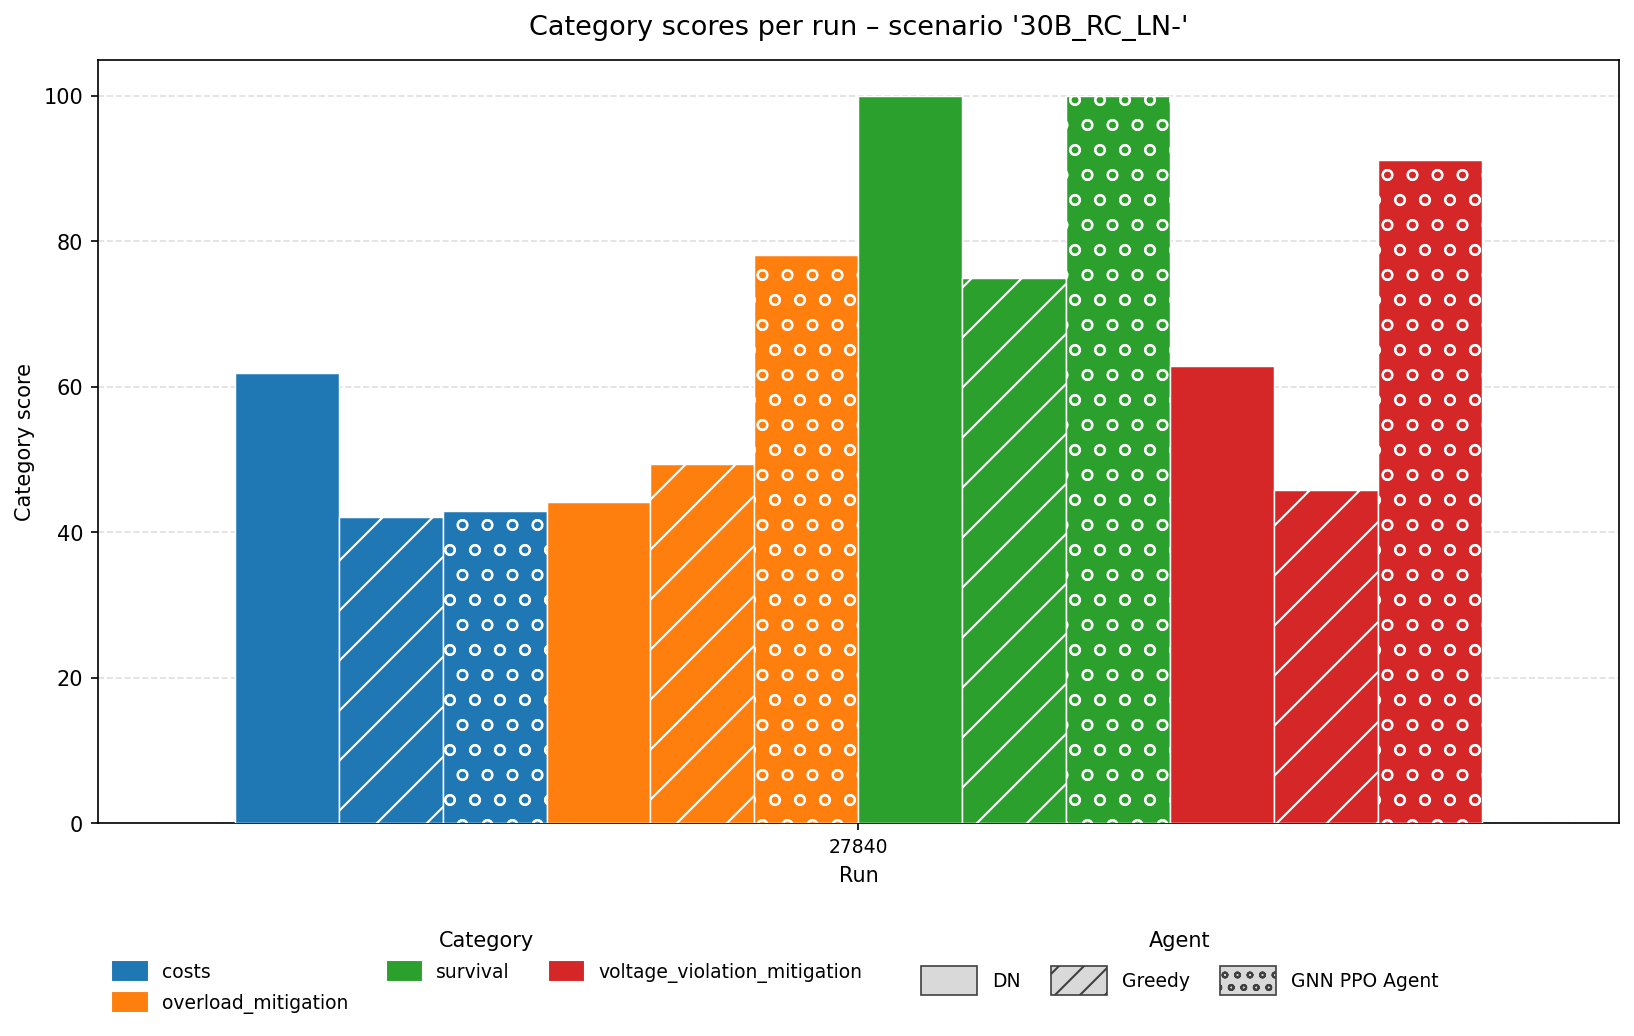
\includegraphics[width=\textwidth]{images/experiments/scenario_scores/30B_RC_LN-.png}
        \caption{30-bus with lowest reduced line capacity}
        \label{fig:scenario-scores-30b-rc-ln-low}
    \end{subfigure}

    \vspace{0.2em}

    \begin{subfigure}[t]{0.65\textwidth}
        \centering
        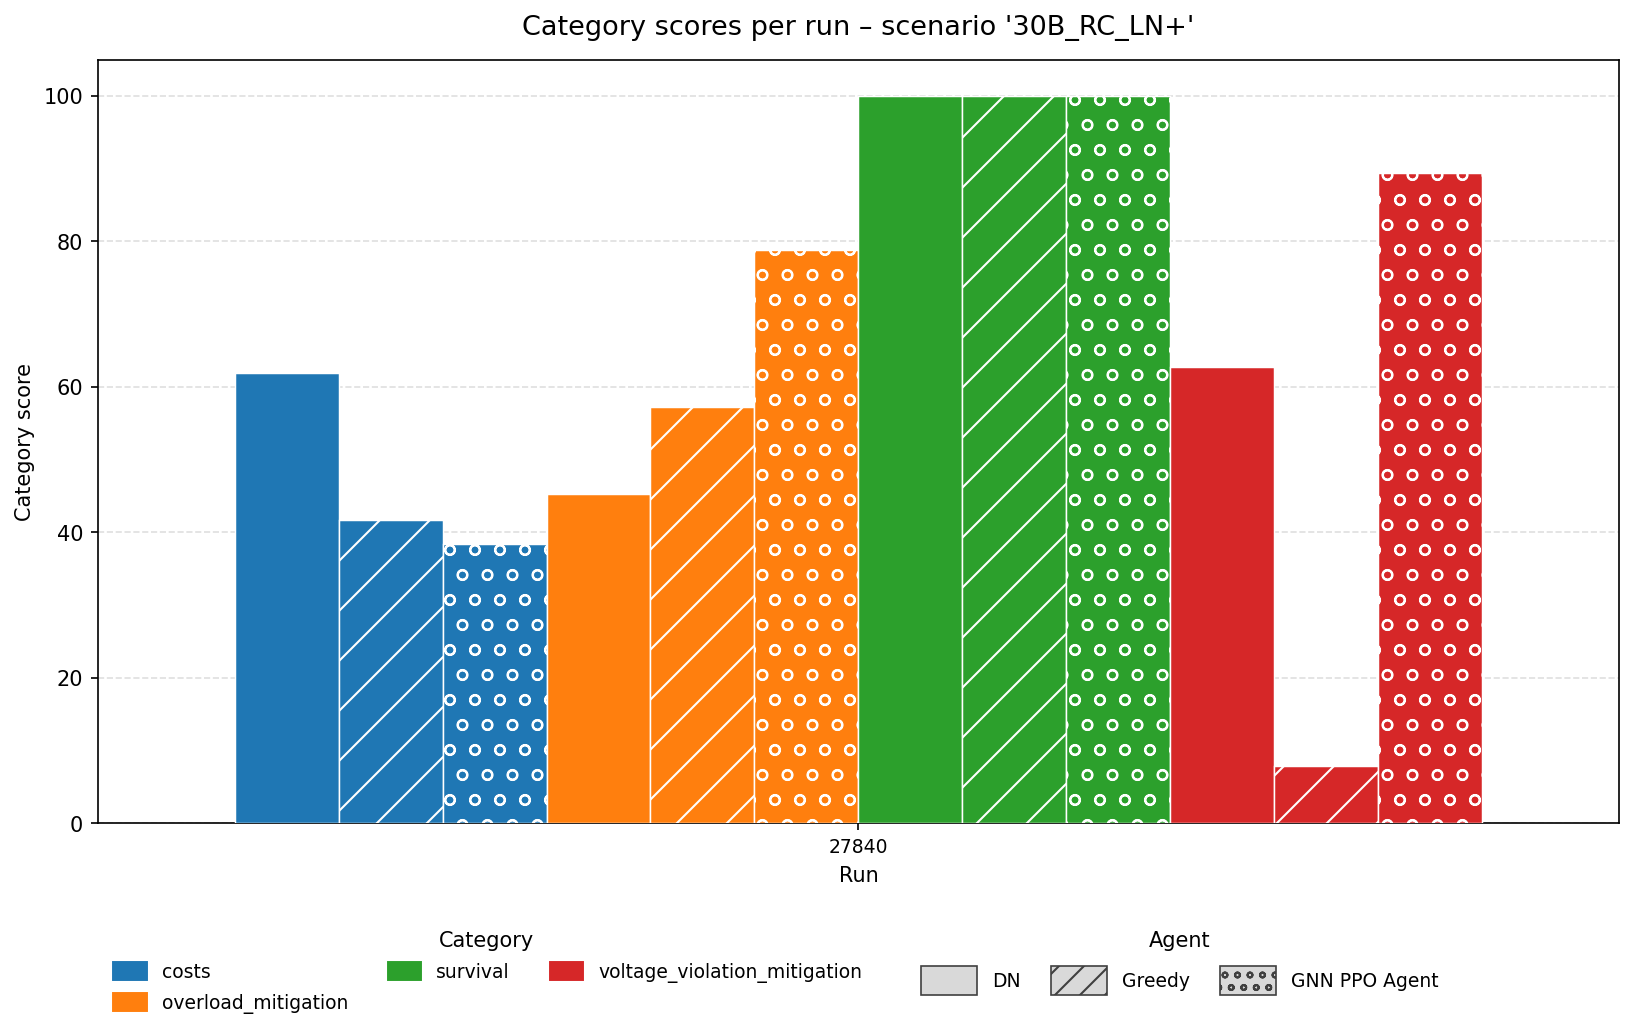
\includegraphics[width=\textwidth]{images/experiments/scenario_scores/30B_RC_LN+.png}
        \caption{30-bus with highest reduced line capacity}
        \label{fig:scenario-scores-30b-rc-ln-high}
    \end{subfigure}

    \caption{Score overview over the stress test scenario with different levels of line capacity scaling}
    \label{fig:scenario-scores-rc-stress}
\end{figure}

\FloatBarrier


\section{Case Study}\label{sec:exp-case-study}
Figure \ref{fig:grids-case-study} illustrates the partial grid topologies which result from the \ac{ppo} agent's substation-splitting actions in the three case studies discussed in Section \ref{ssec:case-studies}.

\begin{figure}[htp]
    \centering
    \begin{subfigure}[b]{0.48\textwidth}
        \centering
        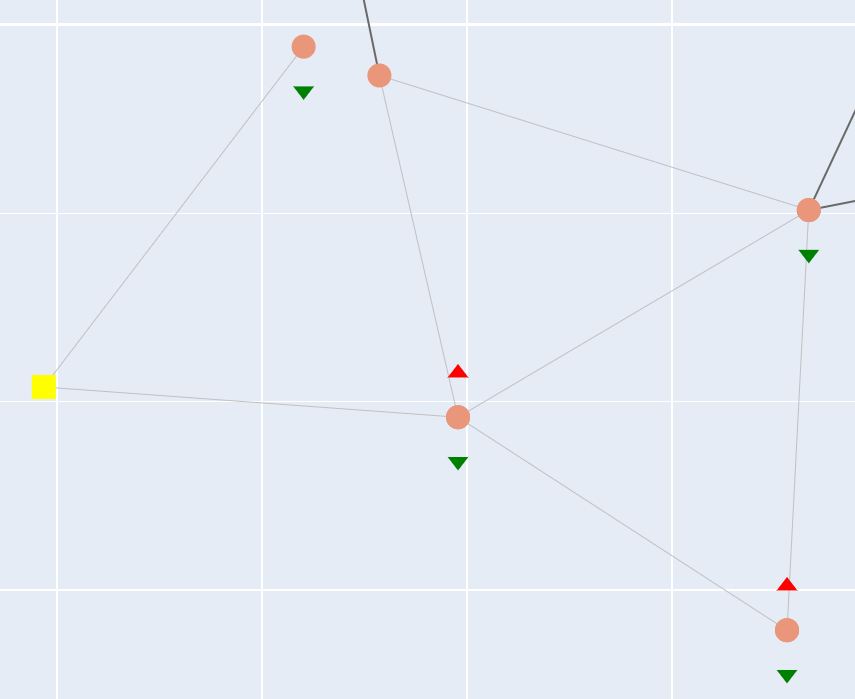
\includegraphics[width=\textwidth]{images/experiments/grids/case_study1.png}
        \caption{Partial power grid of case study 1, after the \ac{ppo} splitting action}
        \label{fig:grid-case-study1}
    \end{subfigure}
    \hfill
    \begin{subfigure}[b]{0.49\textwidth}
        \centering
        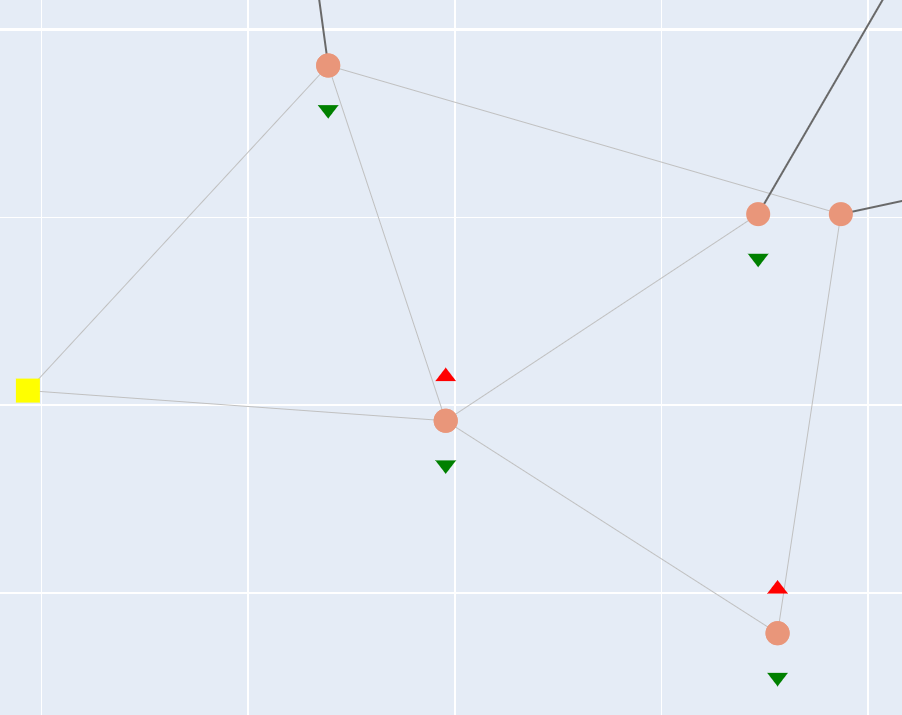
\includegraphics[width=\textwidth]{images/experiments/grids/case_study2.png}
        \caption{Partial power grid of case study 2, after the \ac{ppo} splitting action}
        \label{fig:grid-case-study2}
    \end{subfigure}

    \vspace{1em}

    \begin{subfigure}[b]{0.49\textwidth}
        \centering
        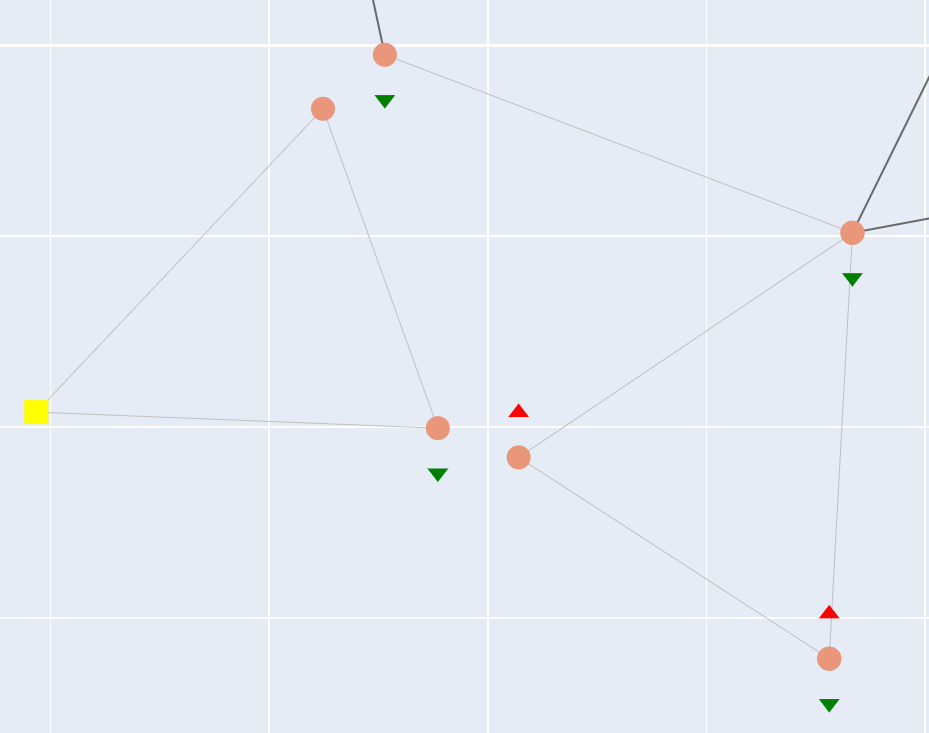
\includegraphics[width=\textwidth]{images/experiments/grids/case_study3.png}
        \caption{Partial power grid of case study 3, after the \ac{ppo} splitting actions}
        \label{fig:grid-case-study3}
    \end{subfigure}
    \caption{Power grids showing the actions made of the \ac{ppo} agent for the three case studies}
    \label{fig:grids-case-study}
\end{figure}

\FloatBarrier
\end{document}
